\documentclass[12pt, oneside, a4paper]{enetcom-pfe-report}

\graphicspath{{images/}}

%% TODO: Remove this function when done %%
%\newcommand\todoin[2][]{\todo[inline, caption={2do}, #1]{
%\begin{minipage}{\textwidth-4pt}#2\end{minipage}}}

%%%%%%%%%%%%%%%%%%%%%%%%%%%%%%%%%%%%%%%%%%%%%%%%%%%%%%%%%%%
% Include useful commands
%%%%%%%%%%%%%%%%%%%%%%%%%%%%%%%%%%%%%%%%%%%%%%%%%%%%%%%%%%%
\newcommand{\reportTitle}{Taha Mortadha PFE}
\newcommand{\reportSubject}{PFE}
\newcommand{\reportAuthor} {%
  Taha Omrani Mortadha  \textsc{Boufaid}%
}
\renewcommand{\tablename}{Tableau}
\hypersetup{
  pdftitle={\reportTitle~-~\reportSubject},%
  pdfauthor={\reportAuthor},%
  pdfsubject={\reportSubject},%
  pdfkeywords={report} {internship} {pfe} {Iset}
}
\dominitoc

\begin{document}

    \doublespacing{}% Double spacing between lines
    \pagenumbering{roman}% i ii iii iv ...
    
    \chapter*{DEDICACE}
%\addstarredchapter{DEDICATION}
%\addcontentsline{toc}{chapter}{DEDICATION}
%\adjustmtc
\thispagestyle{MyStyle}
\begin{center}

 {\huge \textbf{Nous dédions ce livre}}

 \vspace{0.5cm}\textbf{A Nos Parents.}

Aucun mot ne peut suffire à exprimer l’amour et la reconnaissance que nous vous porte.
Merci pour tous les efforts et les sacrifices que vous avez inlassablement
consentis pour notre éducation et notre bien-être. J’espère que vous serez toujours fiers de nous. nous vous honore à travers ce modeste travail, en témoignage de notre reconnaissance éternelle et de notre amour infini.\par


\textbf{À Nos très chers amis}

Qui ont animé ces années et ont rendu toutes les épreuves plus agréables, apportant ainsi des couleurs à notre vie. À ceux qui nous ont connu et qui ont contribué, de près ou de loin, à notre réussite.

\begin{minipage}{0.7\textwidth}
\hfill\large\textbf{Taha Omrani  Mortadha Boufaid}
\end{minipage}
\end{center}


    \chapter*{REMERCIEMENTS}
%\addstarredchapter{REMERCIEMENTS}
%\addcontentsline{toc}{chapter}{REMERCIEMENTS}
%\adjustmtc
\thispagestyle{MyStyle}
\begin{sloppypar}
\begin{center}

C’est avec un grand plaisir que nous réservons ces quelques lignes en signe de gratitude et de profonde reconnaissance à tous ceux qui, de près ou de loin, ont contribué à l’aboutissement de ce travail.\

Nous tenons à exprimer nos sincères remerciements au président du jury, \textbf{M. Boubaker Atef}, pour sa présence et sa participation active lors de la soutenance de notre rapport de fin d'étude. Sa présence en tant que président du jury a été un honneur, et nous sommes reconnaissants de son expertise et de ses conseils tout au long de ce processus d'évaluation.

Nous tenons également à remercier notre rapporteur, \textbf{M. Sami Hadhri}, pour son expertise, ses critiques constructives et ses suggestions pertinentes qui ont grandement amélioré la qualité de notre travail.

Nous remercions très vivement \textbf{Mme Ben Salah Manel} pour la confiance qu’elle nous a accordée pour réaliser notre projet de fin d’études, son encadrement, son assistance et son suivi incessant par ses directives et ses conseils précieux.

Nous tenons à remercier notre encadrant de l’entreprise, \textbf{M. Ahmed Nasser}, pour sa disponibilité, ses critiques constructives, son encouragement et ses conseils judicieux.

Nous exprimons notre profonde gratitude et notre reconnaissance au corps professoral de \textbf{l'Institut Supérieur des Études Technologiques de Sfax} pour la qualité de la formation qu'ils nous ont donnée. En effet, nous avons commencé notre première expérience professionnelle avec des bases solides grâce à leurs apports et leurs conseils.

Nos remerciements s’adressent également à tous les membres de l’équipe \textbf{développement} de la société \textbf{InfoObject Software}.

\end{center}
\end{sloppypar}
   
    \addtocontents{toc}{\protect\thispagestyle{MyStyle}}
    \renewcommand*\contentsname{TABLE DES MATIÈRES}
    \begin{spacing}{1}
    \tableofcontents
    \end{spacing}

    \addtocontents{lof}{\protect\thispagestyle{MyStyle}}
    \renewcommand{\listfigurename}{LISTE DES FIGURES}
    \begin{spacing}{1}
    \listoffigures
    \end{spacing}
  
    
    \addtocontents{toc}{\protect\thispagestyle{MyStyle}}
    \renewcommand*\contentsname{LISTE DES TABLEAUX}
    \begin{spacing}{1}
    \listoftables
    \end{spacing}

    
    \cleardoublepage
    \pagenumbering{arabic}% 1 2 3 4 5
    \setcounter{page}{1}
    
    \doublespacing{}% Double spacing between lines
    %\addtocontents{toc}{\protect\setcounter{tocdepth}{2}}
    
    % Réglage du compteur de chapitre pour le chapitre 11
    % \setcounter{chapter}{11}
        
    \chapter*{INTRODUCTION GÉNÉRALE}
\markboth{\MakeUppercase{INTRODUCTION GÉNÉRALE}}{}
\addcontentsline{toc}{chapter}{INTRODUCTION GÉNÉRALE}
\adjustmtc
\thispagestyle{MyStyle}
\begin{sloppypar} 
\vspace{-13mm}
Avec la croissance exponentielle du marché des applications mobiles, le développement d’applications dédiées à divers besoins est crucial. Dans le domaine de l’éducation, notamment pour les étudiants universitaires, l’accès à des informations pertinentes et la gestion efficace des services posent des défis significatifs.

\vspace{-1mm}
Actuellement, les étudiants font face à plusieurs défis majeurs pour gérer leur vie universitaire, notamment la difficulté à trouver des logements près de l'université et à accéder aux installations comme les bibliothèques et les cafés, souvent dispersées sur différentes plateformes. De plus, la recherche d'informations essentielles comme les événements, les stages, et les calendriers d'examens est complexe, nécessitant la consultation de multiples systèmes et applications.

\vspace{-1mm}
Notre solution consiste à développer une plateforme centralisée qui rassemble toutes ces données sous un même toit, permettant aux étudiants d'accéder facilement et rapidement à des informations fiables sur les logements disponibles et les facilités. En centralisant ces informations, nous visons à simplifier et optimiser significativement l'expérience des étudiants dans la gestion de leurs activités académiques et personnelles.

\vspace{-1mm}
Ce rapport détaille neuf chapitres : \textbf{Le premier} présente l’organisme d’accueil et le projet, avec étude de l’existant et solution proposée. \textbf{Le deuxième} traite de l'architecture logicielle, des outils utilisés et de la méthodologie de gestion de projet. \textbf{Le troisième} couvre les stratégies de test et le processus de déploiement. \textbf{Le quatrième} aborde la gestion des utilisateurs. \textbf{Le cinquième} explore la gestion des universités, des lieux et des examens. \textbf{Le sixième} examine la gestion des transports, des événements et des stages. \textbf{Le septième} traite des publications et des notifications. \textbf{Le huitième} explore les cartes, les conversations en ligne et les tableaux de bord. Une conclusion évalue le travail accompli et les futures perspectives.

\vspace{-1mm}
En conclusion, nous présenterons une synthèse de notre travail ainsi que les perspectives d'extension de ce projet.
\end{sloppypar}
\endinput
 
    \chapter{Chapitre 1: Etude préalable}
\begin{spacing}{1.2}
\minitoc
\thispagestyle{MyStyle}
\end{spacing}
\newpage
\renewcommand{\tablename}{Tableau}
\begin{sloppypar} 

\section{Introduction }
\vspace{-4mm}
Ce chapitre vise à situer le projet dans son contexte général. Nous débutons en présentant l'entreprise d'accueil, InfoBjectif. Ensuite, nous identifions la problématique et définissons le contexte global pour positionner le projet dans son environnement organisationnel, méthodologique et stratégique. Nous terminons en critiquant l'état actuel des choses, en présentant la solution proposée et la méthodologie à suivre, ainsi que la gestion du temps pour les différentes tâches du projet sous la forme d'un diagramme de Gantt. 
\vspace{-6mm}
\section{Organisme d’accueil  }
\vspace{-4mm}
InfoBjectif est une entreprise de Services en Ingénierie Informatique (SSII) . Nous débutons cette section en présentant InfoBjectif, et concluons en exposant l'organigramme de l'équipe au sein de laquelle j’ai effectué mon stage de fin d'études .
\vspace{-6mm}
\subsection{Présentation de Infobjectif}
\vspace{-4mm}
\subsubsection{Introduction}
\vspace{-4mm}
Infobjectif se positionne comme un acteur majeur dans le domaine de la transformation numérique sur le marché tunisien. L'entreprise offre une gamme complète de services, incluant le conseil, l'intégration de systèmes, le déploiement de solutions métiers, la gestion d'infrastructure et des services de processus d'entreprise. Cette diversité de services permet aux grandes entreprises de relever les défis liés au développement et à la compétitivité dans un environnement numérique en constante évolution.

\begin{figure}[H]%
    \center%
    \setlength{\fboxsep}{5pt}%
    \setlength{\fboxrule}{0.5pt}%
    \fbox{
    
\includegraphics[width=5cm]{images/InfoLogo.png}%
    }
    \caption{Logo Infobjectif}%
\end{figure}

\subsubsection{Coordonnées de l'entreprise}

\begin{flushleft}
\textbf{Adresse:} Tunis, Rue Nijer \\
\textbf{Téléphone:} 23236236 \\
\textbf{Adresse e-mail:} infoobjectif@gmail.com
\end{flushleft}

\subsection{Organigramme de la societé}
\vspace{-4mm}
la figure 1.2 présente l'organigramme de la societé : 
\begin{figure}[H]%
    \center%
    \setlength{\fboxsep}{5pt}%
    \setlength{\fboxrule}{0.5pt}%
    \fbox{
    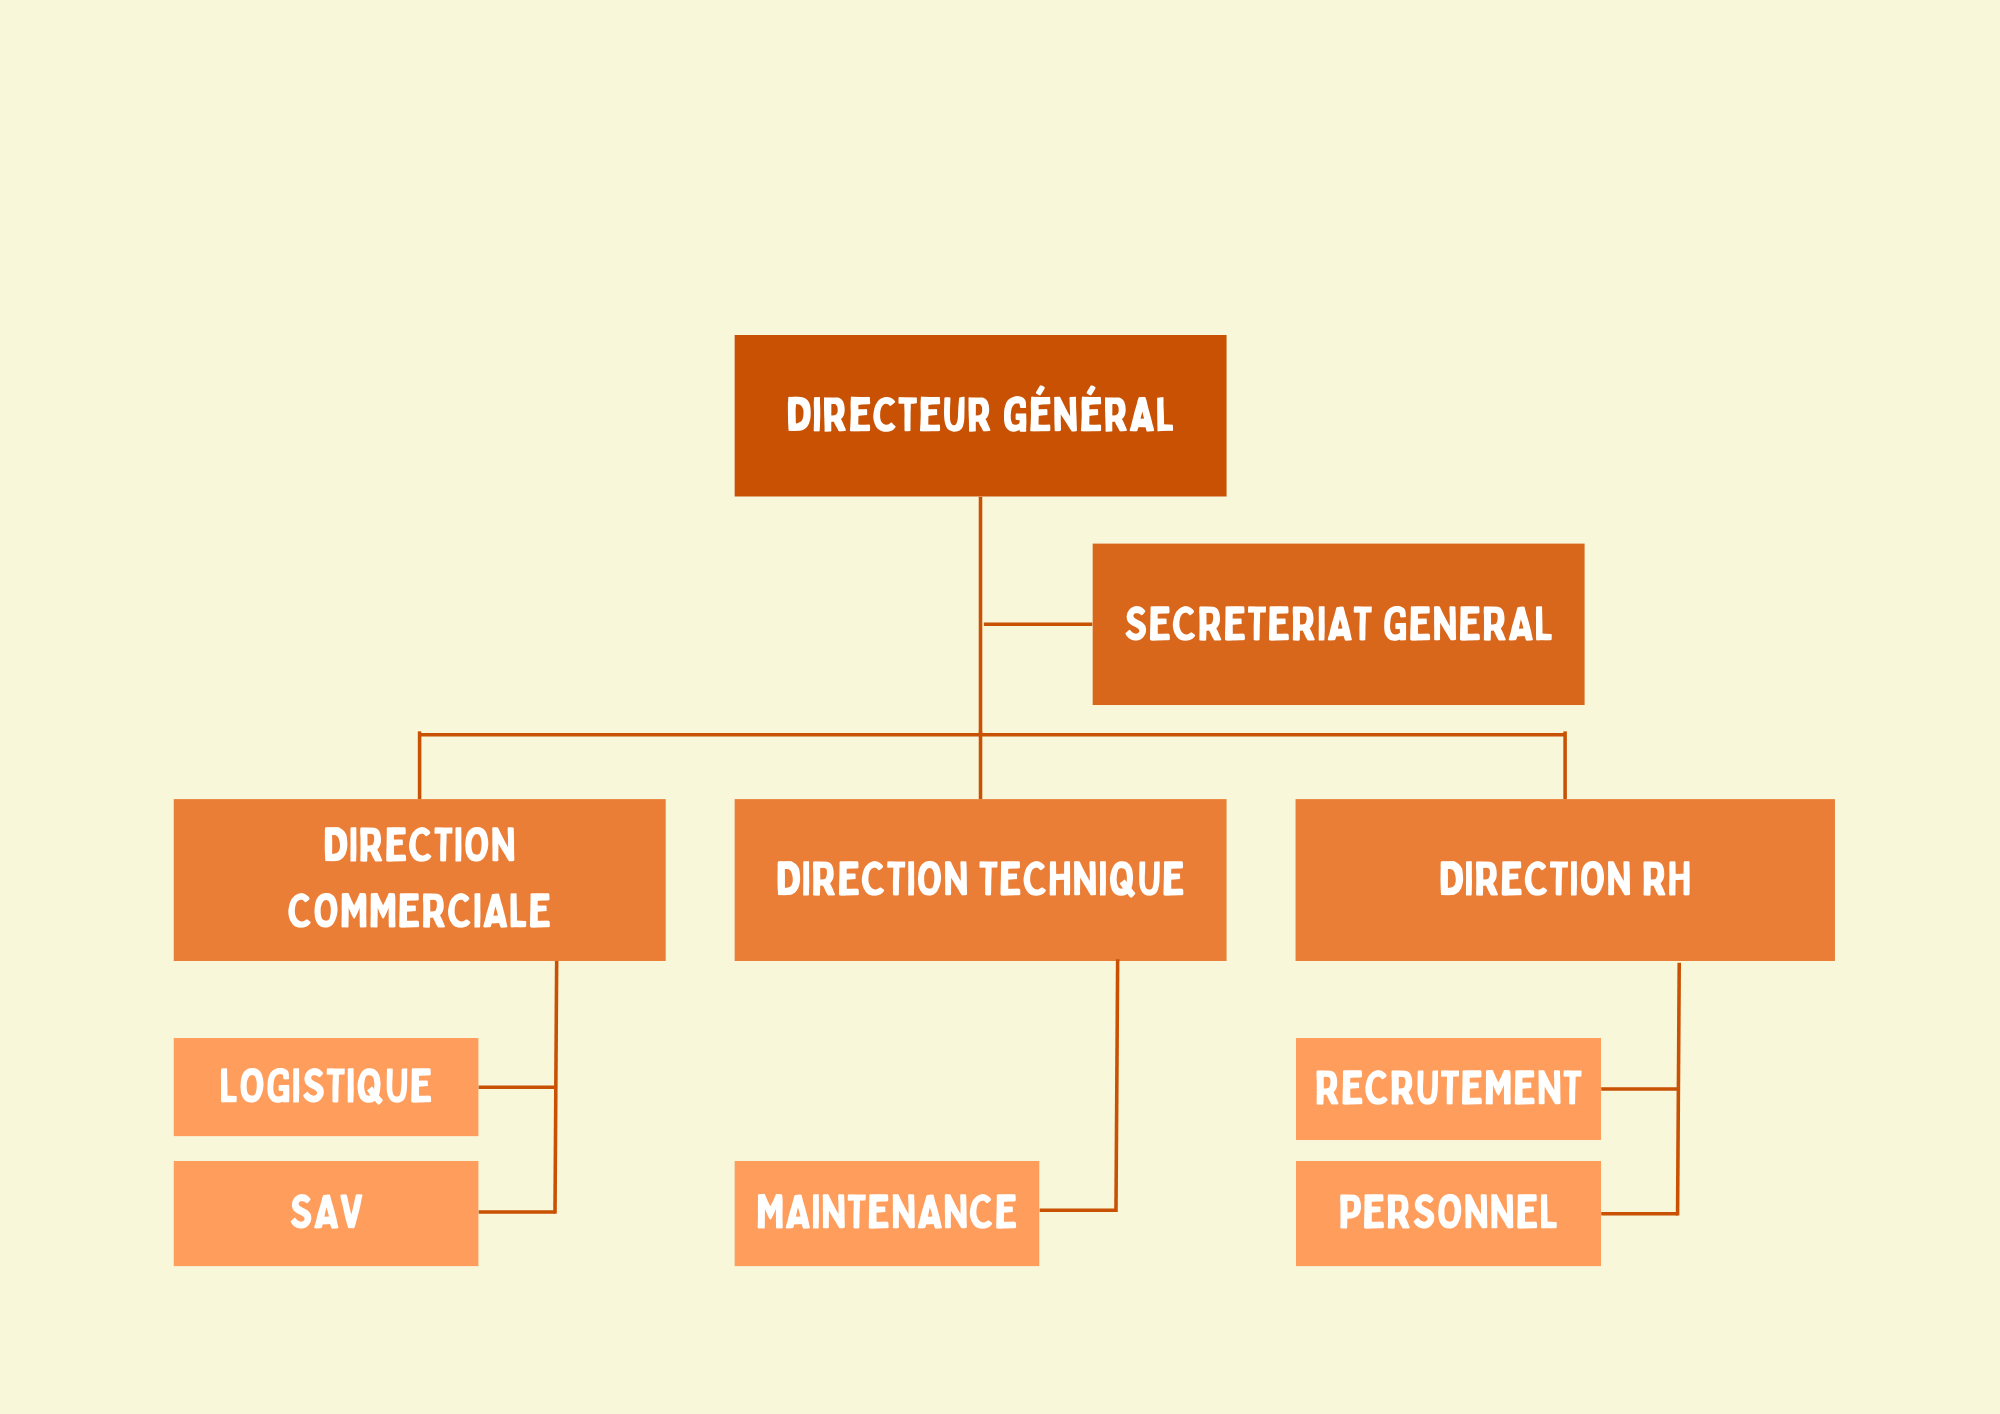
\includegraphics[width=15cm]{images/Organigramme infobjectif.png}%
    }
    \caption{Organigramme de L'entreprise}%
\end{figure}
\vspace{-15mm}
\section{Présentation du projet}
\vspace{-6mm}
\subsection{Contexte du projet}
\vspace{-4mm}
Nous avons pour mission dans le cadre de notre projet de fin d'études en vue de l’obtention de la Licence Appliquée en Technologie de L’Informatique DSI.
Il consiste à la conception et le développement d’une application web et mobile  de gestion
des services pour les etudians et de communication 
une période de 14 semaines.

\vspace{-9mm}
\subsection{Etude de l’existant }
\vspace{-4mm}
L'étude de l'existant met en évidence les différents systèmes et pratiques actuels utilisés par les étudiants pour accéder aux informations universitaires et communiquer avec l'administration. Actuellement, les informations importantes, telles que les événements sur le campus et les offres de stage, sont disponibles sur divers supports, y compris les sites web, les panneaux d'affichage et les réseaux sociaux. Chaque support contient des informations spécifiques, nécessitant souvent des recherches sur plusieurs plateformes pour obtenir une vue d'ensemble complète. De plus, il y a une dispersion des informations sans centralisation claire, ce qui peut augmenter le temps nécessaire pour trouver des informations précises. Les outils actuels manquent de fonctionnalités avancées de filtrage et de personnalisation, ce qui rend la recherche d'informations spécifiques plus complexe. Ces observations montrent l'opportunité de développer une solution numérique centralisée pour améliorer l'accès aux informations et la communication au sein de l'université.
\vspace{-6mm}
\subsection{Critique de l’existant }
\vspace{-4mm}
La fragmentation de l'information est un problème clé, avec des données cruciales dispersées sur divers supports tels que les sites web, les panneaux d’affichage et les réseaux sociaux, compliquant ainsi l'accès rapide et efficace aux informations nécessaires. Cette dispersion entraîne également un manque de centralisation, obligeant les étudiants à rechercher les mêmes informations sur plusieurs plateformes, ce qui conduit à une perte de temps considérable. De plus, les canaux de communication existants sont inefficaces et ne répondent pas adéquatement aux besoins des étudiants, rendant difficile l'interaction rapide et efficace avec l'administration universitaire. Enfin, l'absence de fonctionnalités de filtrage et de personnalisation complique encore davantage la recherche d’informations, empêchant les étudiants de trouver facilement les informations les plus pertinentes pour eux.
\vspace{-6mm}
\section{Solution proposée}
\vspace{-4mm}
\adjustmtc
\thispagestyle{MyStyle}
\vspace{-4mm}
Pour répondre aux défis rencontrés par les étudiants dans leur recherche d’informations pertinentes et leur communication avec l’administration universitaire, nous proposons la mise en place d’une solution numérique centralisée et efficace. Cette solution permettra de regrouper toutes les données dispersées sur différents supports tels que les sites web, les panneaux d’affichage et les réseaux sociaux. En centralisant ces informations, nous offrirons aux étudiants un accès simplifié et rapide à toutes les données dont ils ont besoin. De plus, notre solution comprendra des fonctionnalités avancées de filtrage et de personnalisation, permettant à chaque utilisateur de trouver facilement les informations pertinentes tout en réduisant considérablement le temps nécessaire à leur recherche.

Pour résoudre ces problèmes, notre solution centralise à :
\begin{itemize}
    \item Rassembler toutes les informations dispersées sur divers supports au sein d'une plateforme numérique unique pour un accès unifié et fiable.
    \item Intégrer des options avancées de filtrage permettant aux étudiants de sélectionner et d'afficher uniquement les informations pertinentes selon leurs besoins spécifiques.
    \item Intégrer des outils de communication efficaces comme des messageries instantanées pour faciliter les échanges entre étudiants et administration, améliorant ainsi la résolution rapide des problèmes et la réponse aux questions en temps réel.
\end{itemize}

Cette approche vise à optimiser l'expérience des étudiants en leur fournissant un accès facile et structuré aux informations essentielles, tout en améliorant l'efficacité globale de la communication au sein de l'université.

\vspace{-6mm}
\section{Méthodologie du travail }
\vspace{-4mm}
La méthodologie du travail pour la réalisation de cette solution numérique, peut être décomposée en plusieurs étapes clés :

\underline{\textbf{Analyse des besoins : }} Comprendre en profondeur les besoins des étudiants et des administrateurs universitaires en termes d'informations, de communication et d'interactions. Cela implique des entretiens avec les parties prenantes, des sondages et des études de marché pour identifier les fonctionnalités et les exigences essentielles de la plateforme.

\underline{\textbf{Conception de l'architecture :}} Concevoir une architecture logicielle robuste qui prend en charge les fonctionnalités souhaitées tout en garantissant la scalabilité, la performance et la sécurité. Cette étape comprend également la définition des interfaces utilisateur et des flux de navigation pour une expérience utilisateur optimale.

\underline{\textbf{Développement frontend : }} Développement d'une application mobile destinée aux étudiants, et la conception d'une interface d'administration web. L'accent sera mis sur la création d'interfaces utilisateur intuitives et faciles à utiliser, avec une navigation fluide et des fonctionnalités accessibles, pour assurer une expérience utilisateur optimale.

\underline{\textbf{Développement backend : }}Implémentation du backend de l'application pour gérer efficacement les requêtes des utilisateurs et assurer la gestion optimale des données. Cette phase inclut la création de services pour répondre aux besoins fonctionnels de l'application et la mise en place d'une infrastructure de base de données pour le stockage sécurisé des informations essentielles.


\underline{\textbf{Intégration continue et déploiement : }} Mettre en place des pipelines d'intégration continue pour automatiser les tests et les déploiements, assurant ainsi la qualité du code et la stabilité de l'application tout au long du processus de développement. Utiliser des outils tels que Jenkins, GitLab CI ou GitHub Actions pour cette tâche.

\vspace{-6mm}
 \subsection{UP (Processus Unifié) }
 \vspace{-4mm}
 Le processus unifié est une méthode d’implémentation et de développement, majoritairement utilisée par les développeurs informatiques. Il s’agit d’un processus itératif et implémentable. Il est caractérisé par quatre aspects : 
\\1.	Un pilotage par les cas d’utilisation 
\\2.	L’architecture au cœur du processus
\\3.	L’utilisation maximale des modèles, plus spécifiquement des modèles UML 
\\4.	La levée régulière des incertitudes grâce à sa dimension itérative et cyclique [1].
\vspace{-6mm}
\subsection{SCRUM : Agile}
\vspace{-4mm}
La méthode SCRUM définit un cadre de travail permettant la réalisation de projets complexes. Initialement prévu pour le développement de projets type « Software », cette méthode peut être appliquée à tout type de projet, du plus simple au plus innovant, et ce de manière très simple. Cette méthodologie permet de s’adapter rapidement aux changements du client à fréquence régulière. Chaque fin d'itération, l'équipe et le client réévaluent les spécifications du logiciel [2].
\vspace{-6mm}
\subsection{Comparaison des méthodes }
\vspace{-4mm}
Pour remédier aux problèmes de la complexité de gestion des projets de développement informatique, le génie logiciel a proposé des démarches avec étapes bien précises dont le but est d’avoir un système conforme aux normes et aux standards de développement. Le tableau ci-dessous décrit une étude comparative entre les méthodes les plus courantes :
\begin{table}[h]
\centering
\setlength{\extrarowheight}{4pt}
\caption{Comparison between SCRUM and UP}
\begin{tabularx}{\textwidth}{|>{\raggedright\arraybackslash}X|>{\raggedright\arraybackslash}X|>{\raggedright\arraybackslash}X|}
\hline 
\multicolumn{3}{|c|}{\textbf{Méthodes}} \\
\hline
\textbf{} & \textbf{SCRUM} & \textbf{UP} \\
\hline
\textbf{Développement incrémental} & Durée d'un sprint (1 à 4 semaines) & Fin d'une itération "construction" \\
\hline
\textbf{Développement itératif} & 1 mois MAX & Dépend de la taille du projet \\
\hline
\textbf{Justification économique} & Planification avec la "valeur métier" pour seul critère de priorité & Document de "vision" \\
\hline
\textbf{Degré d'interaction} & Haut : client impliqué, réunions de scrum quotidiennes, réunions de sprint & Moyen \\
\hline
\textbf{Principales différences} & Aucune préconisation technique (Souvent couplé à XP), auto-organisation & Formalisme plus important, approche pilotée par les risques centrée sur l'architecture, conduit par les cas d'utilisation proches de la cascade \\
\hline
\end{tabularx}
\end{table}
\vspace{-6mm}
\subsection{Choix de la méthodologie adoptée }
\vspace{-4mm}
Nous nous sommes intéressées à la méthode Scrum. \\
\vspace{-1mm}
$\surd$\underline{ \textbf{  Pourquoi Scrum ?}}
       Sa force est de se reposer sur des cycles de développements courts, adaptés en permanence, sans jamais perdre de vue l’expérience utilisateur (UX). \\
\vspace{-1mm}
\underline{ \textbf{Parmi ses bénéfices }} 
\renewcommand{\labelitemi}{\tiny$\bullet$}
\begin{itemize}[leftmargin=1cm, topsep=0pt]
\vspace{-1mm}
 \item  Une gestion plus souple, plus intelligente du travail, améliorant l’efficacité des équipes. 
\vspace{-1mm}
 \item Une meilleure visibilité du projet et de son évolution.  
\vspace{-1mm}
 \item Une communication interne renforcée, et donc une meilleure cohésion d’équipe.   
\vspace{-1mm}
 \item Le partage des savoirs et la favorisation de l’entraide.  
\vspace{-1mm}
 \item Un gain de temps et une meilleure réactivité grâce aux réunions fréquentes et aux insights du client.
\end{itemize}
\vspace{-1mm}
\underline{ \textbf{Les intervenants dans Scrum }}\\
\vspace{-1mm}
        La méthode Scrum regroupe trois acteurs : le Product Owner, le Scrum Master et l’équipe de développement. Dans cette partie, nous allons voir plus en détail le rôle de chacun de ces acteurs. 
\renewcommand{\labelitemi}{\tiny$\bullet$}
\begin{itemize}[leftmargin=1cm, topsep=0pt]
\vspace{-2mm}
\item \textbf{Le Product Owner }: il est considéré comme le chef de projet et est responsable de la vision du produit à réaliser. Il est chargé de définir les spécifications fonctionnelles en créant et en gérant le backlog produit, qui recueille les besoins du client.
\vspace{-1mm}
\item \textbf{Le Scrum Team} : il s'agit des membres de l'équipe de développement qui sont responsables de la réalisation des tâches selon leur ordre de priorité, ainsi que de la livraison du produit final.
\vspace{-1mm}
\item\textbf{ Sprint }:
Un Sprint est une itération, il s’agit d’une période généralement entre 2 et 4 semaines maximum pendant laquelle une version terminée et utilisable du produit est réalisée. Un nouveau Sprint commence dès la fin du précédent. Chaque Sprint a un objectif et une liste de fonctionnalités à réaliser [5].
\end{itemize}
\vspace{-8mm}
\subsection{Glossaire SCRUM }
\vspace{-6mm}
la figure suivante présente un schéma illustratif de la méthodologie SCRUM [3].

\vspace{-2mm}
\begin{figure}[H]%
    \center%
    \setlength{\fboxsep}{5pt}%
    \setlength{\fboxrule}{0.5pt}%
    \fbox{
    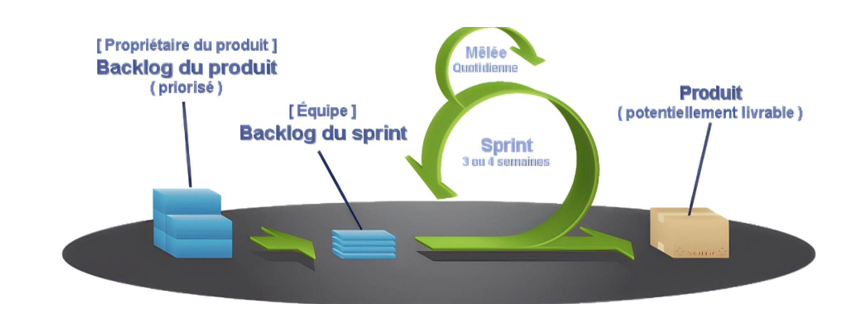
\includegraphics[width=14cm,height=6cm]{images/scrum.png}%
    }
\caption{Schéma illustratif de la méthodologie SCRUM}
\end{figure}
\vspace{-6mm}
\subsection{Justification du choix de SCRUM }
\vspace{-4mm}
Le recours à cette méthodologie est justifié uniquement lorsque SCRUM est utilisé pour garantir un produit de haute qualité, tout en respectant certains principes immuables tels que :\\
-	Tolérer tous les changements, même tardifs, apportés au cours du développement.\\
-	Livrer une application fonctionnelle.\\
-	Créer un projet autour de personnes motivées en leur fournissant un environnement et un soutien, et en leur faisant confiance.\\
-	Garantir un rythme de travail efficace.\\
-	Permettre aux membres de l'équipe de s'auto-organiser et de rechercher la simplicité.

\vspace{-7mm}

\section{Conclusion }
\vspace{-4mm}
Dans ce chapitre, nous avons introduit le cadre de notre stage en présentant l'entreprise d'accueil et en identifiant la problématique, suivie de la proposition d'une solution. Ensuite, nous avons exposé la méthode SCRUM que nous avons choisi d'adopter pour la réalisation de notre projet. Dans le chapitre suivant, nous allons procéder à l'analyse de l'outil \textbf{JIRA}.
    


\end{sloppypar}


 
    \chapter{ Chapitre 2: Architecture 
\centering logicielle et outils de travail}
\begin{spacing}{1.2}
\minitoc
\thispagestyle{MyStyle}
\end{spacing}
\newpage
\begin{sloppypar} 

\section{Introduction}
\vspace{-3mm}
Dans le chapitre précédent, nous avons abordé l’étude du projet. Dans ce nouveau chapitre, nous allons commencer par dresser la liste des acteurs qui interagissent avec le système. Ensuite, nous définirons les besoins fonctionnels et non fonctionnels de notre solution. En nous appuyant sur cette analyse, nous élaborerons une spécification détaillée de la solution choisie en utilisant des diagrammes de cas d’utilisation. Ce sprint est consacré à comprendre l’architecture logicielle et à mettre en œuvre cette dernière à travers les frameworks de développement.
\vspace{-9mm}
\section{Capture des besoins}
\vspace{-4mm}
\subsection{Définition des acteurs }
\vspace{-3mm}
Un acteur représente l’abstraction d’un rôle joué par des entités externes quiinteragissent
directement avec le système étudié. Notre application va contenir deux acteurs :

\begin{itemize}
    \item[$\bullet$] Admin : Le superviseur possède tous les droits d'accès aux paramètres de l'application web et mobile.
    \item[$\bullet$] Étudiant : Habituellement, il a accès à son compte. Il a la capacité de consulter, d'afficher, de modifier son profil et de créer des publications.
\end{itemize}
\vspace{-9mm}

\subsection{Besoins fonctionnels }
\vspace{-3mm}
Les besoins fonctionnels seront traduits par les services offerts par notre futur système.
Ils identifient les tâches ou les activités qui doivent être formulées par l’application pour les différents types d’acteurs. Pour notre futur système, les fonctionnalités sont très riches. Nous
proposons de les classer selon les acteurs responsables comme suit :
\begin{itemize}
\item [•] \textbf{Le Admin} doit être capable de :

→ S’authentifier : Saisir un login et un mot de passe pour accéder à son espace.\\
→ Gérer le profil :L'admin peut modifier ses informations personnelles.\\
→ Consulter la liste des utilisateurs de l’application.\\
→ Consulter la liste des Endroits de l’application.\\
→ Consulter la liste des evenements de l’application.\\
→ Consulter la liste des universites de l’application.\\
→ Consulter la liste des stages de l’application.\\
→ Consulter la liste des moyens de transport de l’application.\\
→ Communiquer avec les utlisateurs  de l’application.\\
→ Créer une publication sur  l’application.\\
→ Commenter sur  une publication dans  l’application.

\item [•] \textbf{L'etudiant } doit être capable de :

→ S’inscrire : L'etudiant doit créer un compte pour pouvoir accéder à l’application mobile.\\
→ S’authentifier :Saisir un login et un mot de passe pour accéder à son espace.\\
→ Gérer le profil :L'etudiant peut modifier ses informations personnelles.\\
→ communiquer avec l'admin de l’application.\\
→ créer une publication sur  l’application.\\
→ commenter sur  une publication dans  l’application.
\end{itemize}
\vspace{-5mm}
\subsection{Besoins non-fonctionnels}
\vspace{-3mm}
Les besoins non fonctionnels représentent les contraintes internes et externes à vérifier pour le futur système. Parmi les besoins non fonctionnels de notre futur système, nous pouvons citer :

\begin{itemize}
    \item Besoins d’utilisation : le système doit fournir des interfaces ergonomiques, claires et simples à utiliser.
    \item La performance : L’application à développer doit être principalement performante, c’est-à-dire, à travers ses fonctionnalités, elle doit répondre correctement à toutes les exigences des usagers.
    \item Besoins de sécurité : Le système doit interdire l’accès de tout intrus par les droits et les privilèges d’accès.
    \item L’extensibilité : La caractéristique open source de l’application va permettre son extensibilité en rajoutant de nouvelles fonctionnalités ou en modifiant des fonctionnalités déjà développées.
\end{itemize}

\vspace{-2cm}


\section{Backlog de produit  }
\vspace{-7mm}
Le backlog du produit est le cœur de Scrum. C’est ici que tout commence. Un backlog du produit est essentiellement une liste hiérarchisée d’exigences, d’histoires, de fonctionnalités ou d'autres contenus. Il représente ce que le client souhaite, décrit en termes de client. Le tableau suivant décrit le « Backlog du produit » et présente les « Histoires utilisateurs ».

\vspace{19mm}

\vspace{-2cm}
\begin{longtable}{|p{1.5cm}|p{11cm}|p{2cm}|}
\hline
\textbf{Priorité} & \textbf{Histoire Utilisateur} & \textbf{Complexité} \\
\hline
\endfirsthead
\hline
Priorité & Histoire Utilisateur & Complexité \\
\hline
\endhead
1 & En tant qu’un étudiant, je peux créer un compte dans l’application mobile. & Moyenne \\
\hline
2 & En tant qu’un utilisateur, je peux réinitialiser mon mot de passe sur la partie mobile. & Simple \\
\hline
3 & En tant qu’un utilisateur (administrateur et étudiant), je peux m’authentifier dans l’application mobile. & Moyenne \\
\hline
4 & En tant qu’un administrateur, je peux m’authentifier à l’application web. & Moyenne \\
\hline
5 & En tant qu’un administrateur, je peux supprimer les étudiants depuis l’application web. & Simple \\
\hline
6 & En tant qu’un utilisateur, je peux modifier les données de mon compte. & Difficile \\
\hline
7 & En tant qu’un étudiant, je peux gérer mon compte. & Difficile \\
\hline
8 & En tant qu’un administrateur, je peux gérer les universités dans l’application web. & Moyenne \\
\hline
9 & En tant qu’un administrateur, je peux gérer les événements dans l’application web. & Moyenne \\
\hline
10 & En tant qu’un administrateur, je peux gérer les facilités dans l’application web. & Moyenne \\
\hline
11 & En tant qu’un administrateur, je peux gérer les offres de stages dans l’application web. & Moyenne \\
\hline
12 & En tant qu’un administrateur, je peux gérer les stations de transports dans l’application web. & Moyenne \\
\hline
13 & En tant qu’un administrateur, je peux gérer les examens dans l’application web. & Moyenne \\
\hline
14 & En tant qu’un utilisateur, je peux consulter les examens sur l'application mobile. & Moyenne \\
\hline
15 & En tant qu’un étudiant, je peux consulter la carte avec filtrage des données. & Difficile \\
\hline
16 & En tant qu’un étudiant, je peux consulter les détails des facilités qui apparaissent dans la carte dans l’application mobile. & Moyenne \\
\hline
17 & En tant qu’un étudiant, je peux consulter la carte Map pour chercher les facilités et les moyens de transport. & Moyenne \\
\hline
18 & En tant qu’un étudiant, je peux consulter les localisations des événements et stages dans la carte. & Moyenne \\
\hline
19 & En tant qu’un étudiant, je peux consulter les publications de ma page d’accueil dans l’application mobile. & Moyenne \\
\hline
20 & En tant qu’un étudiant, je peux consulter mes publications de ma page profil dans l’application mobile. & Simple \\
\hline
21 & En tant qu’un étudiant, je peux commenter et réagir aux publications dans l’application mobile. & Difficile \\
\hline
22 & En tant qu’un étudiant, je peux supprimer mes publications dans l’application mobile. & Simple \\
\hline
23 & En tant qu’un administrateur, je peux créer des notifications personnalisées sur la partie web. & Simple \\
\hline
24 & En tant qu’un utilisateur, je peux consulter ma page profil sur la partie mobile. & Simple \\
\hline
25 & En tant qu’un étudiant, je peux contacter l’administrateur. & Simple \\
\hline
26 & En tant qu’un étudiant, je peux contacter l’administrateur sur l'application mobile. & Moyenne \\
\hline
27 & En tant qu’un administrateur, je peux consulter le tableau de bord dans l’application web. & Moyenne \\
\hline
\caption{Backlog de produit}
\end{longtable}

\vspace{-1.8cm}
\section{Découpage en sprint  }
\vspace{-5mm}
La planification de release en Scrum organise le travail en sprints pour une livraison incrémentale des fonctionnalités du produit, alignant ainsi les attentes des parties prenantes et assurant que le produit répond aux besoins du client à chaque itération. Le tableau ci-dessous détaille ce plan, incluant les "Histoires utilisateurs" pour chaque sprint ainsi que les dates de début et de fin prévues pour chaque période.\\
\\

\vspace{-2cm}
\small
\begin{center}
\begin{longtable}{|>{\raggedright}p{2.8cm}|>{\raggedright}p{8cm}|>{\raggedright\arraybackslash\small}p{1.9cm}|>{\raggedright\arraybackslash\small}p{1.8cm}|}

\hline
\textbf{Sprint} & \textbf{Tâches} & 
\textbf{Date Début} & \textbf{Date Fin} \\
\hline

\endfirsthead
\hline
Sprint & Tâches & Date Début & Date Fin \\
\hline
\endhead
Sprint 1: Gestion des Utilisateurs & 
\begin{itemize}
    \vspace{-0.8cm}
    \setlength{\leftskip}{-0.4cm}
    \item En tant qu’un étudiant, je peux créer un compte dans l’application mobile.
    \vspace{-0.2cm}
    \item En tant qu’un utilisateur, je peux réinitialiser mon mot de passe sur la partie mobile.
        \vspace{-0.2cm}
    \item En tant qu’un utilisateur (administrateur et étudiant), je peux m’authentifier dans l’application mobile.
        \vspace{-0.2cm}
    \item En tant qu’un administrateur, je peux m’authentifier à l’application web.
        \vspace{-0.2cm}
    \item En tant qu’un administrateur, je peux supprimer les étudiants depuis l’application web.
        \vspace{-0.2cm}
    \item En tant qu’un utilisateur, je peux modifier les données de mon compte.
        \vspace{-0.2cm}
    \item En tant qu’un étudiant, je peux gérer mon compte.
    
\end{itemize}
& 12/02/2024 & 06/03/2024 \\
\hline

Sprint 2: Gestion des Universités, Endroits et des Examens & 
\begin{itemize}
    \vspace{-0.8cm}
    \setlength{\leftskip}{-0.4cm}    
    \item En tant qu’un administrateur, je peux gérer les universités dans l’application web.
    \vspace{-0.2cm}
    \item En tant qu’un administrateur, je peux gérer les événements dans l’application web.
    \vspace{-0.2cm}
    \item En tant qu’un administrateur, je peux gérer les facilités dans l’application web.
    \vspace{-0.2cm}
    \item En tant qu’un administrateur, je peux gérer les offres de stages dans l’application web.
    \vspace{-0.2cm}
    \item En tant qu’un administrateur, je peux gérer les stations de transports dans l’application web.
    \vspace{-0.2cm}
    \item En tant qu’un administrateur, je peux gérer les examens dans l’application web.
\end{itemize}
& 07/03/2024 & 30/03/2024 \\
\hline

Sprint 3: Gestion des Transports, Evénements et des Stages & 
\begin{itemize}
    \vspace{-1cm}
    \setlength{\leftskip}{-0.4cm}
    \item En tant qu’un utilisateur, je peux consulter les examens sur l'application mobile.
    \vspace{-0.2cm}
    \item En tant qu’un étudiant, je peux consulter la carte avec filtrage des données.
    \item En tant qu’un étudiant, je peux consulter les détails des facilités qui apparaissent dans la carte dans l’application mobile.
    \vspace{-0.2cm}
    \item En tant qu’un étudiant, je peux consulter la carte Map pour chercher les facilités et les moyens de transport.
    \vspace{-0.2cm}
    \item En tant qu’un étudiant, je peux consulter les localisations des événements et stages dans la carte.
\end{itemize}
& 31/03/2024 & 23/04/2024 \\
\hline

Sprint 4: Gestion des Publications et des Notifications & 
\begin{itemize}
    \vspace{-0.8cm}
    \vspace{-0.2cm}
    \setlength{\leftskip}{-0.4cm}
    \item En tant qu’un étudiant, je peux consulter les publications de ma page d’accueil dans l’application mobile.
    \vspace{-0.2cm}
    \item En tant qu’un étudiant, je peux consulter mes publications de ma page profil dans l’application mobile.
    \vspace{-0.2cm}
    \item En tant qu’un étudiant, je peux commenter et réagir aux publications dans l’application mobile.
    \vspace{-0.2cm}
    \item En tant qu’un étudiant, je peux supprimer mes publications dans l’application mobile.
    \vspace{-0.2cm}
    \item En tant qu’un administrateur, je peux créer des notifications personnalisées sur la partie web.
    \vspace{-0.2cm}
    \item En tant qu’un utilisateur, je peux consulter ma page profil sur la partie mobile.
\end{itemize}
& 24/04/2024 & 15/05/2024 \\
\hline

Sprint 5: Recherche des données sur un Map, Gestion des tableaux de bord et des Messageries & 
\begin{itemize}
    \vspace{-0.8cm}
    \vspace{-0.2cm}
    \setlength{\leftskip}{-0.4cm}
    \item En tant qu’un étudiant, je peux contacter l’administrateur.
    \vspace{-0.2cm}
    \item En tant qu’un étudiant, je peux contacter l’administrateur sur l'application mobile.
    \vspace{-0.2cm}
    \item En tant qu’un administrateur, je peux consulter le tableau de bord dans l’application web.
\end{itemize}
& 16/05/2024 & 21/05/2024 \\
\hline

\caption{Tableau de planification de release (mis à jour avec dates)}
\end{longtable}
\end{center}

\vspace{10cm}

\section{Architecture du système  }
\vspace{-3mm}
Dans cette section, on commence par la présentation de l'architecture que nous avons choisie pour réaliser notre application. Bien évidemment, le choix de l’architecture adéquate dans la phase de conception de toute application est primordial, afin de garantir un fonctionnement correct, une meilleure performance et une maintenance facile.

\begin{figure}[H]%
    \center%
    \setlength{\fboxsep}{5pt}%
    \setlength{\fboxrule}{0.5pt}%
    \fbox{
    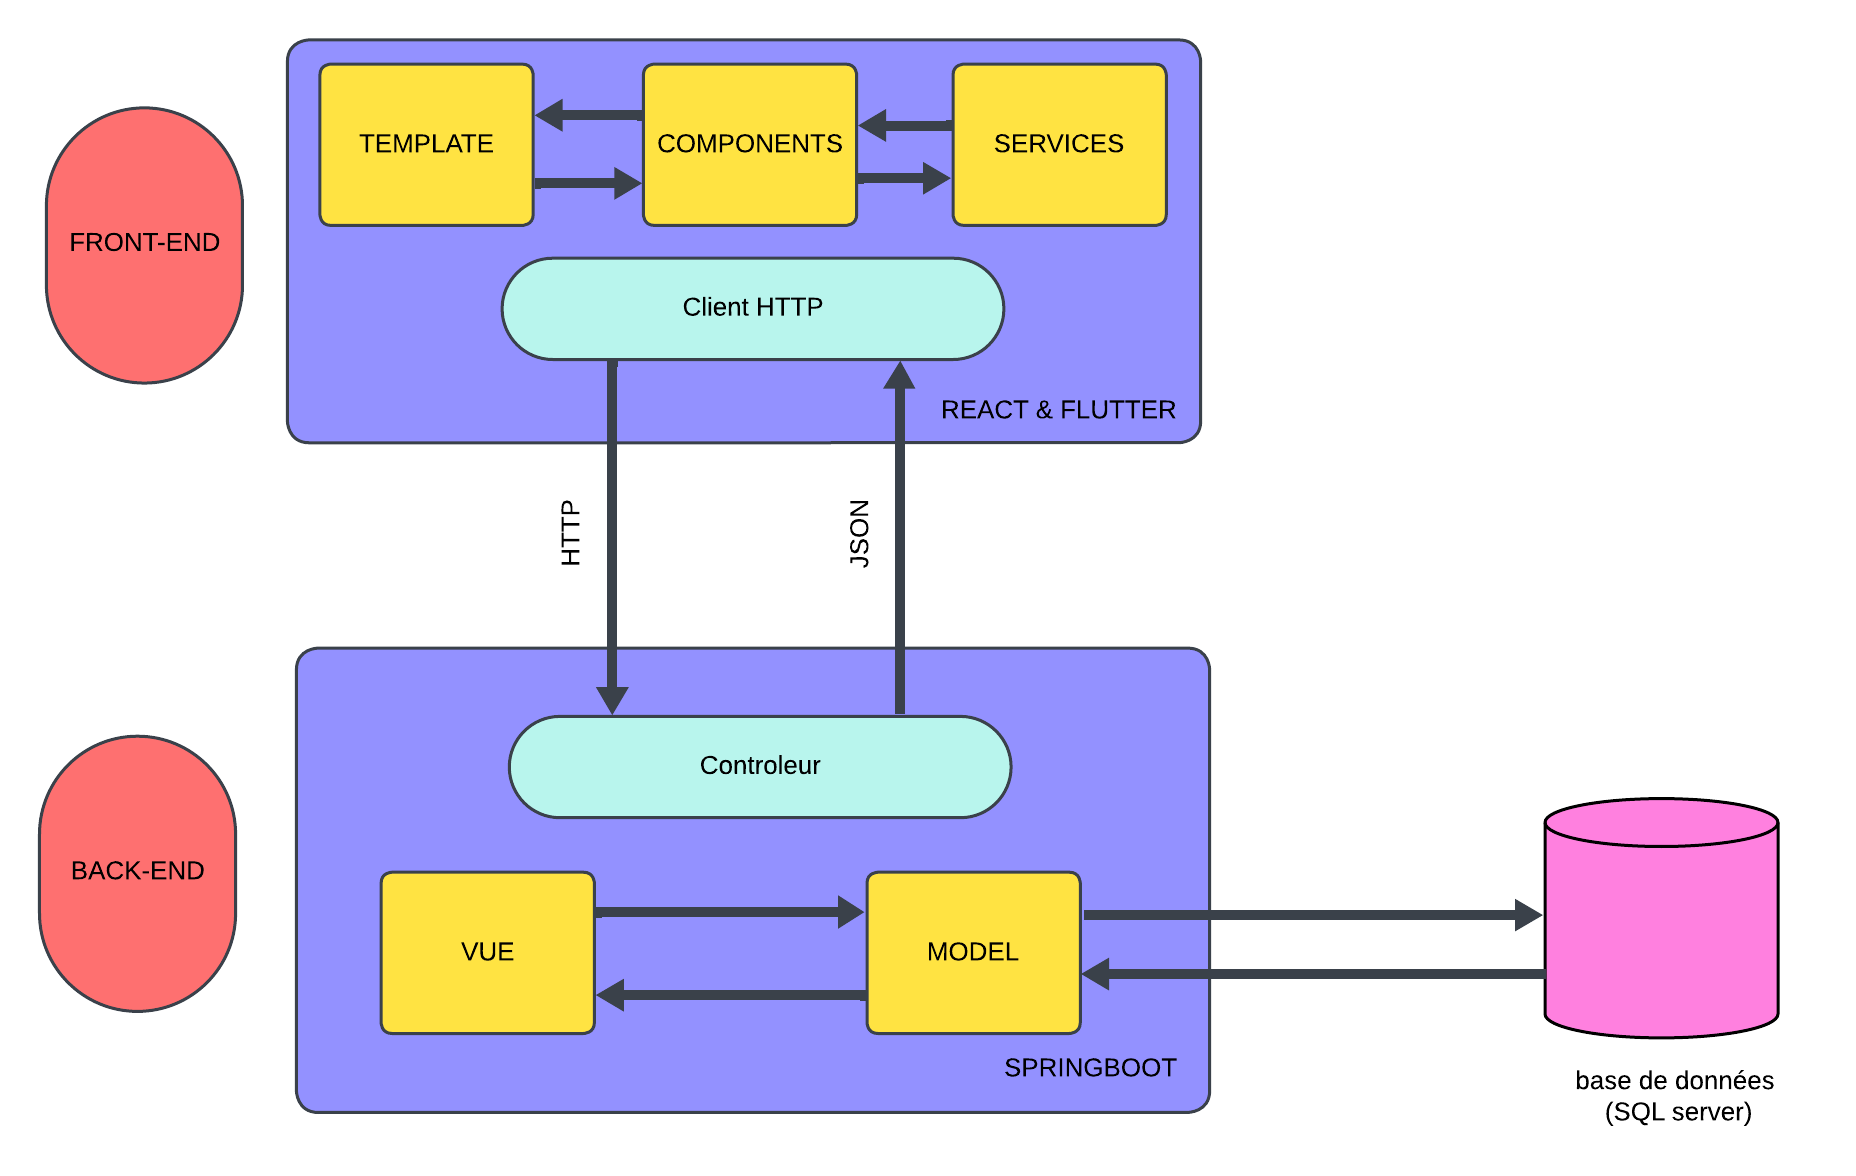
\includegraphics[height=12cm,width=15cm]{images/Brainstorming et idéation (2).png}%
    }
    \caption{Figure d'architecture du systéme}%
\end{figure}
\vspace{-1cm}
\section{Environnement de travail}

\vspace{-3mm}
Dans cette partie, nous nous intéressons d’abord à l’étude de l’environnement technique disponible pour la réalisation de mon projet. Ensuite, je justifie les choix pris en matière d’environnement logiciel pour mener à terme la partie applicative.
\vspace{-1cm}

% Partie Environnement logiciel
\section{Environnement logiciel}

\vspace{-4mm}

\subsection{Lucidchart}
\vspace{-3mm}
Lucidchart est une plateforme de collaboration en ligne, basée sur le cloud, permettant la création de diagrammes et la visualisation de données, et autres schémas conceptuels [4].
\begin{figure}[H]
    \centering
    \setlength{\fboxsep}{5pt}
    \setlength{\fboxrule}{0.5pt}
    \fbox{
\includegraphics[height=4cm,width=8cm]{images/lucidchart.png}}
    \caption{Logo Lucidchart}
\end{figure}
\vspace{-1.2cm}

\subsection{Figma}
\vspace{-3mm}
Figma est un éditeur de graphiques vectoriels et un outil de prototypage. Il est principalement basé sur le web, avec des fonctionnalités hors ligne supplémentaires activées par des applications de bureau pour macOS et Windows [5].
\begin{figure}[H]
    \centering
    \setlength{\fboxsep}{5pt}
    \setlength{\fboxrule}{0.5pt}
    \fbox{
\includegraphics[height=4cm,width=8cm]{images/figma.png}}
    \caption{Logo Figma}
\end{figure}
\vspace{-1.2cm}

% Partie Environnement de développement
\section{Environnement de développement}

\vspace{-3mm}

\subsection{Visual Studio Code}
\vspace{-3mm}
Visual Studio Code est un éditeur de code extensible développé par Microsoft pour Windows, Linux et macOS. Les fonctionnalités incluent la prise en charge du débogage, la mise en évidence de la syntaxe, la complétion intelligente du code, les snippets, la refactorisation du code et Git intégré [6]. 
\begin{figure}[H]
    \centering
    \setlength{\fboxsep}{5pt}
    \setlength{\fboxrule}{0.5pt}
    \fbox{
\includegraphics[height=4cm,width=8cm]{images/vscode.png}}
    \caption{Logo Visual Studio Code}
\end{figure}
\vspace{-1.5cm}

\subsection{IntelliJ IDEA}
\vspace{-4mm}
IntelliJ IDEA, également appelé « IntelliJ », « IDEA » ou « IDJ », est un environnement de développement destiné au développement de logiciels informatiques reposant sur la technologie Java [7]. 
\begin{figure}[H]
    \centering
    \setlength{\fboxsep}{5pt}
    \setlength{\fboxrule}{0.5pt}
    \fbox{
\includegraphics[height=4cm,width=8cm]{images/intellij.png}}
    \caption{Logo IntelliJ IDEA}
\end{figure}

\subsection{Android Studio}
\vspace{-4mm}
Android Studio est un environnement de développement pour développer des applications mobiles Android. Il est basé sur IntelliJ IDEA et utilise le moteur de production Gradle. Il peut être téléchargé sous les systèmes d'exploitation Windows, macOS, Chrome OS et Linux [8].
\begin{figure}[H]
    \centering
    \setlength{\fboxsep}{5pt}
    \setlength{\fboxrule}{0.5pt}
    \fbox{
\includegraphics[height=4cm,width=8cm]{images/androidstudio.png}}
    \caption{Logo Android Studio}
\end{figure}

% Autres outils pertinents
\subsection{Postman}
\vspace{-4mm}
Postman est une application permettant de tester des API, créée en 2012 par Abhinav Asthana, Ankit Sobti et Abhijit Kane à Bangalore pour répondre à une problématique de test d'API partageable [9].
\begin{figure}[H]
    \centering
    \setlength{\fboxsep}{5pt}
    \setlength{\fboxrule}{0.5pt}
    \fbox{
\includegraphics[height=4cm,width=8cm]{images/postman.png}}
    \caption{Logo Postman}
\end{figure}

\vspace{-2cm}
\section{Conclusion }
\vspace{-4mm}
Ce chapitre a présenté l'environnement de travail, les outils logiciels, les frameworks et les langages de programmation utilisés pour notre projet, facilitant une collaboration efficace. Nous avons défini les besoins fonctionnels et non fonctionnels, adopté la méthodologie SCRUM pour respecter les délais, et détaillé le backlog du produit ainsi que le chronogramme de travail, essentiels pour l’étude et l’analyse de notre application.

\end{sloppypar}
    \chapter{ Chapitre 3 : Testing and Deployment}
\begin{spacing}{1.2}
\minitoc
\thispagestyle{MyStyle}
\end{spacing}
\newpage
\begin{sloppypar} 

\section{Introduction}
\vspace{-4mm}
This chapter covers the comprehensive testing strategies and deployment processes implemented for the university student mobile app and admin web interface. Ensuring quality and reliability is crucial for user adoption and system stability. We employed a multi-layered testing approach and automated deployment pipelines to achieve high-quality deliverables.

\section{Testing Strategy}
\vspace{-4mm}
\subsection{Unit Testing}
Unit tests were written for individual components to validate the smallest testable parts of the code. For the backend Spring Boot application, we used JUnit 5 with Mockito for mocking dependencies. This ensured that each method and class functioned correctly in isolation.

\begin{itemize}
\item Backend: JUnit 5, Mockito
\item Frontend: Jest for React Native components
\item Coverage target: 80\% minimum
\end{itemize}

\subsection{Integration Testing}
Integration tests verified that different modules and services worked together seamlessly. We tested API endpoints, database interactions, and inter-service communications.

\begin{itemize}
\item API testing with Postman collections
\item Database integration tests with H2 in-memory database
\item End-to-end testing with Cypress for web interface
\end{itemize}

\subsection{User Acceptance Testing}
UAT was conducted with a group of university students and administrators to validate the functionality against real-world requirements. Feedback was collected and incorporated into final refinements.

\section{Deployment Process}
\vspace{-4mm}
\subsection{Continuous Integration/Continuous Deployment}
We implemented CI/CD using GitLab CI to automate the build, test, and deployment processes.

\begin{itemize}
\item Automated builds on every push
\item Automated testing in staging environment
\item Manual approval for production deployment
\end{itemize}

\subsection{Containerization}
The application was containerized using Docker for consistent deployment across environments.

\begin{itemize}
\item Multi-stage Dockerfiles for optimized images
\item Docker Compose for local development
\item Kubernetes for production orchestration
\end{itemize}

\subsection{Monitoring and Maintenance}
Post-deployment monitoring was set up using application logs and performance metrics to ensure ongoing reliability.

\end{sloppypar}
    \chapter{ Chapitre 4 : Sprint 1 \centering
    "Gestion des Utilisateurs"  }
\begin{spacing}{1.2}
\minitoc
\thispagestyle{MyStyle}
\end{spacing}
\newpage
\begin{sloppypar} 
\section{Introduction}
\vspace{-4mm}
Dans notre premier sprint Nous nous concentrons sur la création de comptes, l'authentification, la gestion des utilisateurs, et la réinitialisation des mots de passe. Notre objectif : mettre en place un système robuste pour permettre aux utilisateurs de s'inscrire, de se connecter en toute sécurité et de récupérer leur mot de passe en cas d'oubli. En travaillant ensemble, nous fournirons une solution fiable et conviviale pour nos utilisateurs.
\vspace{-7mm}
\section{Backlog du sprint}
\vspace{-7mm}
Le backlog de gestion des utilisateurs présente une série de tâches et de fonctionnalités destinées à faciliter la gestion des comptes des utilisateurs dans notre application.Ces éléments incluent des fonctionnalités telles que la création de compte, l'authentification, la gestion des profils, la réinitialisation des mots de passe et d'autres fonctionnalités liées à la gestion des utilisateurs. 

\begin{table}[h]
\centering
\begin{tabular}{|p{10cm}|p{2cm}|p{2.5cm}|}
\hline
\textbf{Tâches} & \textbf{Priorité} & \textbf{Période/jour} \\
\hline
En tant qu’un étudiant, je peux créer un compte dans l’application mobile. & Élevée & 5 jours \\
\hline
En tant qu’un utilisateur (admin et étudiant), je peux m’authentifier dans l’application mobile. & Moyenne & 3 jours \\
\hline
En tant qu’un administrateur, je peux m’authentifier à l’application web. & Moyenne & 4 jours \\
\hline
En tant qu’un administrateur, je peux supprimer les étudiants depuis l’application web. & Moyenne & 3 jours \\
\hline
En tant qu'un utilisateur, je peux modifier les données de mon compte. & Moyenne & 4 jours \\
\hline
En tant qu'un utilisateur, je peux réinitialiser mon mot de passe sur la partie mobile. & Moyenne & 3 jours \\
\hline
\end{tabular}
\caption{Tableau de Backlog de produit Sprint 1}
\end{table}

\vspace{-1.2cm}
\section {Analyse et spécification des besoins}
\vspace{-4mm}
\section {Diagramme de cas d'utilisation detaillé}
\vspace{-4mm}
Afin de mieux comprendre la structure de notre système, nous avons utilisé un diagramme de cas d'utilisations qui est présenté ci-dessous [17].

\begin{figure}[H]%
    \center%
    \setlength{\fboxsep}{5pt}%
    \setlength{\fboxrule}{0.5pt}%
    \fbox{
    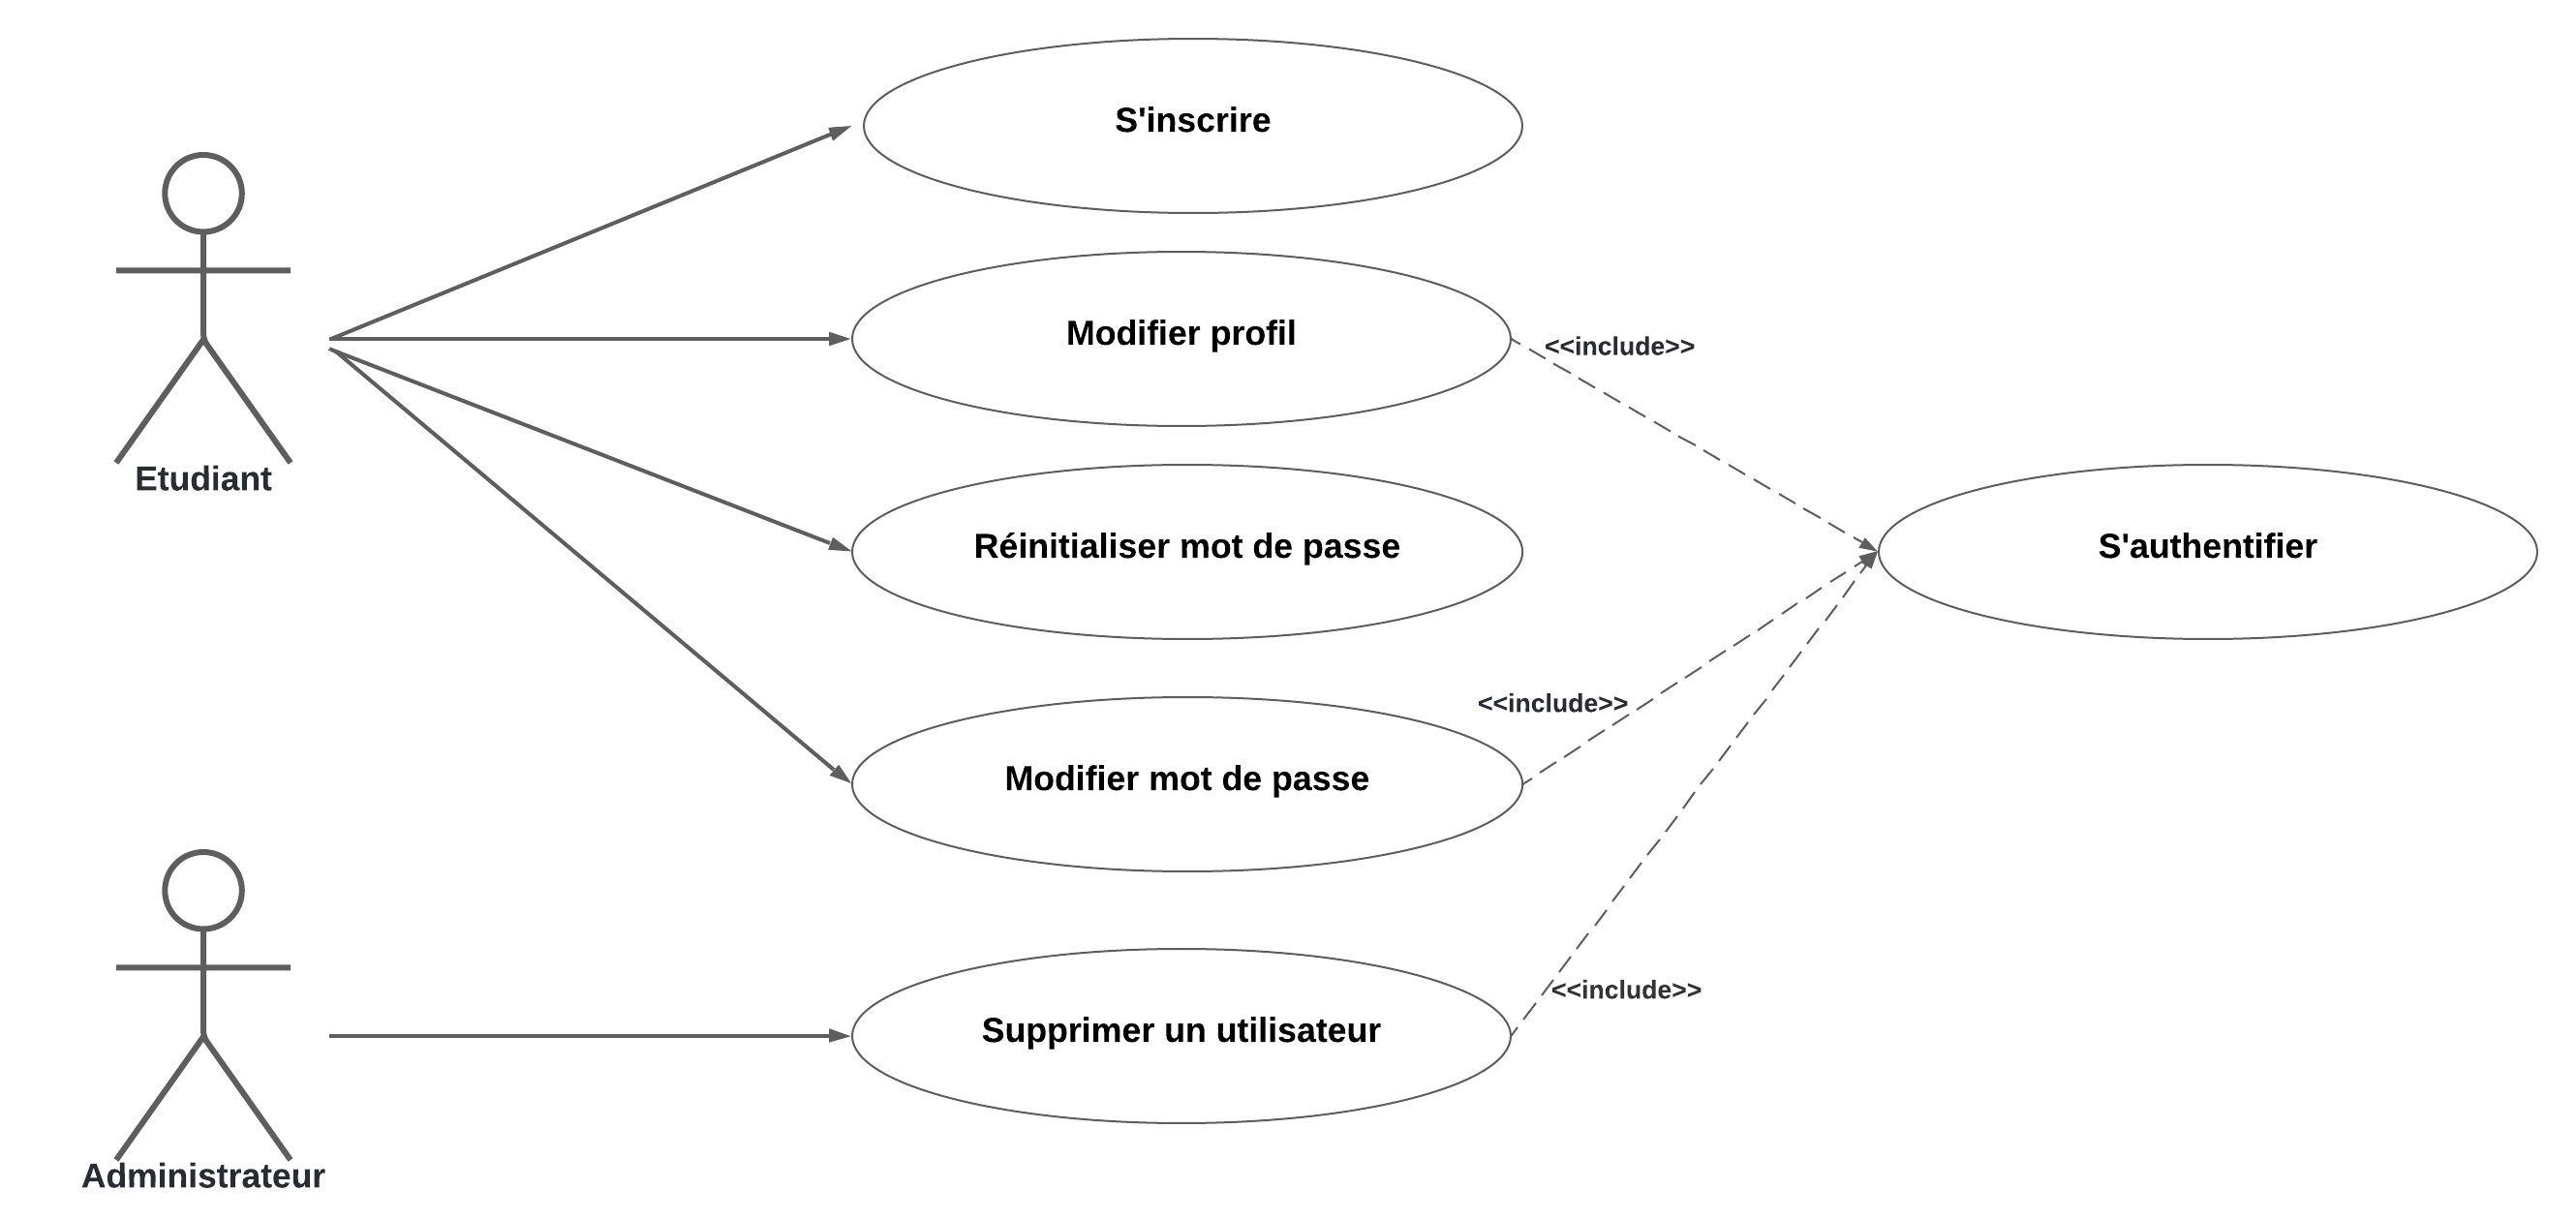
\includegraphics[height=9cm,width=13cm]{images/AAAUseCasesAuthentification.png}%
    }
    \caption{Figure du Diagramme de cas d'utilisation sprint 1}
\end{figure}

\vspace{-1.3cm}
\subsection{Description textuelle du cas d’utilisation « S'inscrire »}
\vspace{-3mm}
Le diagramme ci-dessous illustre le processus d'inscription dans la section mobile de notre application. Cette inscription est une étape essentielle pour accéder aux fonctionnalités de l'application.

\begin{table}[h]
\centering
\begin{tabular}{|p{3cm}|p{12cm}|}
\hline
\textbf{Cas d'utilisation } & S’inscrire  \\
\hline
\textbf{Acteurs} & Étudiant, Admin \\
\hline
\textbf{Précondition} & Non inscrit et non connecté \\
\hline
\textbf{Postcondition} & Inscription validée et succès d‘accès \\
\hline
\textbf{Scénario nominal} & 
\begin{enumerate}
    \item Le système affiche la page de SignUp.
    \item L’acteur saisit son Email et son mot de passe.
    \item L’acteur appuie sur le bouton « S’inscrire ».
    \item L'utilisateur remplit ses informations personnelles.
\end{enumerate} \\
\hline
\textbf{Scénario alternatif} & 
\begin{enumerate}
    \item L’acteur saisit son Email et son mot de passe.
    \item Le système vérifie si l'Email existe déjà.
    \item Si l'Email existe déjà, le système affiche un message d’erreur informant que le compte existe déjà.
\end{enumerate} \\
\hline
\textbf{Exceptions} &  Un champ est vide. Le système affiche un message d’erreur informant qu'il y a des champs à remplir. \\
\hline
\end{tabular}
\caption{Description du cas d’utilisation « S'inscrire »}
\end{table}


\vspace{-9mm}
\subsection{Description textuelle du cas d’utilisation « S’authentifier »}
\vspace{-4mm}
Le diagramme suivant décrit la phase d’authentification dans la partie mobile de notre application. L'authentification est une étape cruciale pour accéder aux fonctionnalités de notre application.
\vspace{5mm}
\begin{table}[h]
\centering
\begin{tabular}{|p{3cm}|p{12cm}|}
\hline
\textbf{Cas d'utilisation} & S’authentifier  \\
\hline
\textbf{Acteurs} & Étudiant, Admin \\
\hline
\textbf{Précondition} & Déjà inscrit mais non connecté \\
\hline
\textbf{Postcondition} & Authentification validée et succès d‘accès \\
\hline
\textbf{Scénario nominal} & 
\begin{enumerate}
    \item Le système affiche la page de connexion.
    \item L’acteur saisit son Email et son mot de passe.
    \item L’acteur appuie sur le bouton « S’identifier ».
    \item Le système vérifie la validité des informations fournies. Si les informations sont incorrectes, alors appel de l’exception.
\end{enumerate} \\
\hline
\textbf{Scénario alternatif} & 
\begin{enumerate}
    \item L’acteur clique sur « Mot de passe oublié ».
    \item Le système affiche une page de récupération de mot de passe.
    \item L’acteur saisit son Email et appuie sur « Envoyer ».
    \item Le système envoie un Email de récupération à l’acteur.
    \item L’acteur clique sur le lien de récupération dans l'Email et saisit un nouveau mot de passe.
    \item Le système enregistre le nouveau mot de passe et affiche une confirmation de succès.
\end{enumerate} \\
\hline
\textbf{Exception} & 
\begin{enumerate}
    \item Login et/ou mot de passe incorrect(s).
    \item Le système affiche un message d’erreur informant l’utilisateur que son login ou mot de passe est incorrect.
\end{enumerate} \\
\hline
\end{tabular}
\caption{Description du cas d’utilisation « S'authentifier »}
\end{table}

\vspace{-1cm}
\subsection{Description textuelle du cas d’utilisation « Modifier le profil »}
\vspace{-4mm}
Le diagramme suivant présente le processus de modification de profil dans la partie mobile de notre application. Cette étape implique deux acteurs : l'étudiant et l'admin.
\begin{table}[h]
\centering
\begin{tabular}{|p{3cm}|p{12cm}|}
\hline
\textbf{Cas d'utilisation } & Modifier le profil  \\
\hline
\textbf{Acteurs} & Etudiant, Admin \\
\hline
\textbf{Précondition} & Acteurs authentifiés \\
\hline
\textbf{Postcondition} & Modification validée \\
\hline
\textbf{Scénario nominal} &
\begin{enumerate}
    \item Le système affiche l’interface de modification.
    \item L’acteur saisit ses informations personnelles.
    \item Le système modifie le profil.
    \item Le système affiche un message de succès.
\end{enumerate} \\
\hline
\end{tabular}
\caption{Description du cas d’utilisation « Modifier le profil »}
\end{table}


\vspace{0cm}
\subsection{Description textuelle du cas d’utilisation « Modifier mot de passe »}
\vspace{-4mm}
Le diagramme ci-dessous présente le déroulement de la modification du mot de passe dans la section mobile de notre application. Deux acteurs doivent participer à cette étape : l'étudiant et l'admin.

\begin{table}[h]
\centering
\begin{tabular}{|p{3cm}|p{12cm}|}
\hline
\textbf{Cas d'utilisation } & Modifier mot de passe  \\
\hline
\textbf{Acteurs} & Etudiant, Admin \\
\hline
\textbf{Précondition} & Acteurs authentifiés \\
\hline
\textbf{Postcondition} & Mot de passe modifié \\
\hline
\textbf{Scénario nominal} &
\begin{enumerate}
    \item L’acteur clique sur le bouton « modifier le mot de passe ».
    \item Le système affiche l’interface de modification de mot de passe.
    \item L’acteur saisit et confirme son nouveau mot de passe. Si le mot de passe est invalide .
    \item Le système affiche un message de succès.
\end{enumerate} \\
\hline
\textbf{Exception } & Mot de passe vide ou ne répond pas aux exigences. \\
& Le système affiche un message d’erreur. \\
\hline
\end{tabular}
\caption{Description du cas d’utilisation « Modifier mot de passe »}
\end{table}

\vspace{-1.2cm}
\section{Diagramme de séquence }
\vspace{-4mm}

Les diagrammes de séquence décrivent de manière séquentielle les interactions entre l'utilisateur et le système lors de la gestion des utilisateurs.

\vspace{-9mm}
\subsection{Diagramme de séquence « S’inscrire »}
\vspace{-4mm}
Ce diagramme de séquence montre le processus par lequel un utilisateur s'inscrit dans un système. Il met en évidence les interactions entre l'utilisateur et le système nécessaires pour finaliser l'inscription.
\vspace{-4mm}
\begin{figure}[H]%
    \center%
    \setlength{\fboxsep}{5pt}%
    \setlength{\fboxrule}{0.5pt}%
    \fbox{
    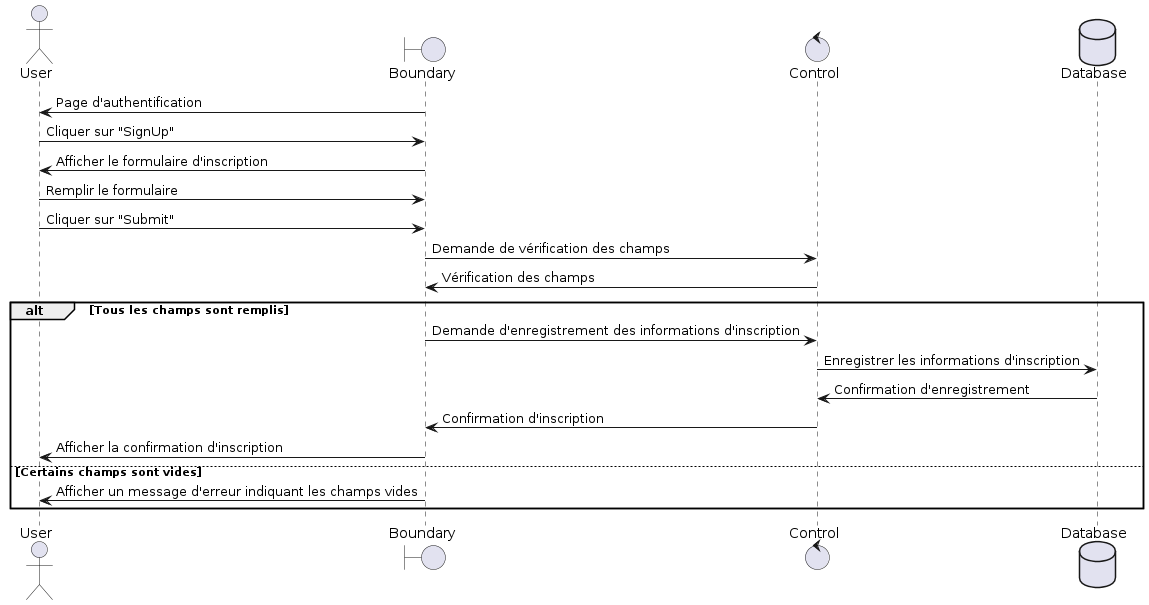
\includegraphics[height=8cm,width=15cm]{images/ffsignupp.png}%
    }
    \caption{Figure du Diagramme de sequence «s'inscrire»  }
\end{figure}
\vspace{-1.3cm}
\subsection{Diagramme de séquence « S’authentifier »}
\vspace{-4mm}
Ce diagramme de séquence illustre le processus d'authentification d'un utilisateur dans un système. Il décrit les interactions entre l'utilisateur et le système lors de la tentative de connexion avec un email et un mot de passe.
\vspace{-4mm}
\begin{figure}[H]%
    \center%
    \setlength{\fboxsep}{5pt}%
    \setlength{\fboxrule}{0.5pt}%
    \fbox{
    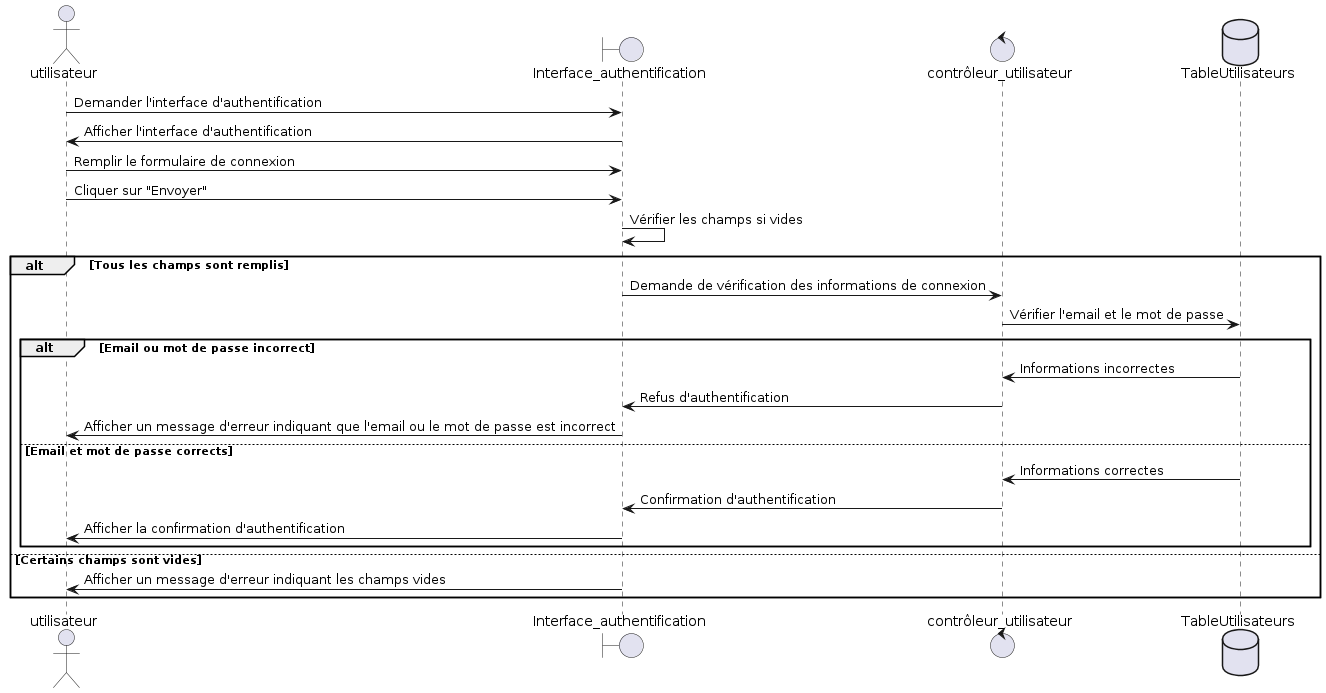
\includegraphics[height=10cm,width=15cm]{images/ffffloginX.png}%
    }
    \caption{Figure du Diagramme de sequence « s'authentifier » }
\end{figure}
\vspace{-1.3cm}
\subsection{Diagramme de séquence « Changer mot de passe »}
\vspace{-4mm}
Ce diagramme de séquence décrit le processus par lequel un utilisateur change son mot de passe dans un système. Il montre en détail les interactions entre l'utilisateur et le système nécessaires pour accomplir cette tâche.
\begin{figure}[H]%
    \center%
    \setlength{\fboxsep}{5pt}%
    \setlength{\fboxrule}{0.5pt}%
    \fbox{
    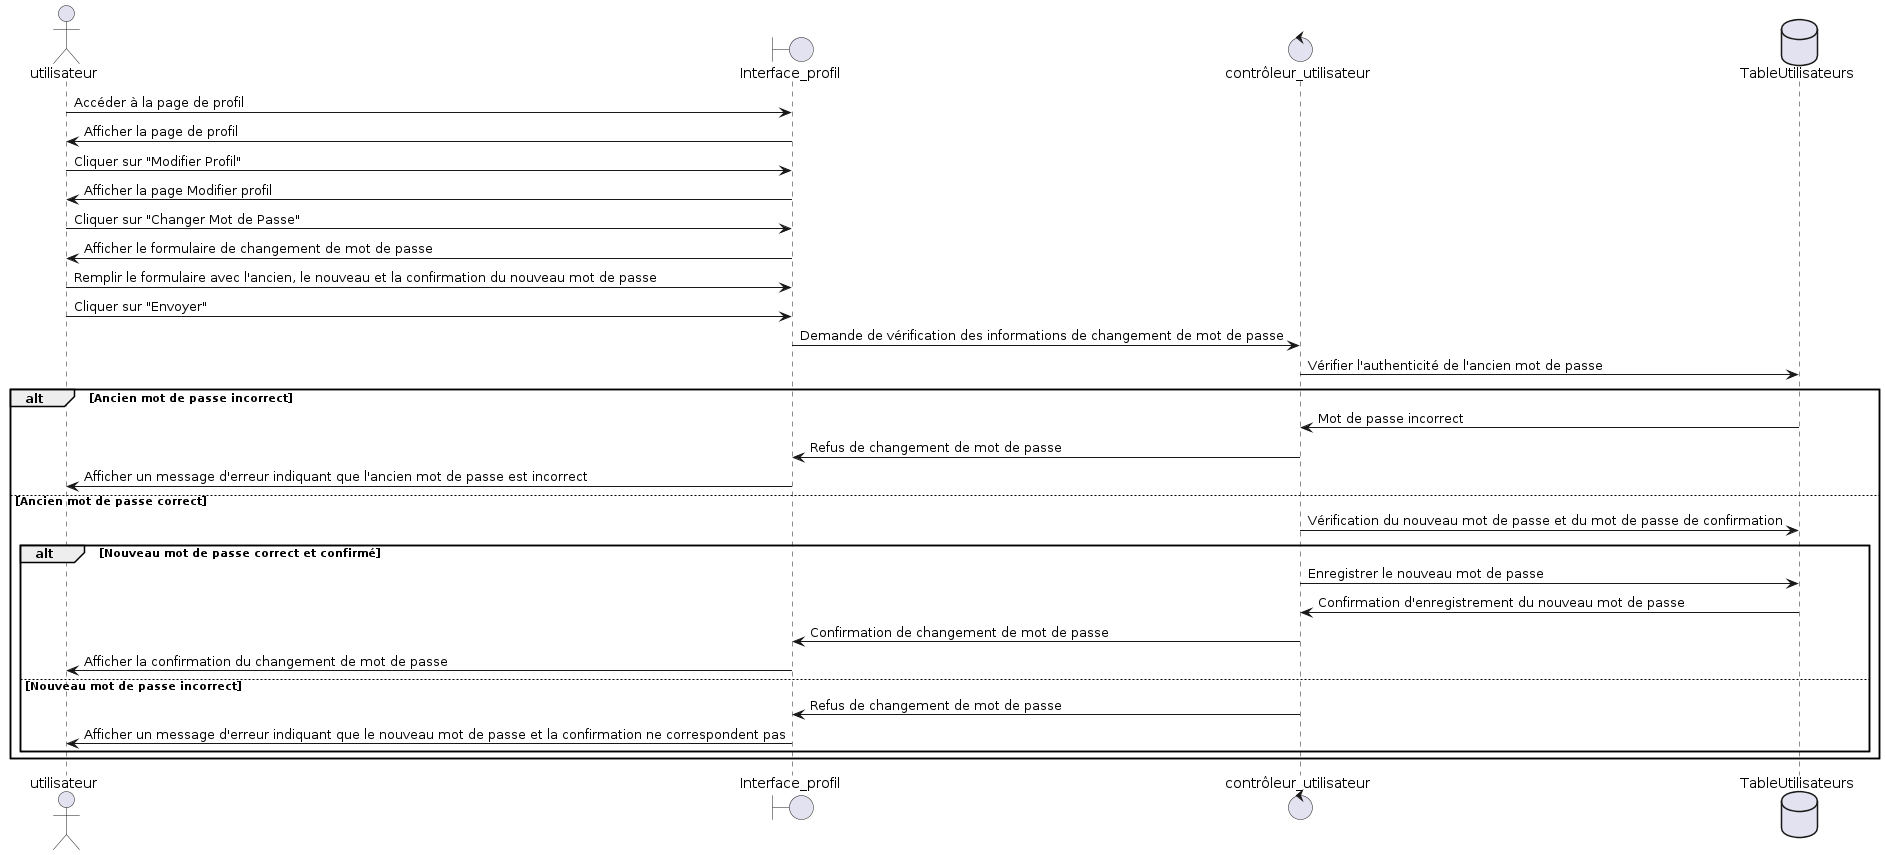
\includegraphics[height=15cm,width=15cm]{images/ffchangermotdepasseee.png}%
    }
    \caption{Figure du Diagramme de sequence «Changer mot de passe» }
\end{figure}
\vspace{-1.2cm}
\section{Diagramme de classes}
\vspace{-4mm}
Le diagramme de classes est un élément principal de conception d’un logiciel, c’est un modèle représentant la structure du système à concevoir. Le diagramme de classes est un schéma utilisé pour présenter les classes et les différentes relations. 
\begin{figure}[H]%
    \center%
    \setlength{\fboxsep}{5pt}%
    \setlength{\fboxrule}{0.5pt}%
    \fbox{
    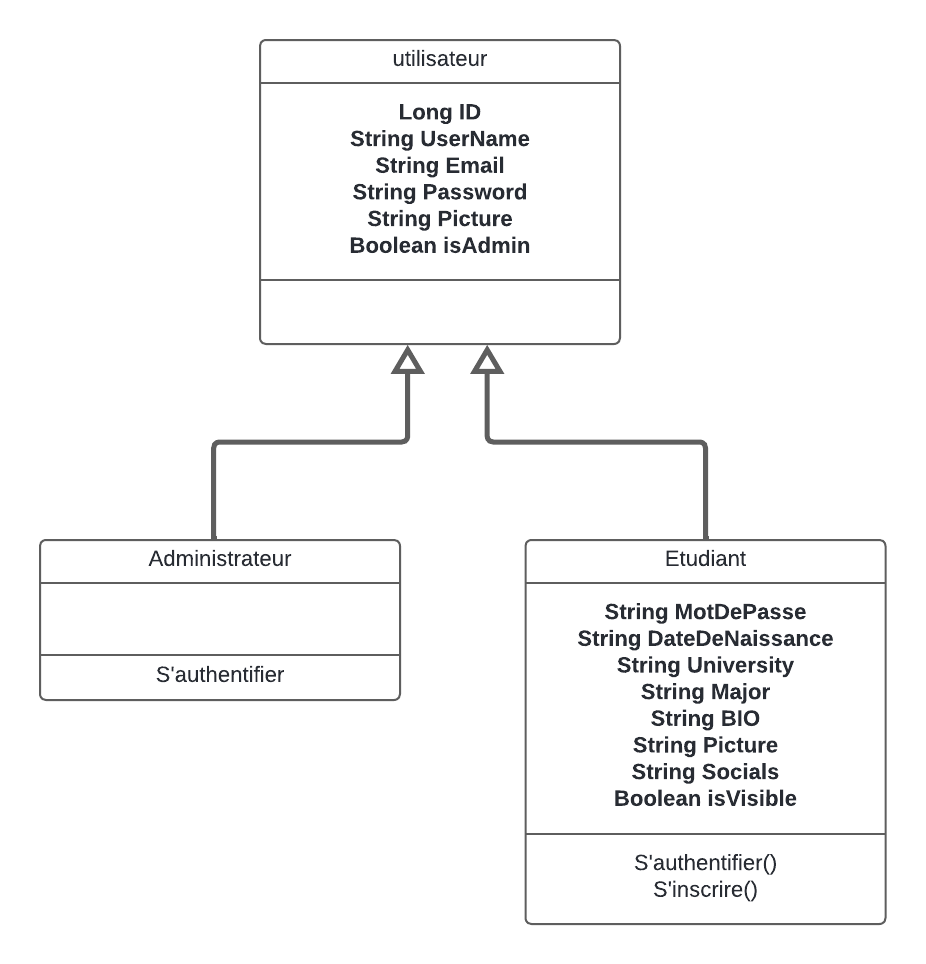
\includegraphics[height=17cm,width=15cm]{images/AAAAuthentification.png}%
    }
    \caption{Figure du Diagramme de classes Sprint 1}
\end{figure}
\vspace{-1.5cm}
\section{Réalisation }
\vspace{-4mm}
La partie de réalisation représente la dernière phase du cycle de développement d’un sprint. Elle permet de présenter les résultats obtenus lors de l’étape de développement afin d’assurer et de garantir une version de qualité.
\vspace{-7mm}
\subsection{Authentification}
\vspace{-3mm}
L’interface d’authentification, c’est la première interface vue par l’utilisateur.
\begin{figure}[H]%
    \center%
    \setlength{\fboxsep}{5pt}%
    \setlength{\fboxrule}{0.5pt}%
    \fbox{
    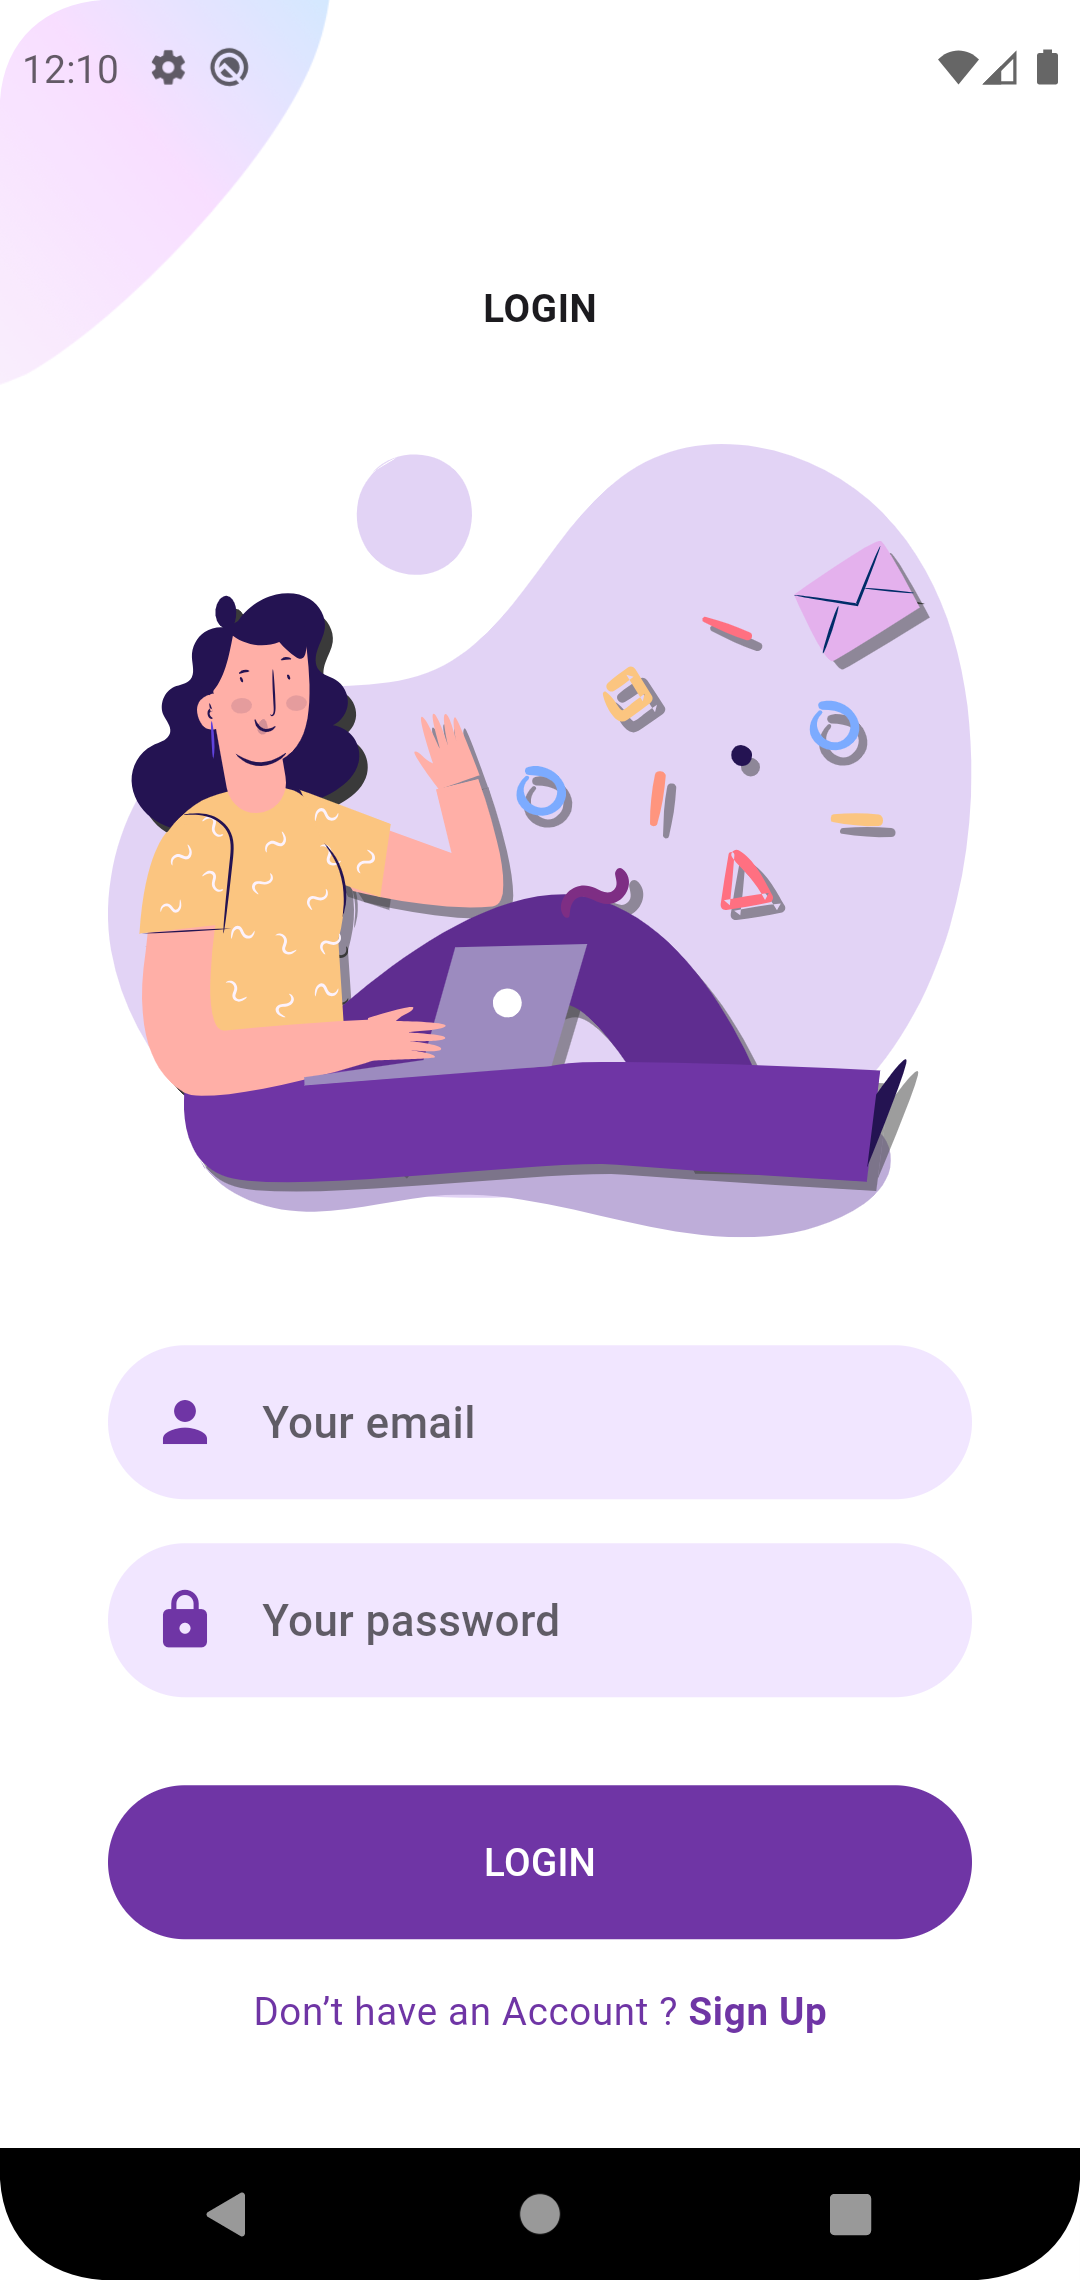
\includegraphics[height=9.5cm,width=7cm]{images/loginPage.png}%
    }
    \caption{Interface Login mobile}
\end{figure}
\vspace{-1.2cm}
\subsection{Authentification web}
\vspace{-4mm}
L’interface d’authentification pour la partie web, c’est la première interface vue par l’admin.
\vspace{-6mm}
\begin{figure}[H]%
    \center%
    \setlength{\fboxsep}{5pt}%
    \setlength{\fboxrule}{0.5pt}%
    \fbox{
    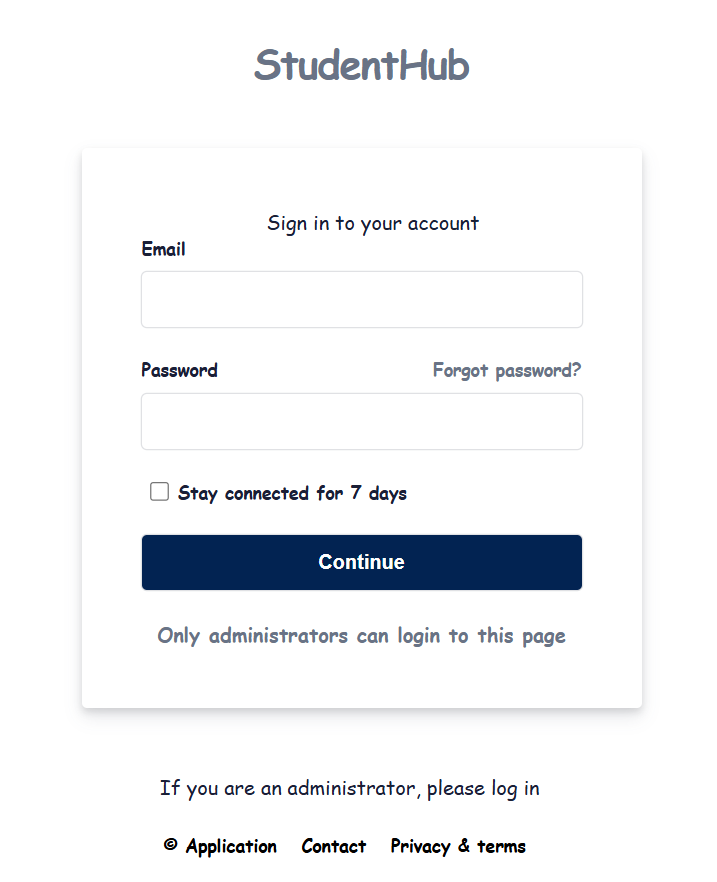
\includegraphics[height=9.5cm,width=12cm]{images/AdminLoginPage.png}%
    }
    \caption{Interface Login web }
\end{figure}

\subsection{Inscription}
\vspace{-4mm}
La page d'inscription permet aux nouveaux utilisateurs de créer leur compte facilement.
\begin{figure}[H]
    \centering

    \begin{subfigure}{0.45\textwidth}
        \centering
        \setlength{\fboxsep}{5pt}%
        \setlength{\fboxrule}{0.5pt}%
        \fbox{
            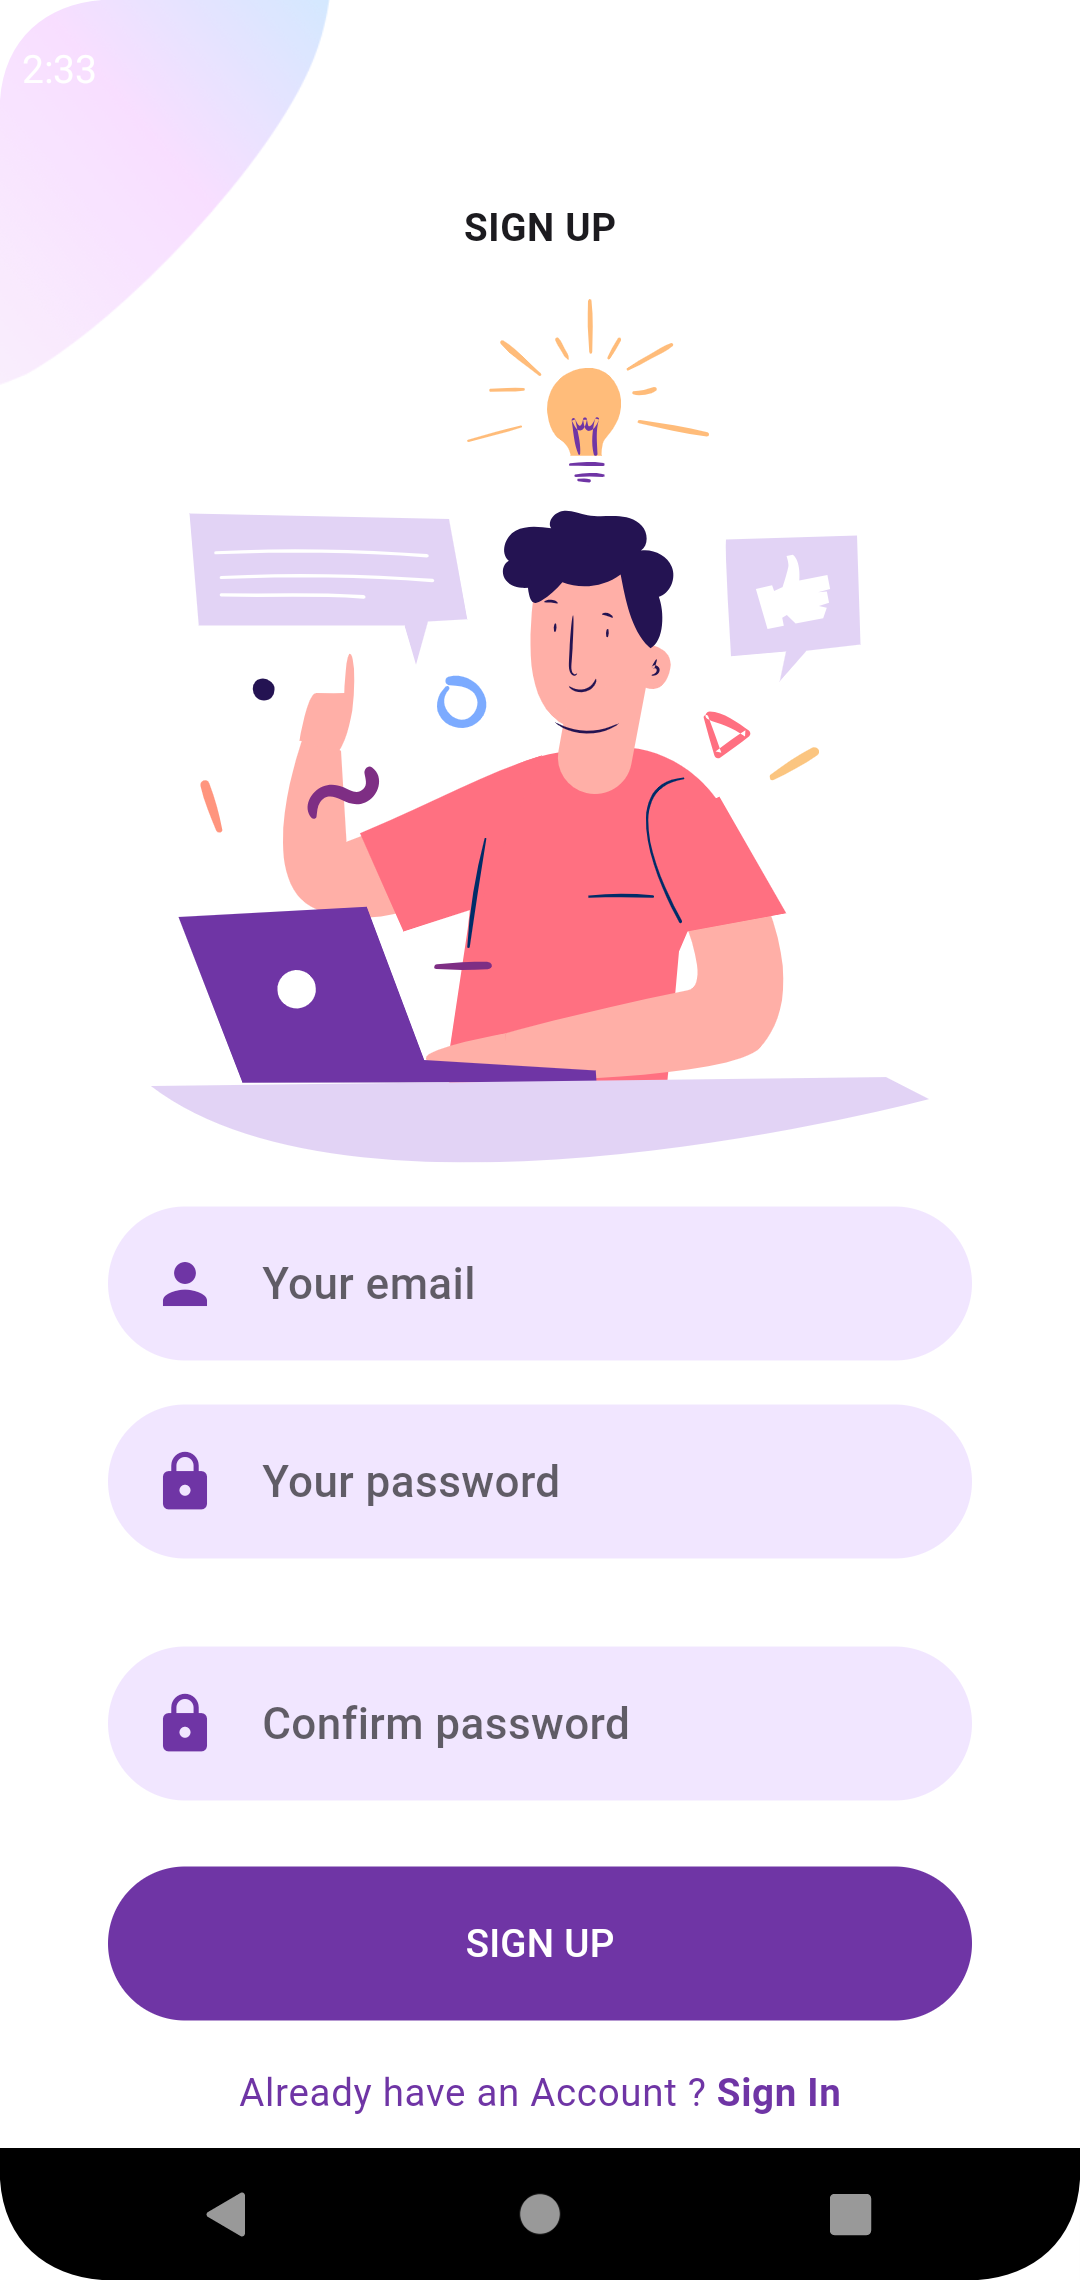
\includegraphics[height=9.5cm,width=7cm]{images/SignUpPage.png}
        }
        \label{fig:first}
    \end{subfigure}
    \hfill
    \begin{subfigure}{0.45\textwidth}
        \centering
        \setlength{\fboxsep}{5pt}%
        \setlength{\fboxrule}{0.5pt}%
        \fbox{
            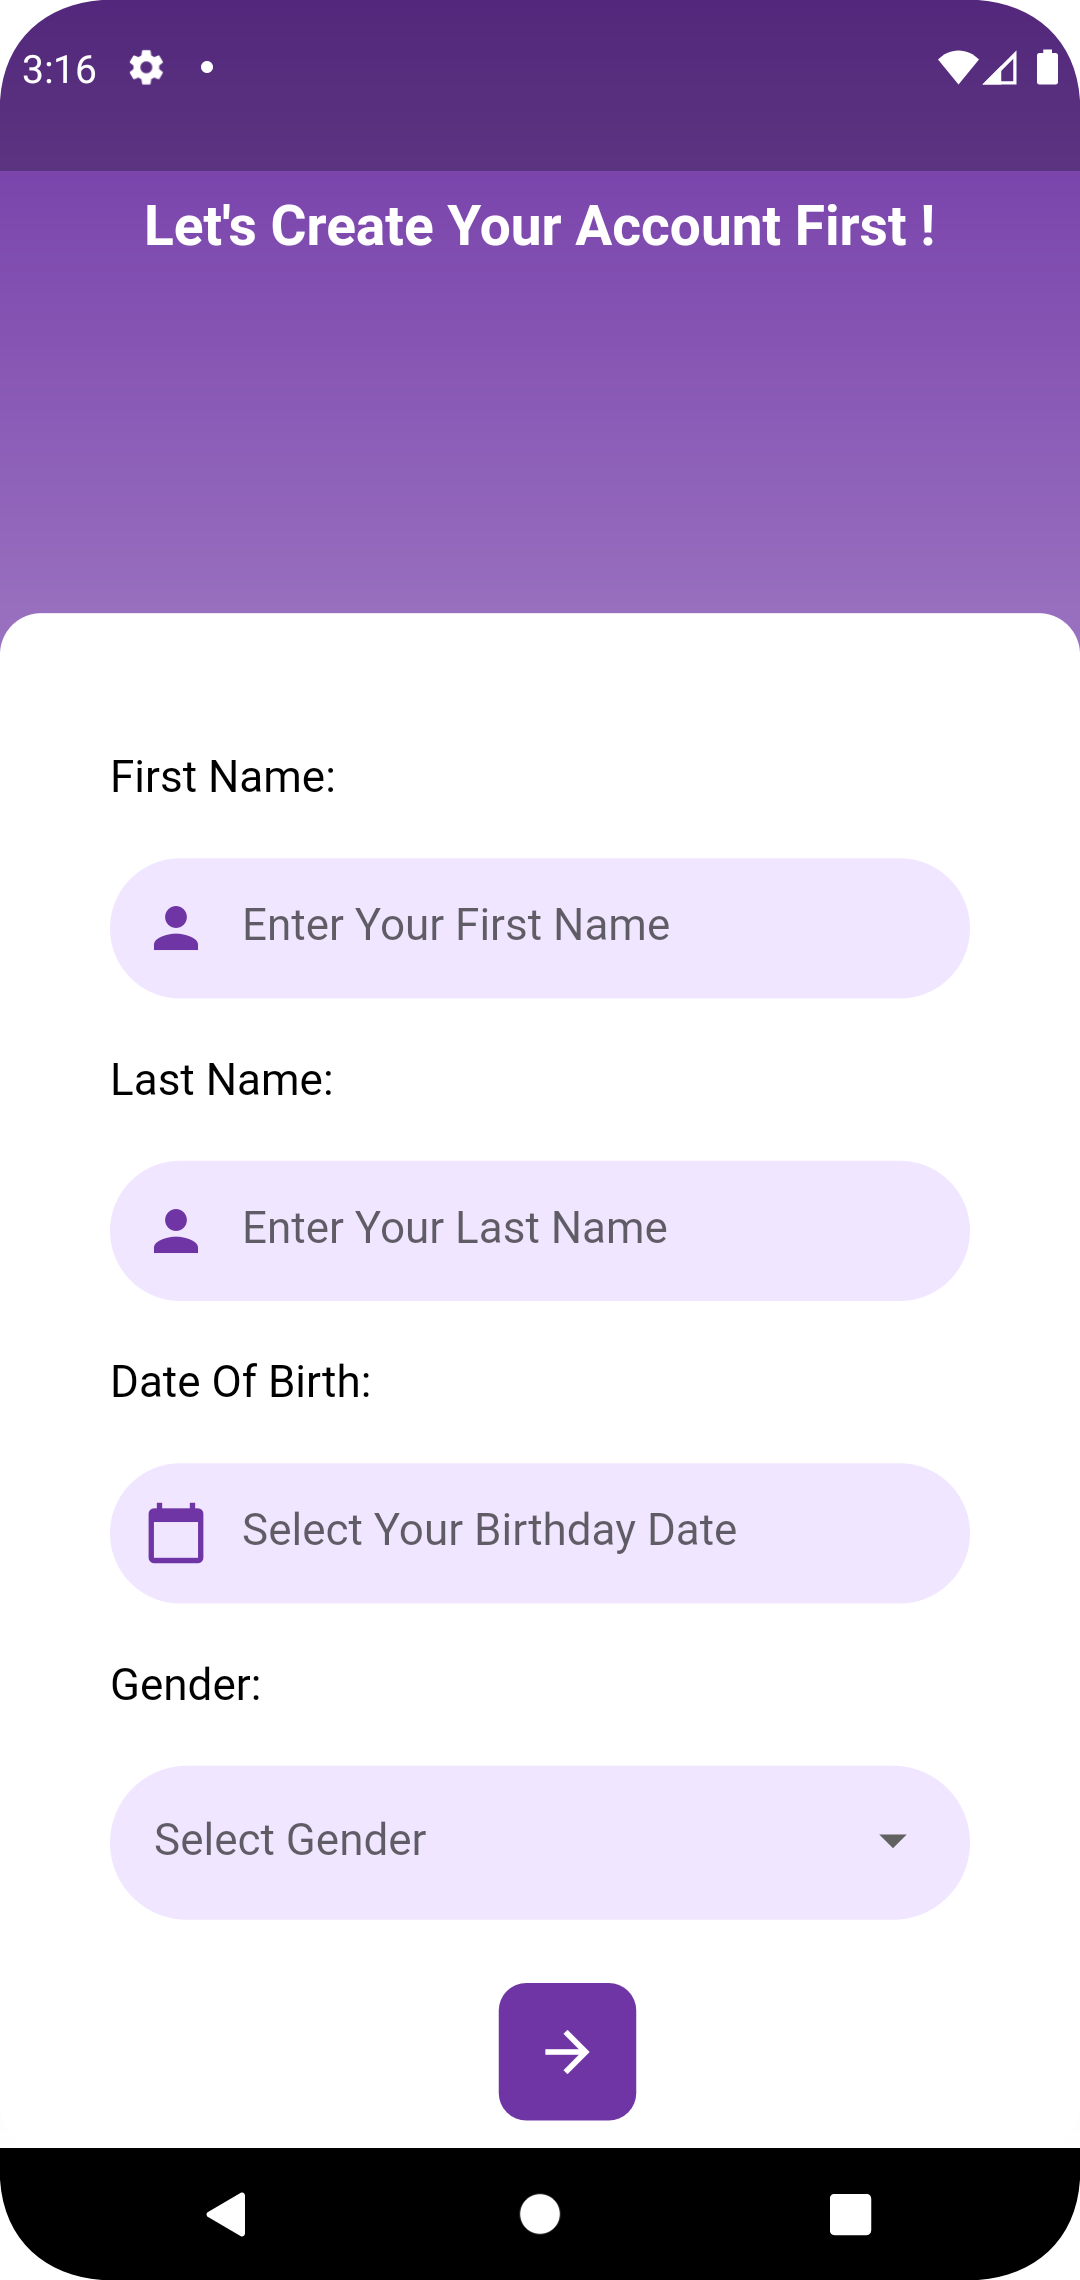
\includegraphics[height=9.5cm,width=7cm]{images/signup1.png}
        }
        \label{fig:second}
    \end{subfigure}
    
    \vspace{0.5cm}
    
    \begin{subfigure}{0.45\textwidth}
        \centering
        \setlength{\fboxsep}{5pt}%
        \setlength{\fboxrule}{0.5pt}%
        \fbox{
            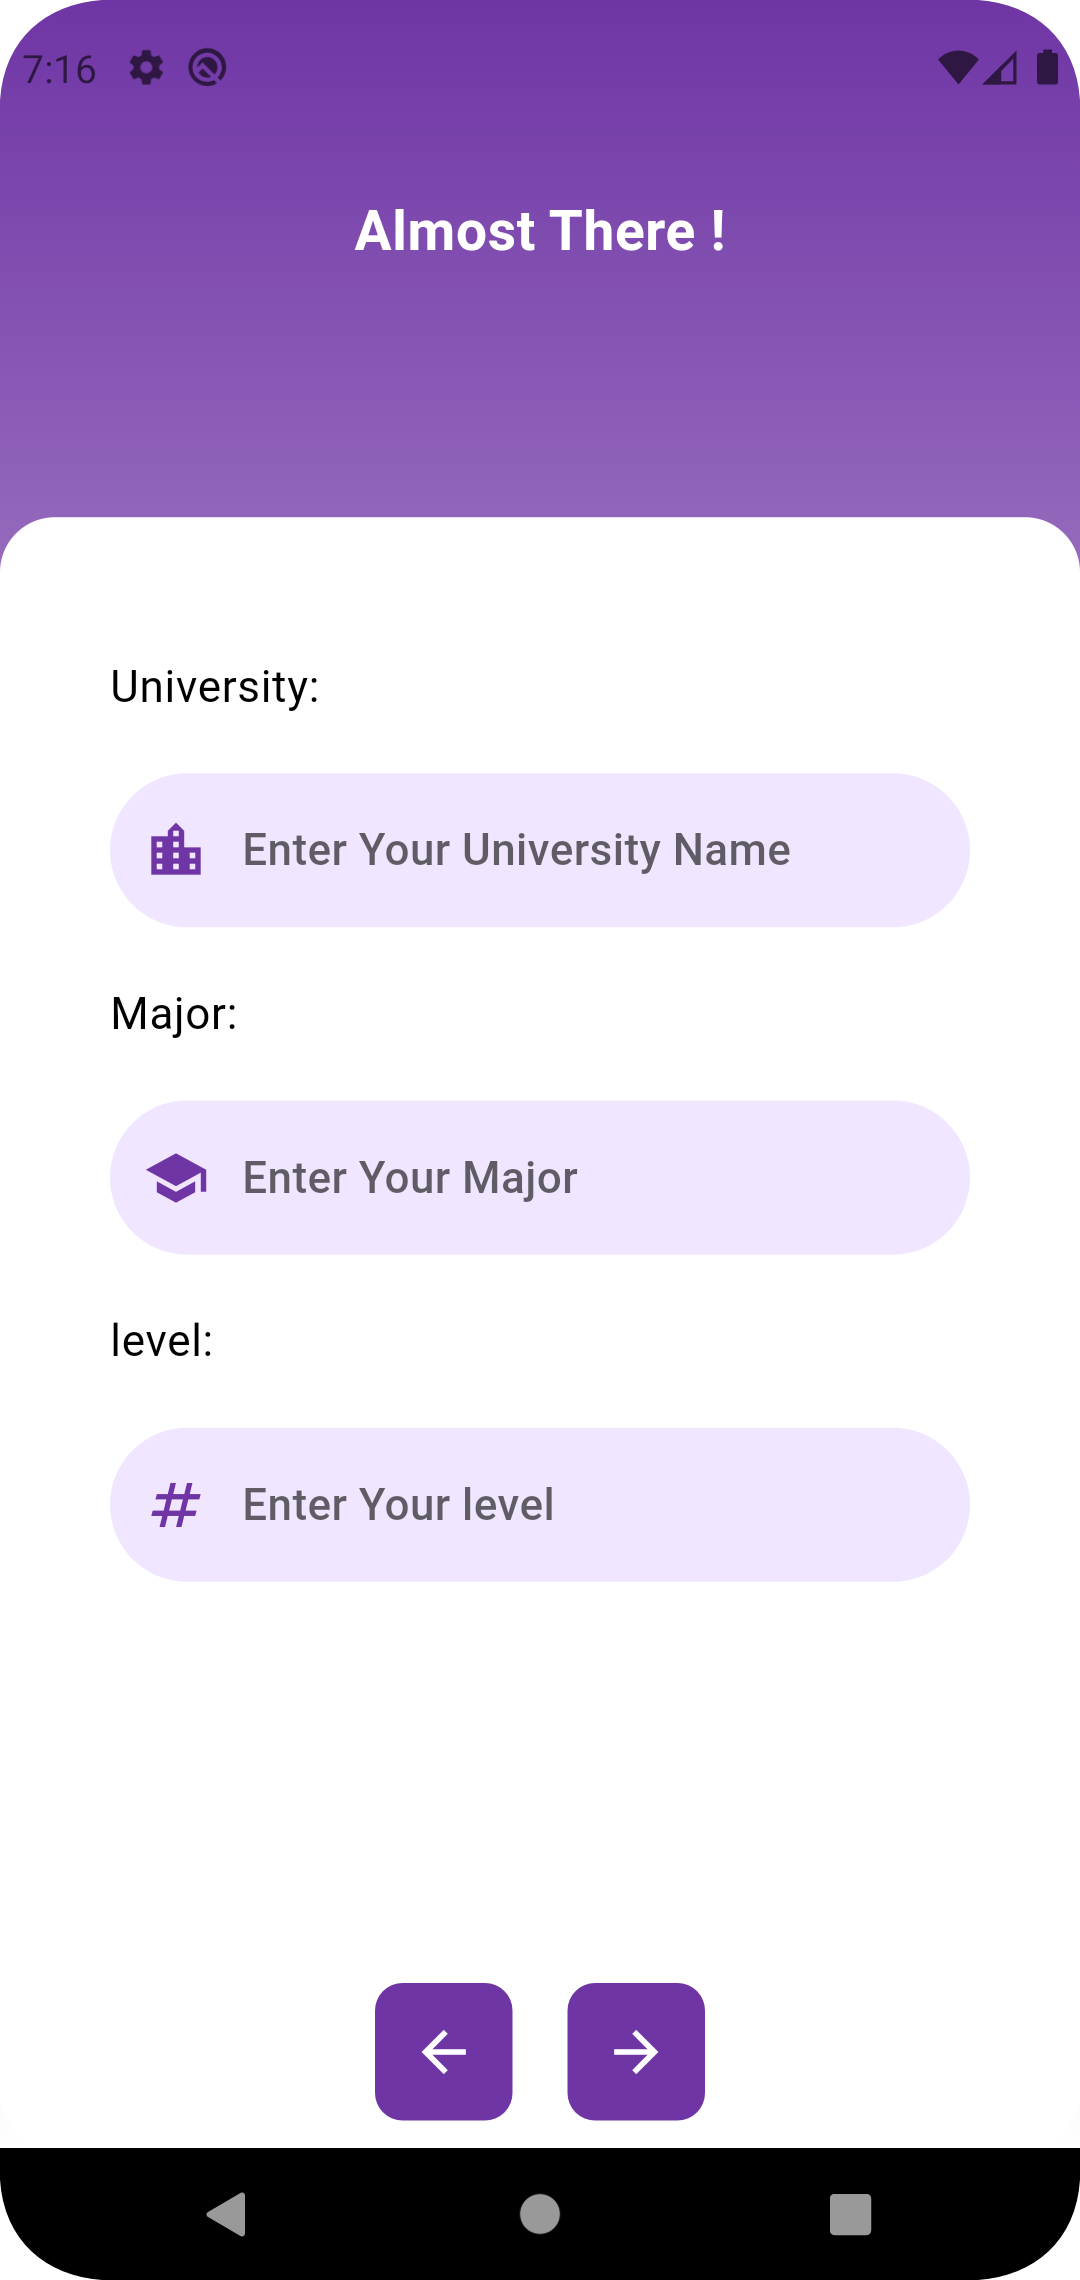
\includegraphics[height=9.5cm,width=7cm]{images/SignUpPage3.png}
        }
        \label{fig:third}
    \end{subfigure}
    \hfill
    \begin{subfigure}{0.45\textwidth}
        \centering
        \setlength{\fboxsep}{5pt}%
        \setlength{\fboxrule}{0.5pt}%
        \fbox{
            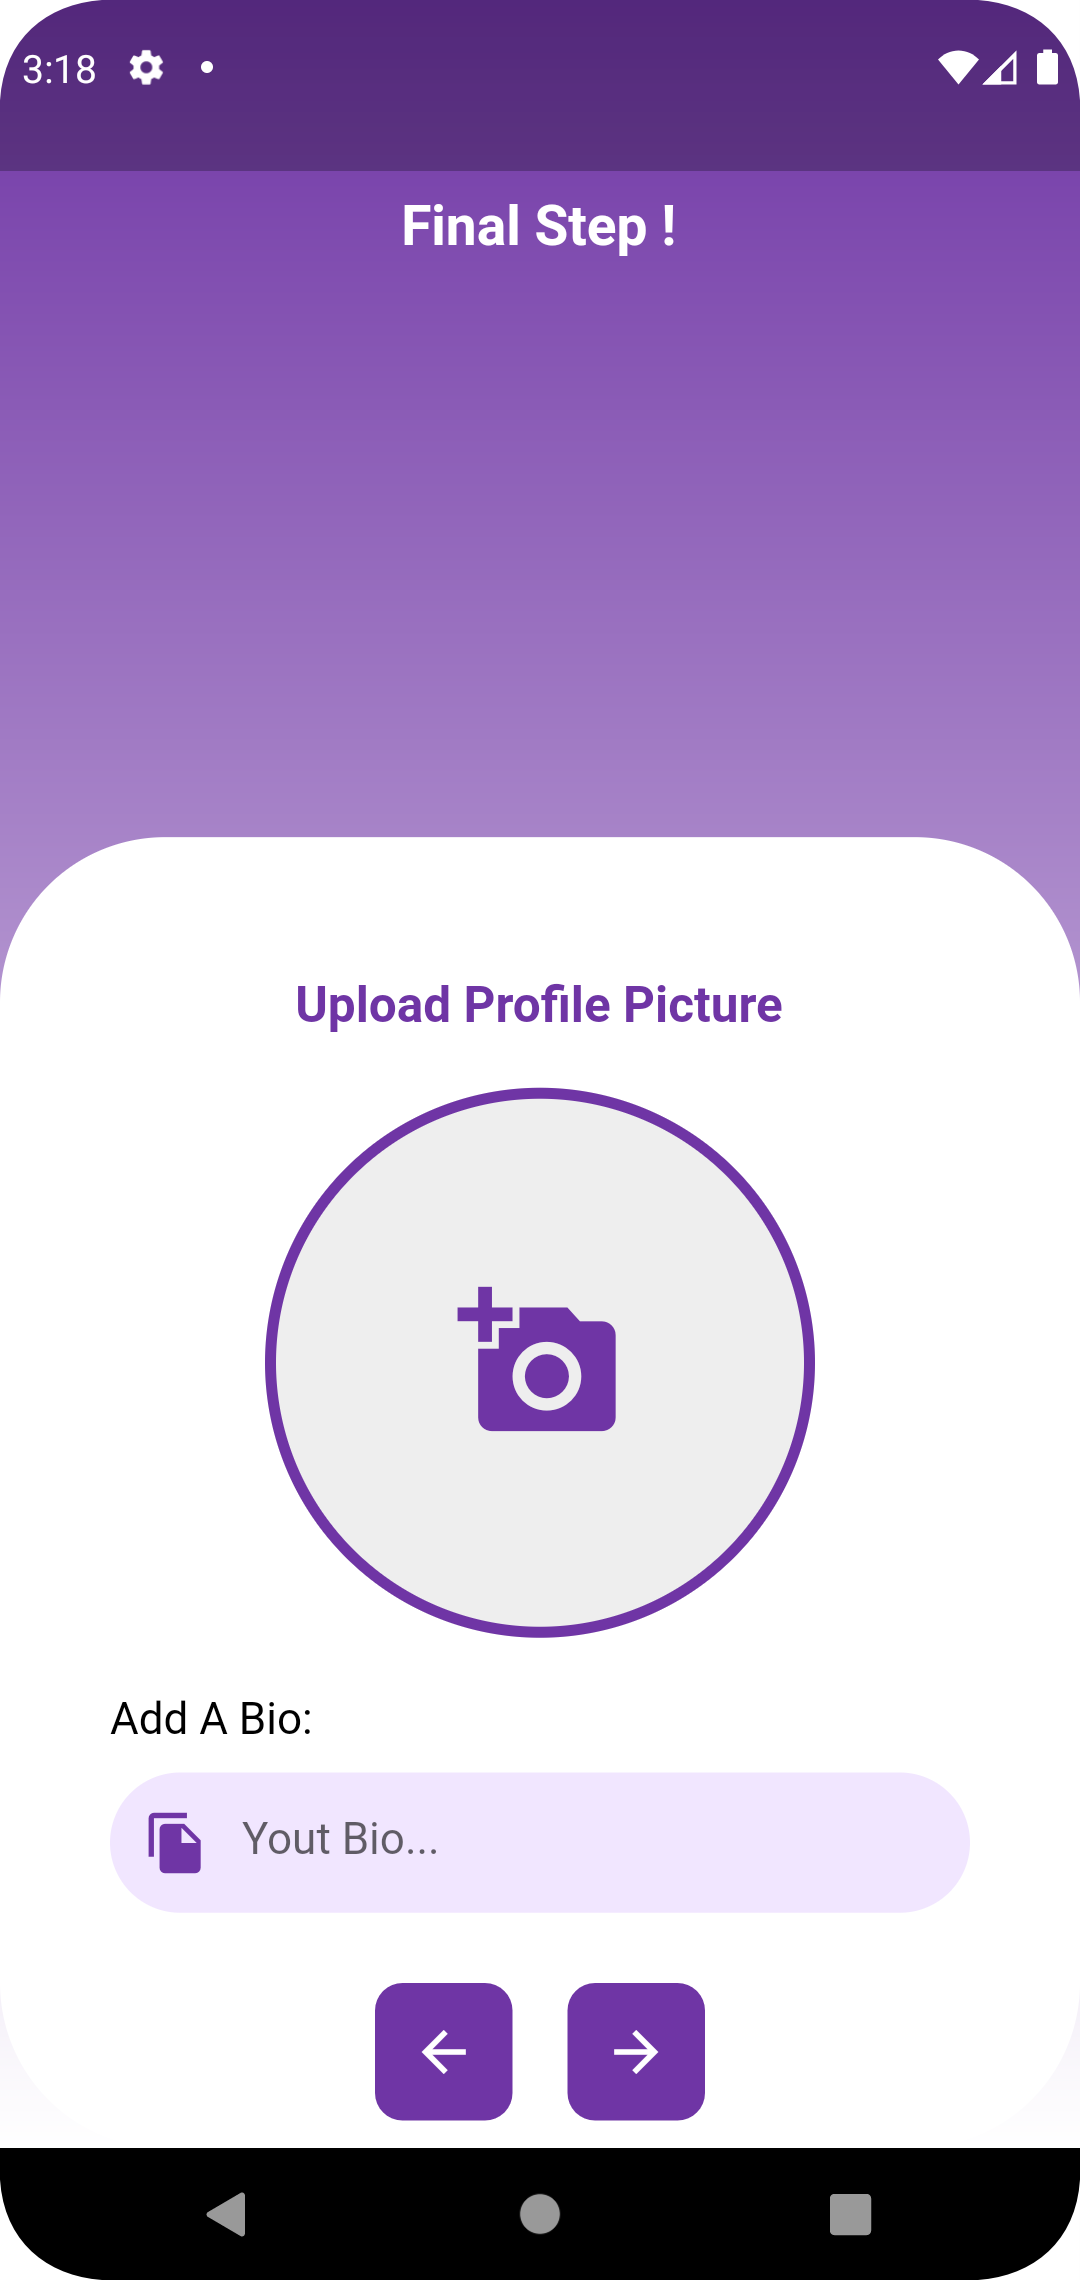
\includegraphics[height=9.5cm,width=7cm]{images/signup3.png}
        }
        \label{fig:fourth}
    \end{subfigure}

    \caption{Les Interfaces du formulaire SignUp}
    \label{fig:all}
\end{figure}



\newpage
\vspace{-8mm}
\subsection{Modifier profile}
\vspace{-6mm}
La page de modification du profil permet aux utilisateurs de mettre à jour leurs informations personnelles en quelques étapes simples, assurant ainsi l'exactitude des données de leur compte.
\vspace{-10mm}
\begin{figure}[H]%
    \center%
    \setlength{\fboxsep}{5pt}%
    \setlength{\fboxrule}{0.5pt}%
    \fbox{
    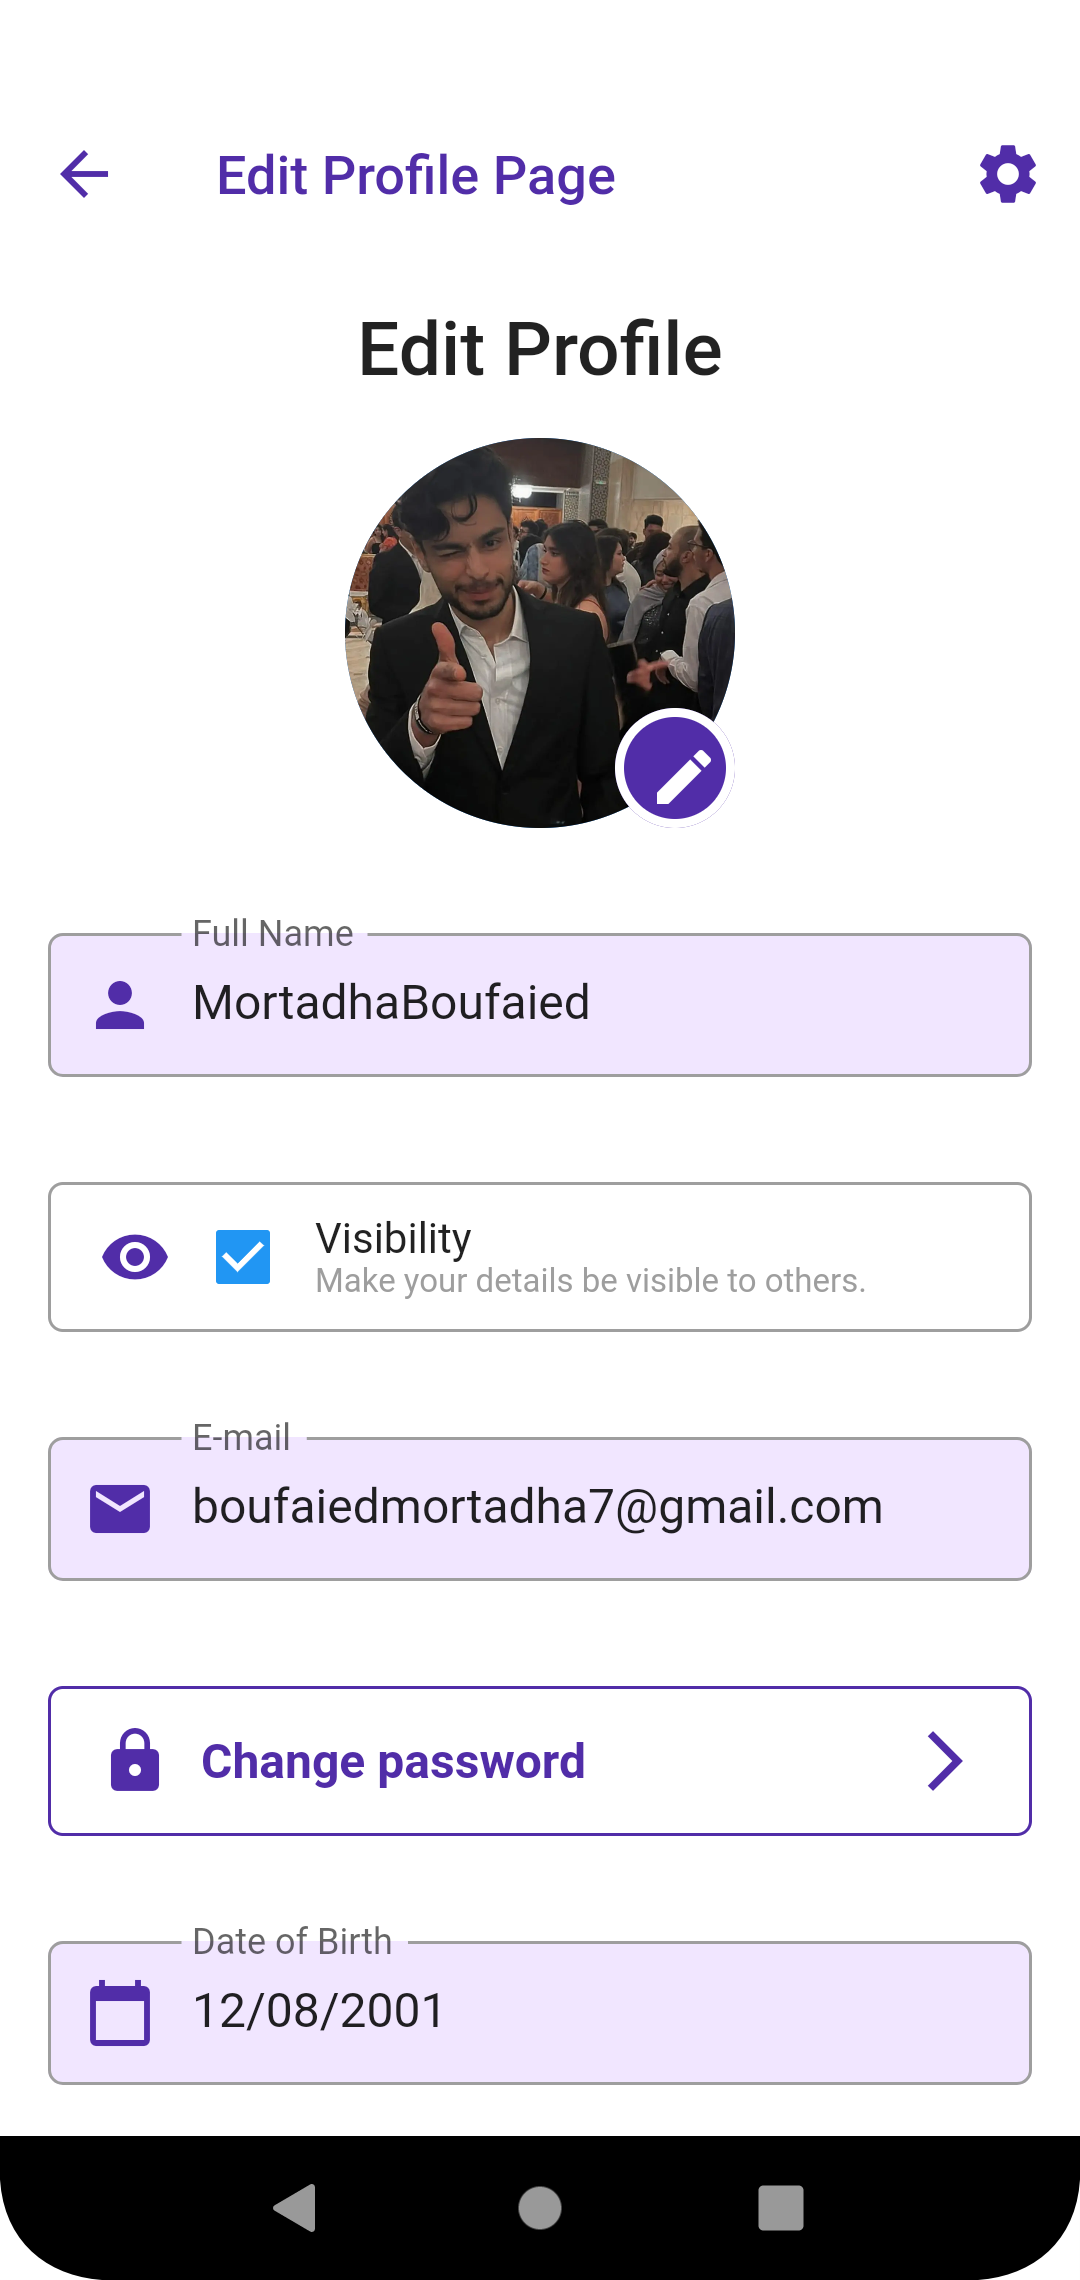
\includegraphics[height=9cm,width=7cm]{images/AAAEditProfile.png}%
    }
    \caption{Interface modifier profile }
\end{figure}
\vspace{-1.8cm}

\subsection{Changer mot de passe}
\vspace{-6mm}
La page permet de changer le mot de passe rapidement pour sécuriser le compte.
\vspace{-2mm}
\begin{figure}[H]%
    \center%
    \setlength{\fboxsep}{5pt}%
    \setlength{\fboxrule}{0.5pt}%
    \fbox{
    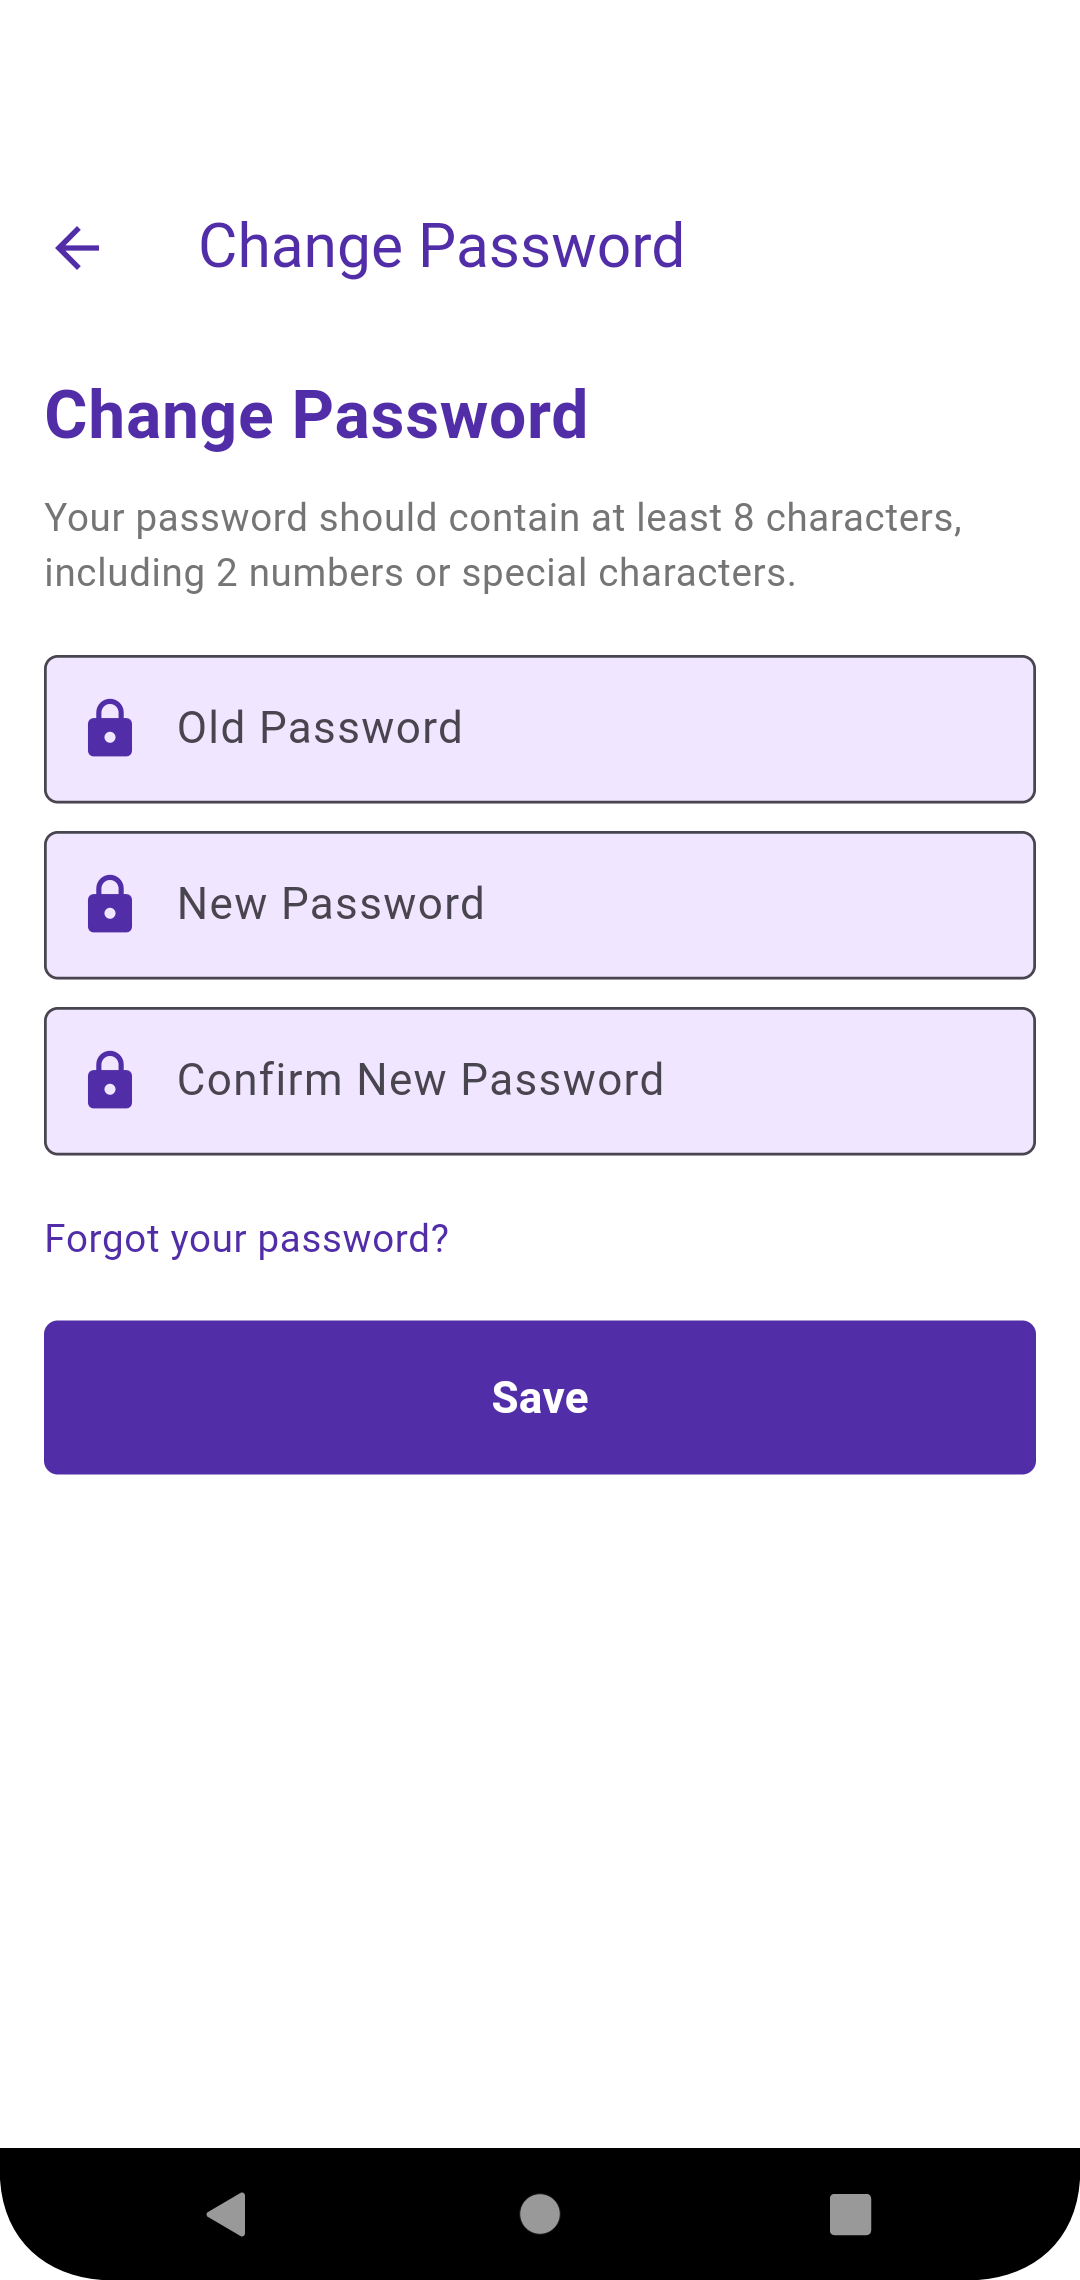
\includegraphics[height=9cm,width=7cm]{images/ChangePassword.png}%
    }
    \caption{Interface changer mot passe }
\end{figure}

\vspace{-4mm}

\subsection{Réinitialiser mot de passe}
\vspace{-4mm}
La réinitialisation du mot de passe permet aux utilisateurs de regagner l'accès à leur compte en cas d'oubli. Ils reçoivent un lien par e-mail pour réinitialiser leur mot de passe et choisir un nouveau en quelques clics.
\begin{figure}[H]
    \centering

    % Première ligne avec deux images côte à côte
    \begin{subfigure}{0.45\textwidth}
        \centering
        \setlength{\fboxsep}{5pt}%
        \setlength{\fboxrule}{0.5pt}%
        \fbox{
            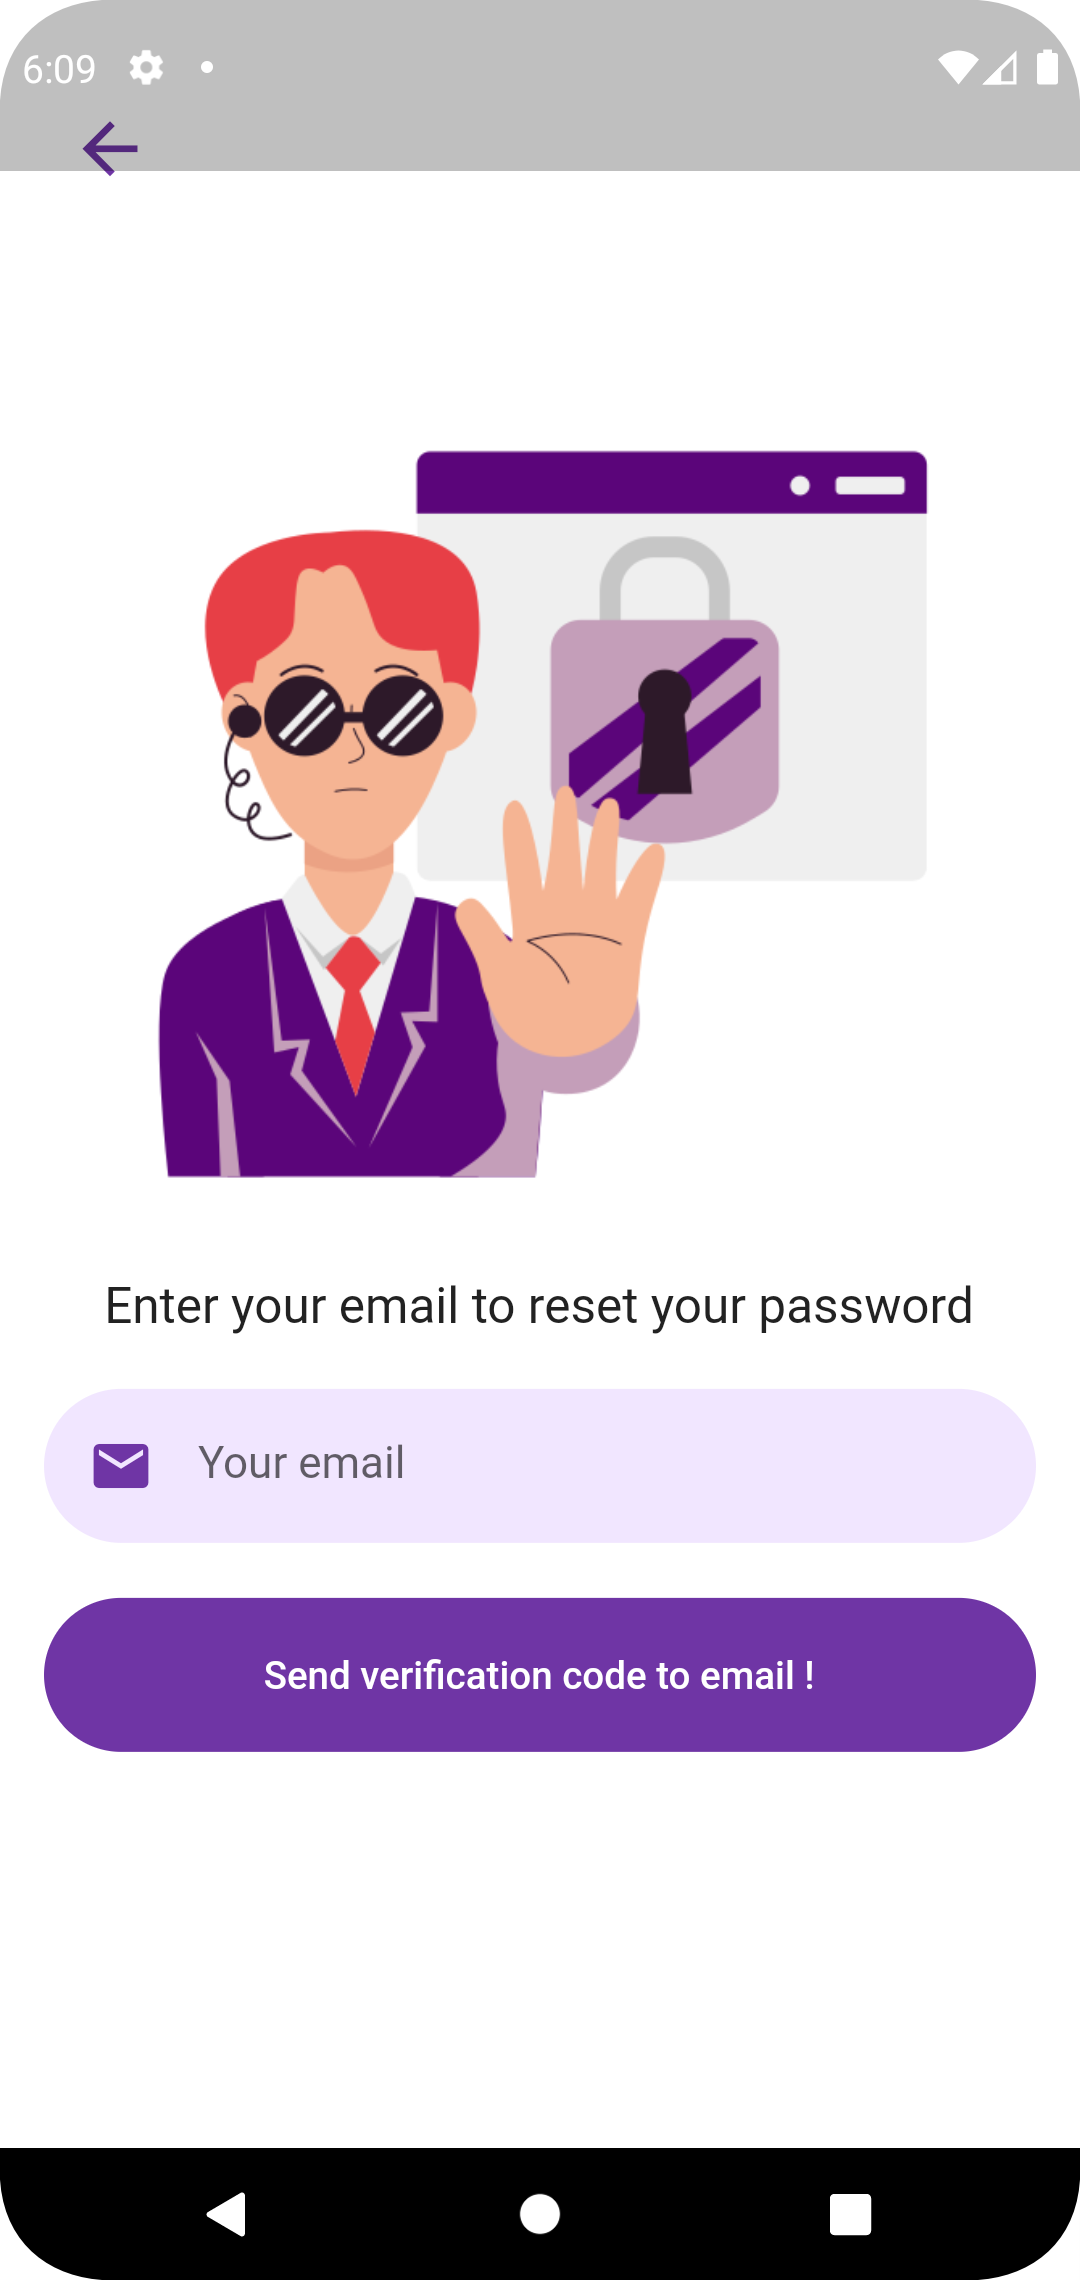
\includegraphics[height=9.2cm,width=7cm]{images/ForgetPassword1.png}
        }
        \label{fig:first}
    \end{subfigure}
    \hfill
    \begin{subfigure}{0.45\textwidth}
        \centering
        \setlength{\fboxsep}{5pt}%
        \setlength{\fboxrule}{0.5pt}%
        \fbox{
            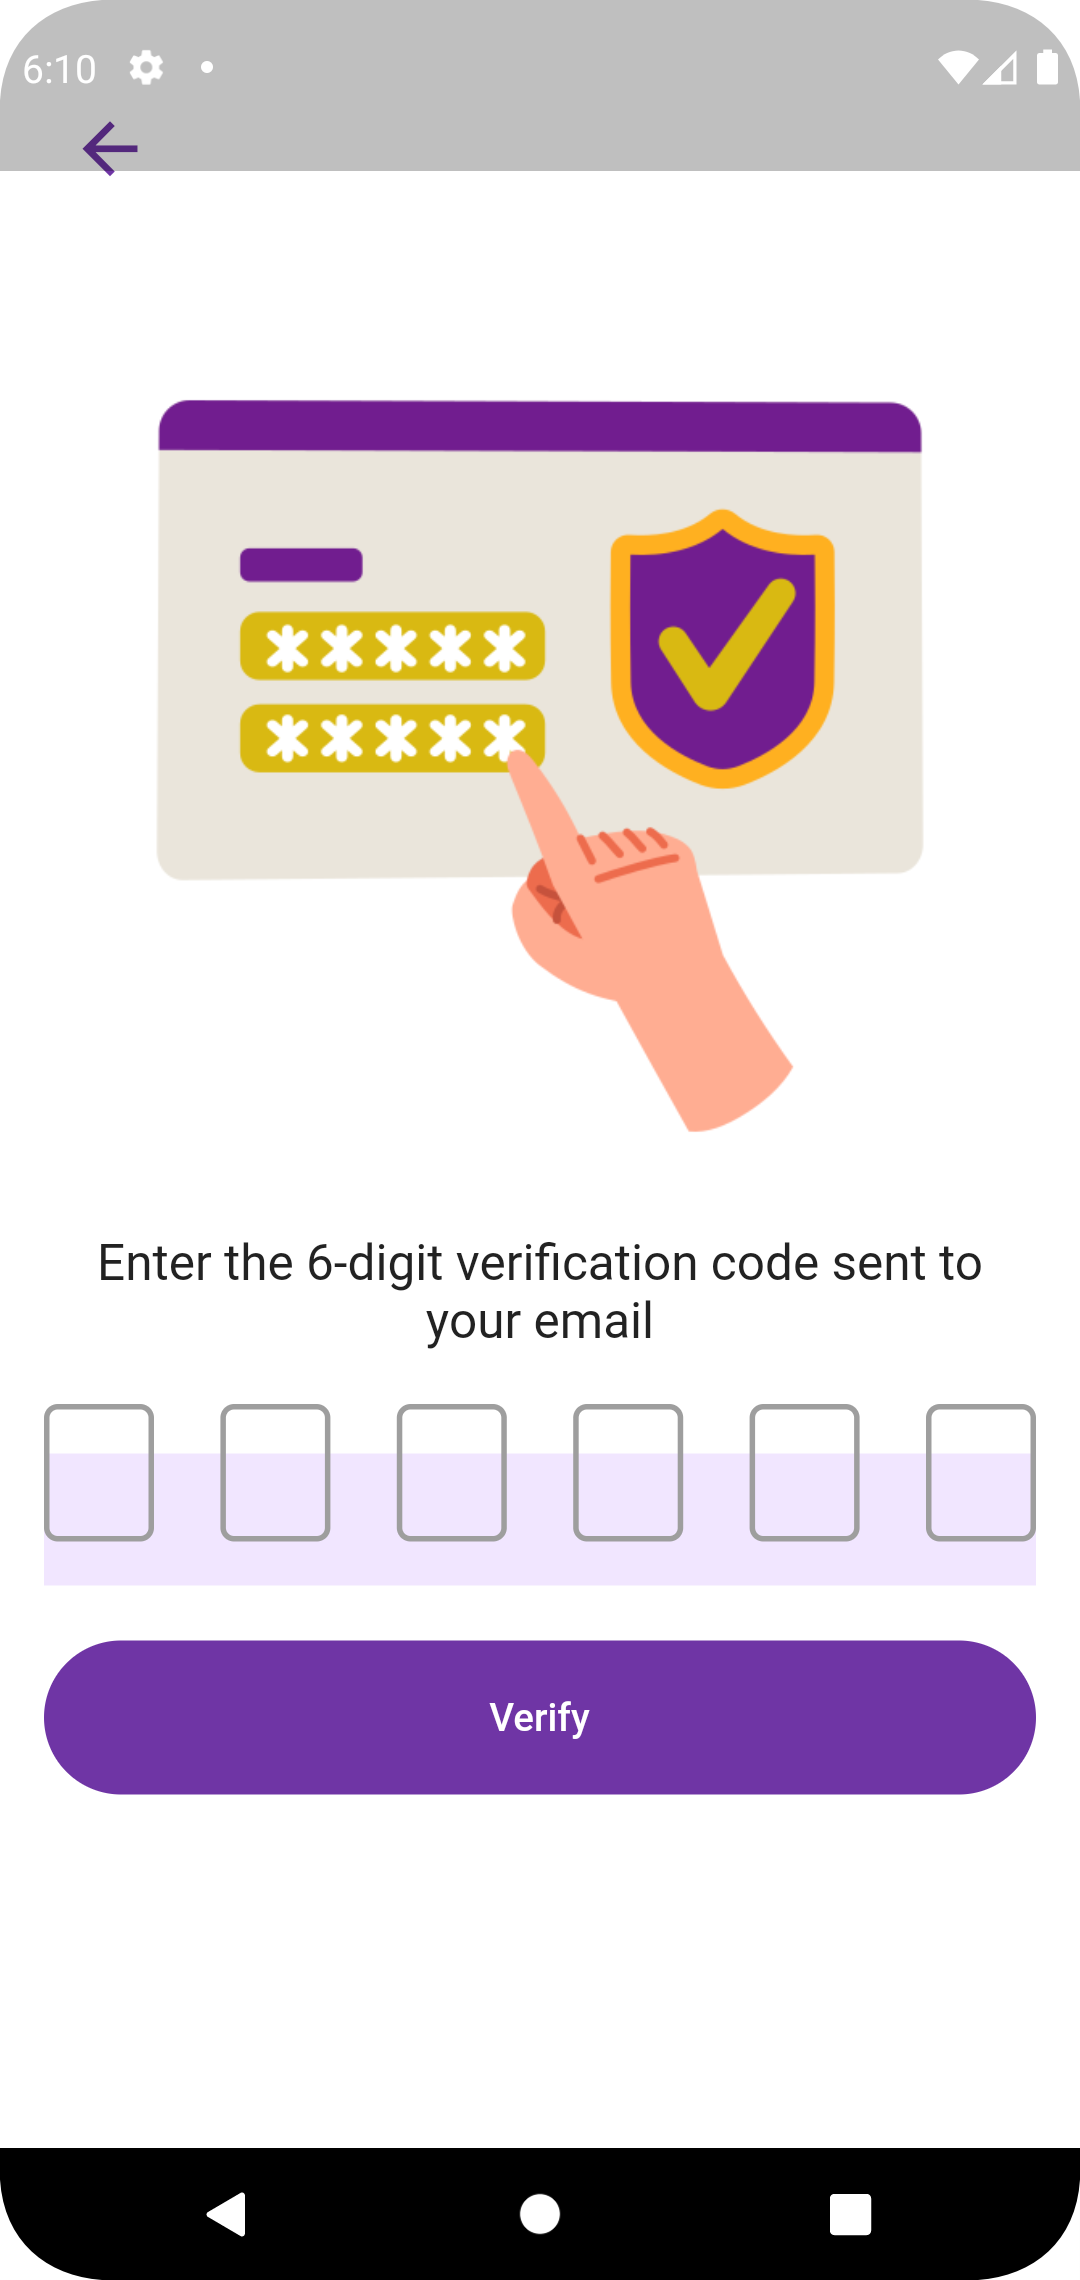
\includegraphics[height=9.2cm,width=7cm]{images/ForgetPassword2.png}
        }
        \label{fig:second}
    \end{subfigure}
    
    \vspace{-0.2cm}

    % Deuxième ligne avec une seule image centrée
    \begin{subfigure}{0.45\textwidth}
        \centering
        \setlength{\fboxsep}{5pt}%
        \setlength{\fboxrule}{0.5pt}%
        \fbox{
            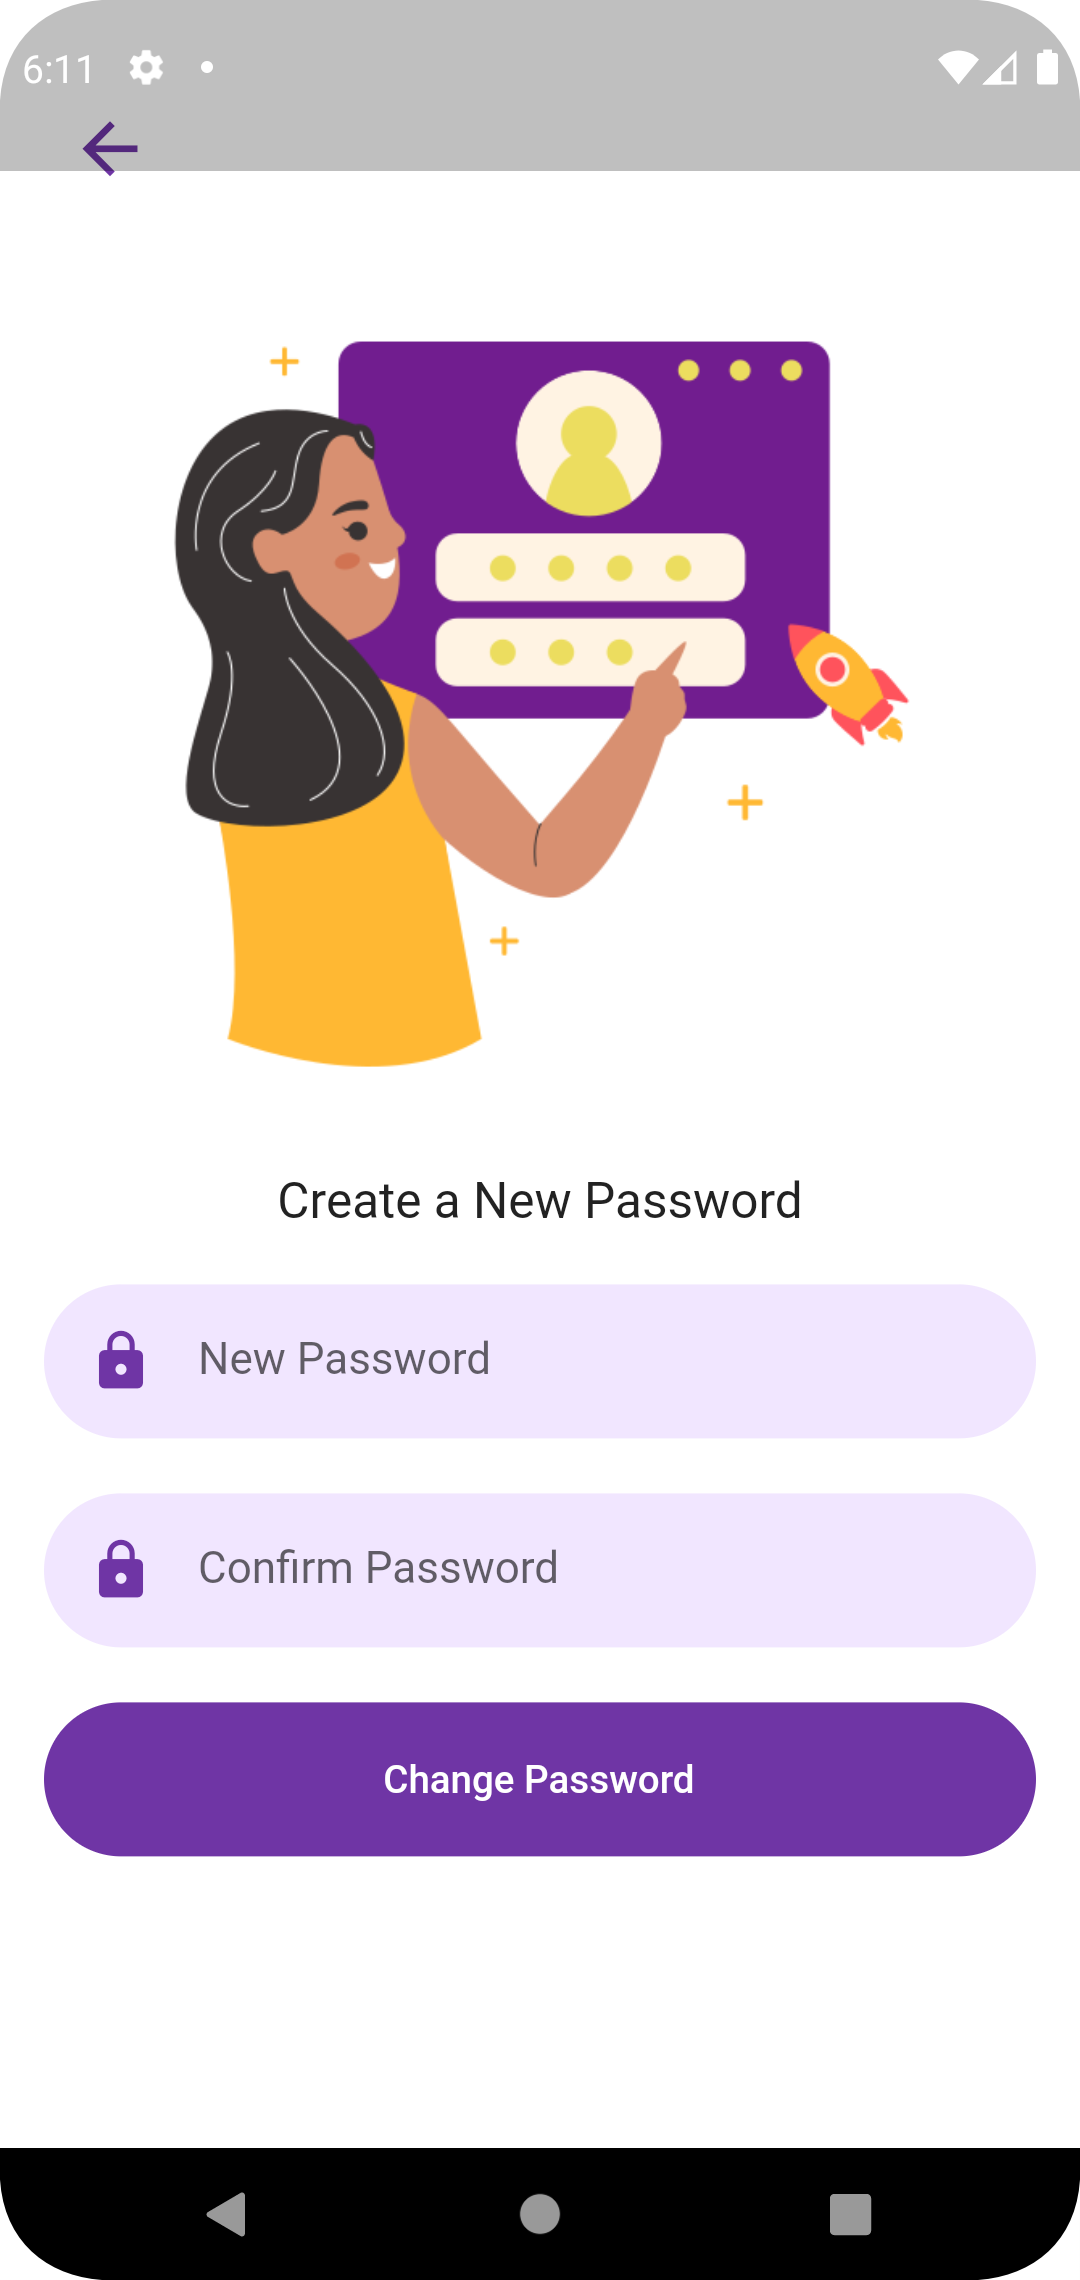
\includegraphics[height=9.2cm,width=7cm]{images/ForgetPassword3.png}
        }
        \label{fig:third}
    \end{subfigure}
    \vspace{-4mm}
    \caption{Les interfaces de la page de mot de passe oublié}
    \label{fig:three}
\end{figure}


\vspace{-4mm}
\subsection{Page Profile}
\vspace{-4mm}
La page de profil utilisateur permet aux utilisateurs de visualiser et de modifier leurs informations personnelles, ainsi que de consulter les publications qu'ils ont créées et les images qu'ils ont partagées.
\begin{figure}[H]
    \centering

    % Première ligne avec deux images côte à côte
    \begin{subfigure}{0.45\textwidth}
        \centering
        \setlength{\fboxsep}{5pt}%
        \setlength{\fboxrule}{0.5pt}%
        \fbox{
            
\includegraphics[height=9.2cm,width=7cm]{images/AAAProfile.png}
        }
        \label{fig:first}
    \end{subfigure}
    \hfill
    \begin{subfigure}{0.45\textwidth}
        \centering
        \setlength{\fboxsep}{5pt}%
        \setlength{\fboxrule}{0.5pt}%
        \fbox{
            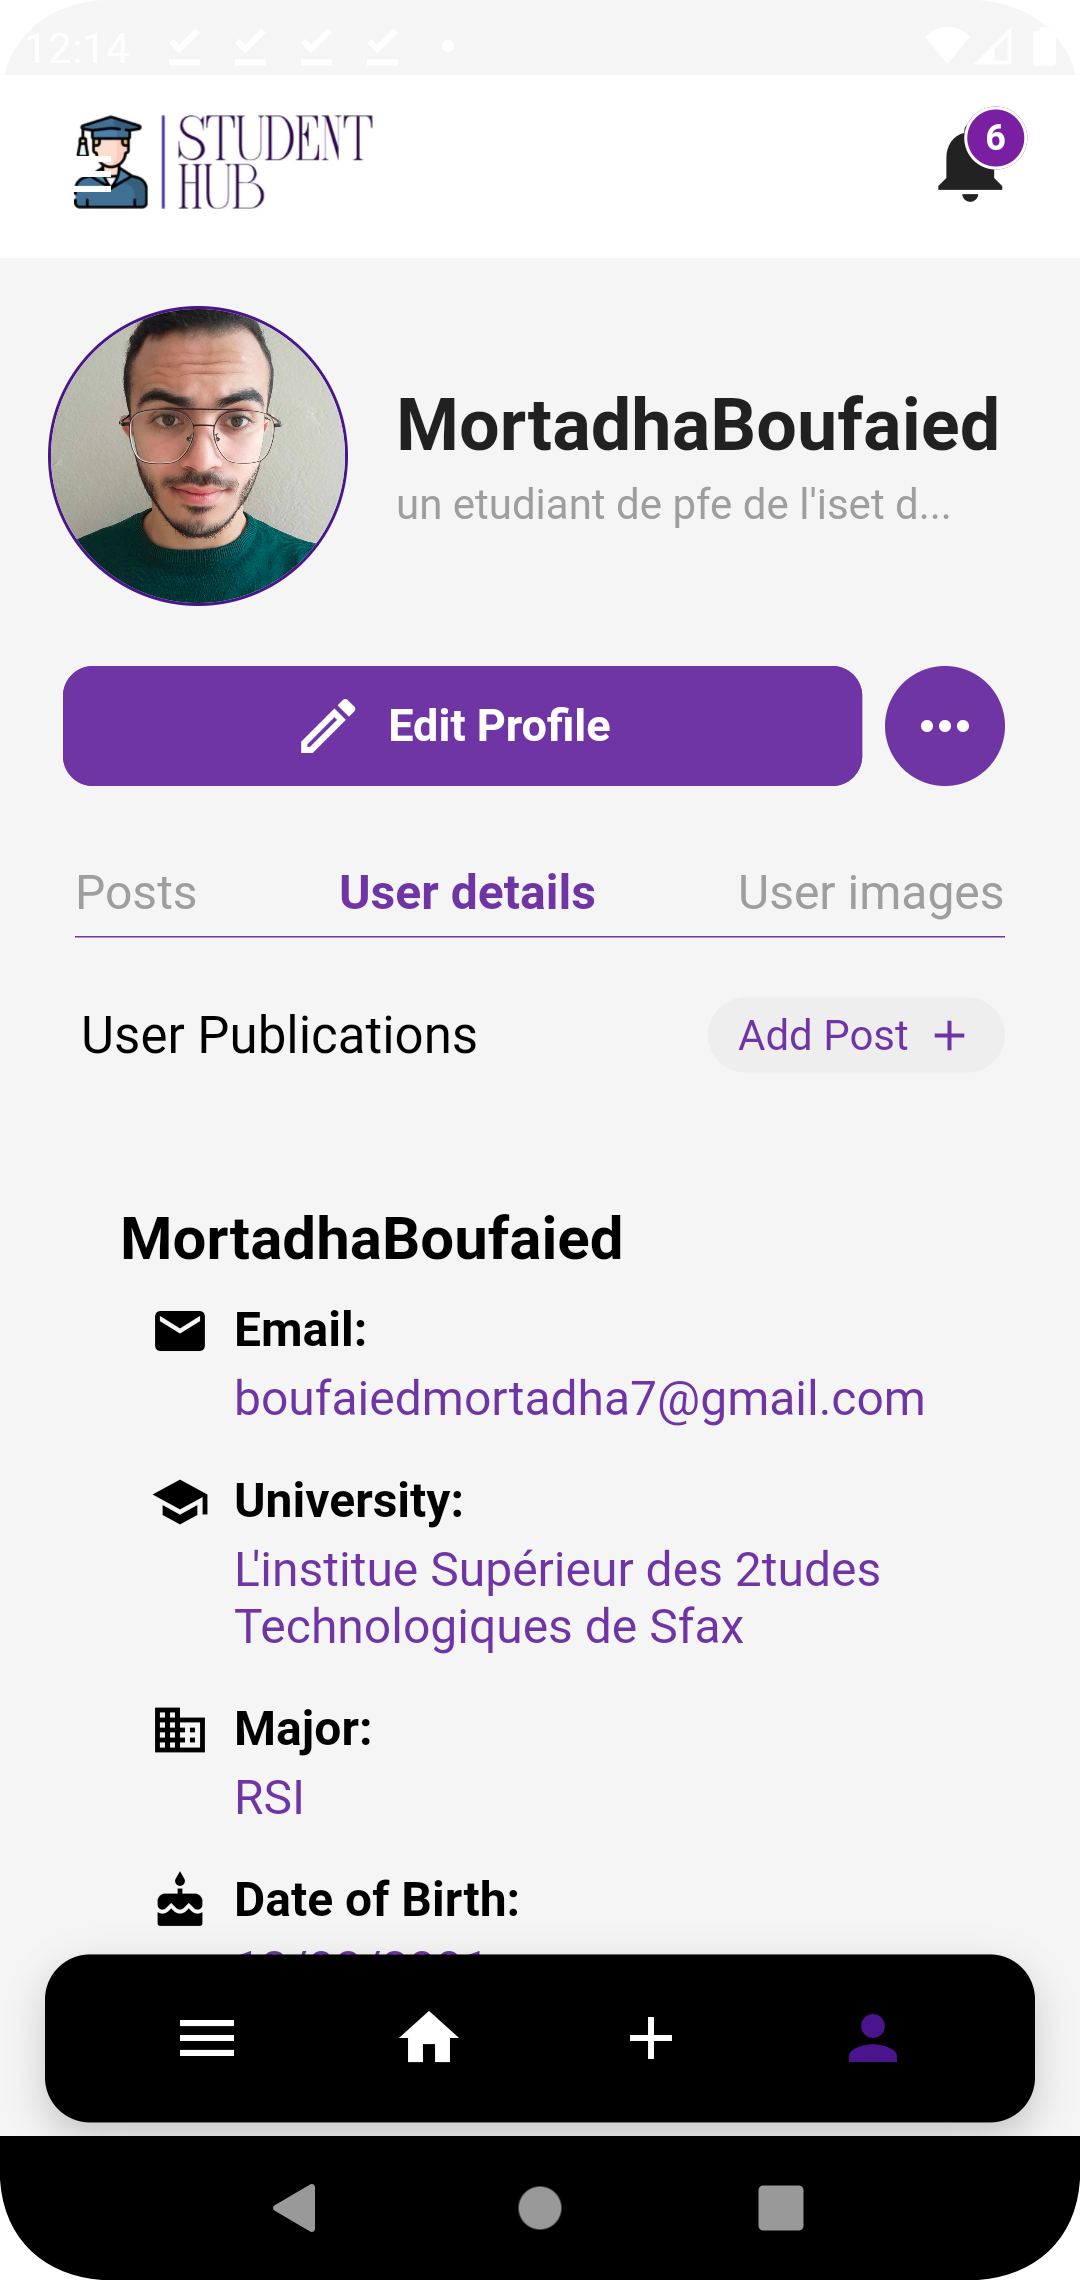
\includegraphics[height=9.2cm,width=7cm]{images/AAAUserDetails.png}
        }
        \label{fig:second}
    \end{subfigure}
    
    \vspace{-0.2cm}

    % Deuxième ligne avec une seule image centrée
    \begin{subfigure}{0.45\textwidth}
        \centering
        \setlength{\fboxsep}{5pt}%
        \setlength{\fboxrule}{0.5pt}%
        \fbox{
            
\includegraphics[height=9.2cm,width=7cm]{images/AAAUserImages.png}
        }
        \label{fig:third}
    \end{subfigure}
    \vspace{-5mm}
    \caption{Les interfaces du page profile}
    \label{fig:three}
\end{figure}

\vspace{-4mm}
\newpage
\section{Conclusion }
\vspace{-4mm}
Ce premier sprint a été essentiel pour mettre en place les fonctionnalités de base de notre système. Nous avons réussi à mettre en œuvre la création de comptes, l'authentification, la gestion des utilisateurs, ainsi que la réinitialisation des mots de passe. Ces fonctionnalités constituent la fondation de notre application, et nous permettront de fournir une expérience utilisateur fluide et sécurisée.. Nous passons maintenant vers le chapitre suivant qui est consacré au Sprint 2.

\end{sloppypar}



    \chapter{ Chapitre  5  : Sprint 2 " Gestion \centering  des Universités Endroits et des Examens"}
\begin{spacing}{1.2}
\minitoc
\thispagestyle{MyStyle}
\end{spacing}
\newpage
\begin{sloppypar} 

\section{Introduction }
\vspace{-4mm}
Le prochain sprint sera axé sur la gestion des universités, des Endroits et des examens, qui seront affichés sur l'application mobile pour tous les utilisateurs. L’objectif est de fournir à l’admin les outils nécessaires pour gérer efficacement et en toute sécurité les informations relatives aux universités, aux Endroits disponibles et aux examens.
\vspace{-9mm}
\section{Backlog du sprint}
\vspace{-4mm}
Le backlog de gestion des universités, des Endroits et des examens propose des fonctionnalités pour ajouter, modifier, supprimer et consulter ces informations dans notre application.
\vspace{-4mm}
\begin{table}[H]
\centering
\begin{tabular}{|p{11cm}|p{2cm}|p{2.5cm}|}
\hline
\textbf{ Tâches } & \textbf{ Priorité }& \textbf{Période/jour}  \\
\hline
En tant qu’un admin je peux gérer  les universités dans l’application web.  & Élevée  & 4 jours  \\
\hline
En tant qu’un admin je peux gérer les Endroits dans l’application web.   & Élevée  & 3 jours  \\
\hline
En tant qu’un admin je peux gérer les examens dans l’application web. & Élevée & 4 jours \\
\hline
En tant qu’un utilisateur je peux consulter  les universités dans l’application mobile. & Élevée  & 3 jours \\
\hline
En tant qu’un utilisateur je peux consulter  les Endroits dans l’application mobile. & Moyenne & 1 jour\\
\hline
En tant qu’un utilisateur je peux consulter  les examens dans l’application mobile. & Moyenne & 1 jour\\
\hline
\end{tabular}
\caption{Tableau de Backlog de produit Sprint 2}
\end{table}

\vspace{-1.3cm}
\section {Analyse et spécification des besoins}
\vspace{-7mm}
\subsection{Diagramme de cas d’utilisation detaillé}
\vspace{-4mm}
Afin de mieux comprendre la structure de notre système, nous avons utilisé un diagramme de cas d'utilisations qui est présenté ci-dessous.
\vspace{-4mm}
\begin{figure}[H]%
    \centering
    \setlength{\fboxsep}{5pt}%
    \setlength{\fboxrule}{0.5pt}%
    \fbox{
    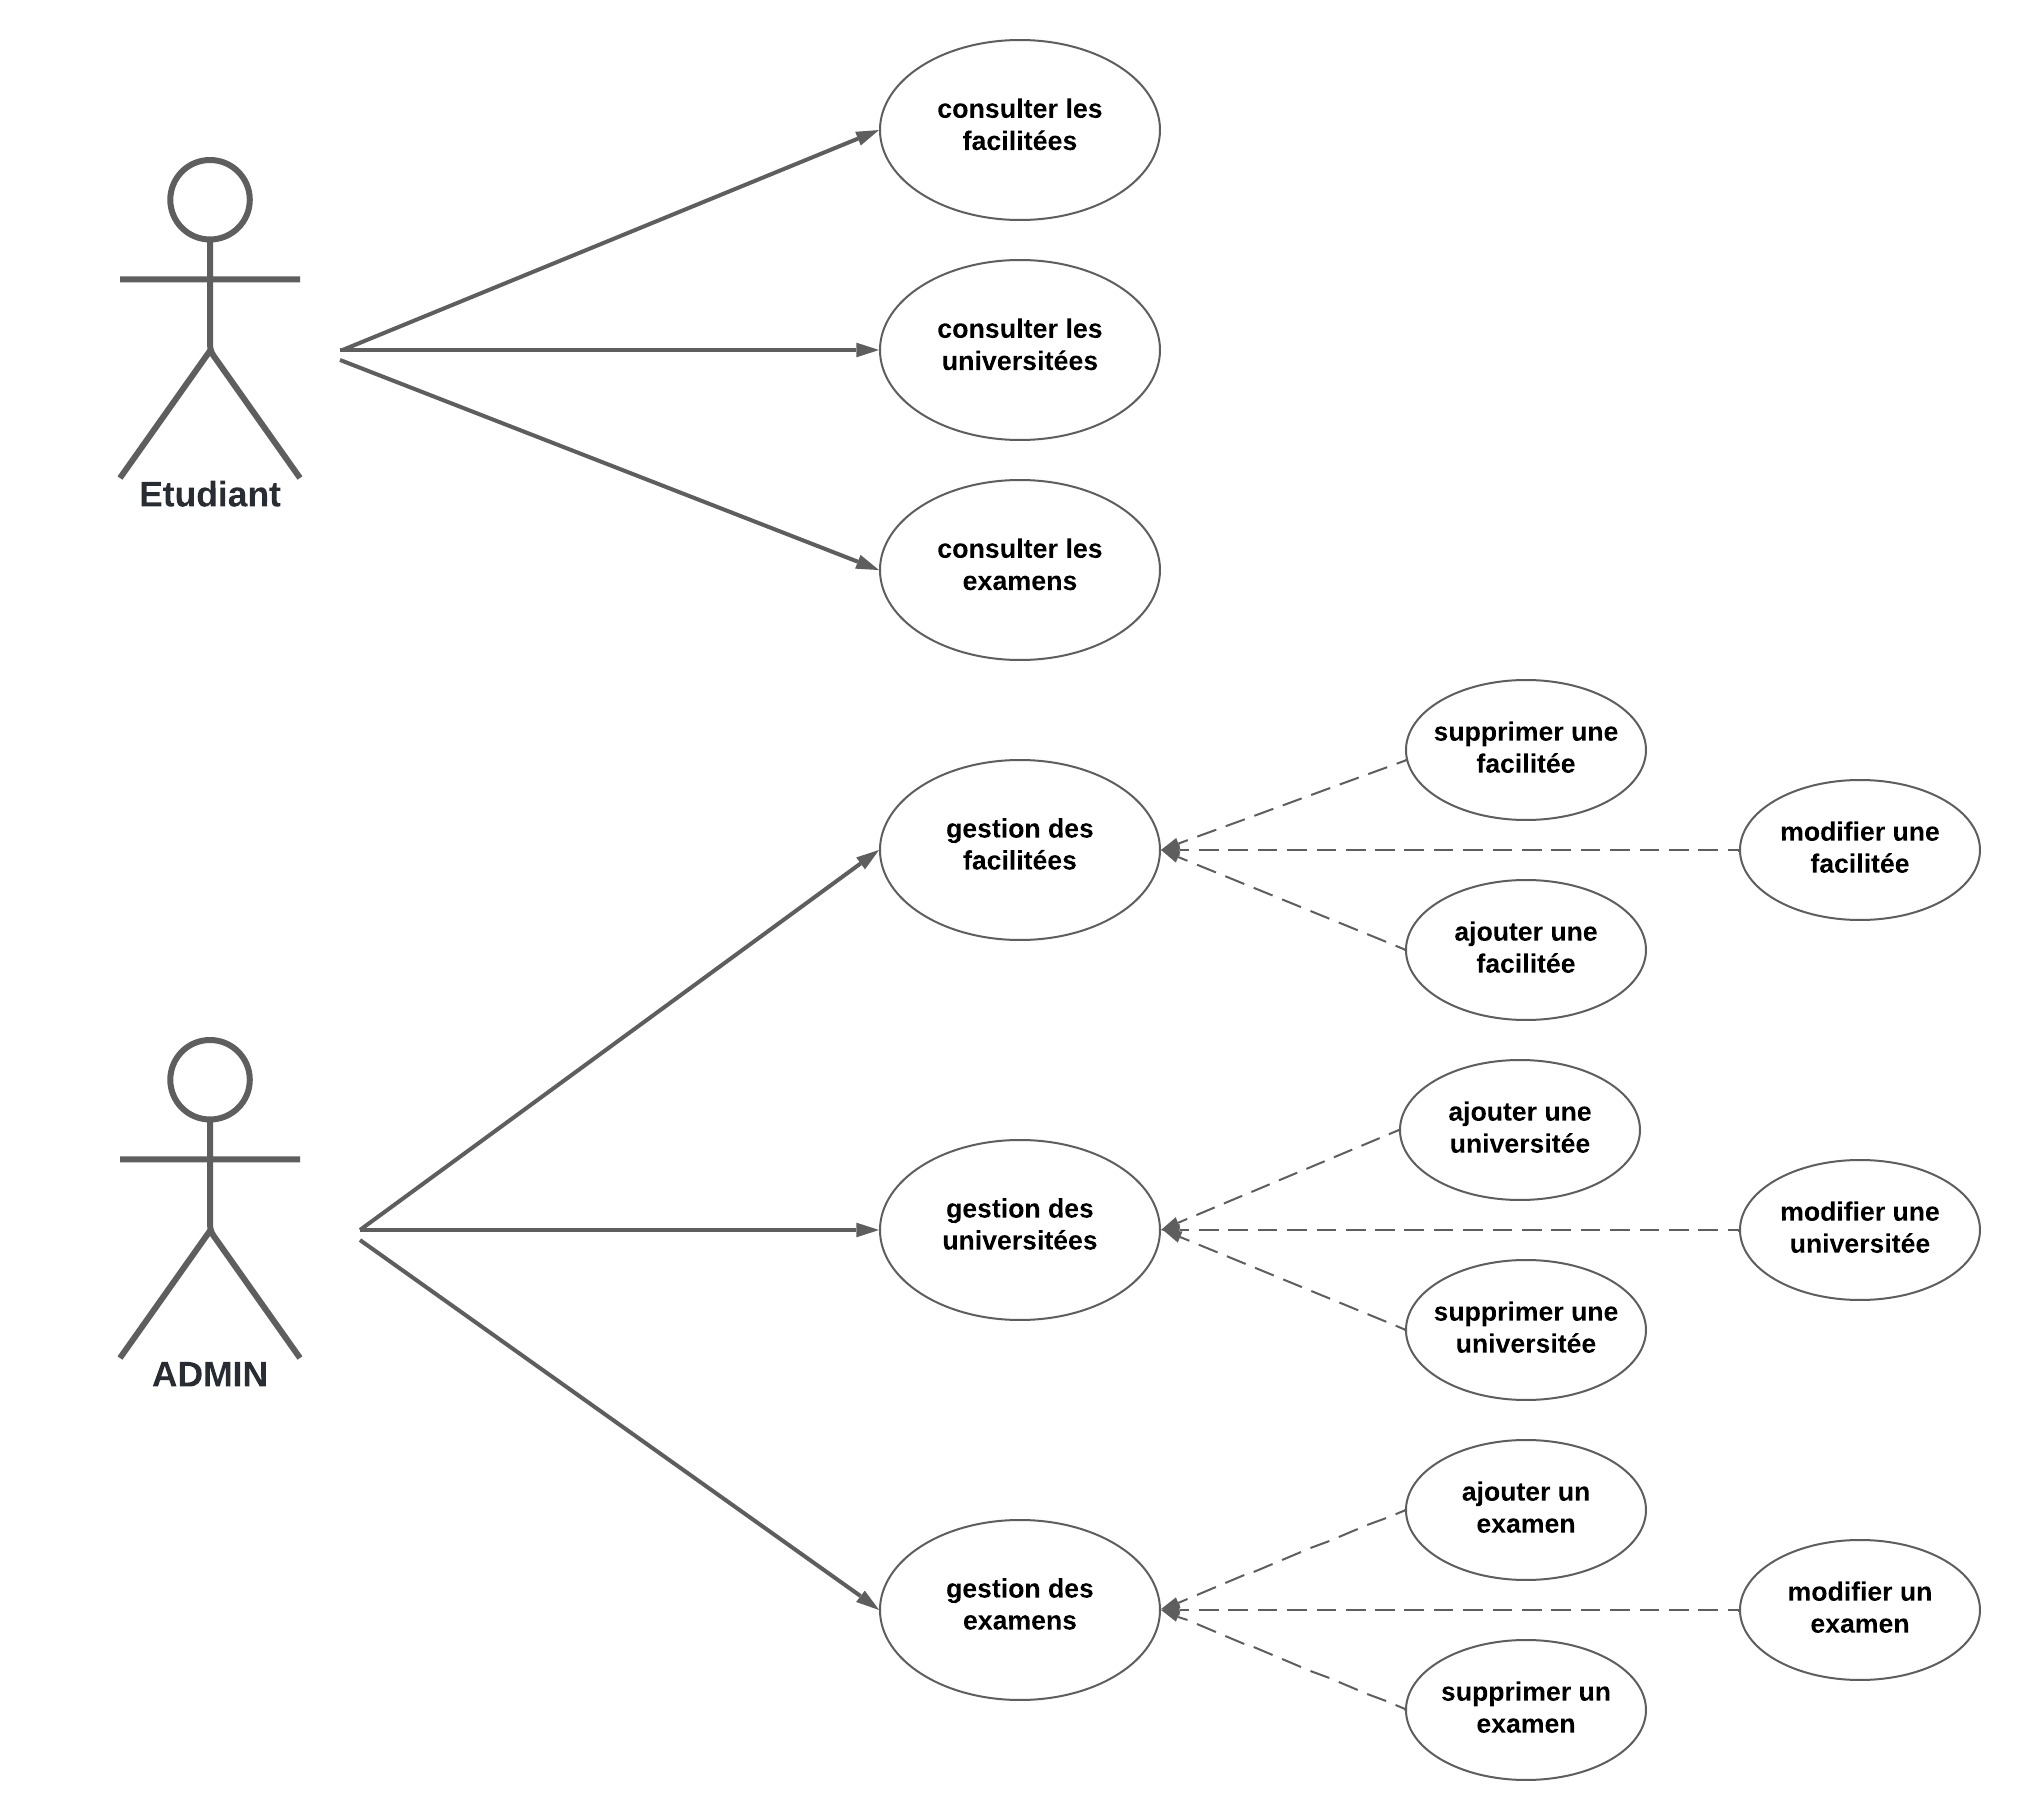
\includegraphics[height=10cm,width=15cm]{images/AAADiagrammedesCasFacUnEx.png}%
    }
    \caption{Figure du Diagramme de cas d'utilisation Sprint 2}
\end{figure}
\vspace{-1cm}
\subsection{Description textuelle du cas d’utilisation « Ajouter un endroit »}
\vspace{-3mm}
La description textuelle du cas d'utilisation "Ajouter un endroit" détaille le processus par lequel un admin peut créer un nouvel endroit sur la plateforme web de l'application, en fournissant des informations telles que le nom de l'endroit, sa localisation, sa description, etc.

\begin{table}[h]
\centering
\begin{tabular}{|p{3cm}|p{12cm}|}
\hline
\textbf{Cas d'utilisation } & Ajouter un endroit  \\
\hline
\textbf{Acteurs} & Admin \\
\hline
\textbf{Précondition} & Admin authentifié \\
\hline
\textbf{Postcondition} & endroit  ajoutée \\
\hline
\textbf{Scénario nominal} &
\begin{enumerate}
    \item Le système affiche l’interface de gestion des données.
    \item L’admin la catégorie correspondante.
    \item L'admin saisit les inforamtions necessaires .
    \item L'admin appuit sur le bouttin <<Add>>.
    \item Le système vérifie que tous les champs sont remplis. S'ils ne le sont pas, une exception est déclenchée.
    \end{enumerate} \\
\hline
\textbf{Exception } & Champs non remplis. \\
& Le système affiche un message d’erreur informant l’utilisateur que tous les champs doivent être remplis.  \\
\hline

\end{tabular}
\caption{Description du cas d’utilisation « Ajouter un endroit »}
\end{table}

\subsection{Description textuelle du cas d’utilisation « Modifier un endroit »}
\vspace{-3mm}
La description du cas d'utilisation "Modifier un endroit" décrit comment un admin peut mettre à jour les informations d'un endroit existant sur la plateforme web de l'application. Cela inclut la modification de détails tels que le nom de l'endroit, sa localisation, sa description, etc.
\begin{table}[h]
\centering
\begin{tabular}{|p{3cm}|p{12cm}|}
\hline
\textbf{Cas d'utilisation } & Modifier un endroit  \\
\hline
\textbf{Acteurs} & Admin \\
\hline
\textbf{Précondition} & Admin authentifié \\
\hline
\textbf{Postcondition} & endroit  modifié \\
\hline
\textbf{Scénario nominal} &
\begin{enumerate}
    \item Le système affiche l’interface de gestion des données.
    \item L’admin la catégorie correspondante.
    \item L'admin modifie les inforamtions  .
    \item L'admin appuit sur le bouttin <<Edit>>.
    \item Le système vérifie que tous les champs sont remplis. S'ils ne le sont pas, une exception est déclenchée.
    \end{enumerate} \\
\hline
\textbf{Exception } & Champs non remplis. \\
& Le système affiche un message d’erreur informant l’utilisateur que tous les champs doivent être remplis.  \\
\hline

\end{tabular}
\caption{Description du cas d’utilisation « Modifier un endroit »}
\end{table}
\vspace{-1cm}
\subsection{Description textuelle du cas d’utilisation « Supprimer un endroit »}
\vspace{-4mm}
La description du cas d'utilisation "Supprimer un endroit" décrit le processus par lequel un administrateur peut retirer un endroit de la plateforme web de l'application. Cela implique de sélectionner l'endroit à supprimer, puis de confirmer cette action. Une fois supprimé, l'endroit ne sera plus visible pour les utilisateurs de l'application.


\begin{table}[h]
\centering
\begin{tabular}{|p{3cm}|p{12cm}|}
\hline
\textbf{Cas d'utilisation } &  supprimer un endroit  \\
\hline
\textbf{Acteurs} & Admin \\
\hline
\textbf{Précondition} & Admin authentifié \\
\hline
\textbf{Postcondition} & endroit  supprimé \\
\hline
\textbf{Scénario nominal} &
\begin{enumerate}
    \item Le système affiche l’interface de gestion des données.
    \item L’admin la catégorie correspondante.
    \item L'admin modifie les inforamtions  .
    \item L'admin appuit sur le bouttin <<Delete>>.
    \end{enumerate} \\
\hline
\end{tabular}
\caption{Description du cas d’utilisation «  Supprimer un endroit  »}
\end{table}
\vspace{-1cm}
\section{Diagramme de séquence }
\vspace{-4mm}
Les diagrammes de séquence décrivent de manière séquentielle les interactions entre l'utilisateur et le système lors de la gestion des endroits.
\vspace{-7mm}
\subsection{Diagramme de séquence « Ajouter un Endroit »}
\vspace{-4mm}
Le diagramme présente le processus d'ajout d'un nouvel endroit par l'administrateur sur la partie web de notre application.
\begin{figure}[H]%
    \center%
    \setlength{\fboxsep}{5pt}%
    \setlength{\fboxrule}{0.5pt}%
    \fbox{
    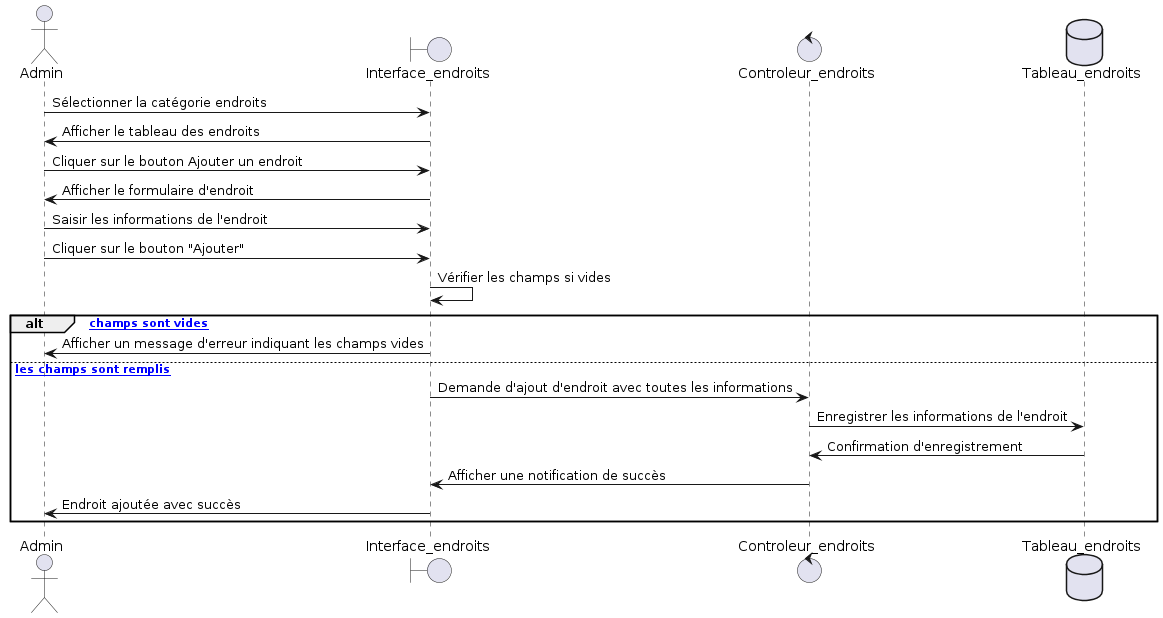
\includegraphics[height=13.5cm,width=15cm]{images/ffffajouterandroit.png}%
    }
    \caption{Figure du Diagramme de Séquence «Ajouter un Endorit» }
\end{figure}
\vspace{-1.2cm}
\subsection{Diagramme de séquence « Modifier un Endroit »}
\vspace{-4MM}
Le diagramme illustre le processus de modification d'un emplacement par l'admin sur la partie web de notre application.
\begin{figure}[H]%
    \center%
    \setlength{\fboxsep}{5pt}%
    \setlength{\fboxrule}{0.5pt}%
    \fbox{
    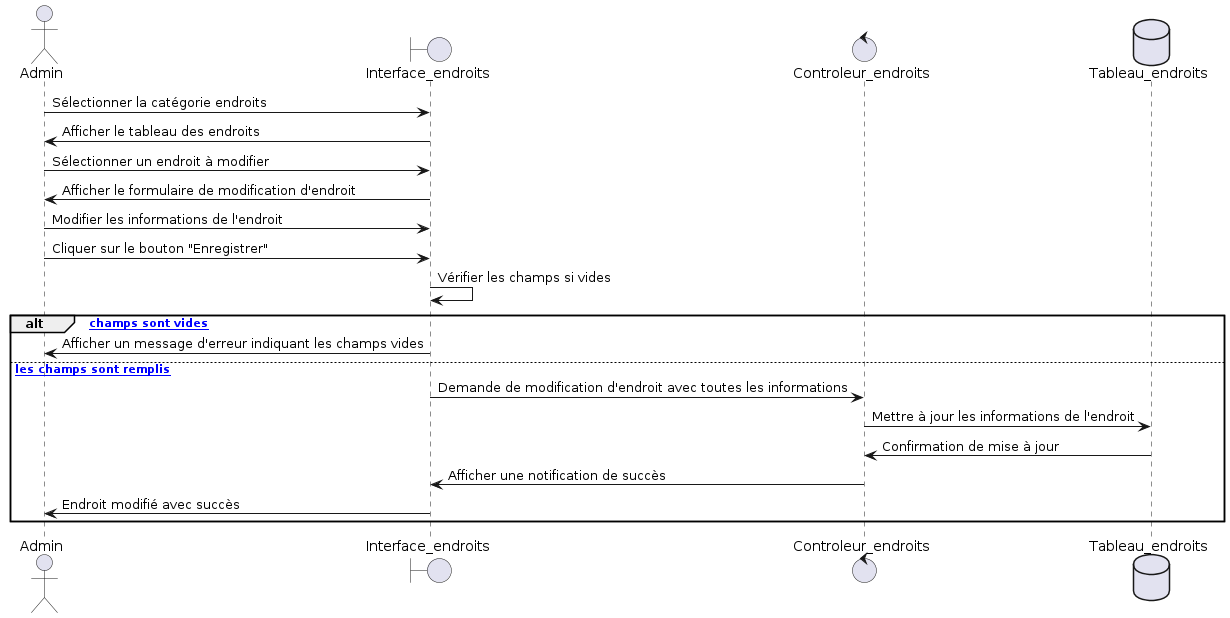
\includegraphics[height=9cm,width=15cm]{images/ffffeditendroit.png}%
    }
    \caption{Figure du Diagramme de Séquence «Modifier un Endroit» }
\end{figure}
\vspace{-1.2cm}
\subsection{Diagramme de séquence « Supprimer un Endroit »}
\vspace{-4mm}
Le diagramme représente l'action effectuée par l'admin sur la partie web de notre application pour supprimer un emplacement spécifique.

\begin{figure}[H]%
    \center%
    \setlength{\fboxsep}{5pt}%
    \setlength{\fboxrule}{0.5pt}%
    \fbox{
    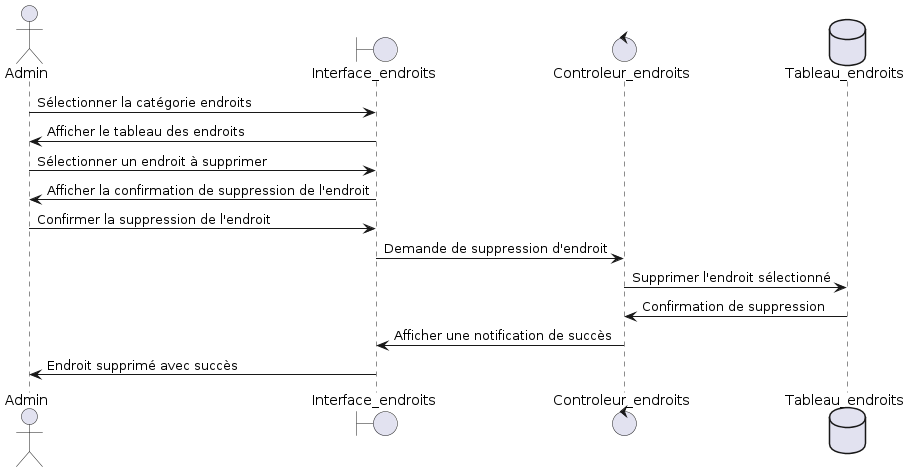
\includegraphics[height=9cm,width=15cm]{images/ffffsuppendroiy.png}%
    }
    \caption{Figure du Diagramme de Séquence «Supprimer un Endorit» }
\end{figure}
\newpage

\section{Diagramme de classes }
\vspace{-4mm}
Le diagramme de classes ci-dessus représente la gestion des universités, des facultés et des examens dans notre système. Chaque entité est modélisée par une classe correspondante, décrivant ses attributs et méthodes associées. Cette conception permet de visualiser clairement la structure des données et les relations entre les différentes entités, facilitant ainsi le développement et la maintenance du système.
\begin{figure}[H]%
    \center%
    \setlength{\fboxsep}{5pt}%
    \setlength{\fboxrule}{0.5pt}%
    \fbox{
    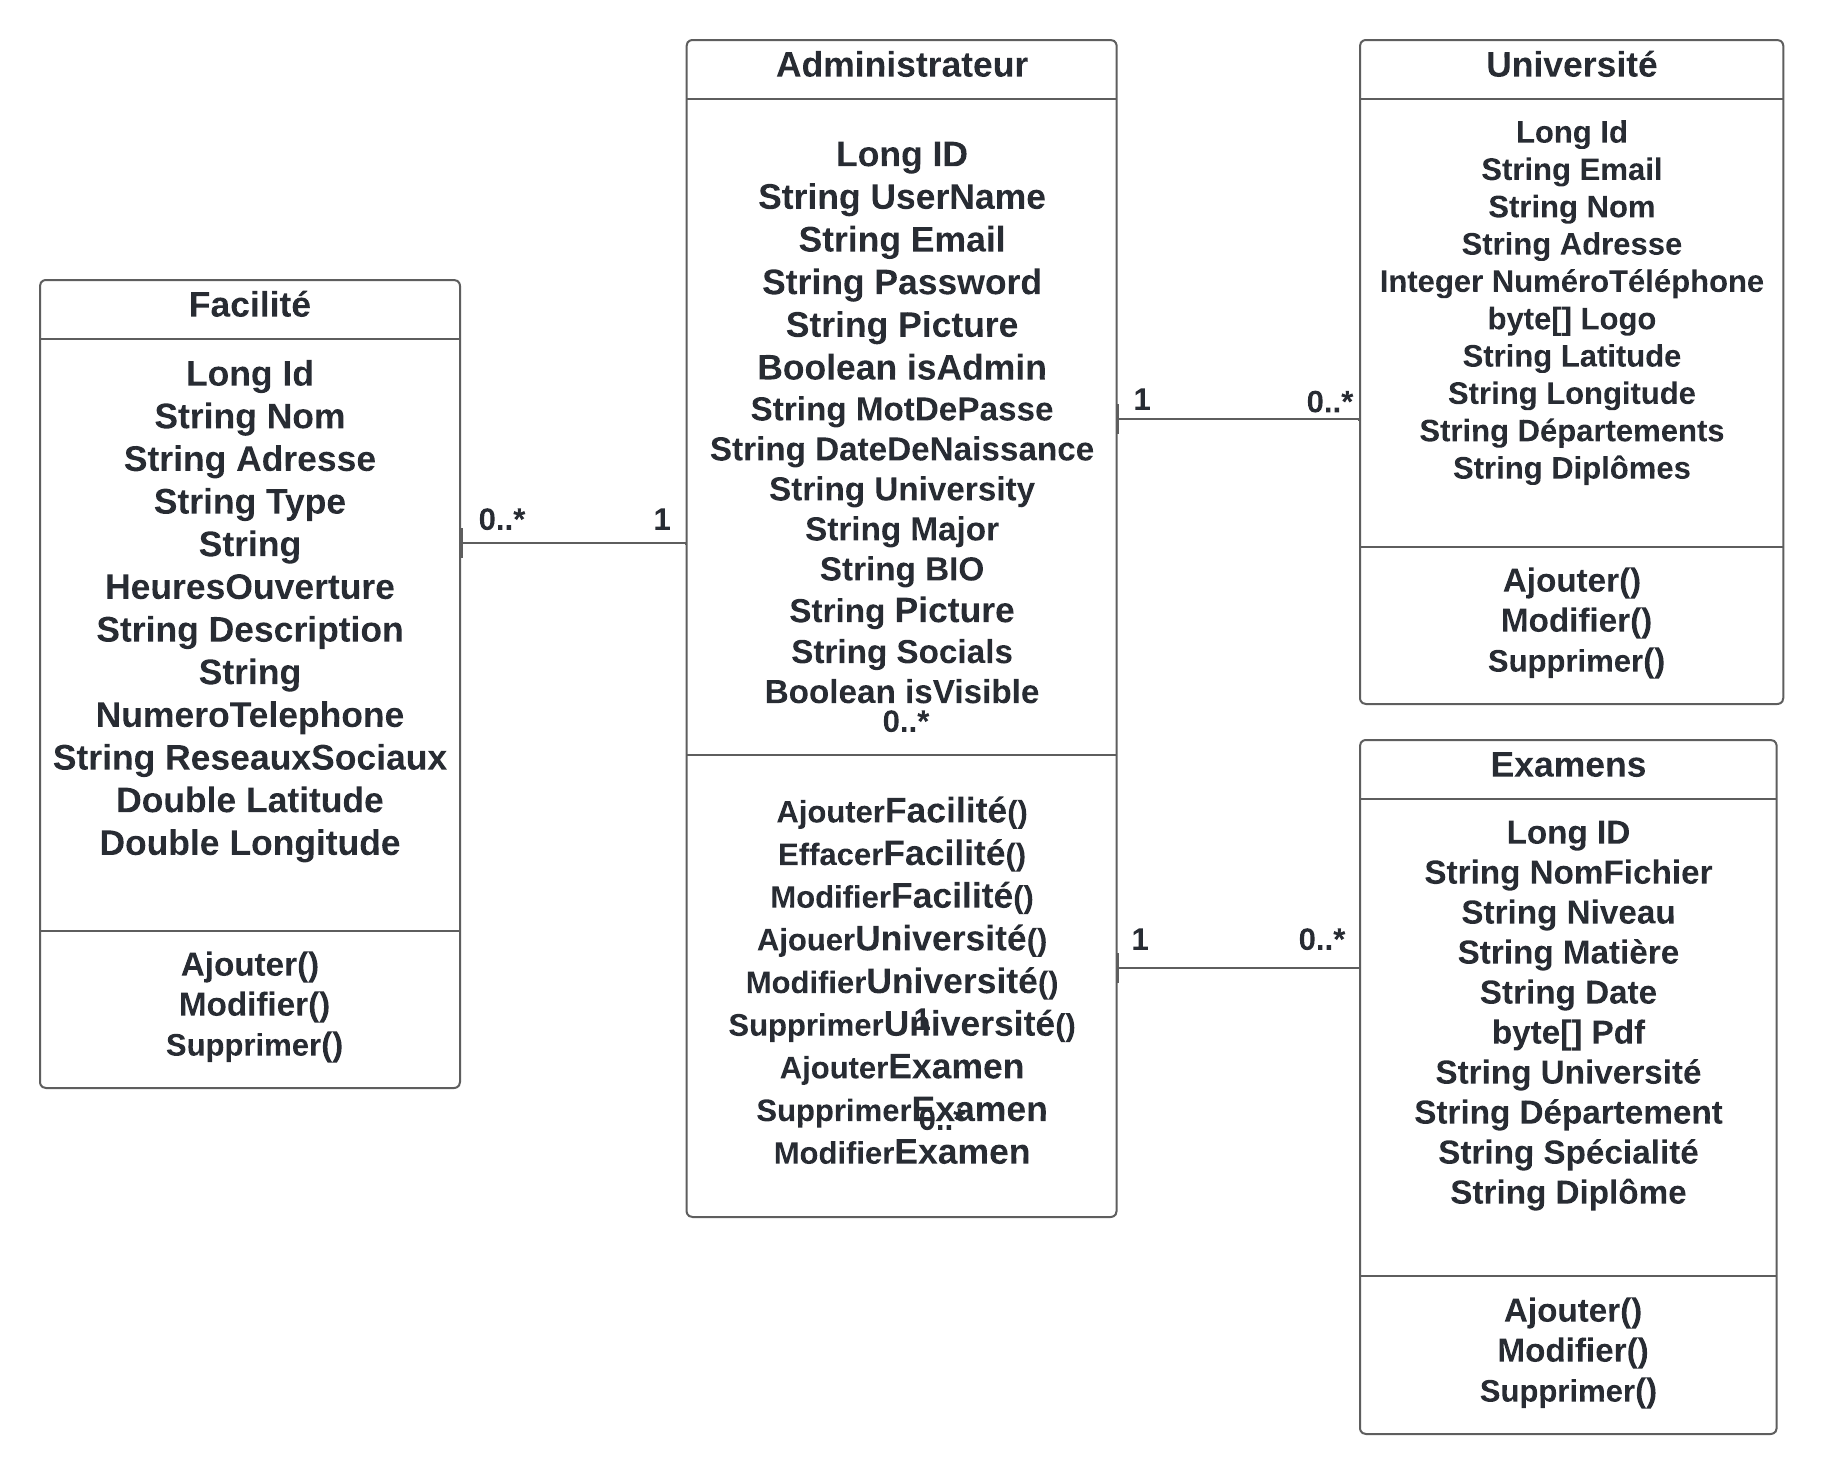
\includegraphics[height=17cm,width=15cm]{images/AAADiagramClassesUniExFac.png}%
    }
    \caption{Figure du Diagramme de classes de Sprint 2 }
\end{figure}

\section{Réalisation}
\vspace{-4mm}
La partie de réalisation représente la dernière phase du cycle de développement d’un sprint. Elle permet de présenter les résultats obtenus lors de l’étape de développement afin d’assurer et de garantir une version de qualité. Nous allons montrer cela par des captures d’écrans des fonctionnalités ayant été développées.
\vspace{-9Mm}
\subsection{Consultation de la liste des universités}
\vspace{-4mm}
L’interface d’ajout d'une université, c’est le premièr formulaire a remplir par l'admin .
\begin{figure}[H]%
    \center%
    \setlength{\fboxsep}{5pt}%
    \setlength{\fboxrule}{0.5pt}%
    \fbox{
    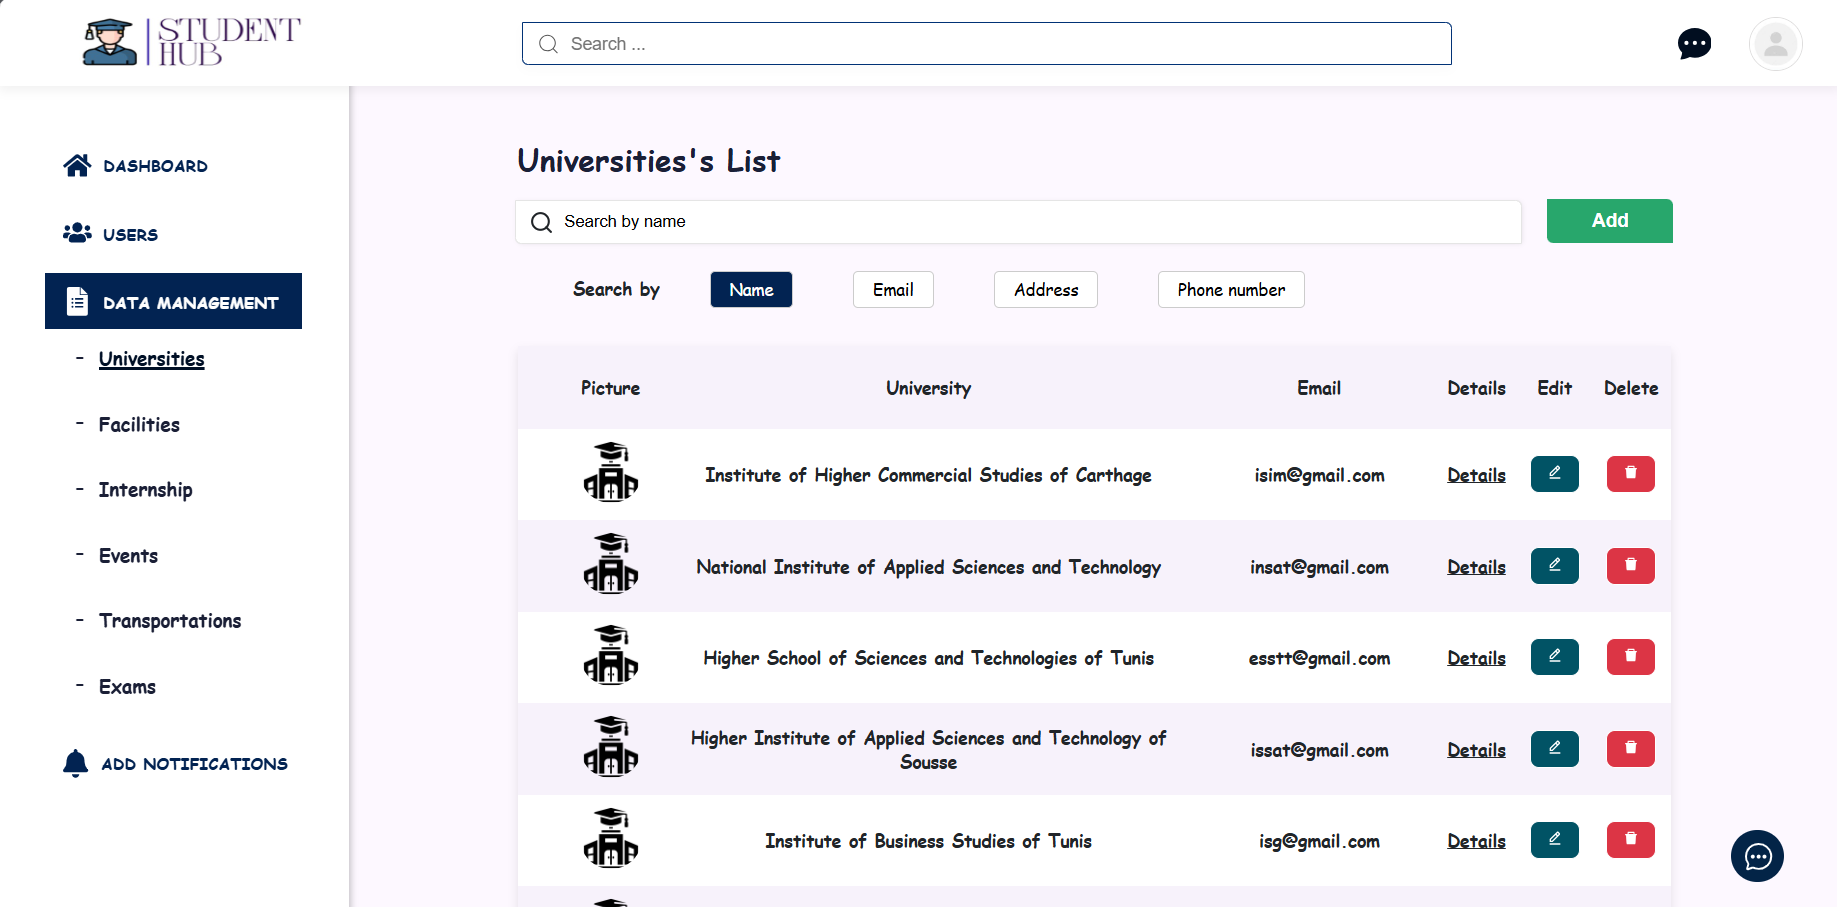
\includegraphics[height=14cm,width=16cm]{images/AAAUniversitiesPage.png}%
    }
    \caption{Interface Tableau des universités }
\end{figure}
\vspace{-1.2cm}
\subsection{Ajout d'une univesité}
\vspace{-4mm}
L’interface d’ajout d'une université, c’est le premièr formulaire a remplir par l'admin .
\vspace{-4mm}

\begin{figure}[htbp]
    \centering
    \setlength{\fboxsep}{5pt}%
    \setlength{\fboxrule}{0.5pt}%
    \fbox{
        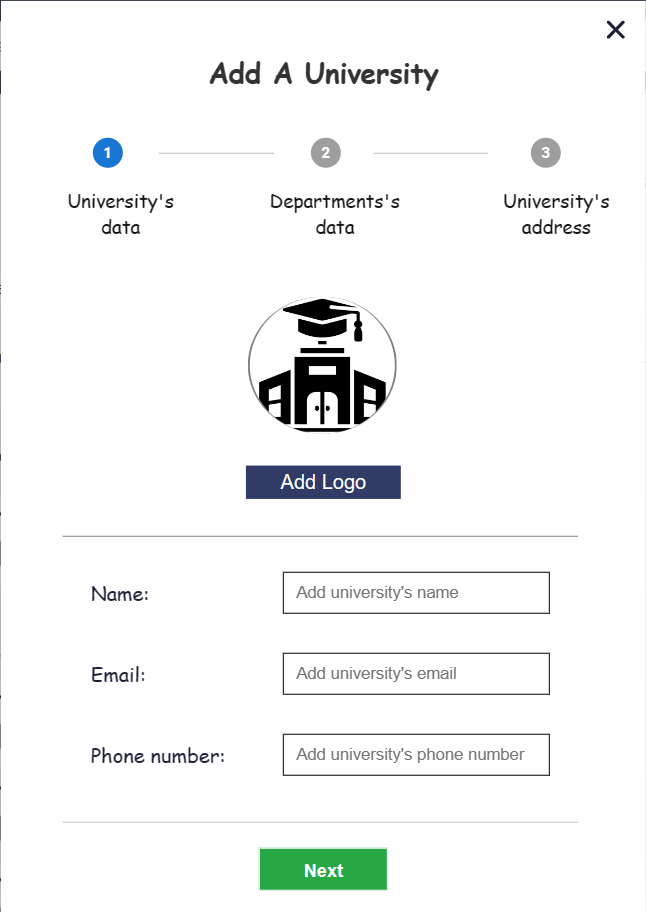
\includegraphics[height=7cm,width=12cm]{images/XAddUniversity1.png}
    }
    \label{fig:image1}
\end{figure}

\begin{figure}[htbp]
    \centering
    \setlength{\fboxsep}{5pt}%
    \setlength{\fboxrule}{0.5pt}%
    \fbox{
        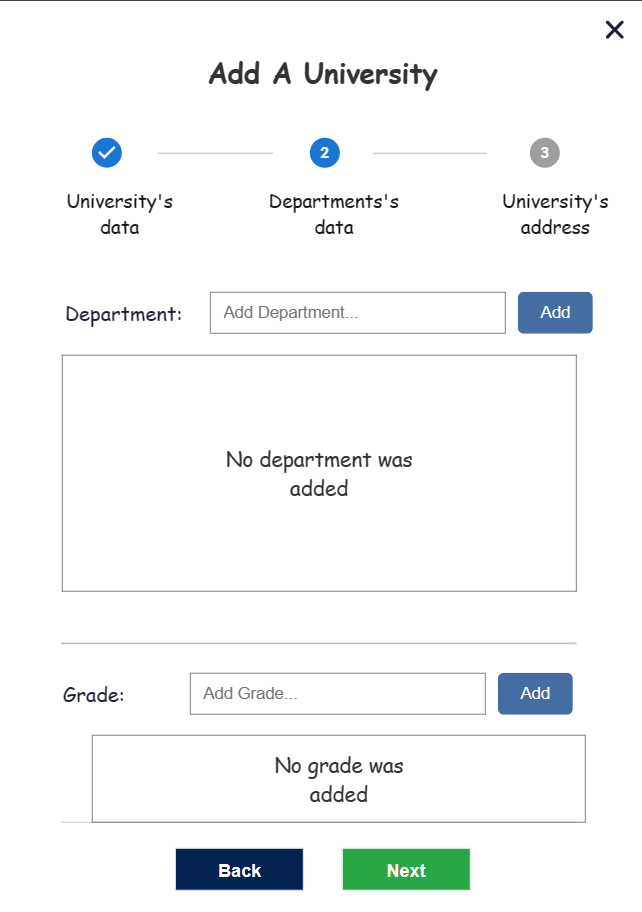
\includegraphics[height=7cm,width=12cm]{images/XAddUniversity2.png}
    }
    \label{fig:image2}
\end{figure}

\begin{figure}[htbp]
    \centering
    \setlength{\fboxsep}{5pt}%
    \setlength{\fboxrule}{0.5pt}%
    \fbox{
        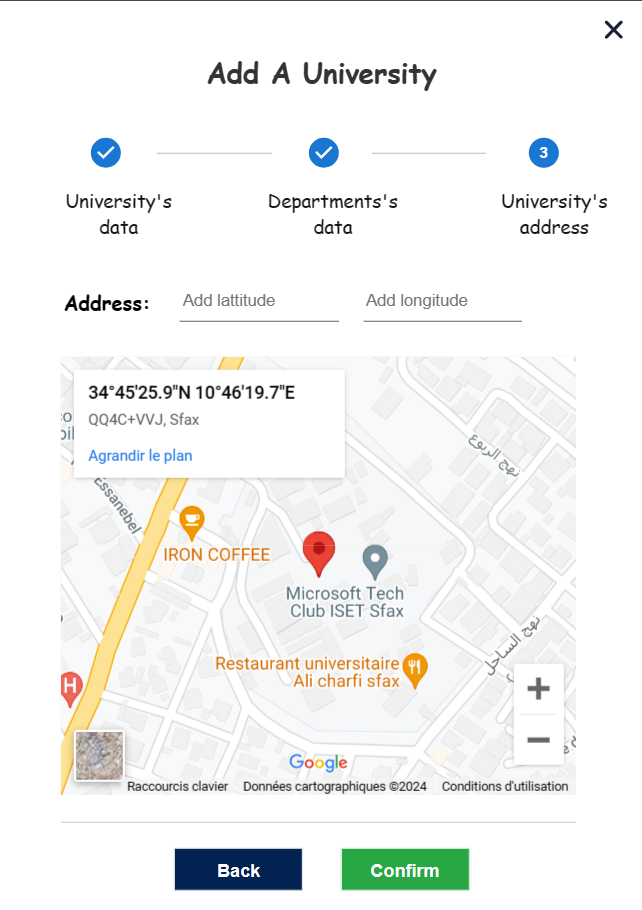
\includegraphics[height=7cm,width=12cm]{images/XAddUniversity3.png}
    }
    \caption{Interfaces d'ajout des universités}
    \label{fig:image3}
\end{figure}










\subsection{Modifier un endroit }
\vspace{-4mm}
interface de modification d'un endroit  par l'admin dans la base de données.
\vspace{-4mm}
\begin{figure}[H]%
    \center%
    \setlength{\fboxsep}{5pt}%
    \setlength{\fboxrule}{0.5pt}%
    \fbox{
    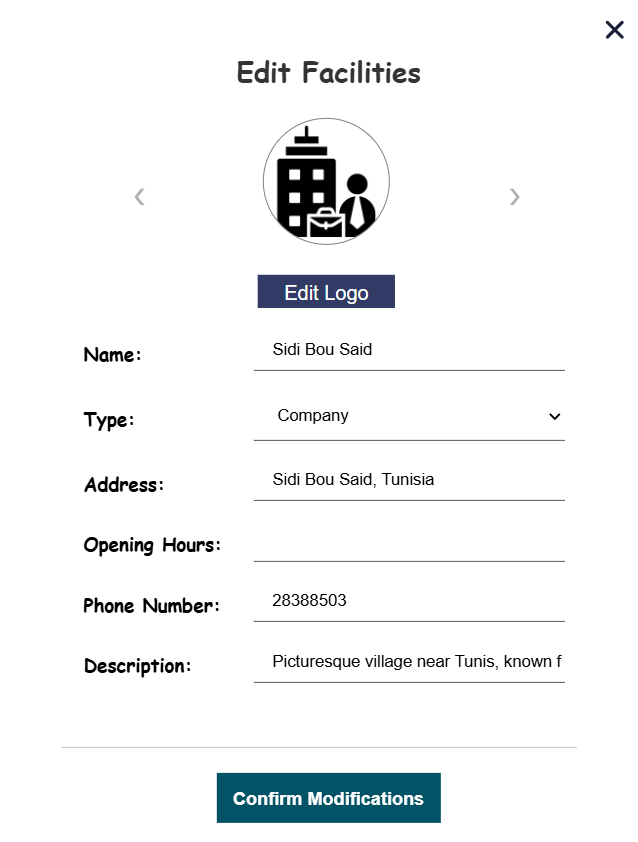
\includegraphics[height=8cm,width=12cm]{images/AAAEditFacility.png}%
    }
    \caption{Interface de modification d'un endroit  }
\end{figure}
\vspace{-1.2cm}
\subsection{Détails d'un examen}
\vspace{-4mm}
L'ad a la possibilité de consulter les détails des examens. Il peut afficher les examens directement sur le serveur sans les télécharger. De plus, l'admin peut également télécharger les examens sur son appareil si nécessaire.
\vspace{-2mm}
\begin{figure}[H]%
    \center%
    \setlength{\fboxsep}{5pt}%
    \setlength{\fboxrule}{0.5pt}%
    \fbox{
    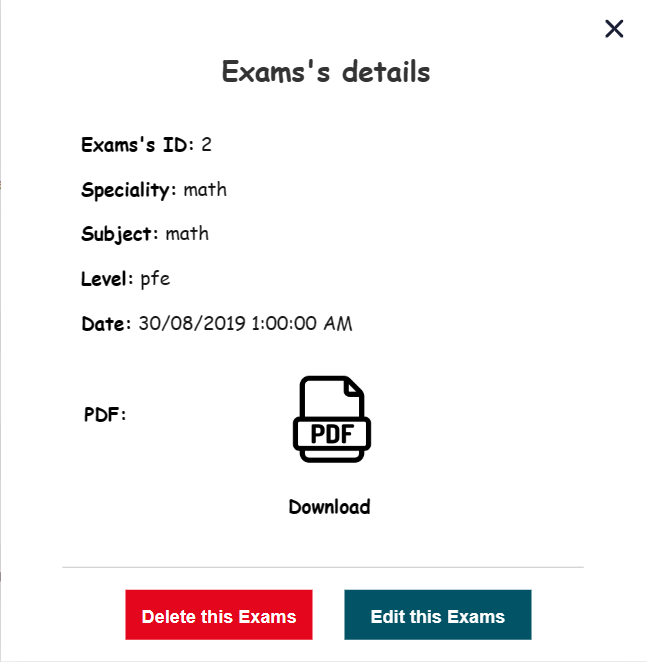
\includegraphics[height=8cm,width=12cm]{images/XExamsDetails.png}%
    }
    \caption{Interface de details d'un examen }
\end{figure}
\vspace{-4mm}
\newpage

\subsection{Détails Endroit dans l'application Mobile}
\vspace{-6mm}
L'interface "Détails Endroit" de l'appli mobile présente de façon détaillée les informations spécifiques d'un lieu, permettant aux utilisateurs d'accéder à toutes les données pertinentes.
\vspace{-4mm}
\begin{figure}[H]%
    \center%
    \setlength{\fboxsep}{5pt}%
    \setlength{\fboxrule}{0.5pt}%
    \fbox{
    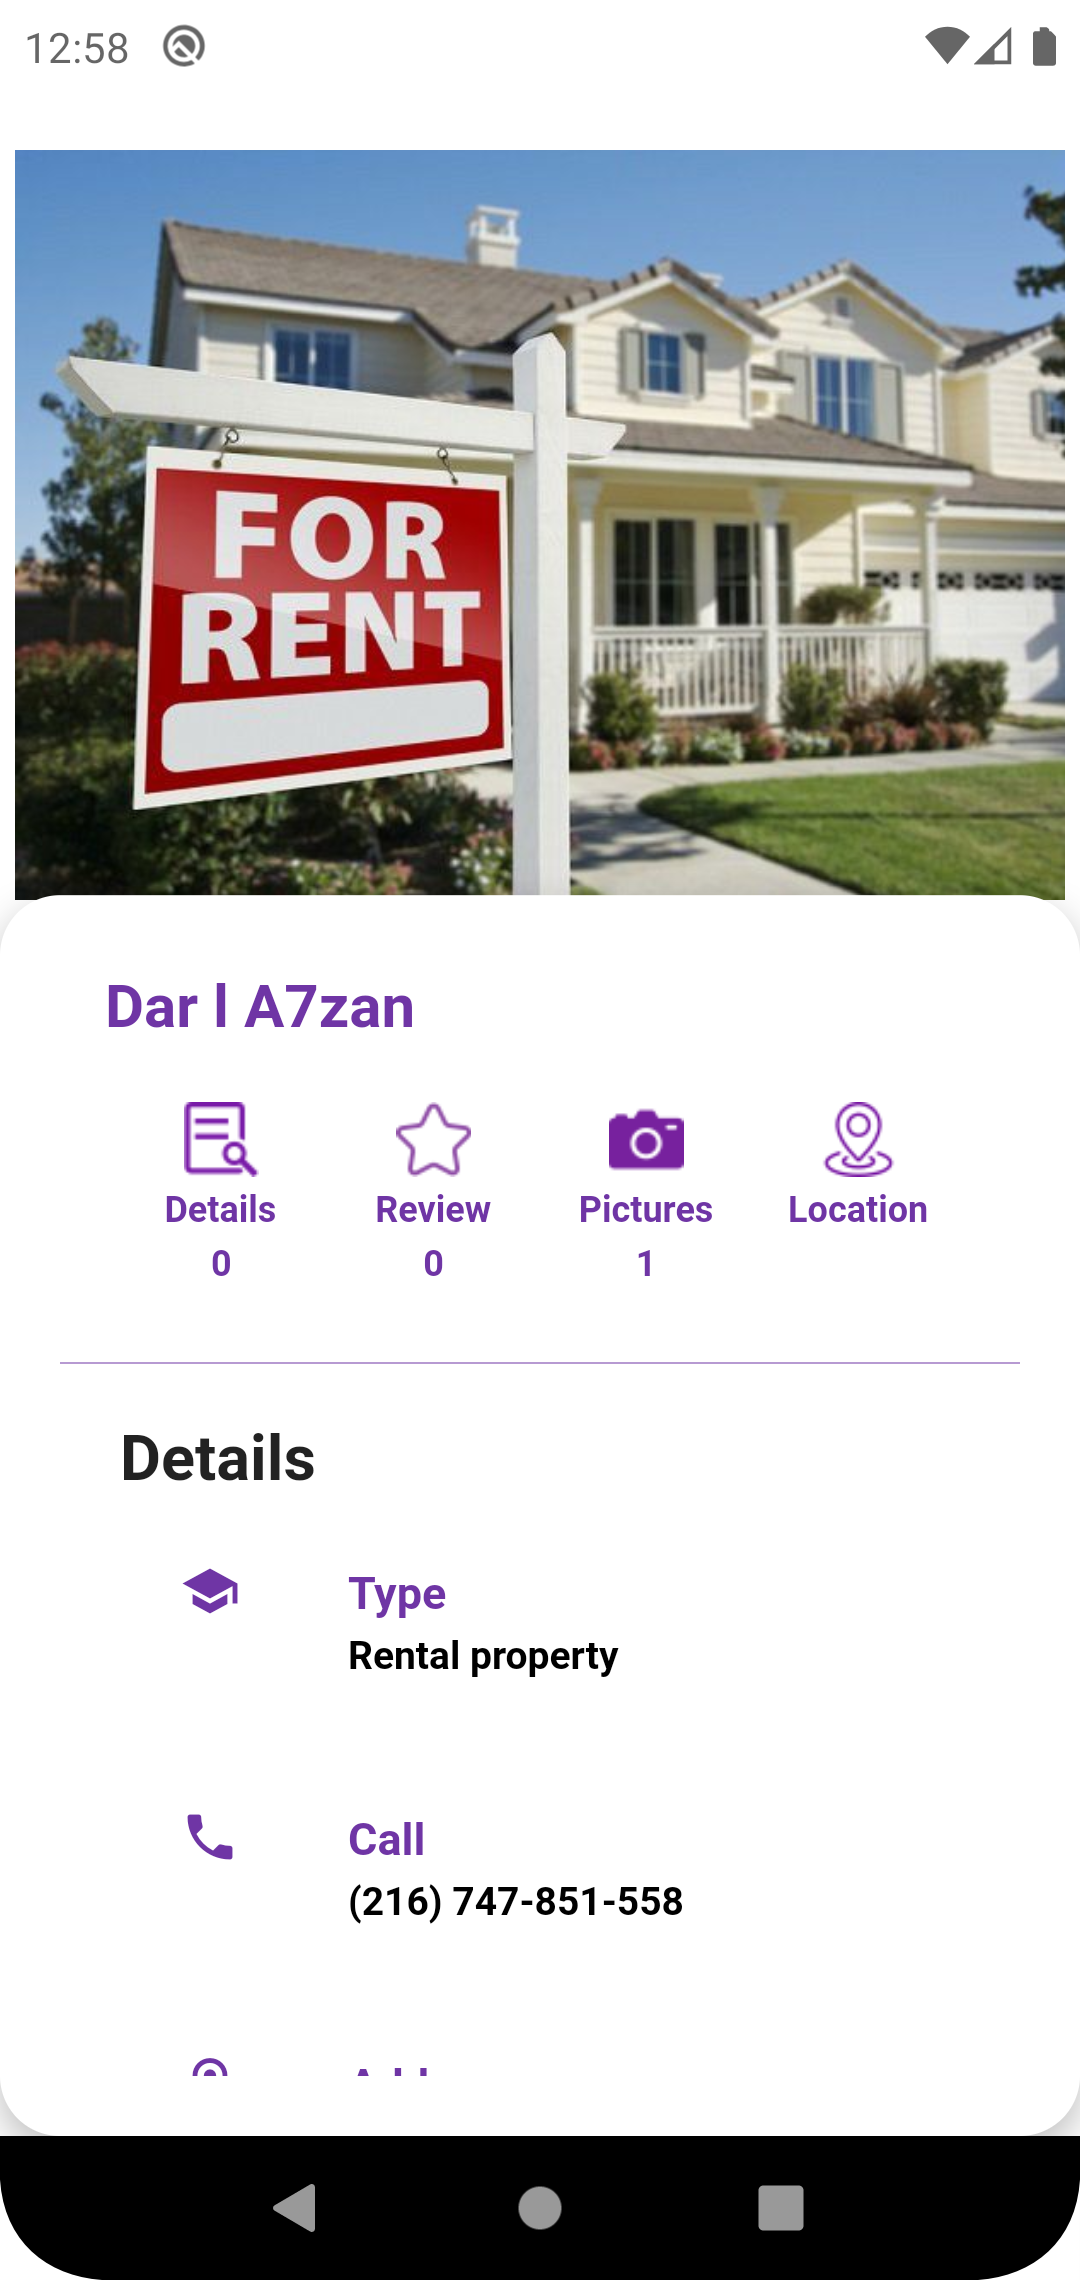
\includegraphics[height=9cm,width=7cm]{images/AAAFacilityDetails.png}
    }
    \caption{l'Interfaces d'endroit }
\end{figure}
\vspace{-1.8cm}
\subsection{Détails Université dans l'application Mobile}
\vspace{-6mm}
L'interface "Détails Université" de l'appli mobile fournit un aperçu complet d'une université.
\vspace{-4mm}
\begin{figure}[H]%
    \center%
    \setlength{\fboxsep}{5pt}%
    \setlength{\fboxrule}{0.5pt}%
    \fbox{
    
\includegraphics[height=9cm,width=7cm]{images/AAAUniversityDetails1.png}
    }
    \caption{l'Interfaces du page profile }
\end{figure}
\vspace{-1.8cm}
\subsection{Partie examen dans l'application mobile}
\vspace{-4mm}
IL'utilisateur de l'application mobile peut consulter les examens, les télécharger et les filtrer.

\begin{figure}[h]
    \centering
    \begin{minipage}[b]{0.45\linewidth}
        \centering
        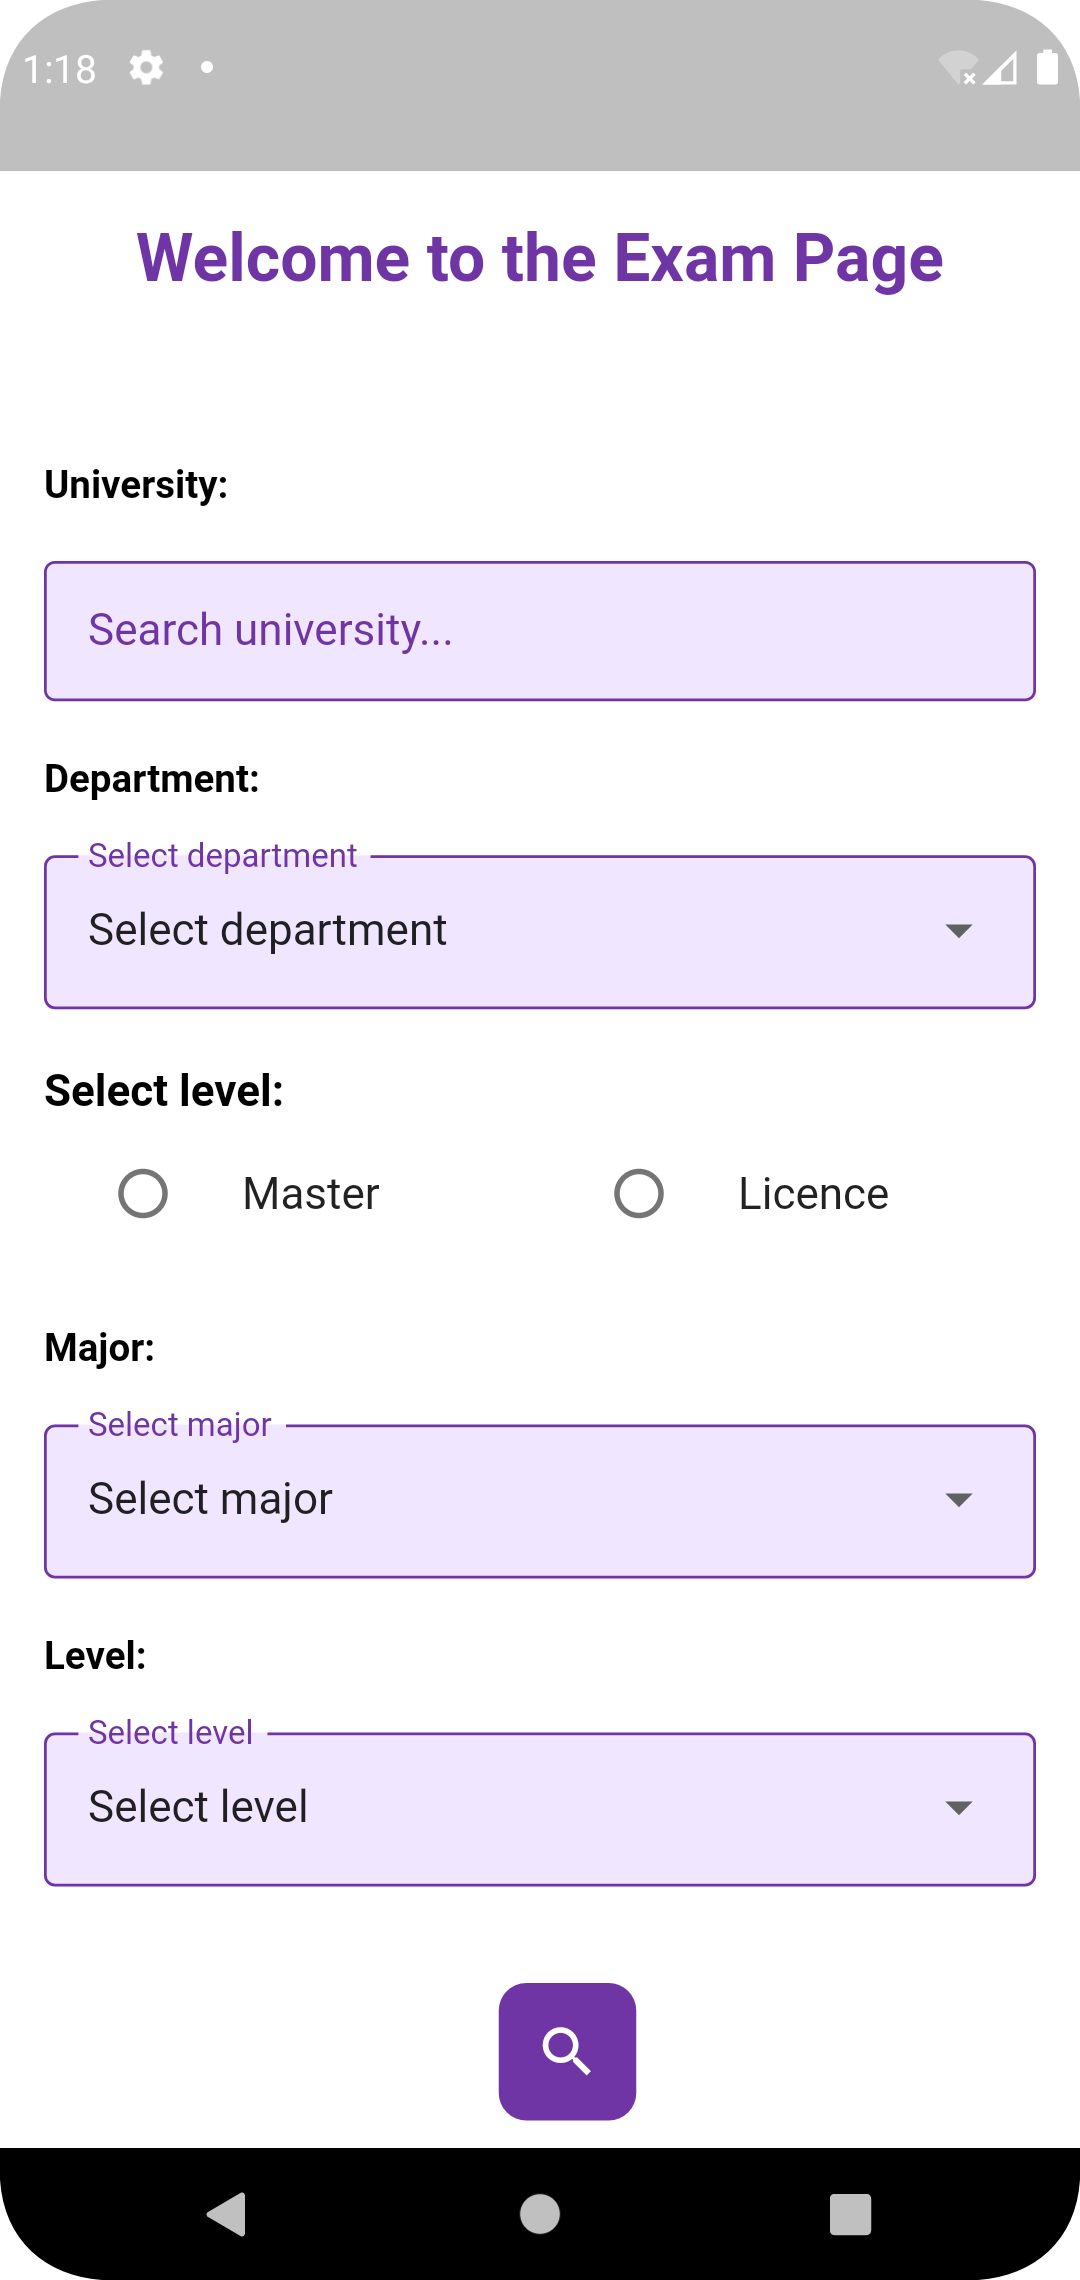
\includegraphics[height=10cm,width=7cm]{images/FilterExamsPage.png}
        \caption{Filtarage des examens}
        \label{fig:image1}
    \end{minipage}
    \hfill
    \begin{minipage}[b]{0.45\linewidth}
        \centering
        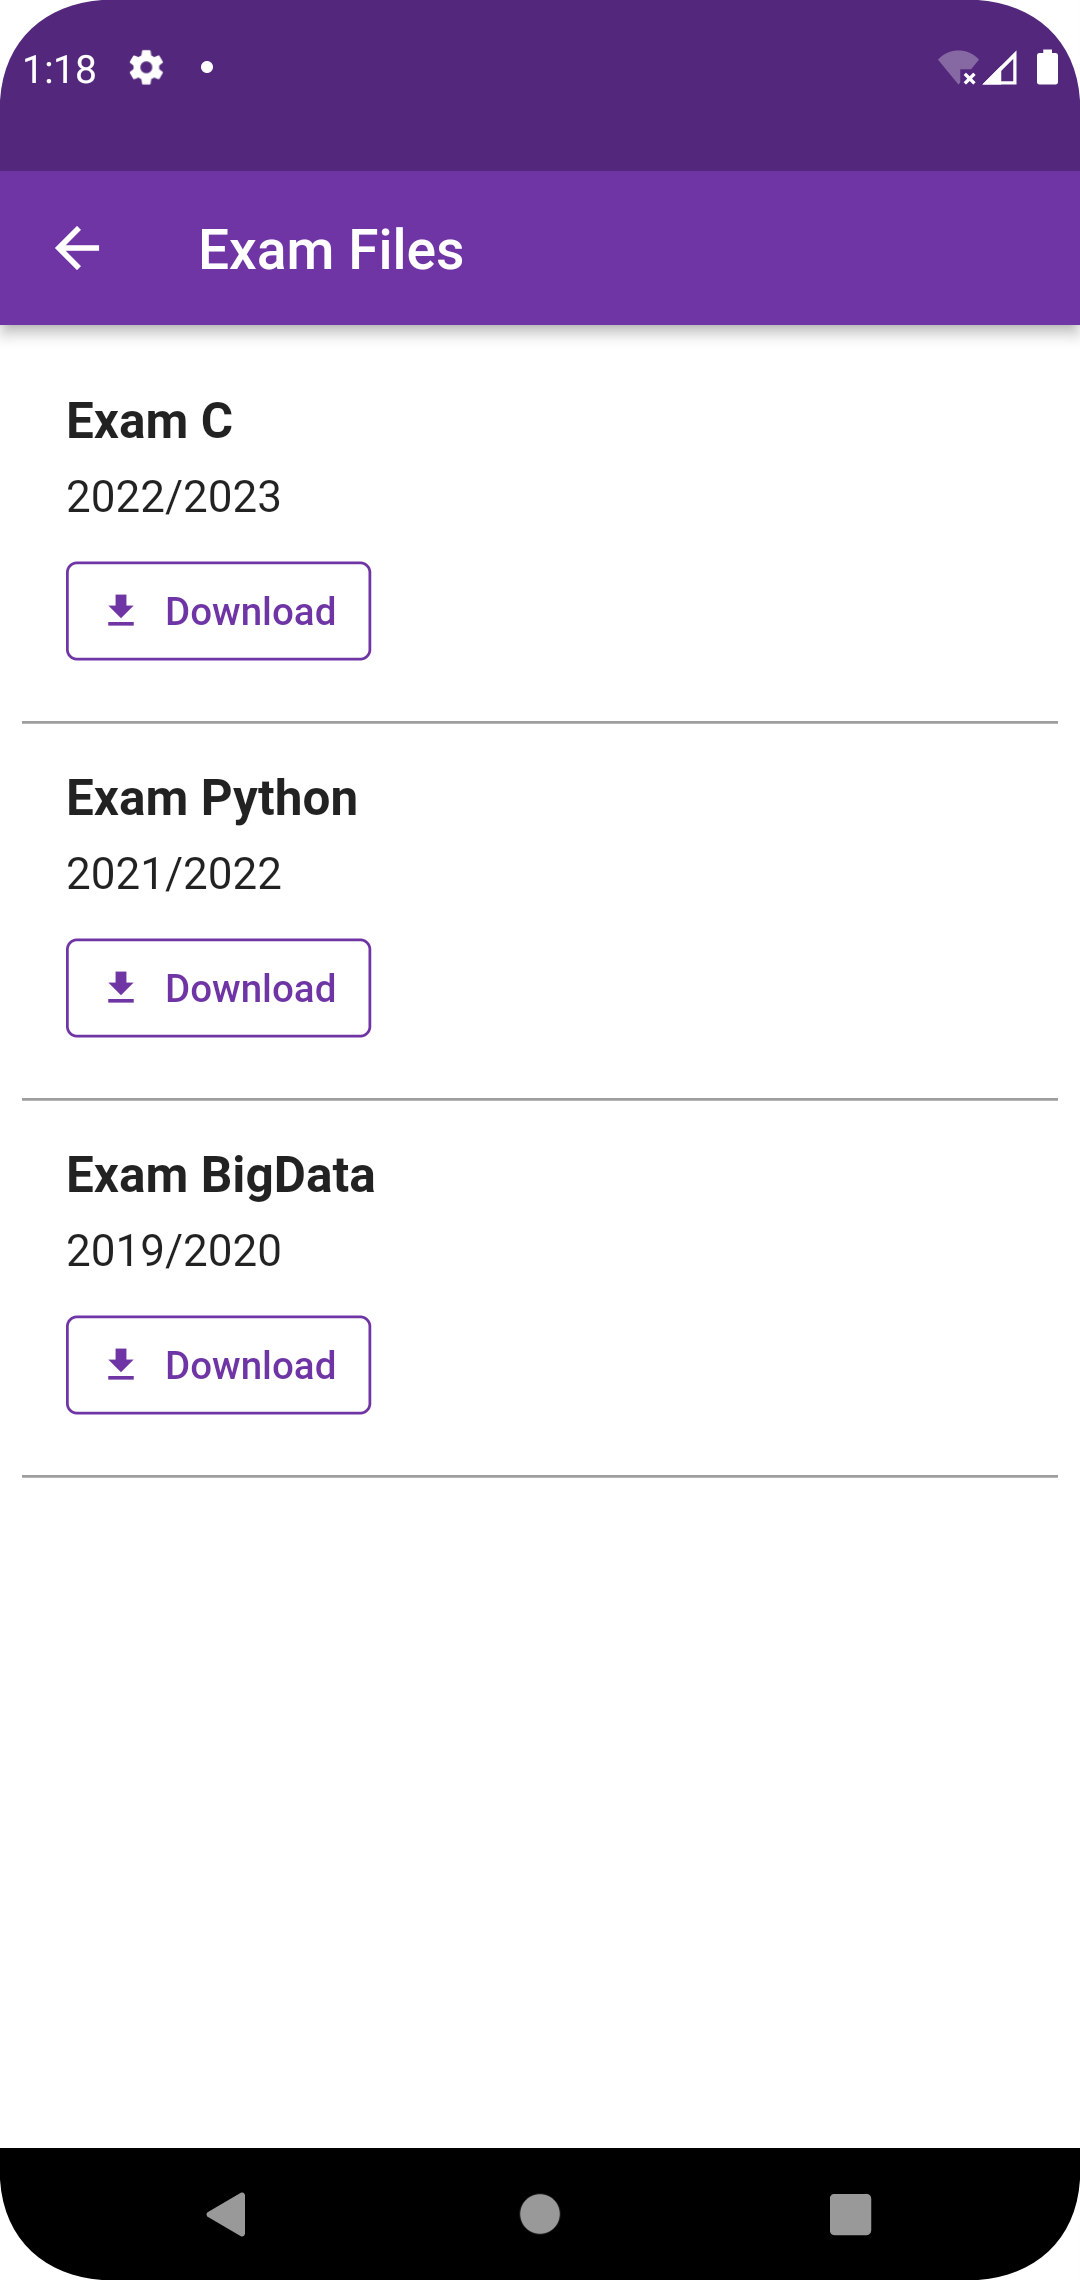
\includegraphics[height=10cm,width=7cm]{images/ExamsPage.png}
        \caption{List des exmanes \\
        }
        \label{fig:image2}
    \end{minipage}
\end{figure}
\vspace{-9mm}
\section{Conclusion }

En conclusion, ce sprint se concentre sur l'amélioration de la gestion des universités, des Endroits et des examens, afin de garantir une expérience utilisateur optimale sur l'application mobile. En dotant les admin d'outils sécurisés, nous visons à simplifier les processus admin, à assurer une gestion fluide des informations critiques et à offrir une visibilité claire et accessible des examens pour tous les utilisateurs. Ce sprint est une étape essentielle pour renforcer l'efficacité et la transparence de notre application.
\end{sloppypar} 

    \chapter{ Chapitre 6 :Sprint 3 " Gestion des  \centering Transports ,Evénement et des Stages"}
\begin{spacing}{1.2}
\minitoc
\thispagestyle{MyStyle}
\end{spacing}
\newpage
\begin{sloppypar} 

\section{Introduction }
\vspace{-4mm}
Le prochain sprint sera axé sur la gestion du transport, des événements et des stages au sein de notre application. L'objectif est de fournir aux admins les outils nécessaires pour organiser et superviser efficacement ces aspects. Ce sprint vise à améliorer l'efficacité administrative et à offrir une meilleure expérience utilisateur.

\vspace{-9mm}
\section{Backlog du sprint}
\vspace{-4mm}
Le backlog de gestion des transports, des événements et des stages propose une série de tâches visant à faciliter la gestion de ces éléments au sein de notre application. Cela comprend l'ajout, la modification et la suppression de transports, d'événements et de stages, ainsi que la consultation de ces informations par les utilisateurs.
\vspace{-3mm}
\begin{table}[h]
\centering
\begin{tabular}{|p{10cm}|p{2cm}|p{2.5cm}|}
\hline
\textbf{ Tâches } & \textbf{ Priorité }& \textbf{Période/jour}  \\
\hline
En tant qu’un admin je peux gérer les offres du stages dans l’application web. & Élevée  & 4 jours  \\
\hline
En tant qu’un admin je peux gérer les stations de transports dans l’application web. & Moyenne  & 3 jours  \\
\hline
En tant qu’un admin je peux gérer les événements dans l’application web. & Élevée & 4 jours \\
\hline
En tant qu’un utilisateur je peux consulter  les offres du stages dans l’application mobile. & Élevée  & 3 jours \\
\hline
En tant qu’un utilisateur je peux consulter  les stations de transports dans l’application mobile. & Moyenne & 1 jour\\
\hline
En tant qu’un utilisateur je peux consulter  les événements dans l’application mobile. & Moyenne & 1 jour\\
\hline
\end{tabular}
\caption{Tableau de Backlog de produit Sprint 3}
\end{table}
\vspace{-1.2cm}
\section {Analyse et spécification des besoins}
\vspace{-4mm}
Afin de mieux comprendre la structure de notre système, nous avons utilisé un diagramme de cas d'utilisations qui est présenté ci-dessous.
\vspace{-4mm}

\subsection{Diagramme de classes }
\vspace{-4mm}

Le diagramme de cas d'utilisation illustre les différentes actions qu'un admin peut effectuer sur la gestion des transports, des événements et des stages via l'interface web de l'application.
\vspace{-4mm}
\begin{figure}[H]%
    \center%
    \setlength{\fboxsep}{5pt}%
    \setlength{\fboxrule}{0.5pt}%
    \fbox{
    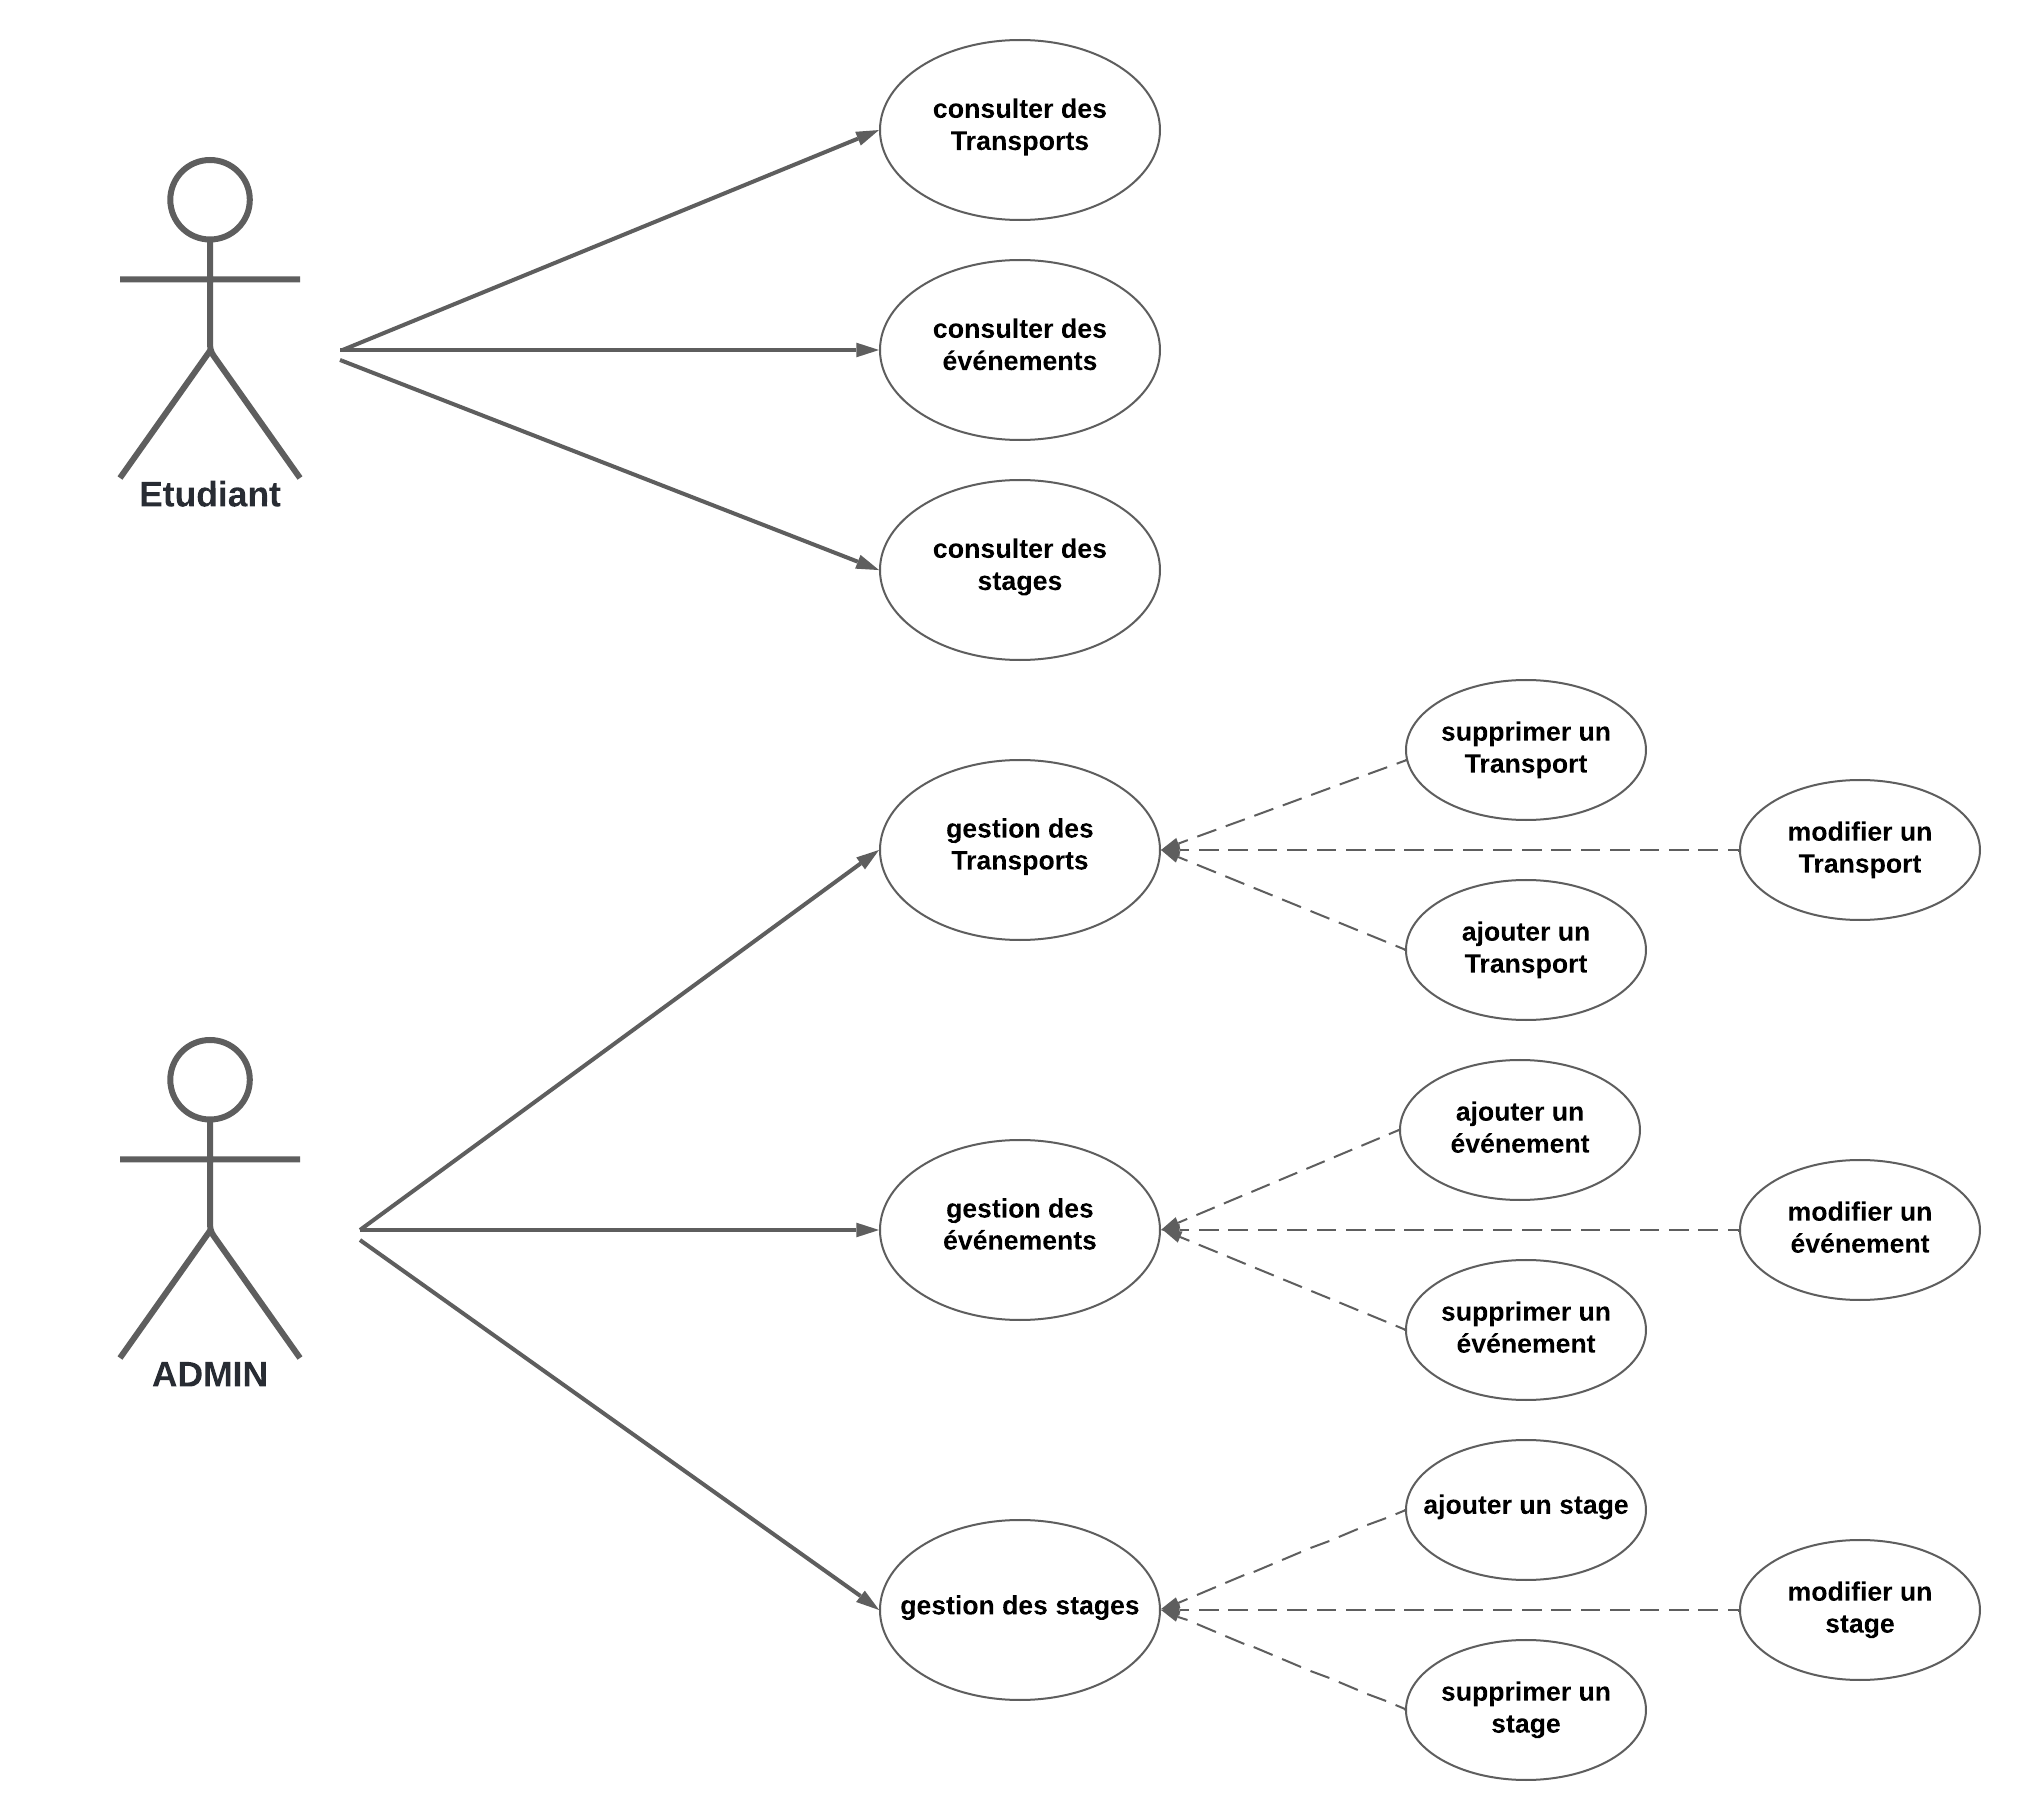
\includegraphics[height=23cm,width=15cm]{images/gestion des transport, evenements et stages.png}%
    }
    \caption{Figure du Diagramme de cas d'utilisation Sprint 3 }
\end{figure}

\subsection{Description textuelle du cas d’utilisation «Ajouter un stage»}
\vspace{-4mm}

l'admin peut saisir les détails d'un nouveau stage, vérifier les informations et les enregistrer dans le système.

\begin{table}[h]
\centering
\begin{tabular}{|p{3cm}|p{12cm}|}
\hline
\textbf{Cas d'utilisation } & Ajouter un stage \\
\hline
\textbf{Acteurs} & Admin \\
\hline
\textbf{Précondition} & Admin authentifié \\
\hline
\textbf{Postcondition} & Stage ajouté \\
\hline
\textbf{Scénario nominal} &
\begin{enumerate}
    \item L'admin est sur la page d'accueil.
    \item L'admin choisit "Stages" dans la barre latérale.
    \item L'admin clique sur le bouton "Ajouter un stage".
    \item Le système affiche le formulaire d'ajout de stage.
    \item L'admin remplit le formulaire avec les détails du stage.
    \item L'admin soumet le formulaire.
    \item Le système enregistre les informations du stage et le stage est ajouté à la liste des stages disponibles.
\end{enumerate} \\
\hline
\textbf{Exception} & Le système affiche un message d'erreur si un champ obligatoire n'est pas rempli dans le formulaire d'ajout de stage. \\
\hline 
\end{tabular}
\caption{Description du cas d’utilisation « Ajouter un stage »}
\end{table}

\vspace{-1.3cm}

\subsection{Description textuelle du cas d’utilisation «Modifier un stage»}
\vspace{-4mm}
l'admin peut saisir les détails d'un nouveau stage, vérifier les informations et les enregistrer dans le système.

\begin{table}[h]
\centering
\begin{tabular}{|p{3cm}|p{12cm}|}
\hline
\textbf{Cas d'utilisation } & Modifier un stage \\
\hline
\textbf{Acteurs} & Admin \\
\hline
\textbf{Précondition} & Admin authentifié \\
\hline
\textbf{Postcondition} & Stage modifié \\
\hline
\textbf{Scénario nominal} &
\begin{enumerate}
    \item L'admin est sur la page d'accueil.
    \item L'admin choisit "Stages" dans la barre latérale.
    \item L'admin consulte la liste des stages.
    \item L'admin sélectionne le stage à modifier.
    \item Le système affiche le formulaire de modification de stage.
    \item L'admin modifie les détails du stage.
    \item L'admin soumet le formulaire de modification.
    \item Le système enregistre les modifications et le stage est mis à jour dans la liste des stages disponibles.
\end{enumerate} \\
\hline
\textbf{Exception}& Un champ obligatoire n'est pas rempli. Le système affiche un message d'erreur si un champ obligatoire n'est pas rempli dans le formulaire de modification de stage. \\
\hline 
\end{tabular}
\caption{Description du cas d’utilisation « Modifier un stage »}
\end{table}

\newpage

\subsection{Description textuelle du cas d’utilisation «Supprimer un stage»}
\vspace{-6mm}
l'admin peut retirer un stage existant de la base de données.
\begin{table}[h]
\centering
\begin{tabular}{|p{3cm}|p{12cm}|}
\hline
\textbf{Cas d'utilisation } & Supprimer un stage \\
\hline
\textbf{Acteurs} & Admin \\
\hline
\textbf{Précondition} & Admin authentifié \\
\hline
\textbf{Postcondition} & Stage supprimé \\
\hline
\textbf{Scénario nominal} &
\begin{enumerate}
    \item L'admin est sur la page d'accueil.
    \item L'admin choisit "Stages" dans la barre latérale.
    \item L'admin consulte la liste des stages.
    \item L'admin sélectionne le stage à supprimer.
    \item Le système affiche une confirmation de suppression.
    \item L'admin confirme la suppression.
    \item Le système supprime le stage de la liste des stages disponibles.
\end{enumerate} \\
\hline
\end{tabular}
\caption{Description du cas d’utilisation « Supprimer un stage »}
\end{table}
\vspace{-1.7cm}
\section{Diagramme de séquence }
\vspace{-6mm}
Les diagrammes de séquence illustrent les interactions lors de la gestion des stages, offrant une vue claire des processus impliqués.
\vspace{-1cm}
\subsection{Diagramme de séquence «Ajouter un Stage»}
\vspace{-6mm}
Le diagramme présente le processus d'ajout d'un nouveau stage par l'admin sur la partie web de notre application.
\vspace{-4mm}
\begin{figure}[H]%
    \center%
    \setlength{\fboxsep}{5pt}%
    \setlength{\fboxrule}{0.5pt}%
    \fbox{
    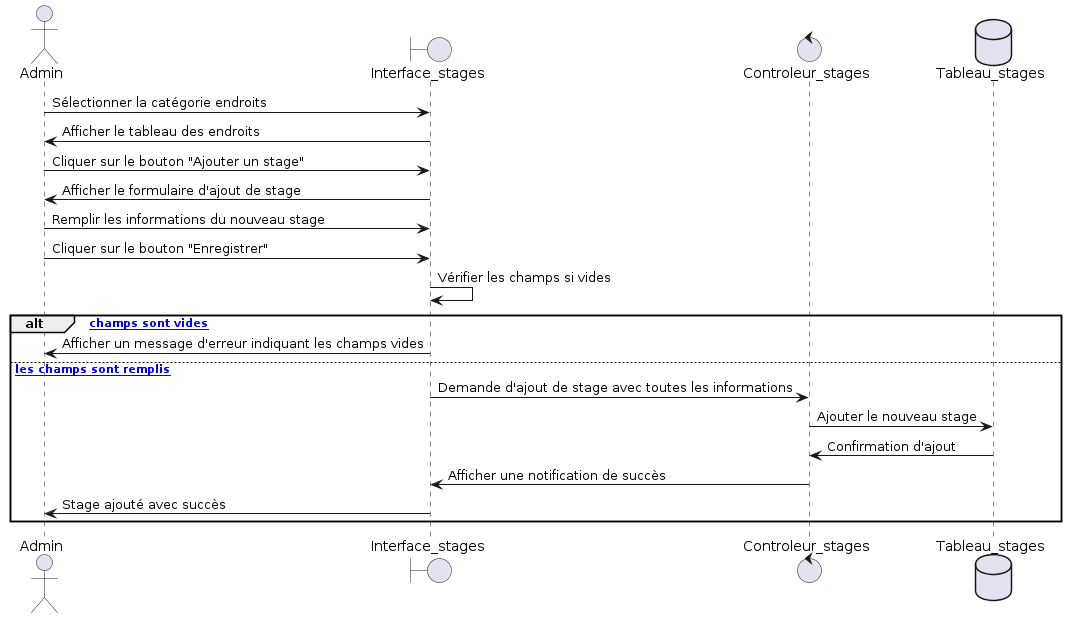
\includegraphics[height=9cm,width=15cm]{images/ffffajoutstages.png}%
    }
    \caption{Figure du Diagramme de séquence «Ajouter un stage» }
\end{figure}

\subsection{Diagramme de séquence «Modifier un Stage»}
\vspace{-6mm}
Le diagramme illustre le processus de modification d'un stage par l'admin sur la partie web de notre application.
\vspace{-4mm}
\begin{figure}[H]%
    \center%
    \setlength{\fboxsep}{5pt}%
    \setlength{\fboxrule}{0.5pt}%
    \fbox{
    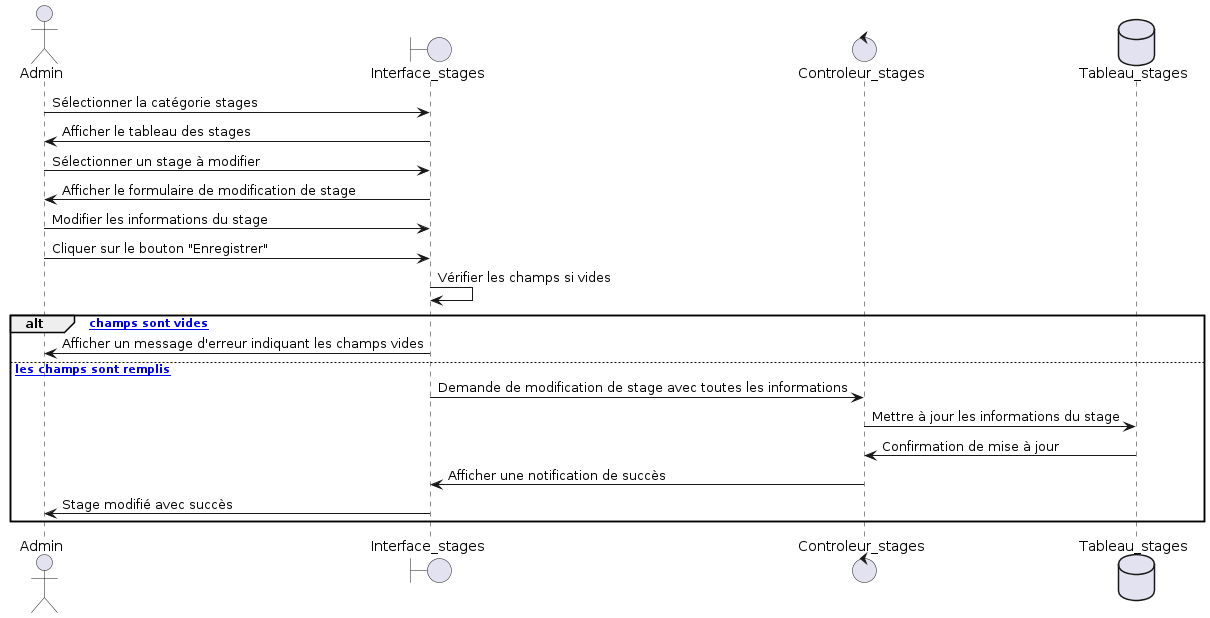
\includegraphics[height=8.5cm,width=15cm]{images/ffffeditstage.png}%
    }
    \caption{Diagramme de séquence «modifier un stage» }
\end{figure}
\vspace{-1.7cm}
\subsection{Diagramme de séquence «Supprimer un Stage»}
\vspace{-6mm}
Le diagramme décrit le processus de suppression d'un stage par l'admin sur la partie web de notre application.
\vspace{-2mm}
\begin{figure}[H]%
    \center%
    \setlength{\fboxsep}{5pt}%
    \setlength{\fboxrule}{0.5pt}%
    \fbox{
    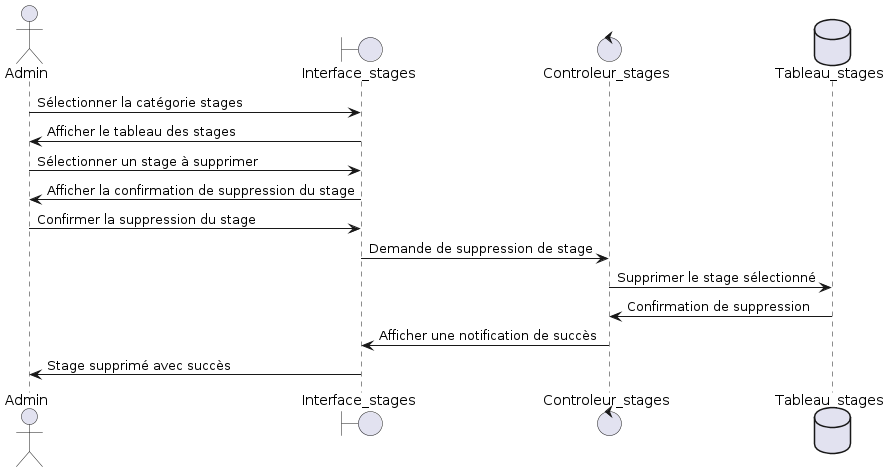
\includegraphics[height=8.5cm,width=15cm]{images/fffffsuppstage.png}%
    }
    \caption{Diagramme de séquence supprimer un stage }
\end{figure}
\vspace{-7mm}
\section{Diagramme de classes }
\vspace{-4mm}
Le diagramme de classes présenté ci-dessus illustre la structure des entités clés de notre système de gestion, à savoir les stages, les événements et les transports. Chaque entité est représentée par une classe correspondante, comprenant des attributs décrivant ses caractéristiques principales ainsi que des méthodes pour accéder et manipuler ces données. Cette conception permet une modélisation claire et cohérente des différentes fonctionnalités de notre application.

\begin{figure}[H]%
    \center%
    \setlength{\fboxsep}{5pt}%
    \setlength{\fboxrule}{0.5pt}%
    \fbox{
    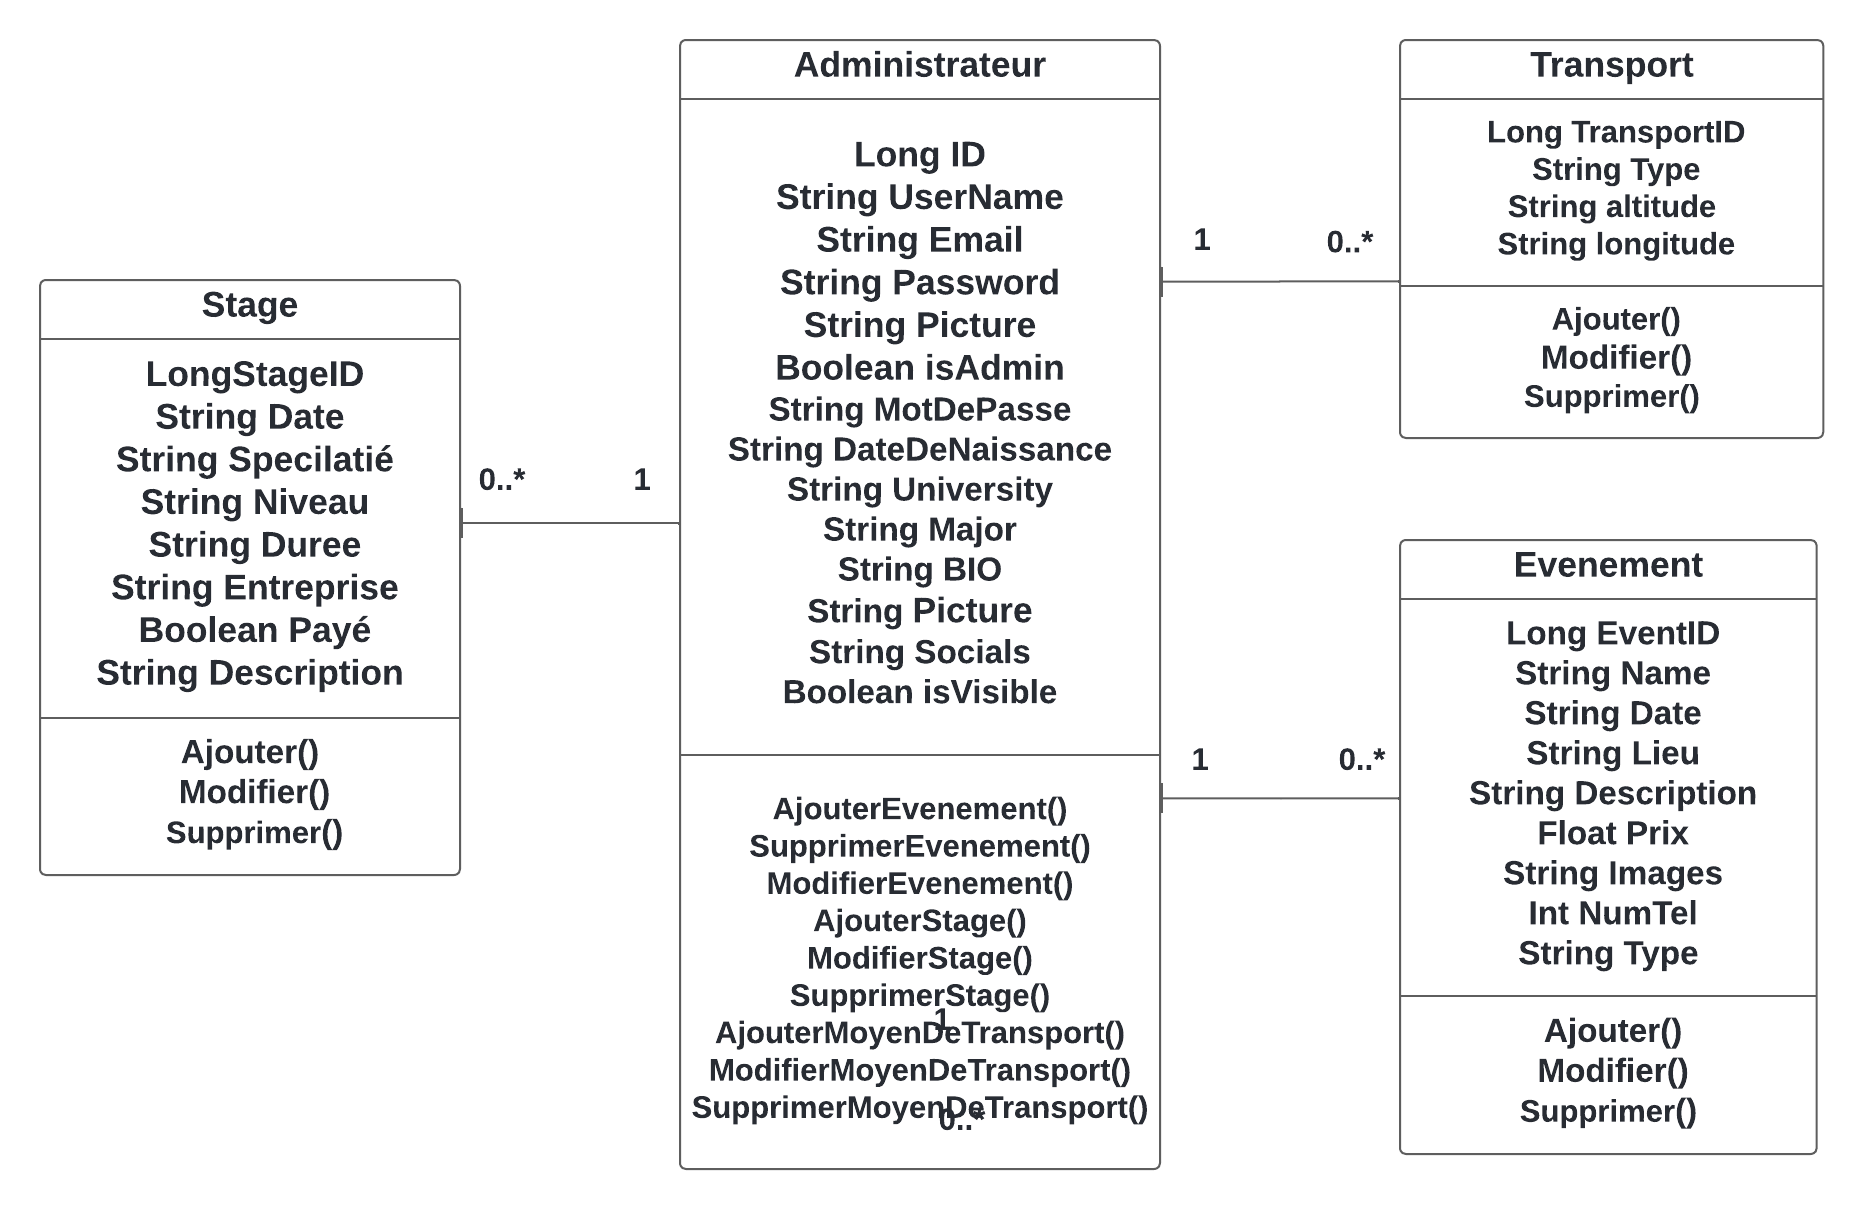
\includegraphics[height=16.5cm,width=15cm]{images/AAATransportations.png}%
    }
    \caption{Diagramme de classes Sprint 3}
\end{figure}
\vspace{-4mm}
\section{Réalisation }
\vspace{-4mm}
La partie de réalisation représente la dernière phase du cycle de développement d’un sprint. Elle permet de présenter les résultats obtenus lors de l’étape de développement afin d’assurer et de garantir une version de qualité. Nous allons montrer cela par des captures d’écrans des fonctionnalités ayant été développées.

\vspace{-9mm}
\subsection{Ajout d'un évenement}
\vspace{-4mm}
L'interface web pour l'admin permet d'ajouter des événements. Via le menu de navigation, l'admin accède à un formulaire pour entrer le titre, la description, la date, l'heure et le lieu de l'événement. Une fois soumis, l'événement est visible pour les utilisateurs de l'application mobile.

\begin{figure}[h]
    \centering
    \begin{minipage}[b]{0.45\linewidth}
        \centering
        \setlength{\fboxsep}{5pt}%
        \setlength{\fboxrule}{0.5pt}%
        \fbox{
        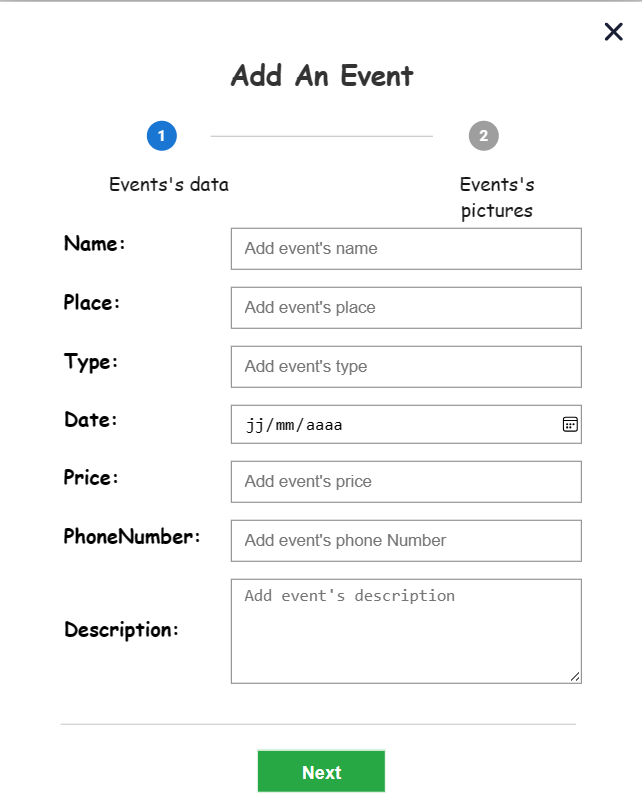
\includegraphics[height=12cm,width=8cm]{images/XAddEvent1.png}
        }
        \caption{Interface d'ajout d'un évenement}
        \label{fig:image1}
    \end{minipage}
    \hfill
    \begin{minipage}[b]{0.45\linewidth}
        \centering
        \setlength{\fboxsep}{5pt}%
        \setlength{\fboxrule}{0.5pt}%
        \fbox{
        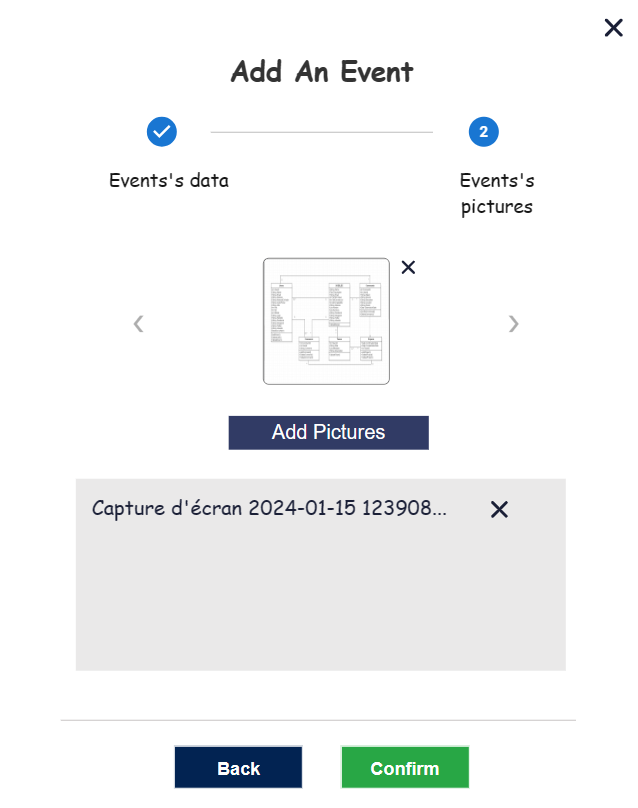
\includegraphics[height=12cm,width=8cm]{images/XAddEvent2.png}
        }
        \caption{Diagramme de classes publication et notification}
        \label{fig:image2}
    \end{minipage}
\end{figure}


\subsection{Modification d'un stage}
\vspace{-6mm}
L'admin peut modifier les détails des stages via l'interface web, incluant titre, description, durée, exigences et lieu, visibles immédiatement sur l'application mobile.
\vspace{-4mm}
\begin{figure}[H]%
    \center%
    \setlength{\fboxsep}{5pt}%
    \setlength{\fboxrule}{0.5pt}%
    \fbox{
    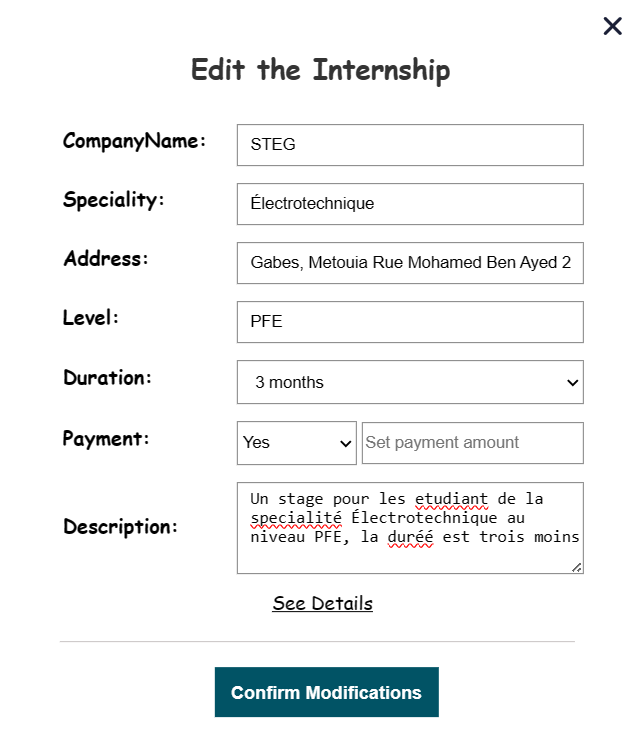
\includegraphics[height=10cm,width=10cm]{images/XEditInternship.png}%
    }
    \caption{Interface de modification d'un stage}
\end{figure}
\vspace{-1.9Cm}
\section{Effacer un moyen du transport }
\vspace{-6mm}
L'interface web admin permet de supprimer des transports en sélectionnant et confirmant leur suppression de l'application mobile.
\vspace{-4mm}
\begin{figure}[H]%
    \center%
    \setlength{\fboxsep}{5pt}%
    \setlength{\fboxrule}{0.5pt}%
    \fbox{
    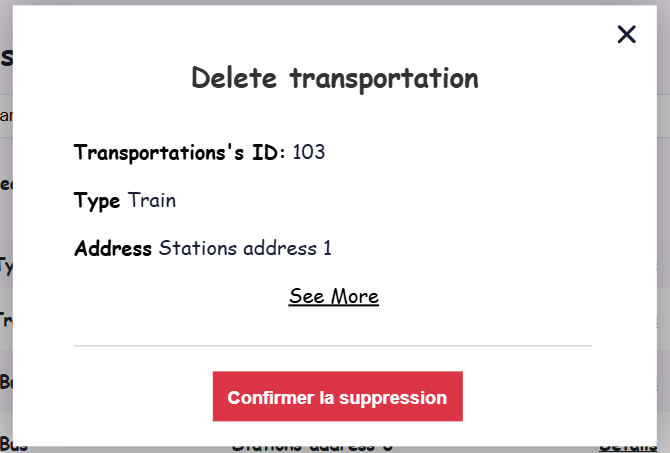
\includegraphics[height=7cm,width=13cm]{images/AAADeleteTrasportation.png}%
    }
    \caption{Interface de supression d'un stage}
\end{figure}
\vspace{-1.3cm}
\subsection{Evenement partie Mobile }
\vspace{-6mm}
Sur l'application mobile, les utilisateurs peuvent consulter les  événements, incluant le titre, la description, la date, l'heure, le lieu, ainsi que les images associées à chaque événement.
\vspace{-2mm}
\begin{figure}[H]%
    \center%
    \setlength{\fboxsep}{5pt}%
    \setlength{\fboxrule}{0.5pt}%
    \fbox{
    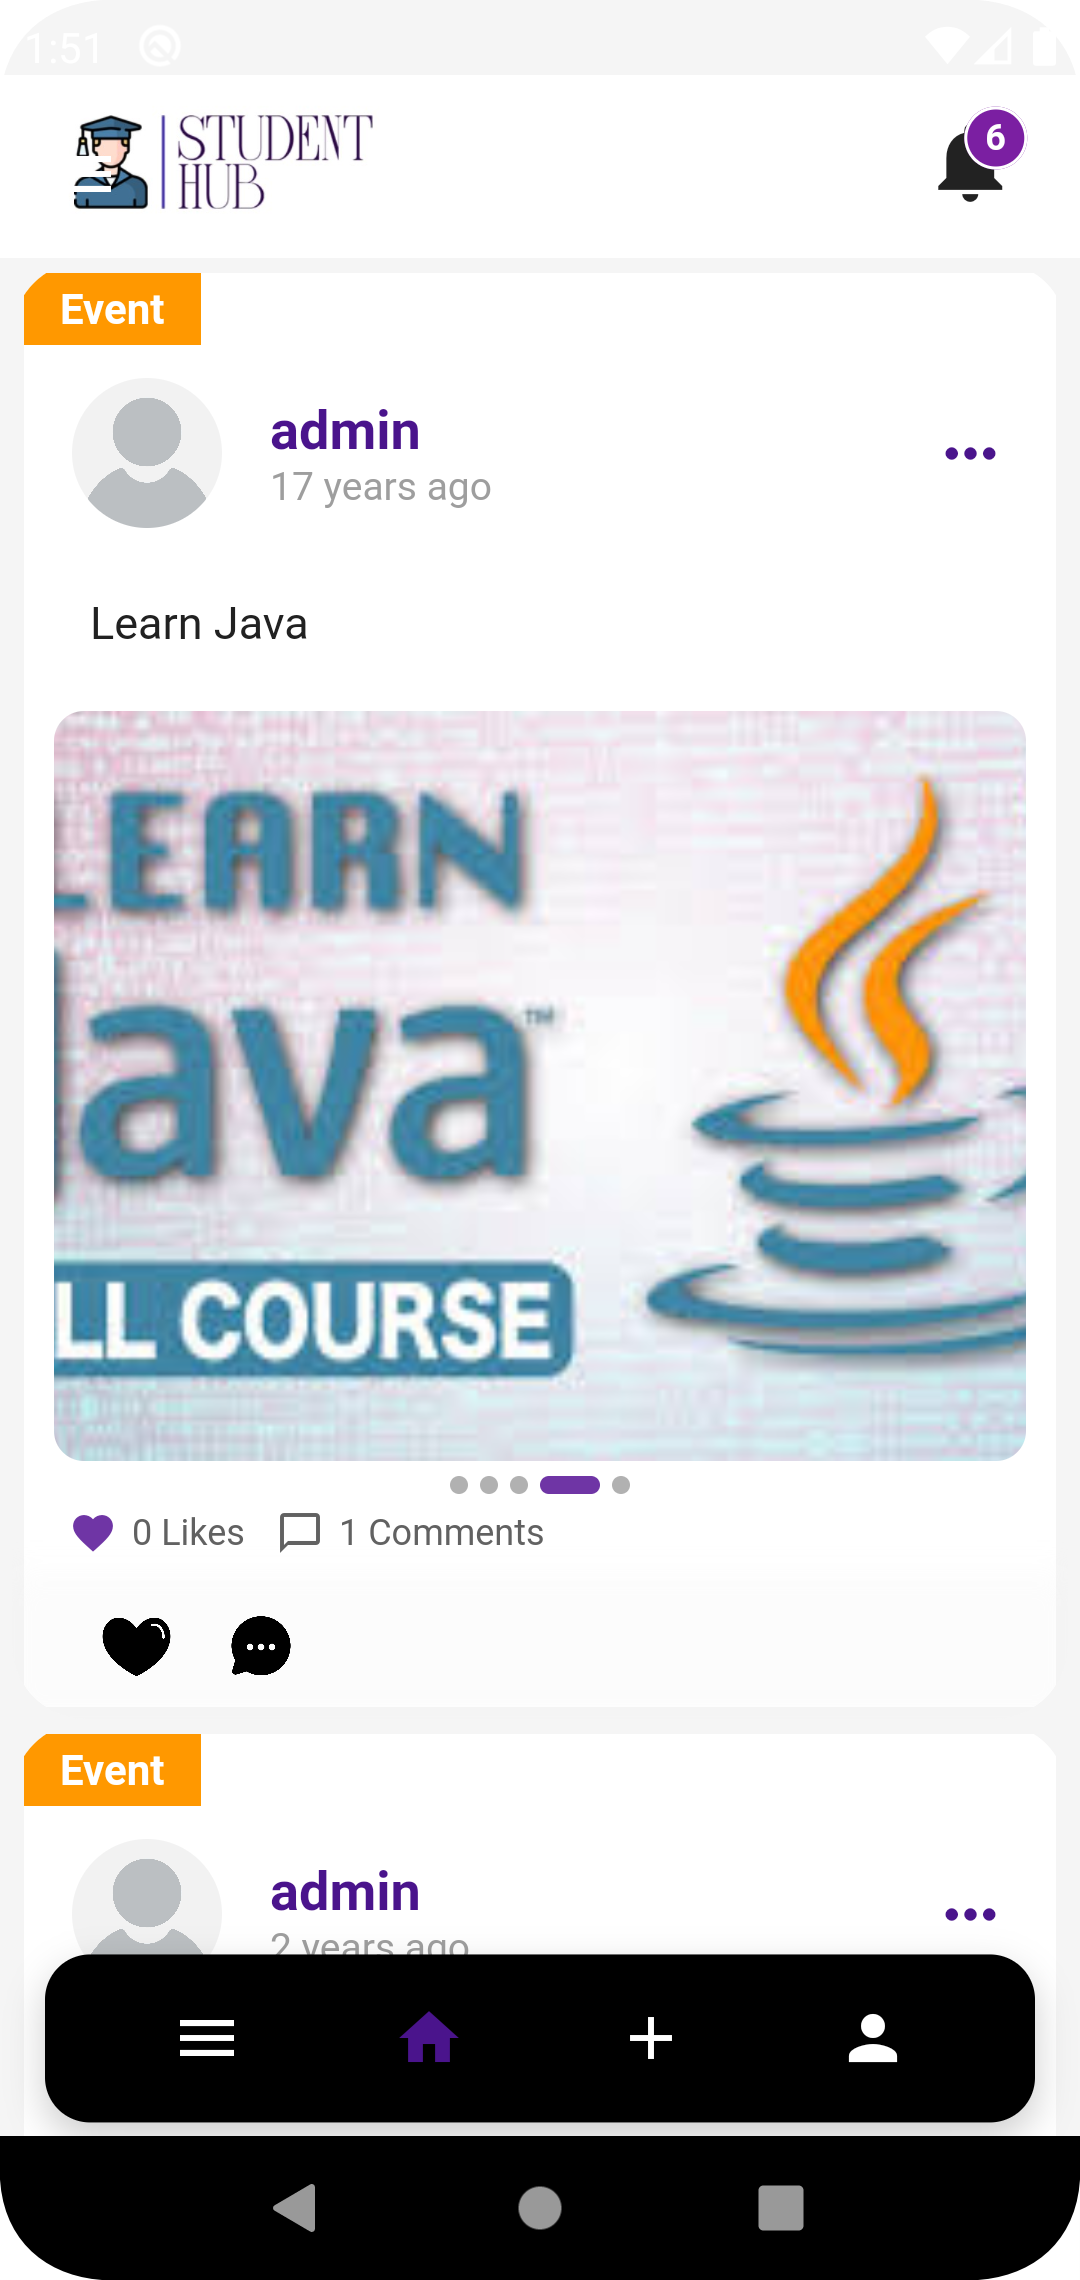
\includegraphics[height=8.7cm,width=7cm]{images/AAAEventPublication.png}%
    }
    \caption{Interface d'un évenement dans la partie mobile}
\end{figure}
\vspace{-1.8Cm}
\subsection{Stage partie mobile }
\vspace{-6mm}
Les utilisateurs peuvent voir les détails des offres de stages, y compris le titre, la description, les qualifications requises, les dates et le lieu.
\vspace{-2mm}
\begin{figure}[H]%
    \center%
    \setlength{\fboxsep}{5pt}%
    \setlength{\fboxrule}{0.5pt}%
    \fbox{
    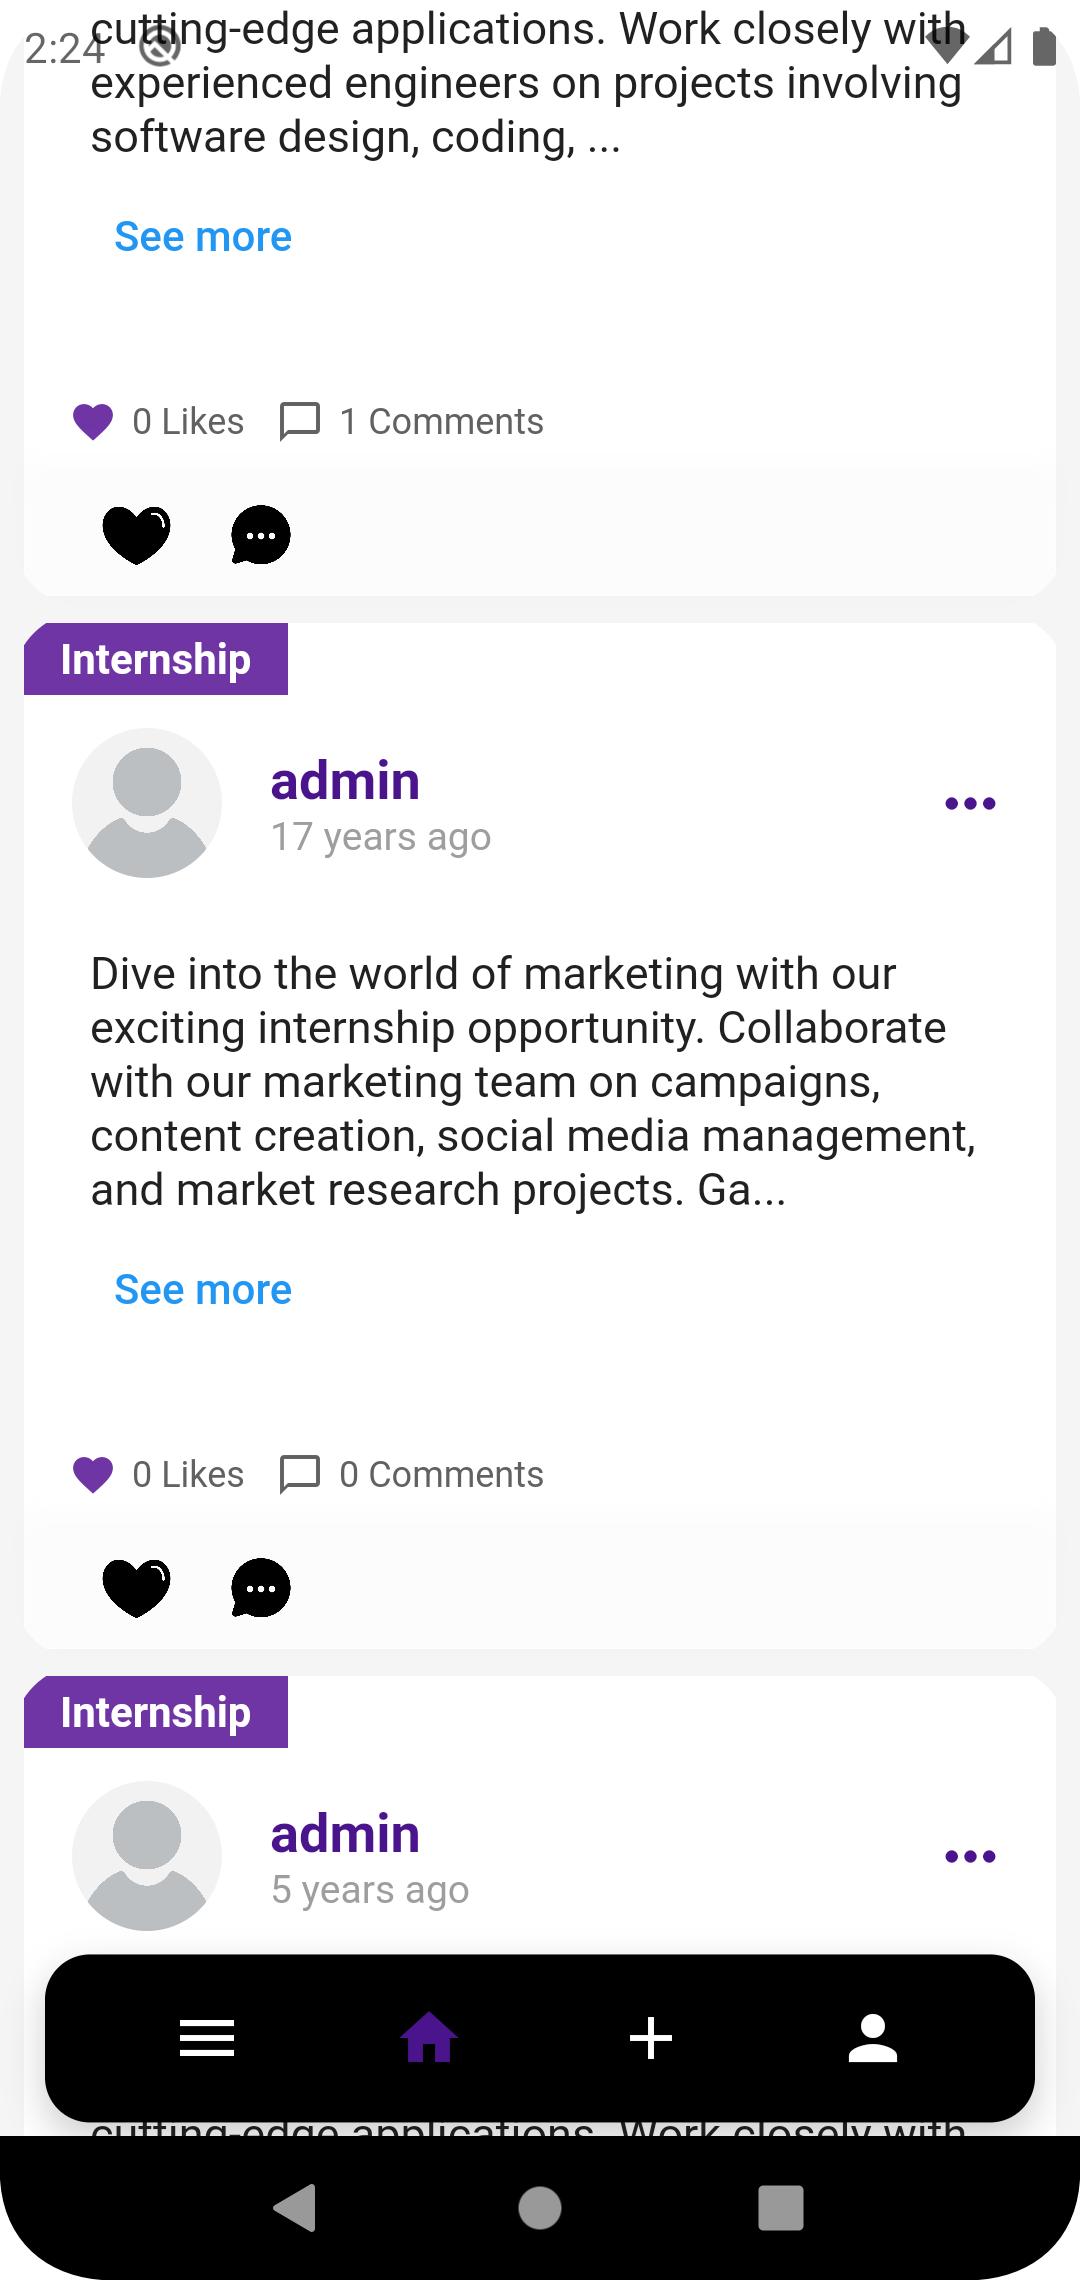
\includegraphics[height=8.7cm,width=7cm]{images/AAAInternshipPublications.png}%
    }
    \caption{Interface d'un stage dans la partie mobile}
\end{figure}
\vspace{-1cm}
\subsection{Les moyens des transports partie mobile }
\vspace{-4mm}
Sur l'application mobile, les utilisateurs peuvent consulter les informations sur les transports. Chaque entrée affiche les détails tels que le type de transport, les horaires et les itinéraires. Les utilisateurs peuvent également voir les mises à jour en temps réel sur les retards ou les changements de service.
\begin{figure}[H]%
    \center%
    \setlength{\fboxsep}{5pt}%
    \setlength{\fboxrule}{0.5pt}%
    \fbox{
    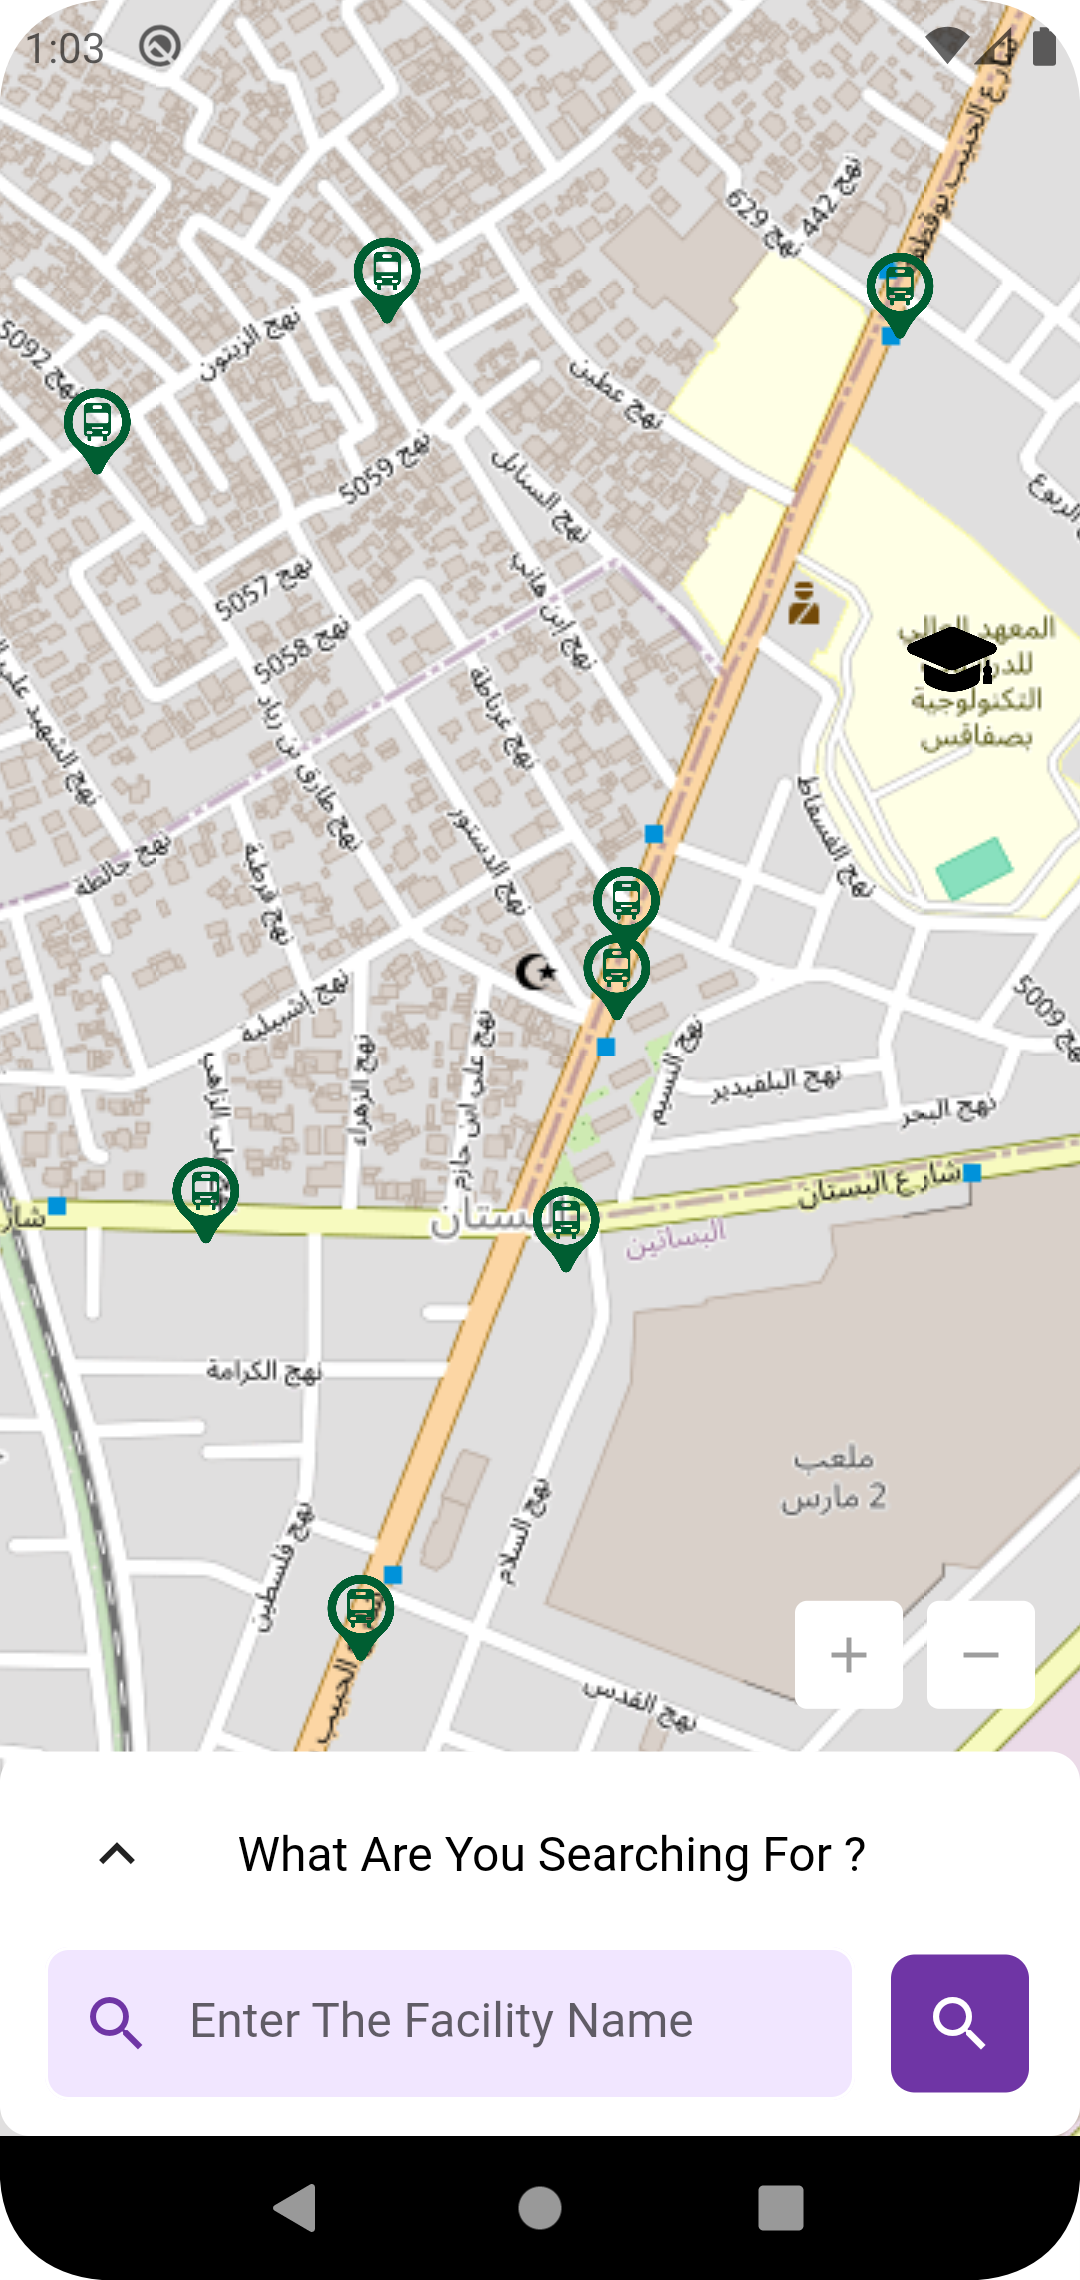
\includegraphics[height=10cm,width=7cm]{images/AAATransportStations.png}%
    }
    \caption{Interface du moyen de transport dans la partie mobile}
\end{figure}

\vspace{-1cm}

\section{Conclusion }
\vspace{-4mm}
En conclusion, ce sprint se focalise sur l'optimisation de la gestion du transport, des événements et des stages au sein de notre application. En dotant les admins d'outils performants et intuitifs, nous visons à améliorer l'affichage des moyens transports disponibles, à faciliter l'organisation et la communication autour des événements, et à simplifier l'accès aux opportunités de stage pour les utilisateurs. Ce sprint représente une étape clé pour renforcer l'efficacité administrative et offrir une expérience utilisateur enrichie et fluide.

\end{sloppypar} 

    \chapter{ Chapitre 7 : Sprint 4 "Gestion \centering des Publications   et des Notifications"}
\begin{spacing}{1.2}
\minitoc
\thispagestyle{MyStyle}
\end{spacing}
\newpage
\begin{sloppypar} 

\section{Introduction }
\vspace{-4mm}
Dans ce sprint, nous nous concentrons sur l'amélioration de nos publications et notifications pour une expérience utilisateur plus engageante. Nous travaillerons sur l'optimisation de l'interface de publication, l'ajout de fonctionnalités de réaction, ainsi que sur l'amélioration de la gestion des notifications pour une distribution plus ciblée. 

\vspace{-1cm}
\section{Backlog du sprint}
\vspace{-4mm}
Le backlog de gestion des publications et des notifications comprend des tâches telles que la création, la modification et la suppression de publications, ainsi que la gestion des notifications automatiques et personnalisées. Cela permettra de garantir une diffusion efficace de l'information et une interaction fluide entre les utilisateurs et l'application.
\vspace{-1mm}
\begin{table}[h]
\centering
\begin{tabular}{|p{8cm}|p{3cm}|p{3cm}|}
\hline
\textbf{ Tâches } & \textbf{ Priorité }& \textbf{Période/jour}  \\
\hline En tant qu’un étudiant ,je peux consulter les publications de ma page d’accueil dans l’application mobile.& Élevée  & 5 jours \\
\hline En tant qu’un étudiant ,je peux consulter mes publications de ma page profile dans l’application mobile.  & Élevée  & 4 jours  \\
\hline En tant qu’un étudiant ,je peux commenter et réagir aux publications dans l’application mobile.  & Élevée  & 7 jours  \\
\hline En tant qu’un étudiant ,je peux supprimer mes publications dans l’application mobile.  & Élevée  & 7 jours  \\
\hline En tant qu'un utilisateur, je peux créer  des notifications personnalisés  sur la partie web  & Élevée  & 7 jours  \\
\hline En tant qu’un étudiant ,je peux commenter et réagir aux publications dans l’application mobile.  & Élevée  & 7 jours  \\
\hline

\end{tabular}
\caption{Tableau de Backlog de produit Sprint 4}
\end{table}
\vspace{-1.2cm}

\section{L'Algorithme des publications}
\vspace{-4mm}
L'algorithme de publication de notre application mobile est conçu pour équilibrer la visibilité entre les nouvelles publications et les publications populaires. Lors de la création de chaque publication, celle-ci commence avec une priorité de 100 points. Pour chaque "j'aime" reçu, la publication gagne 0,1 point, tandis que chaque commentaire lui apporte 0,3 point. Cependant, pour maintenir un flux dynamique et pertinent de contenu, chaque publication perd 1 point de priorité chaque heure. L'algorithme s'assure que les utilisateurs voient les contenus les plus pertinents et intéressants en affichant en priorité les 10 publications les plus récentes ainsi que les 10 publications ayant accumulé le plus de points. Cette approche garantit une visibilité équilibrée entre les nouvelles publications et celles qui suscitent le plus d'engagement.
\vspace{-1cm}
\section{Les Notifications }
\vspace{-4mm}
Notre application mobile intègre un système de notifications pour garantir que les utilisateurs restent informés des activités et des mises à jour importantes. Il existe deux types de notifications : les notifications automatiques générées par le système et les notifications personnalisées créées par l'administrateur.

Les notifications automatiques sont déclenchées lorsque l'administrateur ajoute un nouvel événement ou un nouveau stage. Ces notifications assurent que tous les utilisateurs concernés reçoivent rapidement l'information pertinente sans intervention manuelle supplémentaire de l'administrateur.

En outre, l'administrateur a la possibilité de créer des notifications personnalisées pour des cas spécifiques. Cela permet de communiquer des messages ciblés et spécifiques aux utilisateurs selon les besoins particuliers. Ces notifications personnalisées peuvent être utilisées pour des annonces importantes, assurant ainsi une flexibilité et une réactivité accrues dans la gestion des informations.

\vspace{-1cm}

\section {Analyse et spécification des besoins}
\vspace{-4mm}
Afin de mieux comprendre la structure de notre système, nous avons utilisé un diagramme de cas d'utilisations qui est présenté ci-dessous.
\vspace{-4mm}
\subsection{Diagramme de cas d’utilisation détaillé}
\vspace{-4mm}
Le diagramme de cas d'utilisation pour les notifications et les publications décrit les interactions entre les utilisateurs et le système pour créer, gérer et consulter des notifications et des publications.
\vspace{-4mm}
\begin{figure}[H]%
    \center%
    \setlength{\fboxsep}{5pt}%
    \setlength{\fboxrule}{0.5pt}%
    \fbox{
    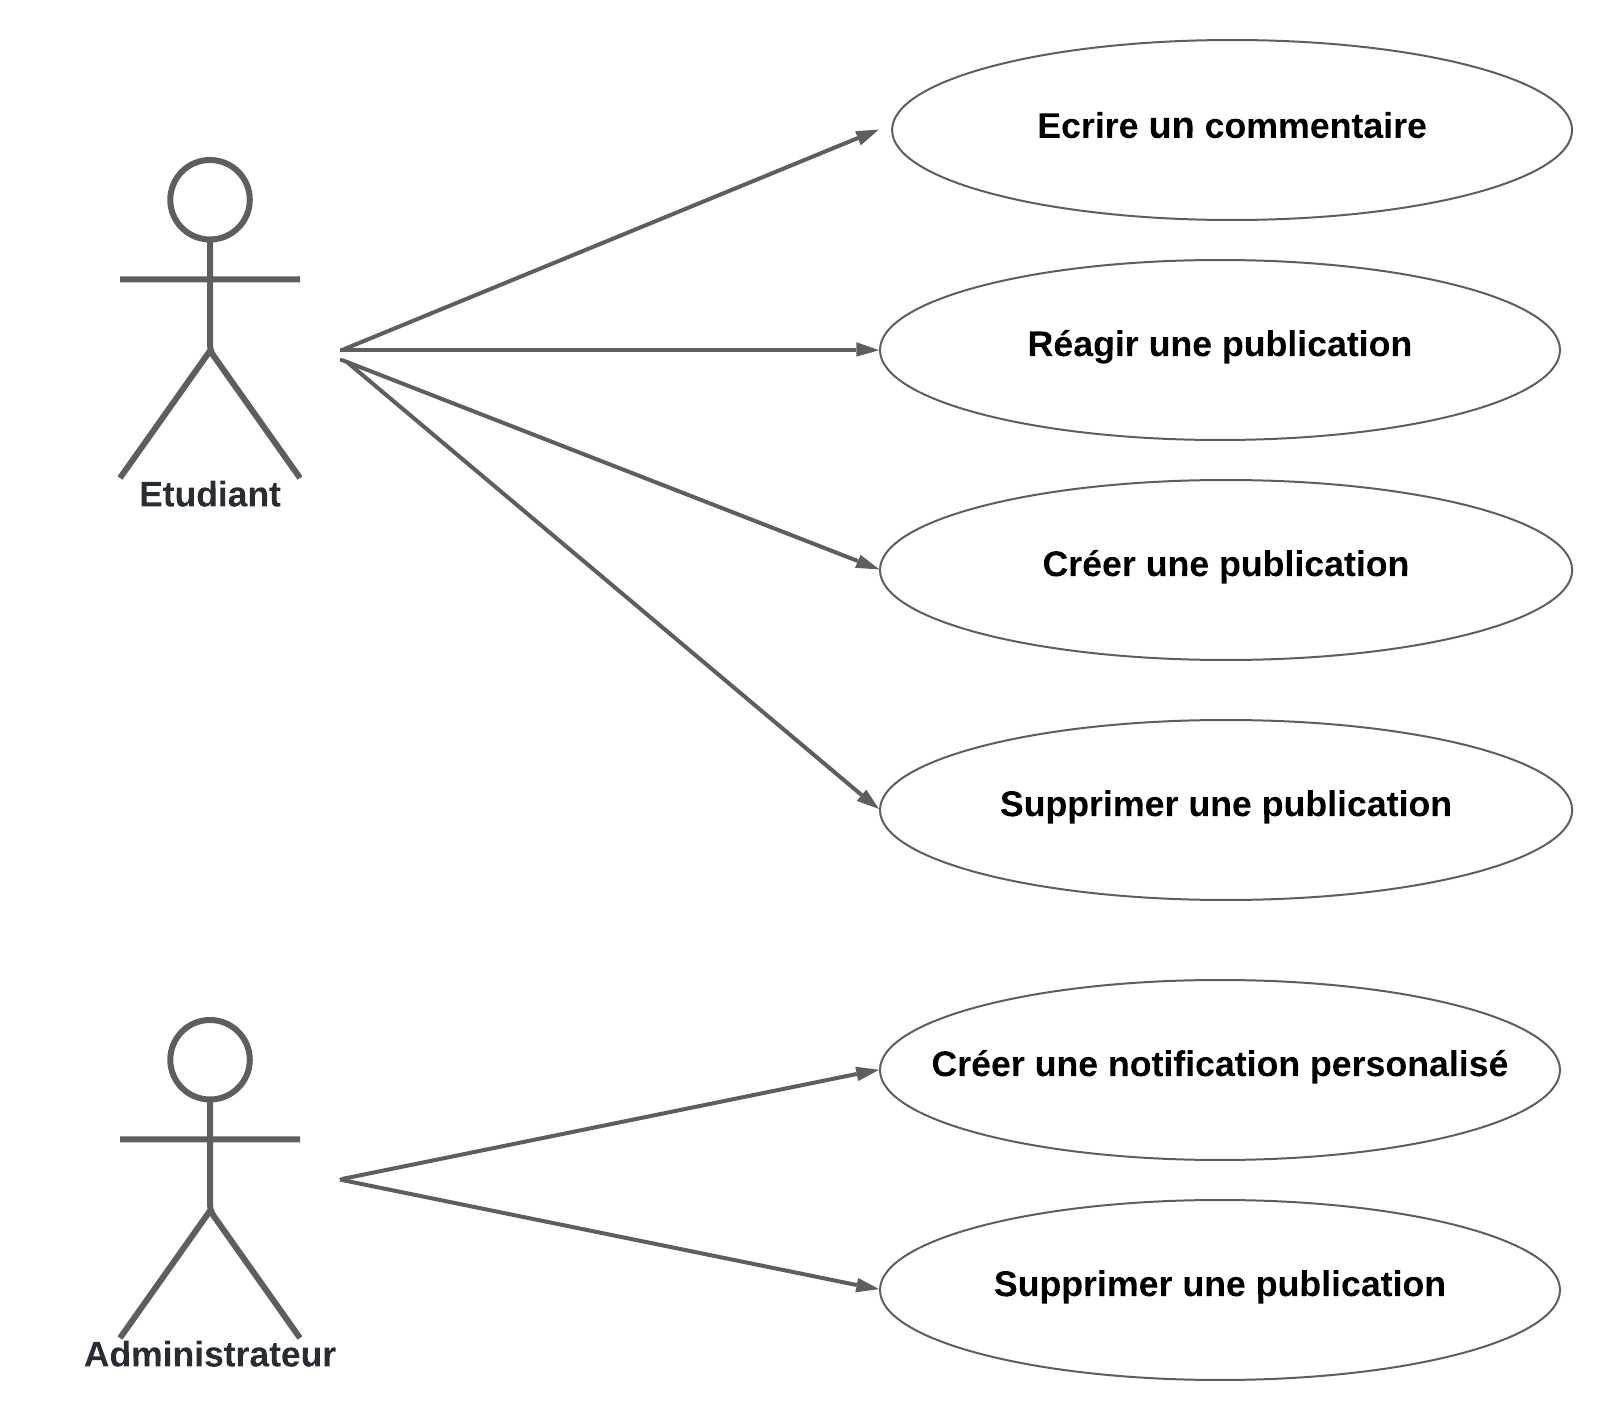
\includegraphics[height=10cm,width=13cm]{images/AAADiagramDesCasPubsNotifs.png}%
    }
    \caption{Diagramme de cas d'utilisation Sprint 4 }
\end{figure}

\vspace{-6mm}
Voici la description mise à jour du cas d'utilisation "Créer une publication" :
\vspace{-9mm}
\subsection{Description textuelle du cas d’utilisation « Créer une publication »}
\vspace{-4mm}
Le tableau ci-dessous détaille le cas d'utilisation "Créer une publication" dans le cadre d'un système où les utilisateurs peuvent publier du contenu après s'être authentifiés.

\begin{table}[h]
\centering
\begin{tabular}{|p{3cm}|p{11cm}|}
\hline
\textbf{Cas d'utilisation } & Créer une publication \\
\hline
\textbf{Acteurs} & Utilisateur \\
\hline
\textbf{Précondition} & Utilisateur authentifié \\
\hline
\textbf{Postcondition} & Publication créée \\
\hline
\textbf{Scénario nominal} & 
\begin{enumerate}
    \item L'utilisateur est sur la page d'accueil.
    \item L'utilisateur clique sur le bouton « Créer une publication ».
    \item Le système affiche le formulaire de création de publication.
    \item L'utilisateur rédige sa publication.
    \item L'utilisateur clique sur le bouton "Publier".
\end{enumerate} \\
\hline
\textbf{Exception} & 
Un champ au moins doit être rempli dans le formulaire de création de publication. Le système affiche un message d'erreur si aucun champ n'est rempli. \\
\hline
\end{tabular}
\caption{Description du cas d’utilisation « Créer une publication »}
\end{table}
\vspace{-4mm}
Voici la description mise à jour du cas d'utilisation "Créer une notification personnalisée" :
\vspace{-1cm}
\subsection{Description textuelle du cas d’utilisation « Créer une notification personnalisée »}
\vspace{-4mm}
Le tableau ci-dessous détaille le cas d'utilisation "Créer une notification personnalisée" dans le cadre d'un système où les administrateurs peuvent envoyer des notifications personnalisées après s'être authentifiés.

\begin{table}[h]
\centering
\begin{tabular}{|p{3cm}|p{11cm}|}
\hline
\textbf{Cas d'utilisation } & Créer une notification personnalisée \\
\hline
\textbf{Acteurs} & Administrateur \\
\hline
\textbf{Précondition} & Administrateur authentifié \\
\hline
\textbf{Postcondition} & Notification créée et envoyée \\
\hline
\textbf{Scénario nominal} & 
\begin{enumerate}
    \item L'administrateur est sur la page d'accueil du dashboard.
    \item L'administrateur navigue dans le sidebar et clique sur le bouton "Notifications".
    \item Le système affiche le formulaire de création de notification.
    \item L'administrateur remplit les champs nécessaires de la notification.
    \item L'administrateur clique sur le bouton "Envoyer".
\end{enumerate} \\
\hline
\textbf{Exception} & 
Tous les champs du formulaire de création de notification doivent être remplis. Le système affiche un message d'erreur si un champ est laissé vide. \\
\hline
\end{tabular}
\caption{Description du cas d’utilisation « Créer une notification personnalisée »}
\end{table}
\vspace{-1cm}
\section{Diagramme de séquence }
\vspace{-4mm}
Pour mieux visualiser les interactions entre l'utilisateur et le système lors de la création de publications et de notifications, nous avons utilisé des diagrammes de séquence. Ces diagrammes décrivent de manière détaillée les étapes impliquées dans la création de publications par les utilisateurs ainsi que la génération de notifications par l'administrateur.
\vspace{-1.5cm}
\subsection{Diagramme de séquence «Créer une publication»}
\vspace{-4mm}
Le diagramme de séquence "Créer une publication" illustre le flux d'actions entre l'utilisateur et le système lorsqu'il souhaite publier du contenu sur l'application. Ce diagramme détaille les étapes telles que l'ouverture de la page de création de publication, la saisie du contenu, et la publication effective de la publication.
\vspace{-4mm}
\begin{figure}[H]%
    \center%
    \setlength{\fboxsep}{5pt}%
    \setlength{\fboxrule}{0.5pt}%
    \fbox{
    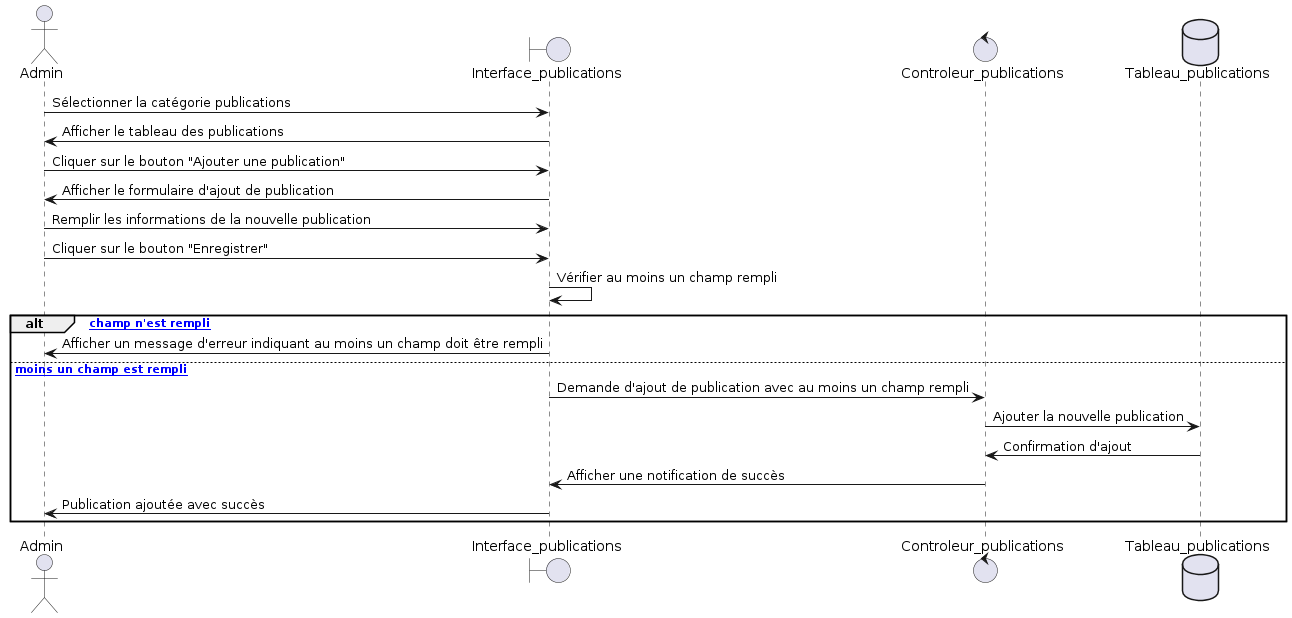
\includegraphics[height=9cm,width=15cm]{images/ffffpublications.png}%
    }
    \caption{Diagramme de séquence créer une publication }
\end{figure}
\vspace{-18mm}
\subsection{Diagramme de séquence «Créer une notification»}
\vspace{-4mm}
Le diagramme de séquence "Créer une notification" montre comment un administrateur crée une notification personnalisée dans le système, ce qui déclenche l'envoi de la notification aux utilisateurs concernés.

\begin{figure}[H]%
    \center%
    \setlength{\fboxsep}{5pt}%
    \setlength{\fboxrule}{0.5pt}%
    \fbox{
    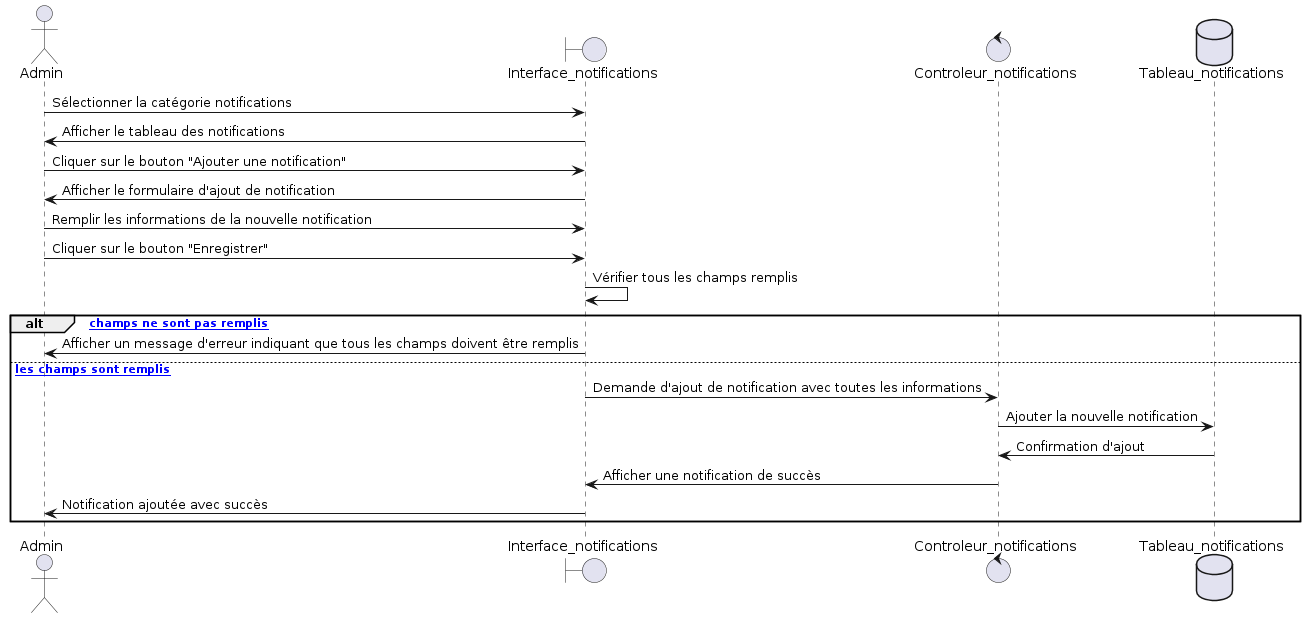
\includegraphics[height=9cm,width=15cm]{images/fffffnotification.png}%
    }
    \caption{Diagramme de séquence «Créer une notification» }
\end{figure}


\section{Diagramme de classes detaillé }
\vspace{-4mm}
Le diagramme de classes présenté ci-dessus illustre la gestion des publications et des notifications dans notre système. 

\begin{figure}[H]%
    \center%
    \setlength{\fboxsep}{5pt}%
    \setlength{\fboxrule}{0.5pt}%
    \fbox{
    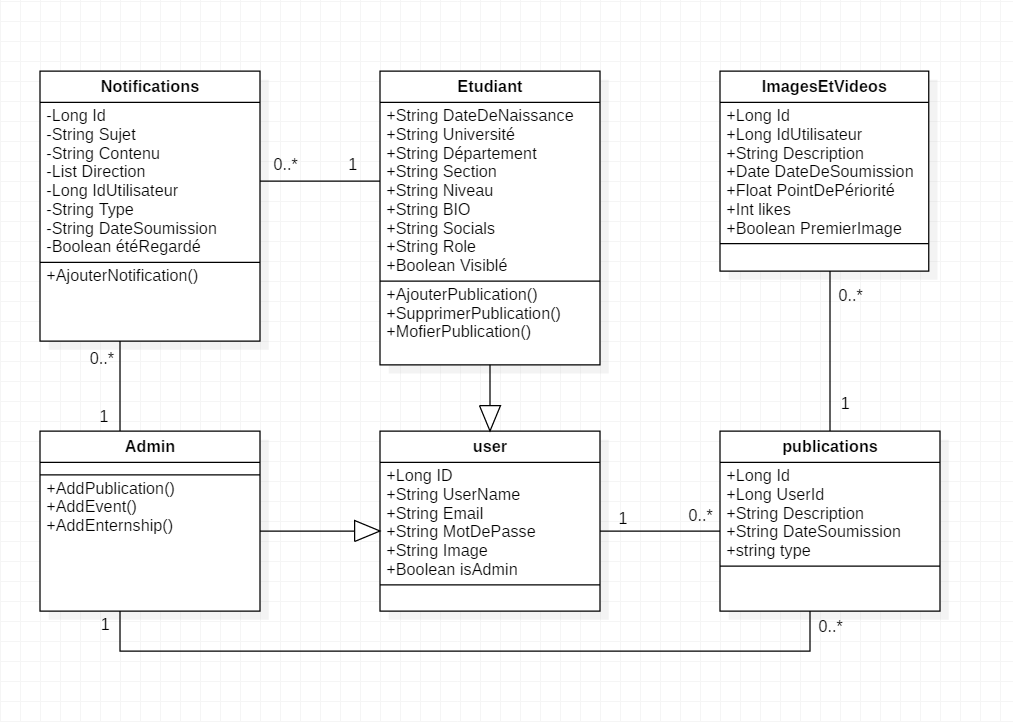
\includegraphics[height=15cm,width=15cm]{images/AAANotificatiosnPubs.png}%
    }
    \caption{Diagramme de classes Sprint 4}
\end{figure}
\vspace{-1cm}

\section{Réalisation }
\vspace{-6mm}
\subsection{Page créer une publication}
\vspace{-4mm}
La page "Créer une publication" dans la partie mobile permet à l'utilisateur de rédiger et de publier du contenu.
\vspace{-4mm}
\begin{figure}[H]%
    \center%
    \setlength{\fboxsep}{5pt}%
    \setlength{\fboxrule}{0.5pt}%
    \fbox{
    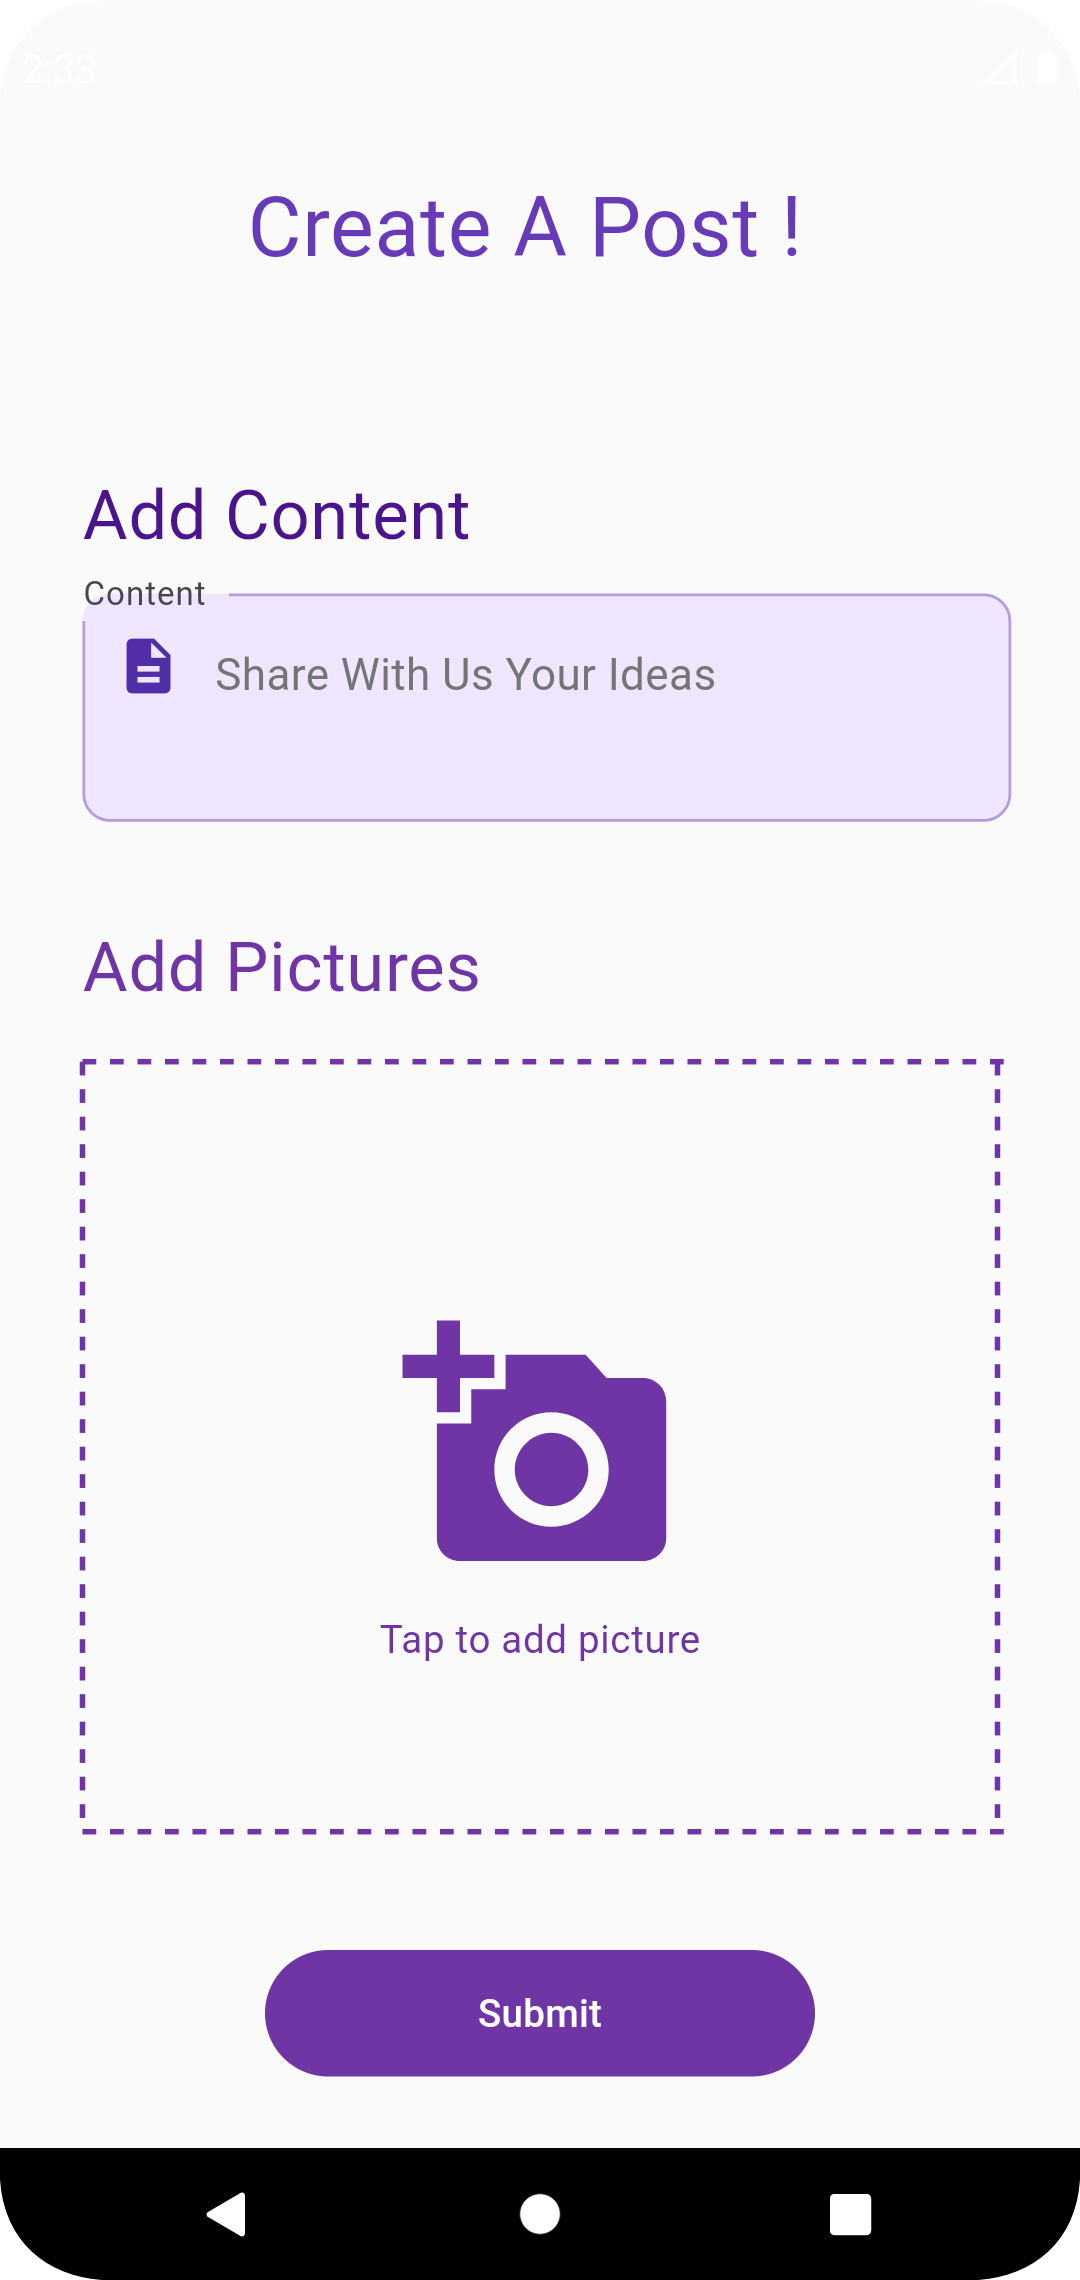
\includegraphics[height=9.8cm,width=7cm]{images/AddPostPage.png}%
    }
    \caption{Interface créer une publication}
\end{figure}
\vspace{-1.8cm}
\section{Interface commenter et réagir sur une publication}
\vspace{-8mm}
Les utilisateurs peuvent commenter ou réagir aux publications avant même de consulter les commentaires et réactions des autres utilisateurs.
\begin{figure}[H]%
    \center%
    \setlength{\fboxsep}{5pt}%
    \setlength{\fboxrule}{0.5pt}%
    \fbox{
    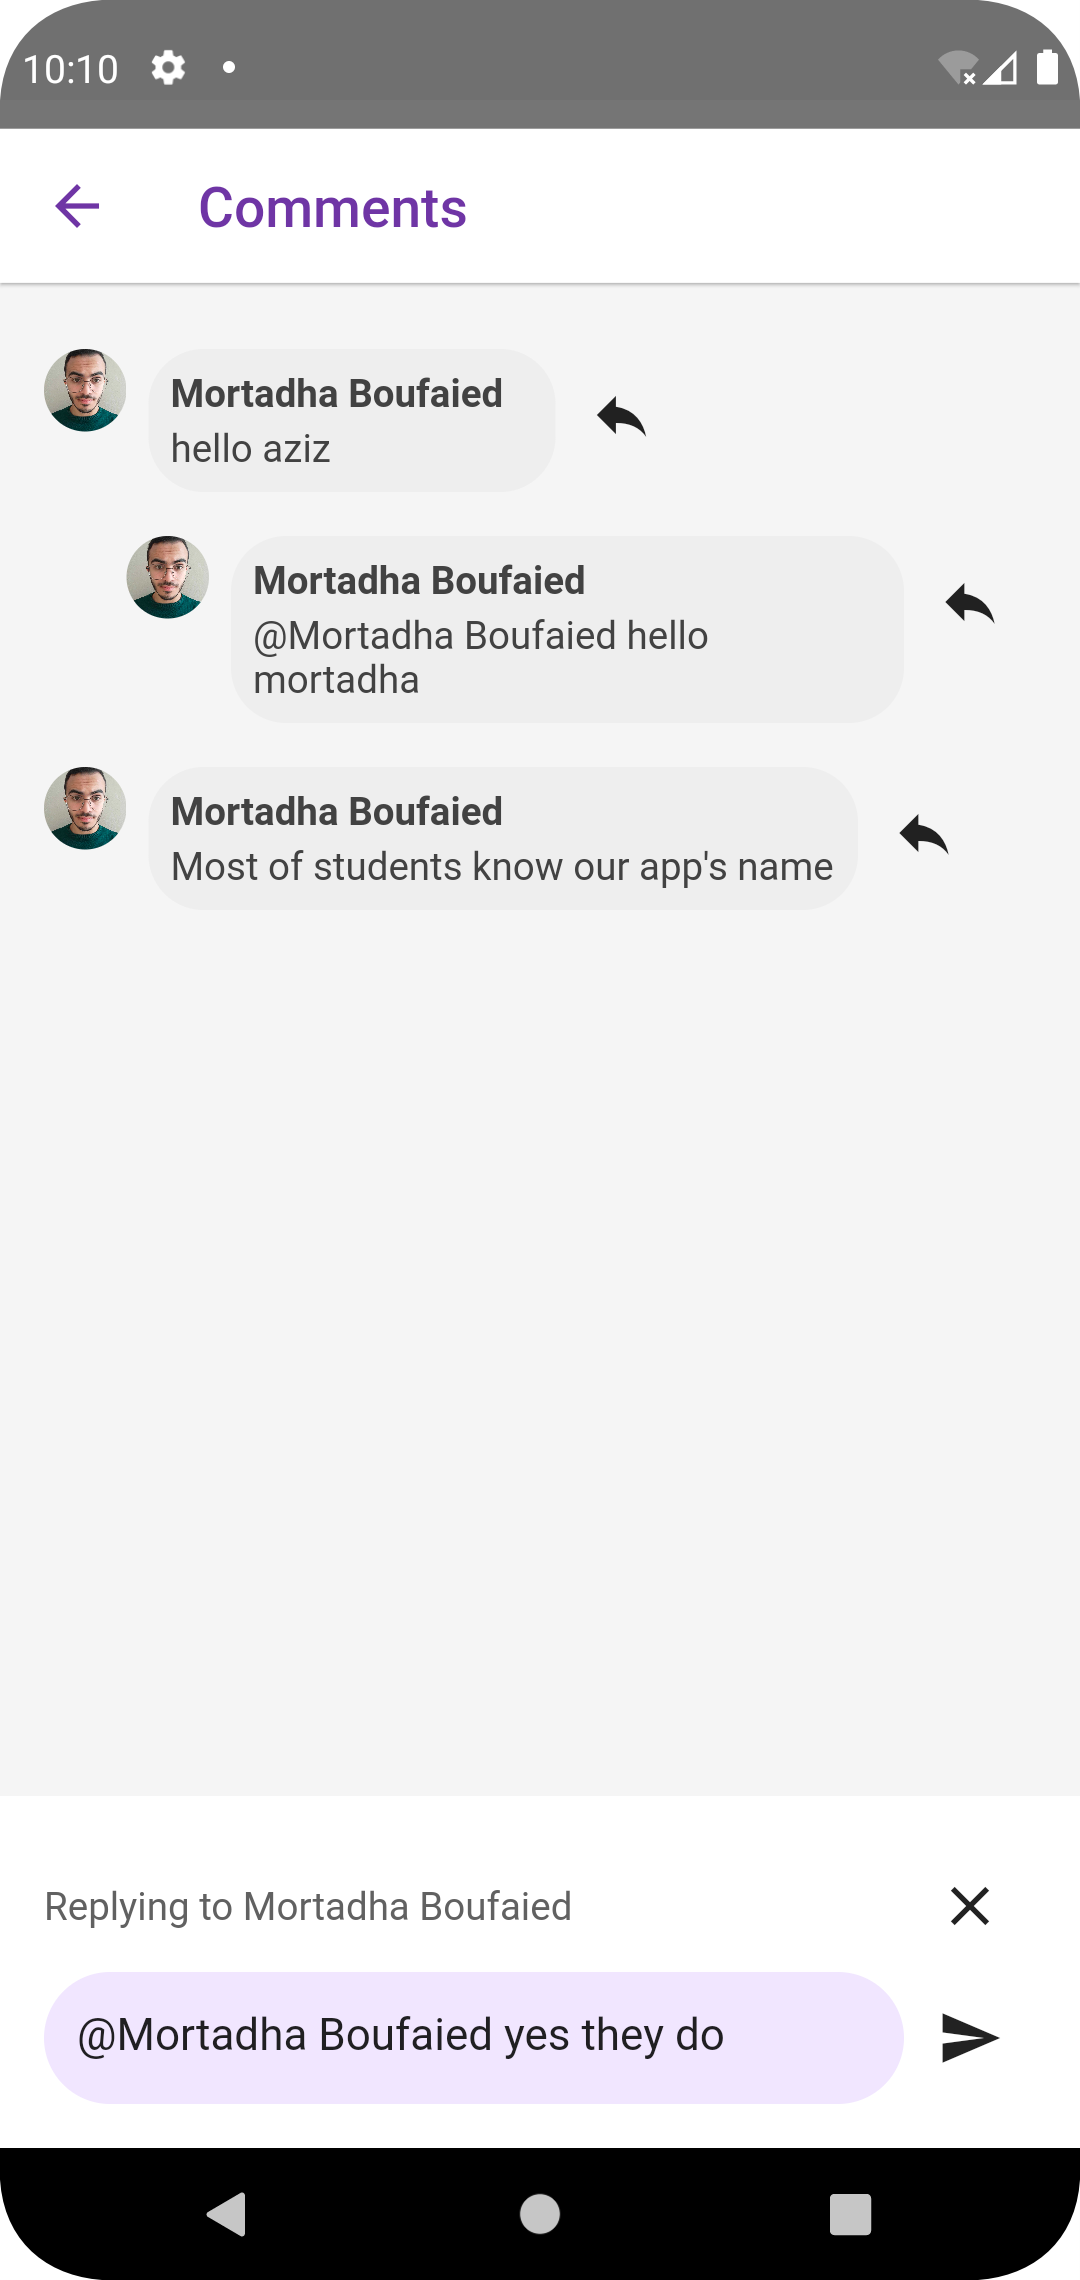
\includegraphics[height=9.8cm,width=7cm]{images/XCommentsBar.png}%
    }
    \caption{Interface ajout d'un commentaire }
\end{figure}

\vspace{-10mm}
\subsection{Interface Acceuil mobile }
\vspace{-7mm}
Sur la page d'accueil de l'application mobile, toutes les publications sont visibles.
\vspace{-2mm}
\begin{figure}[H]%
    \center%
    \setlength{\fboxsep}{5pt}%
    \setlength{\fboxrule}{0.5pt}%
    \fbox{
    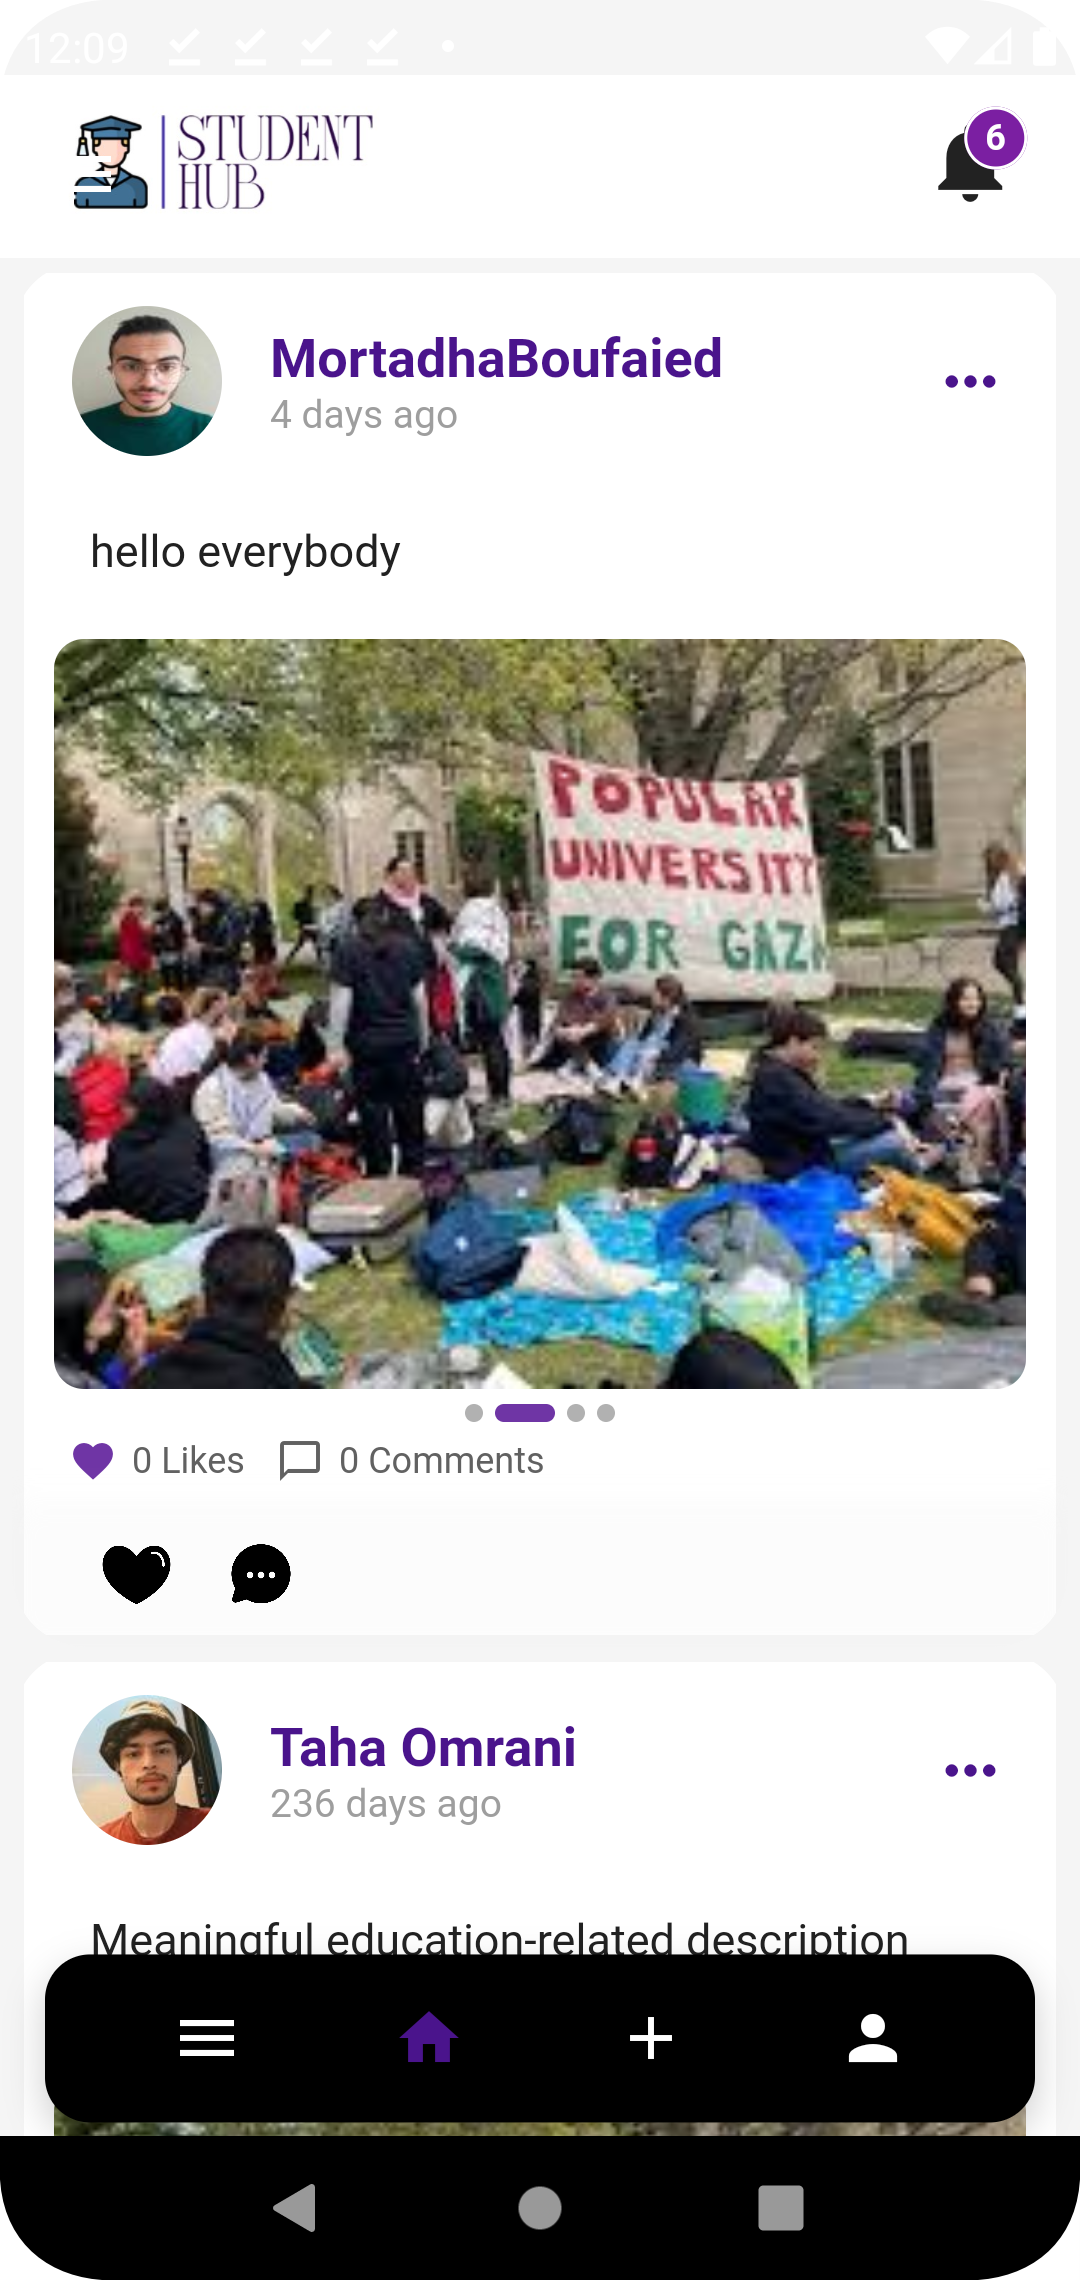
\includegraphics[height=9.5cm,width=7cm]{images/AAAHomePage.png}%
    }
    \caption{Interface page d'accueil partie mobile}
\end{figure}

\vspace{-1.8cm}
\subsection{Interface Notification mobile }
\vspace{-7mm}
La page de notifications affiche les notifications reçues par l'utilisateur.
\vspace{-2mm}
\begin{figure}[H]%
    \center%
    \setlength{\fboxsep}{5pt}%
    \setlength{\fboxrule}{0.5pt}%
    \fbox{
    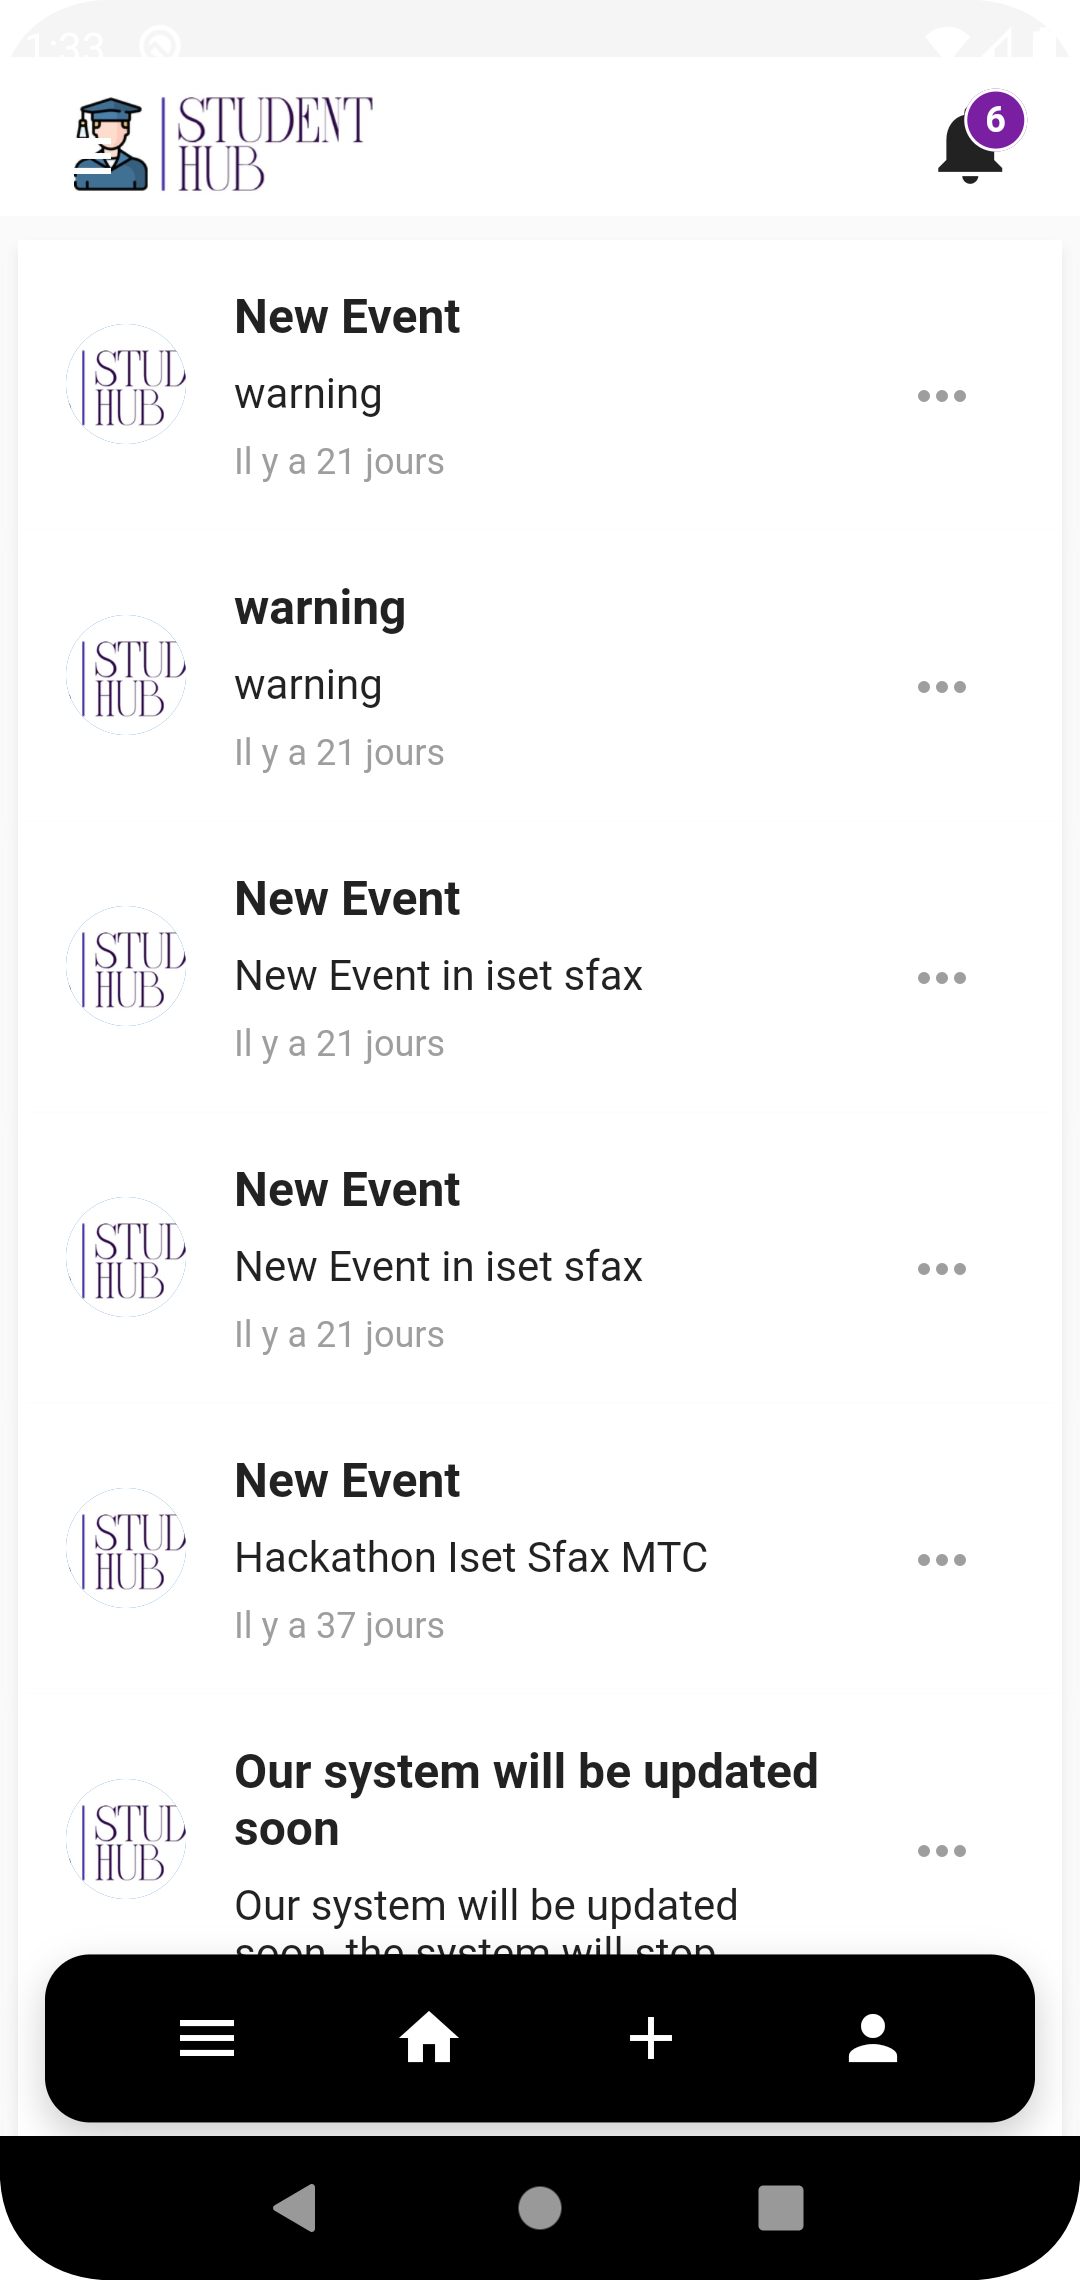
\includegraphics[height=9.5cm,width=7cm]{images/AAANotifications.png}%
    }
    \caption{Interface Notification Partie Mobile}
\end{figure}

\subsection{Interface Notification Personalisée  }
\vspace{-4mm}
L'interface web pour l'administrateur permet de créer des notifications personnalisées. Depuis le tableau de bord, l'administrateur peut accéder à un formulaire pour rédiger le contenu de la notification. Une fois la notification créée et envoyée, elle est visible pour les utilisateurs de l'application mobile, garantissant que les messages importants et spécifiques atteignent rapidement les utilisateurs.

\begin{figure}[H]%
    \center%
    \setlength{\fboxsep}{5pt}%
    \setlength{\fboxrule}{0.5pt}%
    \fbox{
    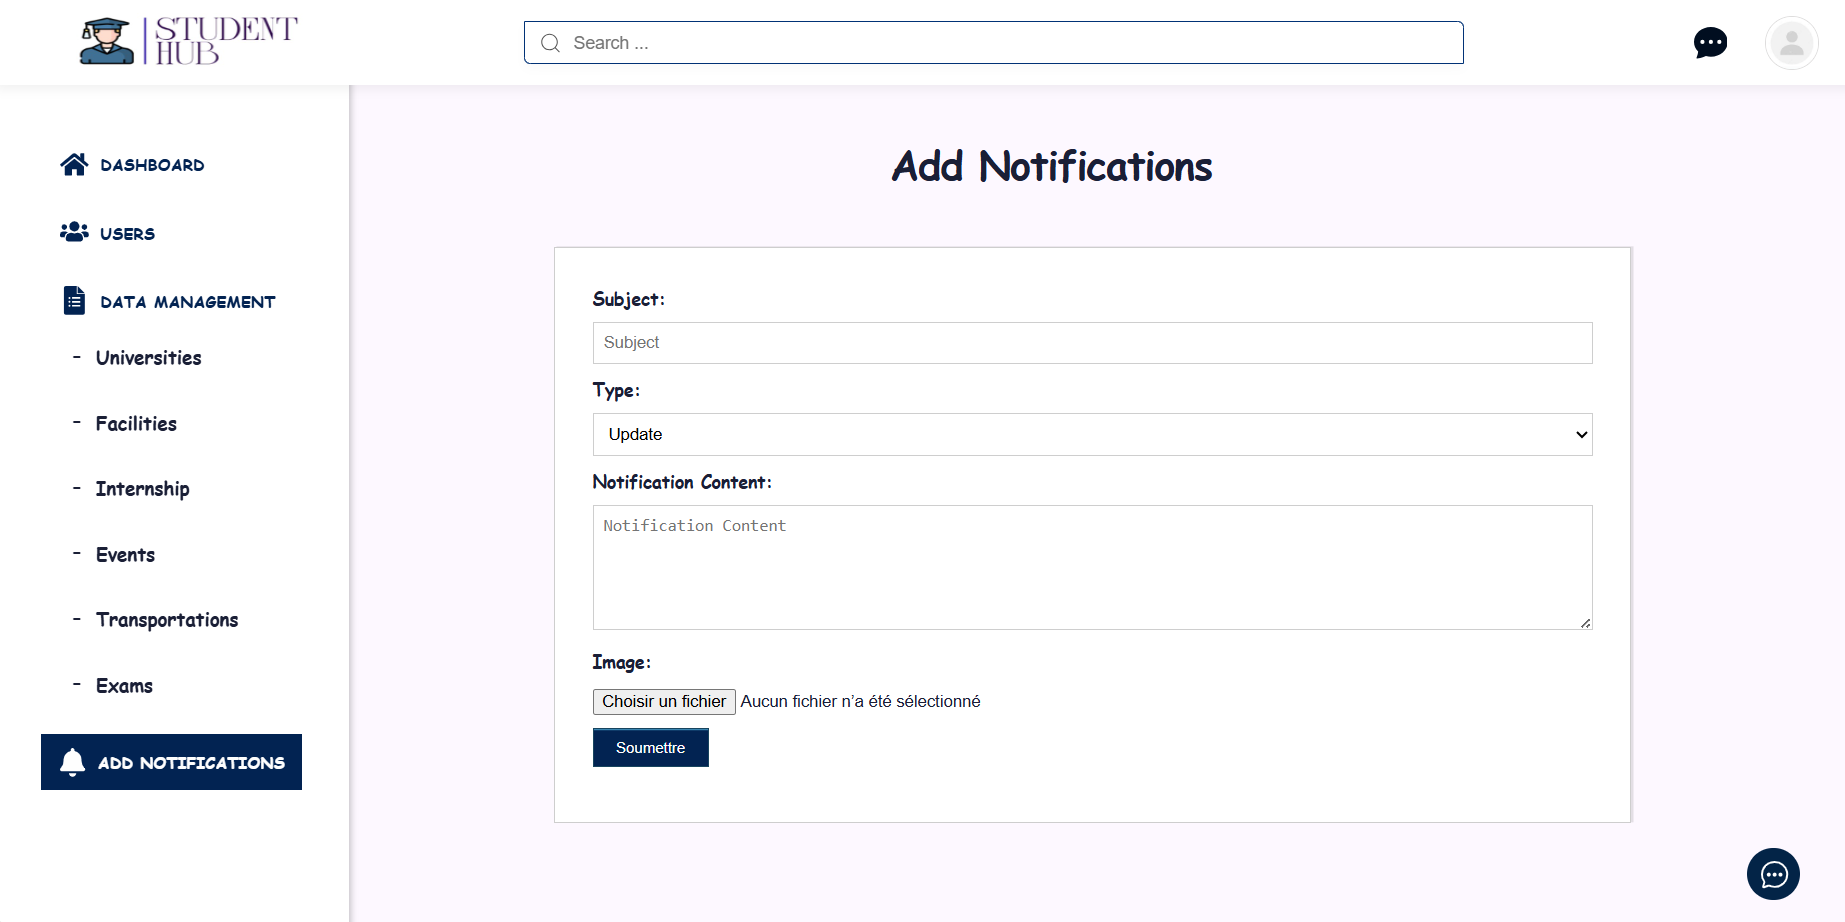
\includegraphics[height=10cm,width=15.5cm]{images/AAAAddNotifications.png}%
    }
    \caption{Interface Notification personalisée }
\end{figure}

\vspace{-1.5cm}
\subsection{Conclusion }
\vspace{-4mm}
En conclusion de ce sprint, nous avons mis en place un système de chat entre l'administration et les étudiants, ainsi qu'un tableau de bord affichant des graphiques pertinents dans la partie web admin. De plus, nous avons introduit une carte interactive pour guider les étudiants et les informer sur leur environnement. Ces ajouts renforcent notre engagement à améliorer l'expérience utilisateur.

\end{sloppypar} 

    \chapter{ Chapitre 8 : Sprint 5 "Recherche des données sur un Map, \centering Gestion des tableaux de bord et des Messageries"}
\begin{spacing}{1.2}
\minitoc
\thispagestyle{MyStyle}
\end{spacing}
\newpage
\begin{sloppypar} 

\section{Introduction}
\vspace{-4mm}
Dans ce sprint, nous améliorons la communication entre l'administration et les étudiants via un chat dashboard dans la partie web admin. De plus, nous ajoutons une carte interactive pour guider les étudiants. Ces améliorations visent à faciliter la communication et à offrir une expérience utilisateur plus intuitive. 
\vspace{-8mm}

\section{Backlog du sprint}
\vspace{-4mm}
Le backlog pour le chat, le tableau de bord et la carte inclut des fonctionnalités telles que la mise en place d'un système de messagerie instantanée entre l'administrateur et les utilisateurs, le développement d'un tableau de bord pour afficher des données clés et la création d'une carte interactive pour aider les utilisateurs à naviguer et à trouver des informations pertinentes. Ces fonctionnalités visent à améliorer l'expérience utilisateur et à fournir des outils efficaces pour la gestion et la visualisation des données.

\begin{table}[h]
\centering
\begin{tabular}{|p{9cm}|p{3cm}|p{3cm}|}
\hline
\textbf{ Tâches } & \textbf{ Priorité }& \textbf{Période/jour}  \\
\hline
En tant qu’un étudiant ,je peux contacter l’administrateur.& Élevée  & 5 jours \\
\hline
En tant qu'un étudiant , je peux contacter l’administrateur sur l'application mobile.  & Élevée  & 4 jours  \\
\hline
En tant qu’un administrateur, je peux consulter le tableau de bord dans l’application web & Élevée  & 7 jours  \\
\hline
En tant qu’un utilisateur ,je peux consulter la carte map sur l'application mobile  & Élevée  & 7 jours  \\
\hline

\end{tabular}
\caption{Tableau de Backlog de produit Sprint 5}
\end{table}
\vspace{-1cm}
\section {Analyse et spécification des besoins}
\vspace{-4mm}
Afin de mieux comprendre la structure de notre système, nous avons utilisé un diagramme de cas d'utilisations qui est présenté ci-dessous.
\vspace{-5mm}
\subsection{Diagramme de cas d’utilisation détaillé}
\vspace{-4mm}
Ce diagramme de cas d'utilisation illustre un système de communication entre étudiants et administrateurs, décrivant deux interactions principales :

\begin{figure}[H]%
    \center%
    \setlength{\fboxsep}{5pt}%
    \setlength{\fboxrule}{0.5pt}%
    \fbox{
    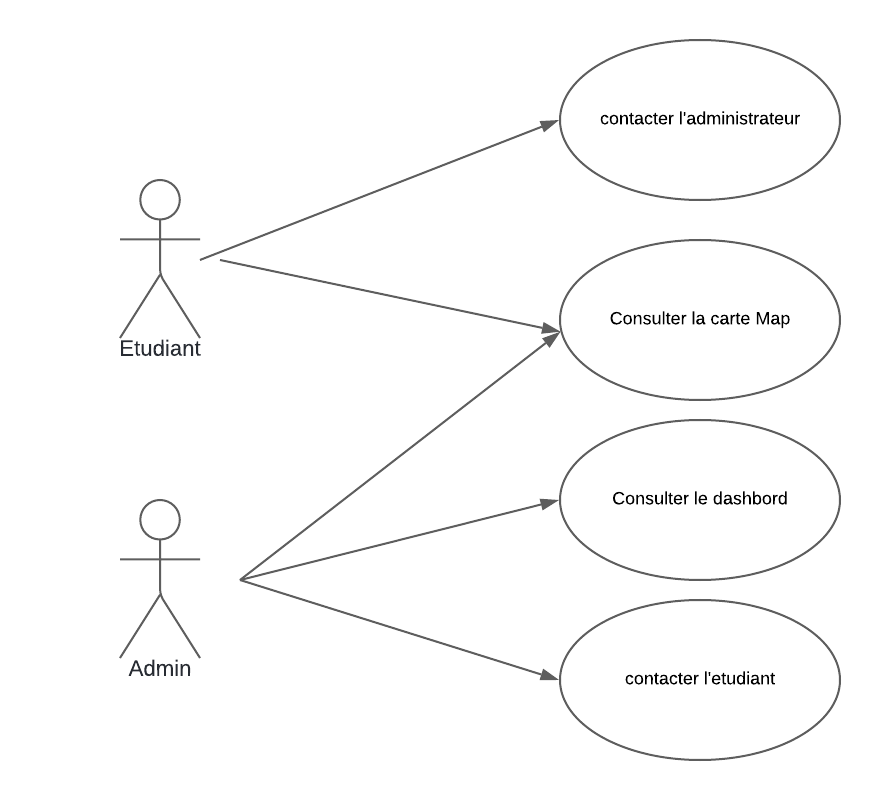
\includegraphics[height=6cm,width=12cm]{images/diagramme de cas d'utilisation 5eme sprint.png}%
    }
    \caption{Diagramme de cas d'utilisation Sprint 5 }
\end{figure}
\vspace{-9mm}
\subsection{Description textuelle du cas d’utilisation «Envoyer un message à l'administrateur»}
\vspace{-4mm}
Le tableau ci-dessous détaille le cas d'utilisation "Envoyer un message à l’administrateur" dans le cadre d'un système où les étudiants peuvent contacter l'administrateur après s'être connectés.

\begin{table}[h]
\centering
\begin{tabular}{|p{3cm}|p{12cm}|}
\hline
\textbf{Cas d'utilisation } & Envoyer un message à l'administrateur \\
\hline
\textbf{Acteurs} & Étudiant \\
\hline
\textbf{Précondition} & Utilisateur connecté \\
\hline
\textbf{Postcondition} & Message envoyé à l'administrateur \\
\hline
\textbf{Scénario nominal} & 
\begin{enumerate}
    \item L'Étudiant est sur la page d'accueil.
    \item L'Étudiant clique sur le bouton « Contact ».
    \item Le système affiche le formulaire d'envoi de message à l'administrateur.
    \item L'Étudiant rédige son message.
    \item L'Étudiant envoie le message.
\end{enumerate} \\
\hline
\end{tabular}
\caption{Description du cas d’utilisation « Envoyer un message à l'administrateur »}
\end{table}
\vspace{-9mm}
\subsection{Description textuelle du cas d’utilisation «Envoyer un message à un Étudiant»}
\vspace{-4mm}
Le tableau ci-dessous détaille le cas d'utilisation "Envoyer un message à un Étudiant" dans un système où les administrateurs peuvent contacter des étudiants spécifiques après s'être authentifiés.
\vspace{-3mm}
\begin{table}[h]
\centering
\begin{tabular}{|p{3cm}|p{12cm}|}
\hline
\textbf{Cas d'utilisation } & Envoyer un message  \\
\hline
\textbf{Acteurs} &  Admin \\
\hline
\textbf{Précondition} & Admin authentifié \\
\hline
\textbf{Postcondition} &   Étudiant connecté\\
\hline
\textbf{Scénario nominal} &
\begin{enumerate}
   \item L'administrateur est sur la page Dashboard.
    \item L'administrateur clique sur le bouton "Contacter".
    \item L'administrateur choisit l'étudiant à contacter..
    \item Le système affiche le formulaire d'envoi de message à l'administrateur.
    \item L'administrateur rédige son message.
    \item L'administrateur envoie le message.
\end{enumerate} \\
\hline
\end{tabular}
\caption{Description du cas d’utilisation «Envoyer un message à un Étudiant »}
\end{table}
\vspace{-1.9cm}
\section{Diagramme de séquence }
\vspace{-4mm}
Les diagrammes de séquence pour ce sprint se concentrent sur la fonctionnalité de chat, illustrant le processus par lequel les utilisateurs peuvent échanger des messages en temps réel avec d'autres utilisateurs ou avec l'administrateur de l'application, facilitant ainsi la communication et la résolution des problèmes de manière efficace.
\vspace{-1cm}
\subsection{Diagramme  de séquence <<Contacter un étudiant>> }

\vspace{-4mm}

Le diagramme de séquence "Contacter un étudiant" présente le processus par lequel un administrateur peut contacter un étudiant via l'application web, en initiant une interaction qui permet d'envoyer un message direct à un étudiant spécifique.

\begin{figure}[H]%
    \center%
    \setlength{\fboxsep}{5pt}%
    \setlength{\fboxrule}{0.5pt}%
    \fbox{
    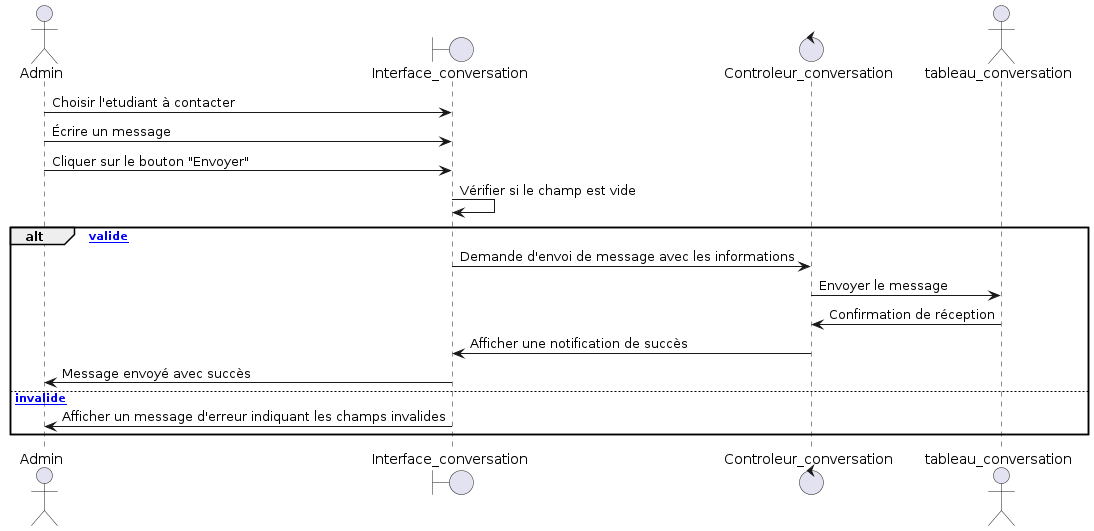
\includegraphics[height=7cm,width=15cm]{images/admintoetudiant.png}%
    }
    \caption{Diagramme de cas d'utilisation }
\end{figure}
\vspace{-4mm}
\subsection{Diagramme de séquence <<Contacter admin>> }
\vspace{-4mm}
Le diagramme de séquence "Contacter l'administrateur" illustre le processus par lequel un utilisateur peut contacter l'administrateur de l'application via l'interface de communication dédiée, permettant ainsi d'envoyer un message direct à l'administrateur pour poser des questions, signaler des problèmes ou demander de l'aide.

\begin{figure}[H]%
    \center%
    \setlength{\fboxsep}{5pt}%
    \setlength{\fboxrule}{0.5pt}%
    \fbox{
    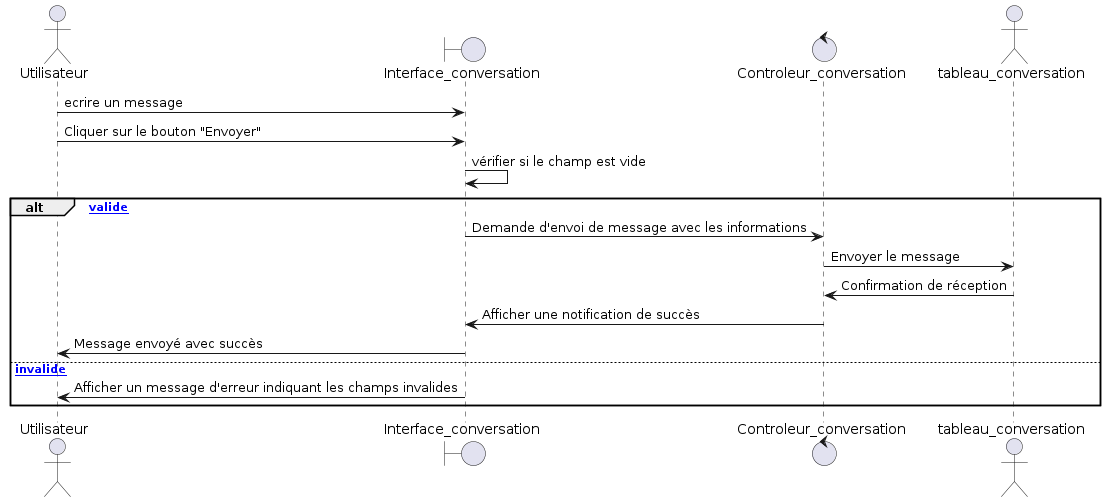
\includegraphics[height=12cm,width=15cm]{images/lasstcontact.png}%
    }
    \caption{Diagramme de séquence <<Contacter admin>> }
\end{figure}


\vspace{-9mm}


\section{Diagramme de classes }
\vspace{-4mm}
Le diagramme de classes pour la gestion de la carte, du chat et du tableau de bord dans notre système offre une représentation structurée des entités et des fonctionnalités associées. Chaque classe, comme "Carte", "Chat" et "Tableau de bord", est conçue pour gérer les opérations spécifiques liées à sa fonctionnalité respective. 
\vspace{-4mm}
\begin{figure}[H]%
    \center%
    \setlength{\fboxsep}{5pt}%
    \setlength{\fboxrule}{0.5pt}%
    \fbox{
    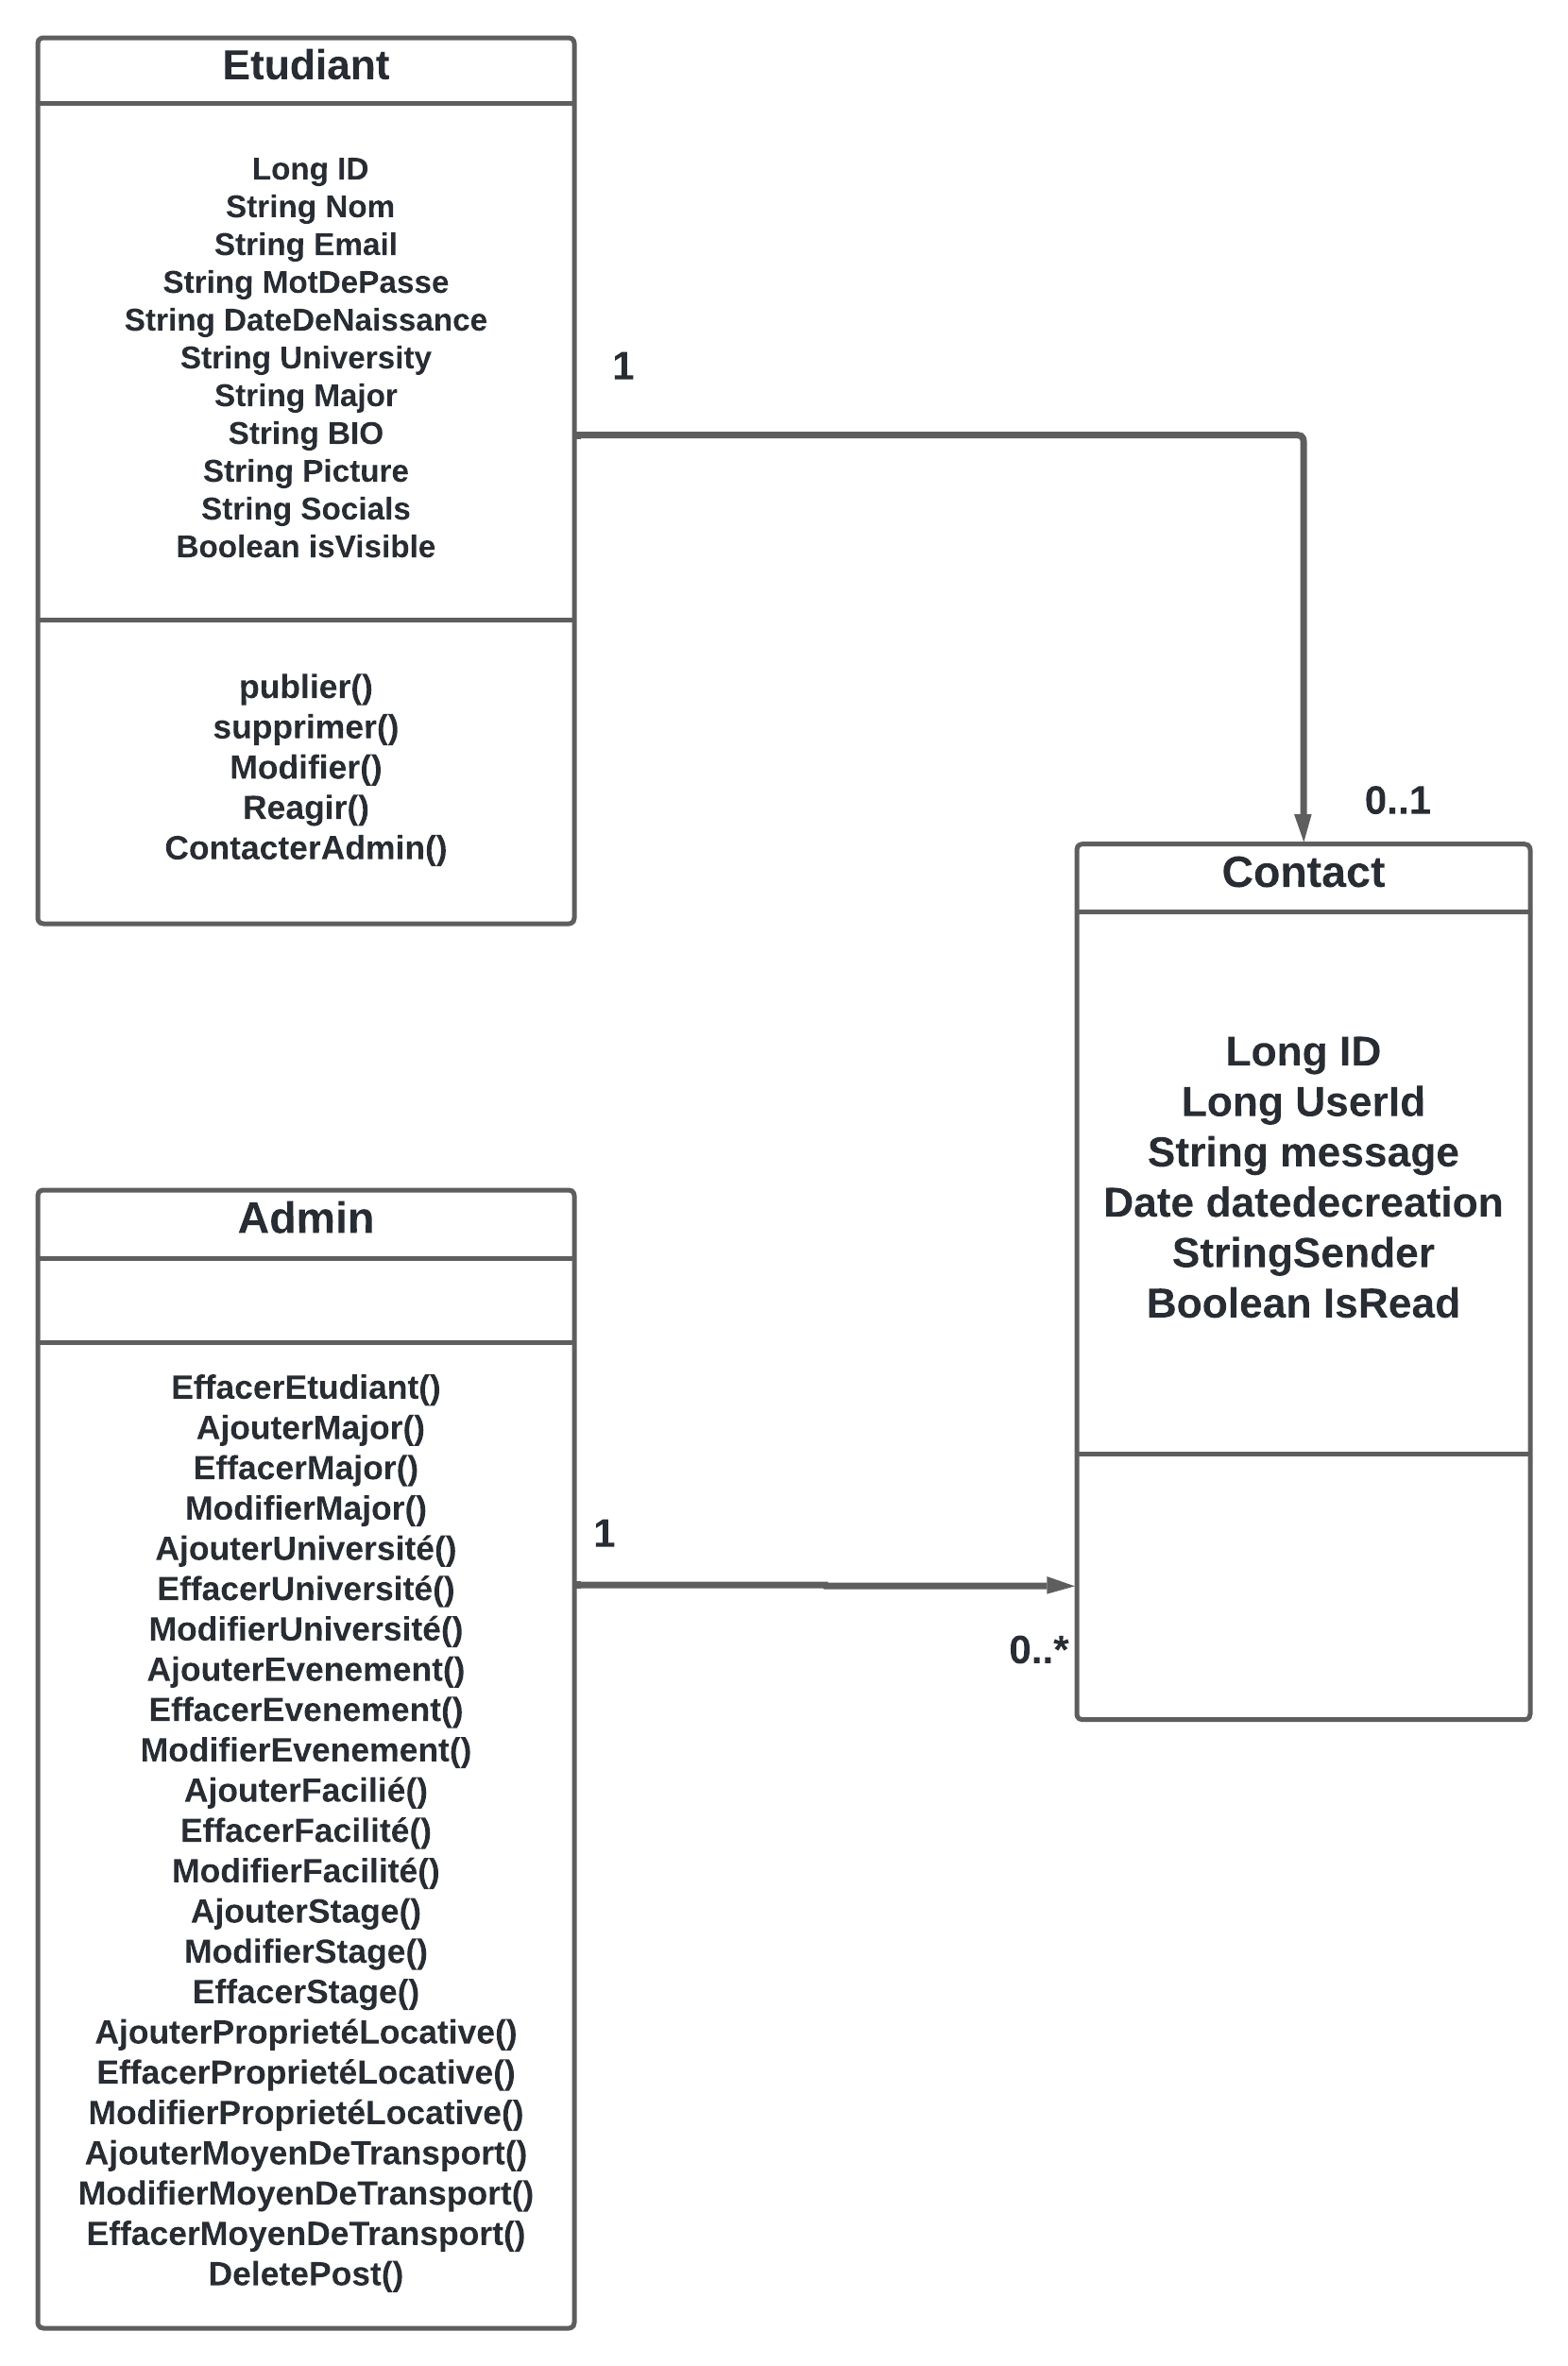
\includegraphics[height=13cm,width=15cm]{images/Diagramme de classe contact (2).png}%
    }
    \caption{Diagramme de classes sprint 5 }
\end{figure}
\vspace{-1.2cm}
\section{Réalisation }
\vspace{-4mm}
La partie de réalisation représente la dernière phase du cycle de développement d’un sprint. Elle permet de présenter les résultats obtenus lors de l’étape de développement afin d’assurer et de garantir une version de qualité. Nous allons montrer cela par des captures d’écrans des fonctionnalités ayant été développées.
\vspace{-1cm}
\section{Contact administrateur}
\vspace{-4mm}
L'interface "Contacter l'administrateur" dans la partie mobile permet aux utilisateurs d'envoyer des messages directement à l'administrateur. Les utilisateurs peuvent rédiger leur message et l'envoyer en un clic, facilitant ainsi une communication directe et efficace avec l'administration.
\vspace{-4mm}
\begin{figure}[H]%
    \center%
    \setlength{\fboxsep}{5pt}%
    \setlength{\fboxrule}{0.5pt}%
    \fbox{
    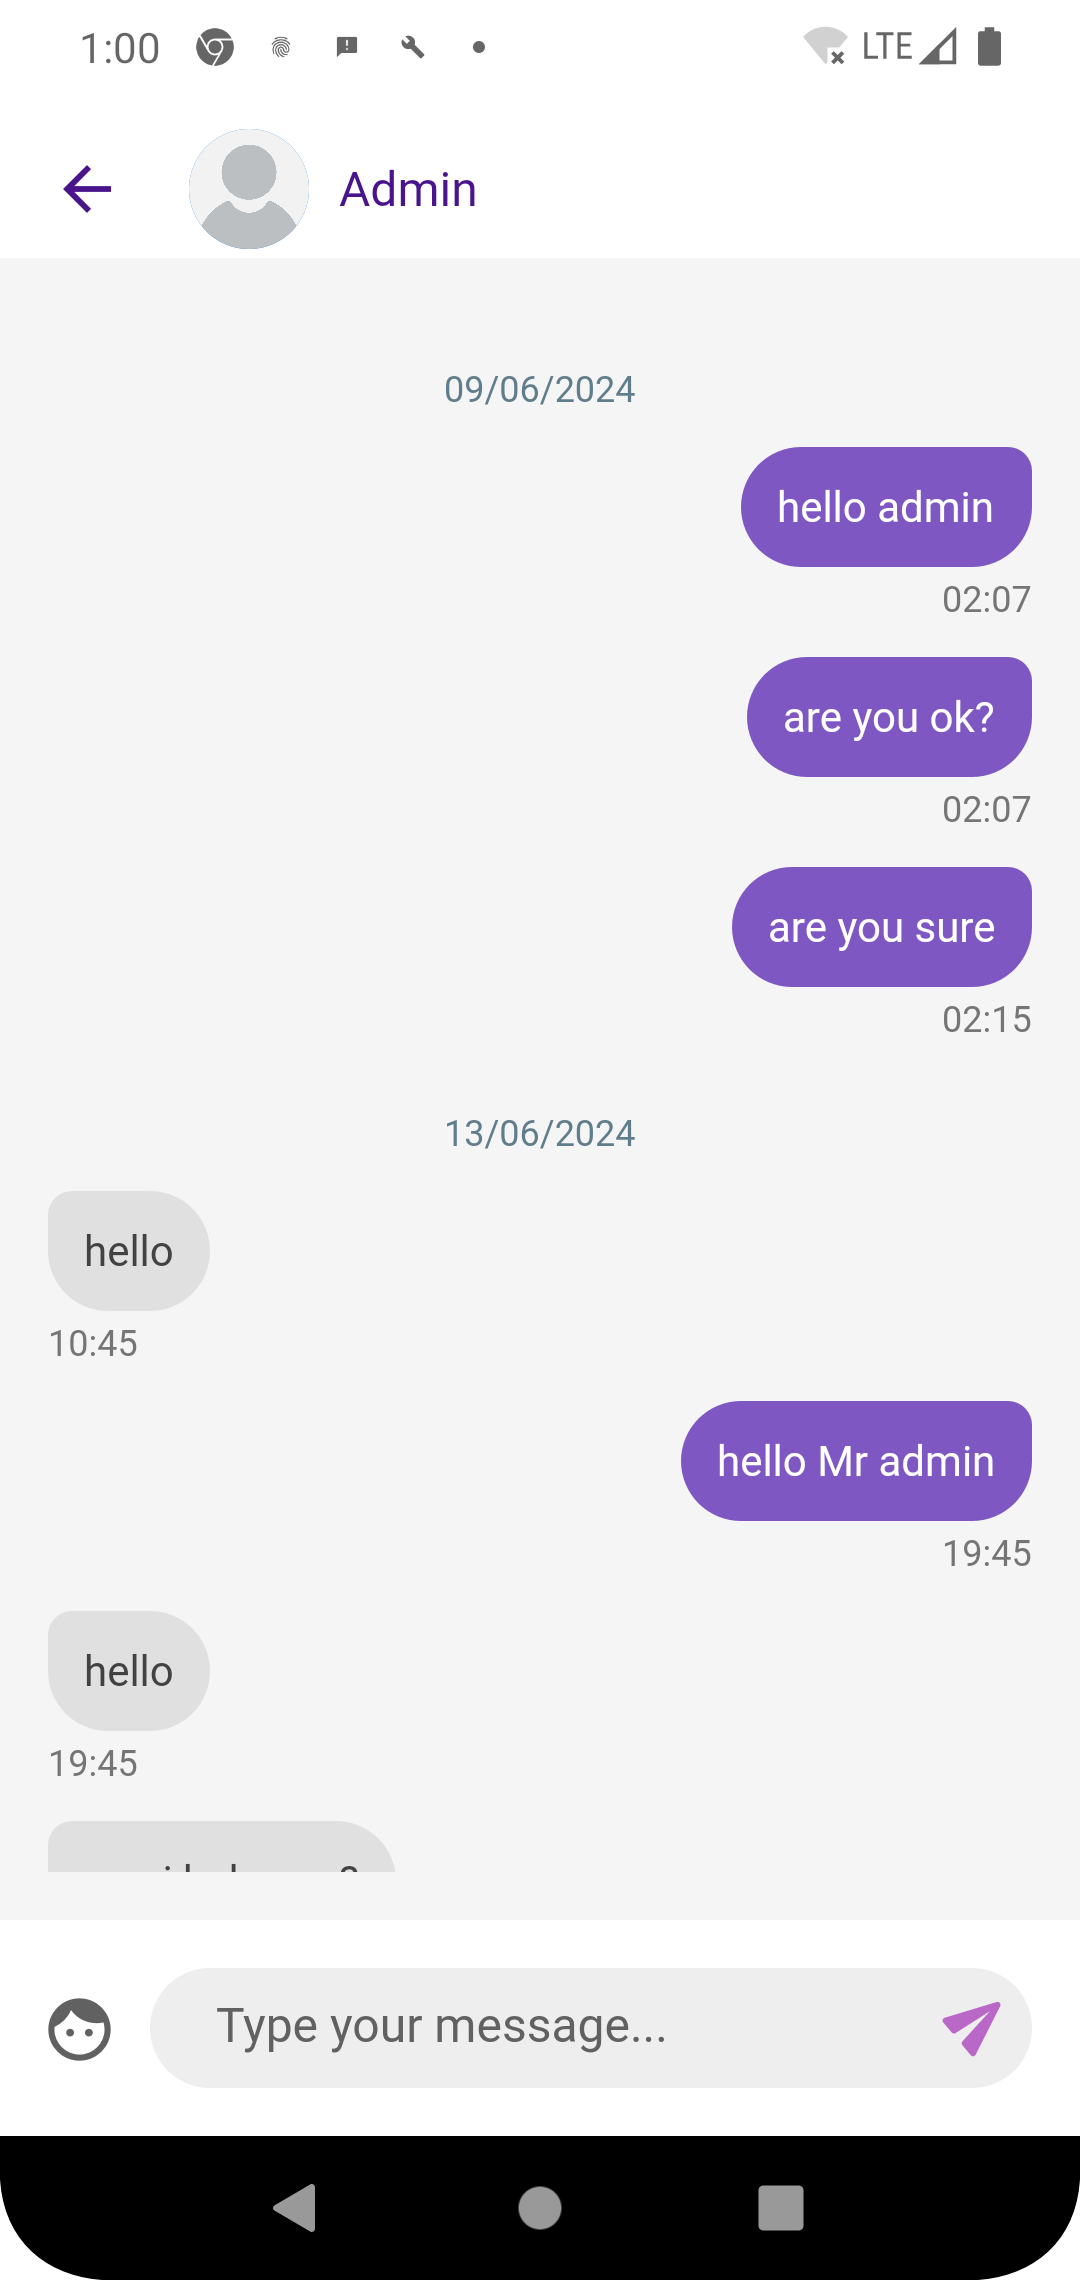
\includegraphics[height=10cm,width=7cm]{images/XChatPage.png}%
    }
    \caption{Interface Contacter administrateur  }
\end{figure}
\vspace{-1.5cm}
\section{Contact Utilisateur }
\vspace{-4mm}
L'interface web pour l'administrateur facilite la communication avec les utilisateurs. Elle offre une section dédiée où l'administrateur peut sélectionner des utilisateurs spécifiques, rédiger un message, et l'envoyer directement, assurant ainsi une communication efficace et directe.

\begin{figure}[H]%
    \center%
    \setlength{\fboxsep}{5pt}%
    \setlength{\fboxrule}{0.5pt}%
    \fbox{
    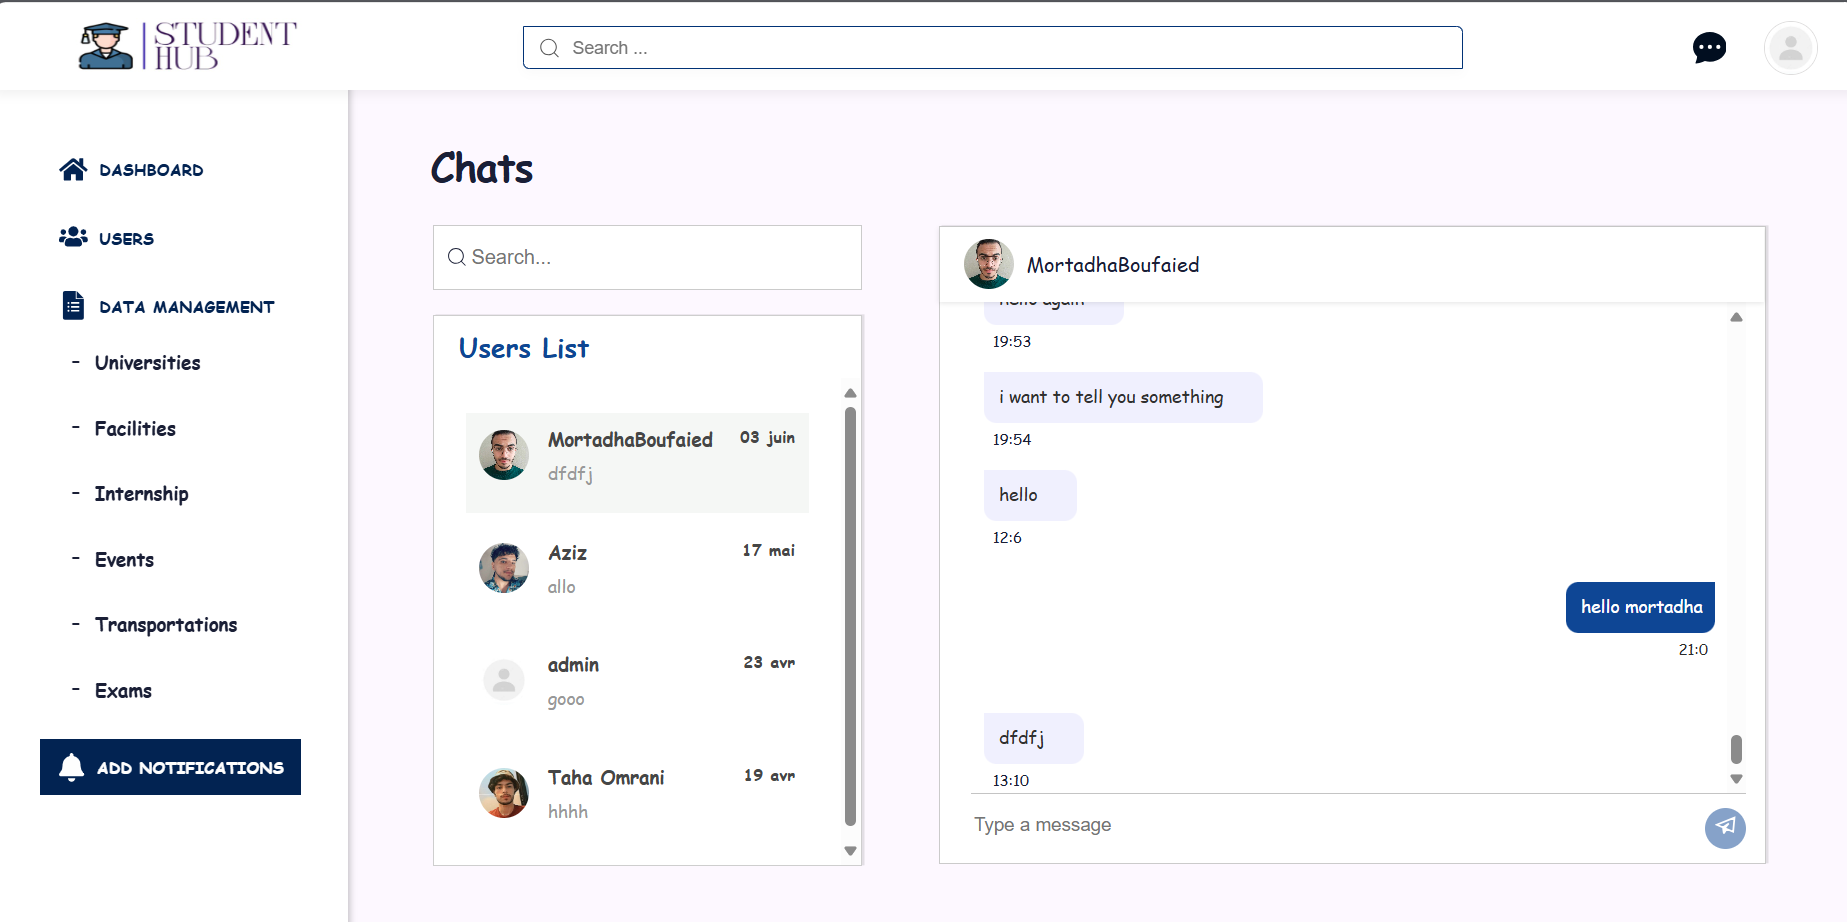
\includegraphics[height=8cm,width=15.5cm]{images/AAAChat.png}%
    }
\end{figure}
\vspace{-7mm}
\vspace{-4mm}
\begin{figure}[H]%
    \center%
    \setlength{\fboxsep}{5pt}%
    \setlength{\fboxrule}{0.5pt}%
    \fbox{
    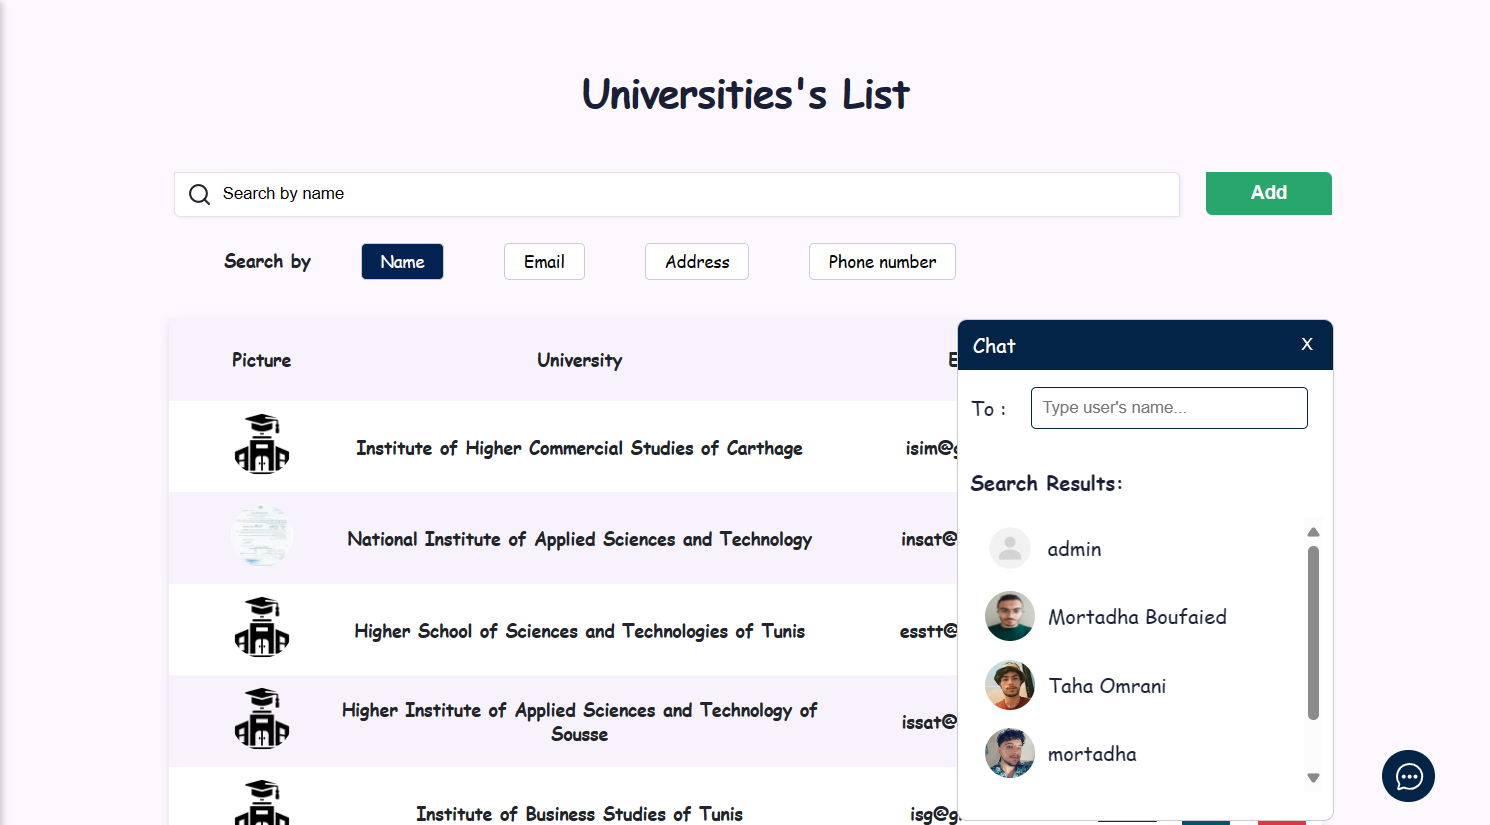
\includegraphics[height=8cm,width=15.5cm]{images/MiniChat.png}%
    }
    \caption{Interface Contacter un utilisateur  }
\end{figure}

\vspace{-1.2cm}

\section{Le Dashbord d'administrateur }
\vspace{-4mm}
Le tableau de bord de l'administrateur dans la partie web se concentre principalement sur la présentation des graphiques et des statistiques clés. Il offre une vue visuelle des données importantes telles que le nombre d'utilisateurs, les événements à venir, les publications récentes, etc. Ces graphiques permettent à l'administrateur de suivre facilement les tendances et les performances de l'application, ce qui facilite la prise de décision et la planification stratégique.

\begin{figure}[H]%
    \center%
    \setlength{\fboxsep}{5pt}%
    \setlength{\fboxrule}{0.5pt}%
    \fbox{
    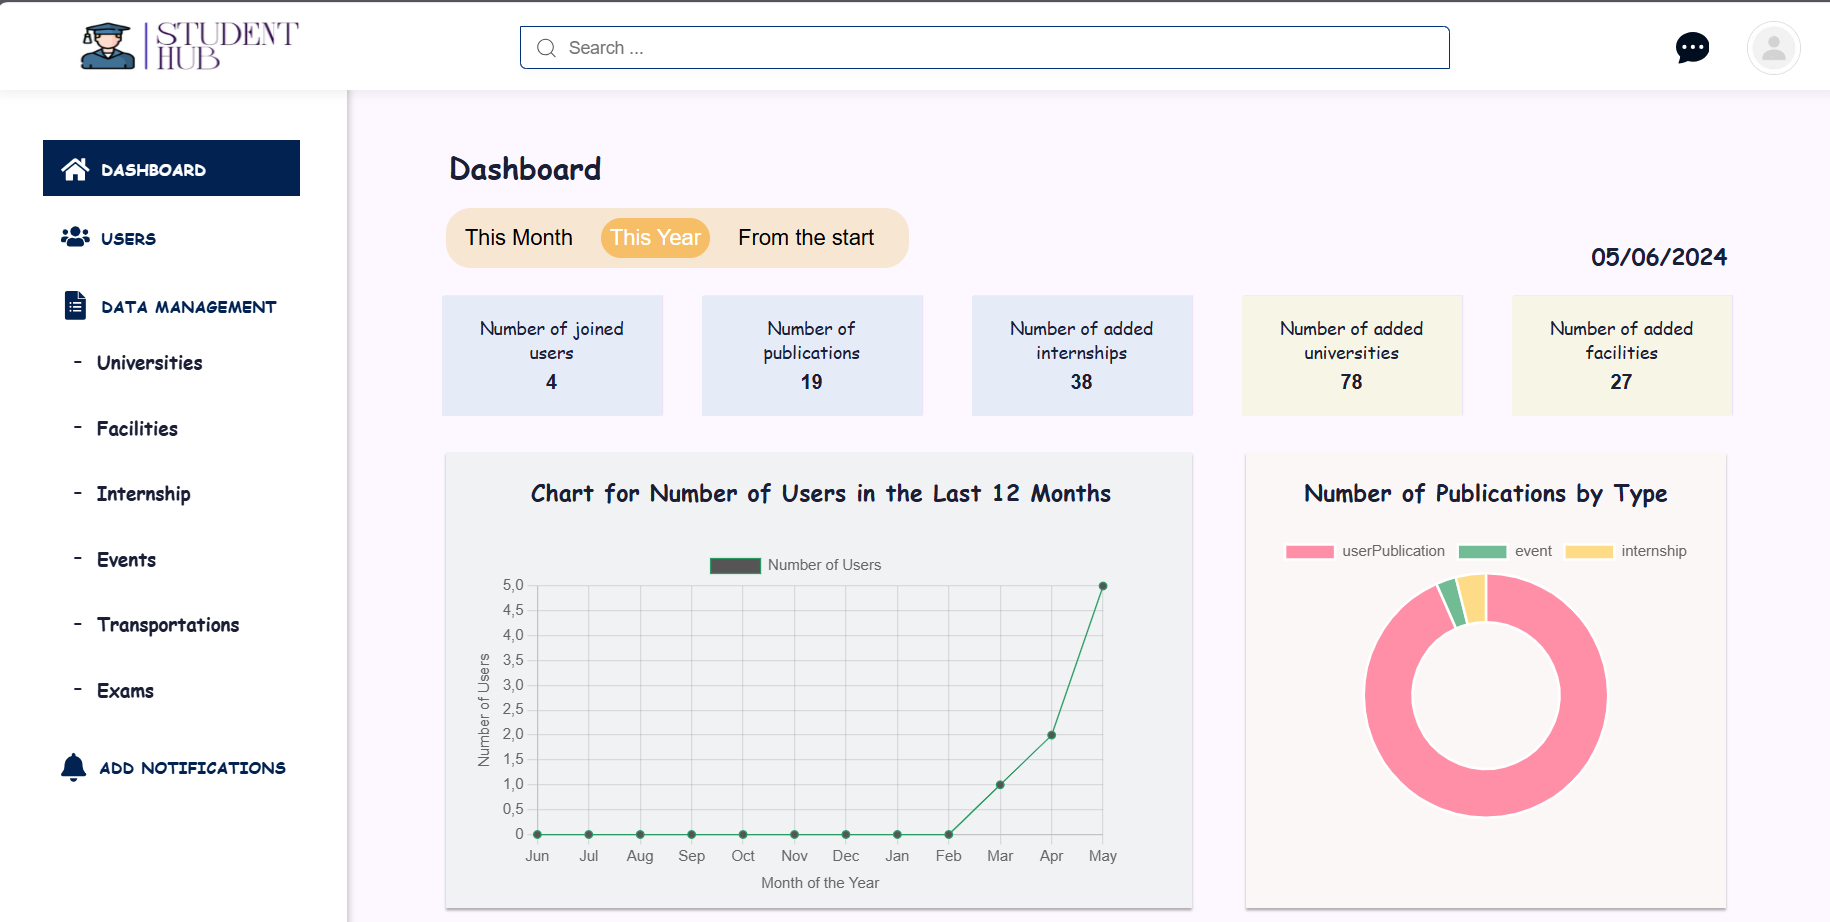
\includegraphics[height=8cm,width=15.5cm]{images/AAADashboard.png}%
    }
    \caption{Interace tableau de bord  }
\end{figure}

\section{La carte map }
\vspace{-4mm}
La carte interactive dans notre application mobile affiche la localisation des différentes Endroits disponibles pour les utilisateurs. En utilisant des marqueurs sur la carte, les utilisateurs peuvent visualiser facilement les emplacements des universités, des stations de transport, des lieux d'événements, et d'autres installations pertinentes. Cette fonctionnalité offre une expérience conviviale aux utilisateurs, leur permettant de naviguer efficacement dans leur environnement et de trouver les services qui les intéressent.

\begin{figure}[H]%
    \center%
    \setlength{\fboxsep}{5pt}%
    \setlength{\fboxrule}{0.5pt}%
    \fbox{
    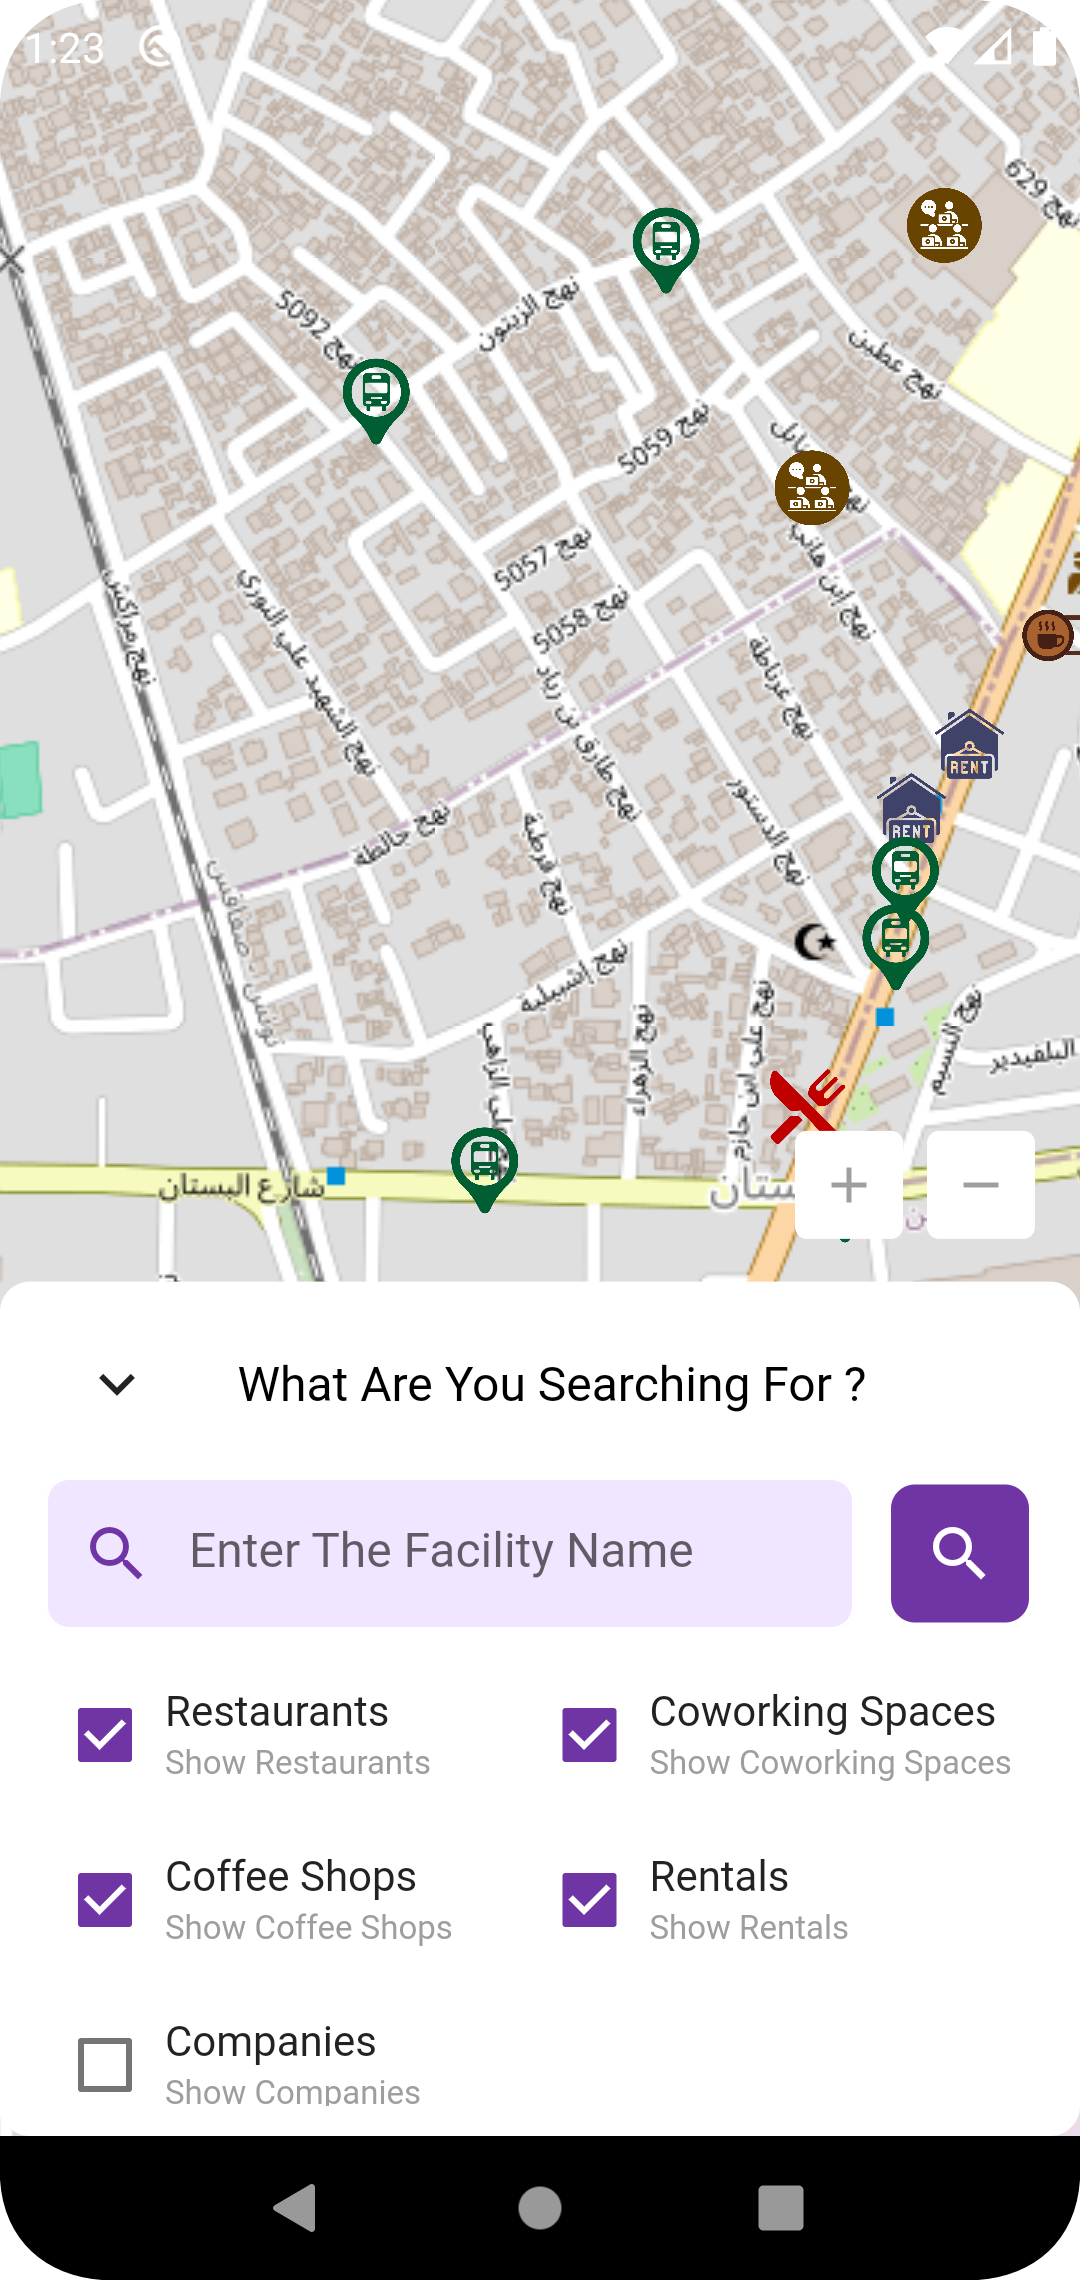
\includegraphics[height=10cm,width=7cm]{images/AAAMap.png}%
    }
    \caption{Interface carte map }
\end{figure}
\vspace{-1.2cm}
\section{Conclusion }
\vspace{-4mm}
En conclusion, ce sprint a été dédié à l'amélioration de la gestion des publications et des notifications au sein de notre application. En fournissant aux administrateurs des outils performants et intuitifs, notre objectif est de rehausser l'expérience utilisateur en optimisant la visibilité et la gestion des publications, ainsi qu'en rendant les notifications plus pertinentes et réactives. Ce sprint marque une étape importante dans notre engagement à offrir une plateforme dynamique et engageante pour nos utilisateurs

\end{sloppypar} 
 % Chapitre 11
    \chapter*{Conclusion générale et perspectives}
\markboth{\MakeUppercase{CONCLUSION GÉNÉRALE}}{}
\addcontentsline{toc}{chapter}{CONCLUSION GÉNÉRALE}
\adjustmtc
\begin{sloppypar} 
\thispagestyle{MyStyle}
Ce rapport résulte de notre immersion dans le projet de développement d'une application mobile permettant aux étudiants de créer un compte, de publier du contenu et de gérer leur profil. L'administrateur contrôle les données à partir d'une interface web dédiée.

Dès le début, notre objectif était de créer un système fluide et efficace. Nous avons développé une plateforme permettant aux utilisateurs de créer des comptes, de publier du contenu et de gérer leur profil, tandis que l'administrateur gère les données via une interface web dédiée.

En utilisant les technologies appropriées, nous avons pu développer une application mobile , offrant une expérience utilisateur optimale. L'application permet aux étudiants de publier du contenu et de gérer leur profil facilement, tandis que l'administrateur peut contrôler les données de manière efficace à partir de son interface web.

Nous sommes convaincus que cette expérience nous a permis d'acquérir des compétences précieuses en matière de développement d'applications mobiles et de gestion de bases de données. Ces compétences seront extrêmement bénéfiques pour notre avenir professionnel, nous permettant de relever de nouveaux défis avec confiance et compétence.. Envisageant l'avenir, l'intégration d'un chatbot pour répondre aux questions fréquentes des utilisateurs serait une étape logique pour améliorer davantage l'expérience utilisateur et enrichir notre plateforme.


\end{sloppypar}





























    \chapter*{Bibliographie}
\markboth{\MakeUppercase{Bibliographie}}{}
\addcontentsline{toc}{chapter}{Bibliographie}
\adjustmtc
\begin{sloppypar} 
\thispagestyle{MyStyle}


\begin{itemize}
    \item \textbf{Nom du livre} : SCRUM : le guide pratique de la méthode agile la plus populaire
    \begin{itemize}
        \item [•] \textbf{Maison d’édition} : DUNOD
        \item [•] \textbf{Auteur} : Claude Aubry
        \item [•] \textbf{ISBN} : 2100738747
        \item [•] \textbf{Date d‘édition} : 1\textsuperscript{er} octobre 2015
    \end{itemize}
    
    \item \textbf{Nom du livre} : UML 2 Analyse et Conception
    \begin{itemize}
        \item [•] \textbf{Maison d’édition} : DUNOD
        \item [•] \textbf{Auteur} : Joseph Gabay
        \item [•] \textbf{ISBN} : 9782100535675
        \item [•] \textbf{Date d‘édition} : 5\textsuperscript{ème} décembre 2005
    \end{itemize}

    \item \textbf{Nom du livre} : Android Programming: The Big Nerd Ranch Guide
    \begin{itemize}
        \item [•] \textbf{Maison d’édition} : Big Nerd Ranch
        \item [•] \textbf{Auteur} : Bill Phillips, Chris Stewart, Kristin Marsicano
        \item [•] \textbf{ISBN} : 9780134706054
        \item [•] \textbf{Date d‘édition} : 2017
    \end{itemize}

    \item \textbf{Nom du livre} : React Native in Action
    \begin{itemize}
        \item [•] \textbf{Maison d’édition} : Manning Publications
        \item [•] \textbf{Auteur} : Nader Dabit
        \item [•] \textbf{ISBN} : 9781617294051
        \item [•] \textbf{Date d‘édition} : 2019
    \end{itemize}

    \item \textbf{Nom du livre} : Database System Concepts
    \begin{itemize}
        \item [•] \textbf{Maison d’édition} : McGraw-Hill
        \item [•] \textbf{Auteur} : Abraham Silberschatz, Henry F. Korth, S. Sudarshan
        \item [•] \textbf{ISBN} : 9780073523323
        \item [•] \textbf{Date d‘édition} : 2010
    \end{itemize}

    \item \textbf{Nom du livre} : Spring Boot in Action
    \begin{itemize}
        \item [•] \textbf{Maison d’édition} : Manning Publications
        \item [•] \textbf{Auteur} : Craig Walls
        \item [•] \textbf{ISBN} : 9781617292545
        \item [•] \textbf{Date d‘édition} : 2016
    \end{itemize}
\end{itemize}
\end{sloppypar}
    \chapter*{Netographie}
\markboth{\MakeUppercase{Netographie}}{}
\addcontentsline{toc}{chapter}{Netographie}
\adjustmtc
\begin{sloppypar} 
\thispagestyle{MyStyle}
\small % Réduit la taille de la police


\begin{enumerate}
\item [1] \url{https://sabricole.developpez.com/uml/tutoriel/unifiedProcess/} consulté le 30/03/2024
\item [2] \url{https://www.planzone.fr/blog/quest-ce-que-la-methodologie-scrum} consulté le 12/03/2024
\item [3] \url{https://expertises.acadys.com/wp-content/uploads/2018/01/BP-N68-Scrum.pdf} consulté le 26/03/2024
\item [4] \url{https://www.lucidchart.com/} consulté le 24/03/2024
\item [5] \url{https://www.1min30.com/developpement-web-mobile/figma-1287540804} consulté le 13/03/2024
\item [6] \url{https://bility.fr/definition-visual-studio-code/} consulté le 03/04/2024
\item [7] \url{https://www.jetbrains.com/idea/features/} consulté le 13/03/2024
\item [8] \url{https://developer.android.com/studio/intro?hl=fr} consulté le 11/03/2024
\item [9] \url{https://bility.fr/definition-postman/} consulté le 22/03/2024
\item [10] \url{https://www.axopen.com/blog/2017/02/gitlab-cest-quoi/} consulté le 12/03/2024
\item [11] \url{https://www.50a.fr/0/react} consulté le 19/03/2024
\item [12] \url{https://www.merriam-webster.com/dictionary/flutter} consulté le 16/03/2024
\item [13] \url{https://developer.mozilla.org/fr/docs/Learn/JavaScript/First_steps/What_is_JavaScript} consulté le 02/04/2024
\item [14] \url{https://www.linternaute.fr/dictionnaire/fr/definition/dart/} consulté le 14/03/2024
\item [15] \url{https://www.ibm.com/fr-fr/topics/java-spring-boot} consulté le 24/03/2024
\item [16] \url{https://www.futura-sciences.com/tech/definitions/informatique-java-485//} consulté le 25/03/2024
\item [17] \url{https://www.lucidchart.com/pages/fr/diagramme-de-cas-dutilisation-uml} consulté le 15/03/2024
\item [18] \url{https://reactnative.dev/docs/getting-started} consulté le 10/05/2024
\item [19] \url{https://firebase.google.com/docs} consulté le 10/05/2024
\item [20] \url{https://docs.docker.com/} consulté le 10/05/2024
\item [21] \url{https://jestjs.io/docs/getting-started} consulté le 10/05/2024
\end{enumerate}
\end{sloppypar}


\end{document}
